%********************************************%
%*       Generated from PreTeXt source      *%
%*       on 2022-07-26T12:04:27-04:00       *%
%*   A recent stable commit (2020-08-09):   *%
%* 98f21740783f166a773df4dc83cab5293ab63a4a *%
%*                                          *%
%*         https://pretextbook.org          *%
%*                                          *%
%********************************************%
%% We elect to always write snapshot output into <job>.dep file
\RequirePackage{snapshot}
\documentclass[oneside,10pt,]{book}
%% Custom Preamble Entries, early (use latex.preamble.early)
%% Default LaTeX packages
%%   1.  always employed (or nearly so) for some purpose, or
%%   2.  a stylewriter may assume their presence
\usepackage{geometry}
%% Some aspects of the preamble are conditional,
%% the LaTeX engine is one such determinant
\usepackage{ifthen}
%% etoolbox has a variety of modern conveniences
\usepackage{etoolbox}
\usepackage{ifxetex,ifluatex}
%% Raster graphics inclusion
\usepackage{graphicx}
%% Color support, xcolor package
%% Always loaded, for: add/delete text, author tools
%% Here, since tcolorbox loads tikz, and tikz loads xcolor
\PassOptionsToPackage{usenames,dvipsnames,svgnames,table}{xcolor}
\usepackage{xcolor}
%% begin: defined colors, via xcolor package, for styling
%% end: defined colors, via xcolor package, for styling
%% Colored boxes, and much more, though mostly styling
%% skins library provides "enhanced" skin, employing tikzpicture
%% boxes may be configured as "breakable" or "unbreakable"
%% "raster" controls grids of boxes, aka side-by-side
\usepackage{tcolorbox}
\tcbuselibrary{skins}
\tcbuselibrary{breakable}
\tcbuselibrary{raster}
%% We load some "stock" tcolorbox styles that we use a lot
%% Placement here is provisional, there will be some color work also
%% First, black on white, no border, transparent, but no assumption about titles
\tcbset{ bwminimalstyle/.style={size=minimal, boxrule=-0.3pt, frame empty,
colback=white, colbacktitle=white, coltitle=black, opacityfill=0.0} }
%% Second, bold title, run-in to text/paragraph/heading
%% Space afterwards will be controlled by environment,
%% independent of constructions of the tcb title
%% Places \blocktitlefont onto many block titles
\tcbset{ runintitlestyle/.style={fonttitle=\blocktitlefont\upshape\bfseries, attach title to upper} }
%% Spacing prior to each exercise, anywhere
\tcbset{ exercisespacingstyle/.style={before skip={1.5ex plus 0.5ex}} }
%% Spacing prior to each block
\tcbset{ blockspacingstyle/.style={before skip={2.0ex plus 0.5ex}} }
%% xparse allows the construction of more robust commands,
%% this is a necessity for isolating styling and behavior
%% The tcolorbox library of the same name loads the base library
\tcbuselibrary{xparse}
%% The tcolorbox library loads TikZ, its calc package is generally useful,
%% and is necessary for some smaller documents that use partial tcolor boxes
%% See:  https://github.com/PreTeXtBook/pretext/issues/1624
\usetikzlibrary{calc}
%% Hyperref should be here, but likes to be loaded late
%%
%% Inline math delimiters, \(, \), need to be robust
%% 2016-01-31:  latexrelease.sty  supersedes  fixltx2e.sty
%% If  latexrelease.sty  exists, bugfix is in kernel
%% If not, bugfix is in  fixltx2e.sty
%% See:  https://tug.org/TUGboat/tb36-3/tb114ltnews22.pdf
%% and read "Fewer fragile commands" in distribution's  latexchanges.pdf
\IfFileExists{latexrelease.sty}{}{\usepackage{fixltx2e}}
%% Footnote counters and part/chapter counters are manipulated
%% April 2018:  chngcntr  commands now integrated into the kernel,
%% but circa 2018/2019 the package would still try to redefine them,
%% so we need to do the work of loading conditionally for old kernels.
%% From version 1.1a,  chngcntr  should detect defintions made by LaTeX kernel.
\ifdefined\counterwithin
\else
    \usepackage{chngcntr}
\fi
%% Text height identically 9 inches, text width varies on point size
%% See Bringhurst 2.1.1 on measure for recommendations
%% 75 characters per line (count spaces, punctuation) is target
%% which is the upper limit of Bringhurst's recommendations
\geometry{letterpaper,total={340pt,9.0in}}
%% Custom Page Layout Adjustments (use latex.geometry)
%% This LaTeX file may be compiled with pdflatex, xelatex, or lualatex executables
%% LuaTeX is not explicitly supported, but we do accept additions from knowledgeable users
%% The conditional below provides  pdflatex  specific configuration last
%% begin: engine-specific capabilities
\ifthenelse{\boolean{xetex} \or \boolean{luatex}}{%
%% begin: xelatex and lualatex-specific default configuration
\ifxetex\usepackage{xltxtra}\fi
%% realscripts is the only part of xltxtra relevant to lualatex 
\ifluatex\usepackage{realscripts}\fi
%% end:   xelatex and lualatex-specific default configuration
}{
%% begin: pdflatex-specific default configuration
%% We assume a PreTeXt XML source file may have Unicode characters
%% and so we ask LaTeX to parse a UTF-8 encoded file
%% This may work well for accented characters in Western language,
%% but not with Greek, Asian languages, etc.
%% When this is not good enough, switch to the  xelatex  engine
%% where Unicode is better supported (encouraged, even)
\usepackage[utf8]{inputenc}
%% end: pdflatex-specific default configuration
}
%% end:   engine-specific capabilities
%%
%% Fonts.  Conditional on LaTex engine employed.
%% Default Text Font: The Latin Modern fonts are
%% "enhanced versions of the [original TeX] Computer Modern fonts."
%% We use them as the default text font for PreTeXt output.
%% Default Monospace font: Inconsolata (aka zi4)
%% Sponsored by TUG: http://levien.com/type/myfonts/inconsolata.html
%% Loaded for documents with intentional objects requiring monospace
%% See package documentation for excellent instructions
%% fontspec will work universally if we use filename to locate OTF files
%% Loads the "upquote" package as needed, so we don't have to
%% Upright quotes might come from the  textcomp  package, which we also use
%% We employ the shapely \ell to match Google Font version
%% pdflatex: "varl" package option produces shapely \ell
%% pdflatex: "var0" package option produces plain zero (not used)
%% pdflatex: "varqu" package option produces best upright quotes
%% xelatex,lualatex: add OTF StylisticSet 1 for shapely \ell
%% xelatex,lualatex: add OTF StylisticSet 2 for plain zero (not used)
%% xelatex,lualatex: add OTF StylisticSet 3 for upright quotes
%%
%% Automatic Font Control
%% Portions of a document, are, or may, be affected by defined commands
%% These are perhaps more flexible when using  xelatex  rather than  pdflatex
%% The following definitions are meant to be re-defined in a style, using \renewcommand
%% They are scoped when employed (in a TeX group), and so should not be defined with an argument
\newcommand{\divisionfont}{\relax}
\newcommand{\blocktitlefont}{\relax}
\newcommand{\contentsfont}{\relax}
\newcommand{\pagefont}{\relax}
\newcommand{\tabularfont}{\relax}
\newcommand{\xreffont}{\relax}
\newcommand{\titlepagefont}{\relax}
%%
\ifthenelse{\boolean{xetex} \or \boolean{luatex}}{%
%% begin: font setup and configuration for use with xelatex
%% Generally, xelatex is necessary for non-Western fonts
%% fontspec package provides extensive control of system fonts,
%% meaning *.otf (OpenType), and apparently *.ttf (TrueType)
%% that live *outside* your TeX/MF tree, and are controlled by your *system*
%% (it is possible that a TeX distribution will place fonts in a system location)
%%
%% The fontspec package is the best vehicle for using different fonts in  xelatex
%% So we load it always, no matter what a publisher or style might want
%%
\usepackage{fontspec}
%%
%% begin: xelatex main font ("font-xelatex-main" template)
%% Latin Modern Roman is the default font for xelatex and so is loaded with a TU encoding
%% *in the format* so we can't touch it, only perhaps adjust it later
%% in one of two ways (then known by NFSS names such as "lmr")
%% (1) via NFSS with font family names such as "lmr" and "lmss"
%% (2) via fontspec with commands like \setmainfont{Latin Modern Roman}
%% The latter requires the font to be known at the system-level by its font name,
%% but will give access to OTF font features through optional arguments
%% https://tex.stackexchange.com/questions/470008/
%% where-and-how-does-fontspec-sty-specify-the-default-font-latin-modern-roman
%% http://tex.stackexchange.com/questions/115321
%% /how-to-optimize-latin-modern-font-with-xelatex
%%
%% end:   xelatex main font ("font-xelatex-main" template)
%% begin: xelatex mono font ("font-xelatex-mono" template)
%% (conditional on non-trivial uses being present in source)
\IfFontExistsTF{Inconsolatazi4-Regular.otf}{}{\GenericError{}{The font "Inconsolatazi4-Regular.otf" requested by PreTeXt output is not available.  Either a file cannot be located in default locations via a filename, or a font is not known by its name as part of your system.}{Consult the PreTeXt Guide for help with LaTeX fonts.}{}}
\IfFontExistsTF{Inconsolatazi4-Bold.otf}{}{\GenericError{}{The font "Inconsolatazi4-Bold.otf" requested by PreTeXt output is not available.  Either a file cannot be located in default locations via a filename, or a font is not known by its name as part of your system.}{Consult the PreTeXt Guide for help with LaTeX fonts.}{}}
\usepackage{zi4}
\setmonofont[BoldFont=Inconsolatazi4-Bold.otf,StylisticSet={1,3}]{Inconsolatazi4-Regular.otf}
%% end:   xelatex mono font ("font-xelatex-mono" template)
%% begin: xelatex font adjustments ("font-xelatex-style" template)
%% end:   xelatex font adjustments ("font-xelatex-style" template)
%%
%% Extensive support for other languages
\usepackage{polyglossia}
%% Set main/default language based on pretext/@xml:lang value
%% document language code is "en-US", US English
%% usmax variant has extra hypenation
\setmainlanguage[variant=usmax]{english}
%% Enable secondary languages based on discovery of @xml:lang values
%% Enable fonts/scripts based on discovery of @xml:lang values
%% Western languages should be ably covered by Latin Modern Roman
%% end:   font setup and configuration for use with xelatex
}{%
%% begin: font setup and configuration for use with pdflatex
%% begin: pdflatex main font ("font-pdflatex-main" template)
\usepackage{lmodern}
\usepackage[T1]{fontenc}
%% end:   pdflatex main font ("font-pdflatex-main" template)
%% begin: pdflatex mono font ("font-pdflatex-mono" template)
%% (conditional on non-trivial uses being present in source)
\usepackage[varqu,varl]{inconsolata}
%% end:   pdflatex mono font ("font-pdflatex-mono" template)
%% begin: pdflatex font adjustments ("font-pdflatex-style" template)
%% end:   pdflatex font adjustments ("font-pdflatex-style" template)
%% end:   font setup and configuration for use with pdflatex
}
%% Micromanage spacing, etc.  The named "microtype-options"
%% template may be employed to fine-tune package behavior
\usepackage{microtype}
%% Symbols, align environment, commutative diagrams, bracket-matrix
\usepackage{amsmath}
\usepackage{amscd}
\usepackage{amssymb}
%% allow page breaks within display mathematics anywhere
%% level 4 is maximally permissive
%% this is exactly the opposite of AMSmath package philosophy
%% there are per-display, and per-equation options to control this
%% split, aligned, gathered, and alignedat are not affected
\allowdisplaybreaks[4]
%% allow more columns to a matrix
%% can make this even bigger by overriding with  latex.preamble.late  processing option
\setcounter{MaxMatrixCols}{30}
%%
%%
%% Division Titles, and Page Headers/Footers
%% titlesec package, loading "titleps" package cooperatively
%% See code comments about the necessity and purpose of "explicit" option.
%% The "newparttoc" option causes a consistent entry for parts in the ToC 
%% file, but it is only effective if there is a \titleformat for \part.
%% "pagestyles" loads the  titleps  package cooperatively.
\usepackage[explicit, newparttoc, pagestyles]{titlesec}
%% The companion titletoc package for the ToC.
\usepackage{titletoc}
%% Fixes a bug with transition from chapters to appendices in a "book"
%% See generating XSL code for more details about necessity
\newtitlemark{\chaptertitlename}
%% begin: customizations of page styles via the modal "titleps-style" template
%% Designed to use commands from the LaTeX "titleps" package
%% Plain pages should have the same font for page numbers
\renewpagestyle{plain}{%
\setfoot{}{\pagefont\thepage}{}%
}%
%% Single pages as in default LaTeX
\renewpagestyle{headings}{%
\sethead{\pagefont\slshape\MakeUppercase{\ifthechapter{\chaptertitlename\space\thechapter.\space}{}\chaptertitle}}{}{\pagefont\thepage}%
}%
\pagestyle{headings}
%% end: customizations of page styles via the modal "titleps-style" template
%%
%% Create globally-available macros to be provided for style writers
%% These are redefined for each occurence of each division
\newcommand{\divisionnameptx}{\relax}%
\newcommand{\titleptx}{\relax}%
\newcommand{\subtitleptx}{\relax}%
\newcommand{\shortitleptx}{\relax}%
\newcommand{\authorsptx}{\relax}%
\newcommand{\epigraphptx}{\relax}%
%% Create environments for possible occurences of each division
%% Environment for a PTX "preface" at the level of a LaTeX "chapter"
\NewDocumentEnvironment{preface}{mmmmmm}
{%
\renewcommand{\divisionnameptx}{Preface}%
\renewcommand{\titleptx}{#1}%
\renewcommand{\subtitleptx}{#2}%
\renewcommand{\shortitleptx}{#3}%
\renewcommand{\authorsptx}{#4}%
\renewcommand{\epigraphptx}{#5}%
\chapter*{#1}%
\addcontentsline{toc}{chapter}{#3}
\label{#6}%
}{}%
%% Environment for a PTX "section" at the level of a LaTeX "section"
\NewDocumentEnvironment{sectionptx}{mmmmmm}
{%
\renewcommand{\divisionnameptx}{Section}%
\renewcommand{\titleptx}{#1}%
\renewcommand{\subtitleptx}{#2}%
\renewcommand{\shortitleptx}{#3}%
\renewcommand{\authorsptx}{#4}%
\renewcommand{\epigraphptx}{#5}%
\section[{#3}]{#1}%
\label{#6}%
}{}%
%% Environment for a PTX "subsection" at the level of a LaTeX "subsection"
\NewDocumentEnvironment{subsectionptx}{mmmmmm}
{%
\renewcommand{\divisionnameptx}{Subsection}%
\renewcommand{\titleptx}{#1}%
\renewcommand{\subtitleptx}{#2}%
\renewcommand{\shortitleptx}{#3}%
\renewcommand{\authorsptx}{#4}%
\renewcommand{\epigraphptx}{#5}%
\subsection[{#3}]{#1}%
\label{#6}%
}{}%
%% Environment for a PTX "chapter" at the level of a LaTeX "chapter"
\NewDocumentEnvironment{chapterptx}{mmmmmm}
{%
\renewcommand{\divisionnameptx}{Chapter}%
\renewcommand{\titleptx}{#1}%
\renewcommand{\subtitleptx}{#2}%
\renewcommand{\shortitleptx}{#3}%
\renewcommand{\authorsptx}{#4}%
\renewcommand{\epigraphptx}{#5}%
\chapter[{#3}]{#1}%
\label{#6}%
}{}%
%% Environment for a PTX "subsubsection" at the level of a LaTeX "subsubsection"
\NewDocumentEnvironment{subsubsectionptx}{mmmmmm}
{%
\renewcommand{\divisionnameptx}{Subsubsection}%
\renewcommand{\titleptx}{#1}%
\renewcommand{\subtitleptx}{#2}%
\renewcommand{\shortitleptx}{#3}%
\renewcommand{\authorsptx}{#4}%
\renewcommand{\epigraphptx}{#5}%
\subsubsection[{#3}]{#1}%
\label{#6}%
}{}%
%%
%% Styles for six traditional LaTeX divisions
\titleformat{\part}[display]
{\divisionfont\Huge\bfseries\centering}{\divisionnameptx\space\thepart}{30pt}{\Huge#1}
[{\Large\centering\authorsptx}]
\titleformat{\chapter}[display]
{\divisionfont\huge\bfseries}{\divisionnameptx\space\thechapter}{20pt}{\Huge#1}
[{\Large\authorsptx}]
\titleformat{name=\chapter,numberless}[display]
{\divisionfont\huge\bfseries}{}{0pt}{#1}
[{\Large\authorsptx}]
\titlespacing*{\chapter}{0pt}{50pt}{40pt}
\titleformat{\section}[hang]
{\divisionfont\Large\bfseries}{\thesection}{1ex}{#1}
[{\large\authorsptx}]
\titleformat{name=\section,numberless}[block]
{\divisionfont\Large\bfseries}{}{0pt}{#1}
[{\large\authorsptx}]
\titlespacing*{\section}{0pt}{3.5ex plus 1ex minus .2ex}{2.3ex plus .2ex}
\titleformat{\subsection}[hang]
{\divisionfont\large\bfseries}{\thesubsection}{1ex}{#1}
[{\normalsize\authorsptx}]
\titleformat{name=\subsection,numberless}[block]
{\divisionfont\large\bfseries}{}{0pt}{#1}
[{\normalsize\authorsptx}]
\titlespacing*{\subsection}{0pt}{3.25ex plus 1ex minus .2ex}{1.5ex plus .2ex}
\titleformat{\subsubsection}[hang]
{\divisionfont\normalsize\bfseries}{\thesubsubsection}{1em}{#1}
[{\small\authorsptx}]
\titleformat{name=\subsubsection,numberless}[block]
{\divisionfont\normalsize\bfseries}{}{0pt}{#1}
[{\normalsize\authorsptx}]
\titlespacing*{\subsubsection}{0pt}{3.25ex plus 1ex minus .2ex}{1.5ex plus .2ex}
\titleformat{\paragraph}[hang]
{\divisionfont\normalsize\bfseries}{\theparagraph}{1em}{#1}
[{\small\authorsptx}]
\titleformat{name=\paragraph,numberless}[block]
{\divisionfont\normalsize\bfseries}{}{0pt}{#1}
[{\normalsize\authorsptx}]
\titlespacing*{\paragraph}{0pt}{3.25ex plus 1ex minus .2ex}{1.5em}
%%
%% Styles for five traditional LaTeX divisions
\titlecontents{part}%
[0pt]{\contentsmargin{0em}\addvspace{1pc}\contentsfont\bfseries}%
{\Large\thecontentslabel\enspace}{\Large}%
{}%
[\addvspace{.5pc}]%
\titlecontents{chapter}%
[0pt]{\contentsmargin{0em}\addvspace{1pc}\contentsfont\bfseries}%
{\large\thecontentslabel\enspace}{\large}%
{\hfill\bfseries\thecontentspage}%
[\addvspace{.5pc}]%
\dottedcontents{section}[3.8em]{\contentsfont}{2.3em}{1pc}%
\dottedcontents{subsection}[6.1em]{\contentsfont}{3.2em}{1pc}%
\dottedcontents{subsubsection}[9.3em]{\contentsfont}{4.3em}{1pc}%
%%
%% Begin: Semantic Macros
%% To preserve meaning in a LaTeX file
%%
%% \mono macro for content of "c", "cd", "tag", etc elements
%% Also used automatically in other constructions
%% Simply an alias for \texttt
%% Always defined, even if there is no need, or if a specific tt font is not loaded
\newcommand{\mono}[1]{\texttt{#1}}
%%
%% Following semantic macros are only defined here if their
%% use is required only in this specific document
%%
%% Used for inline definitions of terms
\newcommand{\terminology}[1]{\textbf{#1}}
%% End: Semantic Macros
%% Localize LaTeX supplied names (possibly none)
\renewcommand*{\chaptername}{Chapter}
%% Equation Numbering
%% Controlled by  numbering.equations.level  processing parameter
%% No adjustment here implies document-wide numbering
\numberwithin{equation}{section}
%% "tcolorbox" environment for a single image, occupying entire \linewidth
%% arguments are left-margin, width, right-margin, as multiples of
%% \linewidth, and are guaranteed to be positive and sum to 1.0
\tcbset{ imagestyle/.style={bwminimalstyle} }
\NewTColorBox{image}{mmm}{imagestyle,left skip=#1\linewidth,width=#2\linewidth}
%% For improved tables
\usepackage{array}
%% Some extra height on each row is desirable, especially with horizontal rules
%% Increment determined experimentally
\setlength{\extrarowheight}{0.2ex}
%% Define variable thickness horizontal rules, full and partial
%% Thicknesses are 0.03, 0.05, 0.08 in the  booktabs  package
\newcommand{\hrulethin}  {\noalign{\hrule height 0.04em}}
\newcommand{\hrulemedium}{\noalign{\hrule height 0.07em}}
\newcommand{\hrulethick} {\noalign{\hrule height 0.11em}}
%% We preserve a copy of the \setlength package before other
%% packages (extpfeil) get a chance to load packages that redefine it
\let\oldsetlength\setlength
\newlength{\Oldarrayrulewidth}
\newcommand{\crulethin}[1]%
{\noalign{\global\oldsetlength{\Oldarrayrulewidth}{\arrayrulewidth}}%
\noalign{\global\oldsetlength{\arrayrulewidth}{0.04em}}\cline{#1}%
\noalign{\global\oldsetlength{\arrayrulewidth}{\Oldarrayrulewidth}}}%
\newcommand{\crulemedium}[1]%
{\noalign{\global\oldsetlength{\Oldarrayrulewidth}{\arrayrulewidth}}%
\noalign{\global\oldsetlength{\arrayrulewidth}{0.07em}}\cline{#1}%
\noalign{\global\oldsetlength{\arrayrulewidth}{\Oldarrayrulewidth}}}
\newcommand{\crulethick}[1]%
{\noalign{\global\oldsetlength{\Oldarrayrulewidth}{\arrayrulewidth}}%
\noalign{\global\oldsetlength{\arrayrulewidth}{0.11em}}\cline{#1}%
\noalign{\global\oldsetlength{\arrayrulewidth}{\Oldarrayrulewidth}}}
%% Single letter column specifiers defined via array package
\newcolumntype{A}{!{\vrule width 0.04em}}
\newcolumntype{B}{!{\vrule width 0.07em}}
\newcolumntype{C}{!{\vrule width 0.11em}}
%% tcolorbox to place tabular outside of a sidebyside
\tcbset{ tabularboxstyle/.style={bwminimalstyle,} }
\newtcolorbox{tabularbox}[3]{tabularboxstyle, left skip=#1\linewidth, width=#2\linewidth,}
%% Footnote Numbering
%% Specified by numbering.footnotes.level
%% Undo counter reset by chapter for a book
\counterwithout{footnote}{chapter}
\counterwithin*{footnote}{section}
%% More flexible list management, esp. for references
%% But also for specifying labels (i.e. custom order) on nested lists
\usepackage{enumitem}
%% hyperref driver does not need to be specified, it will be detected
%% Footnote marks in tcolorbox have broken linking under
%% hyperref, so it is necessary to turn off all linking
%% It *must* be given as a package option, not with \hypersetup
\usepackage[hyperfootnotes=false]{hyperref}
%% configure hyperref's  \href{}{}  and  \nolinkurl  to match listings' inline verbatim
\renewcommand\UrlFont{\small\ttfamily}
%% Hyperlinking active in electronic PDFs, all links without surrounding boxes and blue
\hypersetup{colorlinks=true,linkcolor=blue,citecolor=blue,filecolor=blue,urlcolor=blue}
\hypersetup{pdftitle={OpenStax Calculus}}
%% If you manually remove hyperref, leave in this next command
%% This will allow LaTeX compilation, employing this no-op command
\providecommand\phantomsection{}
%% Division Numbering: Chapters, Sections, Subsections, etc
%% Division numbers may be turned off at some level ("depth")
%% A section *always* has depth 1, contrary to us counting from the document root
%% The latex default is 3.  If a larger number is present here, then
%% removing this command may make some cross-references ambiguous
%% The precursor variable $numbering-maxlevel is checked for consistency in the common XSL file
\setcounter{secnumdepth}{3}
%%
%% AMS "proof" environment is no longer used, but we leave previously
%% implemented \qedhere in place, should the LaTeX be recycled
\newcommand{\qedhere}{\relax}
%%
%% A faux tcolorbox whose only purpose is to provide common numbering
%% facilities for most blocks (possibly not projects, 2D displays)
%% Controlled by  numbering.theorems.level  processing parameter
\newtcolorbox[auto counter, number within=chapter]{block}{}
%%
%% This document is set to number PROJECT-LIKE on a separate numbering scheme
%% So, a faux tcolorbox whose only purpose is to provide this numbering
%% Controlled by  numbering.projects.level  processing parameter
\newtcolorbox[auto counter, number within=section]{project-distinct}{}
%% A faux tcolorbox whose only purpose is to provide common numbering
%% facilities for 2D displays which are subnumbered as part of a "sidebyside"
\makeatletter
\newtcolorbox[auto counter, number within=tcb@cnt@block, number freestyle={\noexpand\thetcb@cnt@block(\noexpand\alph{\tcbcounter})}]{subdisplay}{}
\makeatother
%%
%% tcolorbox, with styles, for THEOREM-LIKE
%%
%% theorem: fairly simple numbered block/structure
\tcbset{ theoremstyle/.style={bwminimalstyle, runintitlestyle, blockspacingstyle, after title={\space}, } }
\newtcolorbox[use counter from=block]{theorem}[3]{title={{Theorem~\thetcbcounter\notblank{#1#2}{\space}{}\notblank{#1}{\space#1}{}\notblank{#2}{\space(#2)}{}}}, phantomlabel={#3}, breakable, parbox=false, after={\par}, fontupper=\itshape, theoremstyle, }
%%
%% tcolorbox, with styles, for PROOF-LIKE
%%
%% proof: title is a replacement
\tcbset{ proofstyle/.style={bwminimalstyle, fonttitle=\blocktitlefont\itshape, attach title to upper, after title={\space}, after upper={\space\space\hspace*{\stretch{1}}\(\blacksquare\)},
} }
\newtcolorbox{proof}[2]{title={\notblank{#1}{#1}{Proof.}}, phantom={\hypertarget{#2}{}}, breakable, parbox=false, after={\par}, proofstyle }
%%
%% tcolorbox, with styles, for DEFINITION-LIKE
%%
%% definition: fairly simple numbered block/structure
\tcbset{ definitionstyle/.style={bwminimalstyle, runintitlestyle, blockspacingstyle, after title={\space}, after upper={\space\space\hspace*{\stretch{1}}\(\lozenge\)}, } }
\newtcolorbox[use counter from=block]{definition}[2]{title={{Definition~\thetcbcounter\notblank{#1}{\space\space#1}{}}}, phantomlabel={#2}, breakable, parbox=false, after={\par}, definitionstyle, }
%%
%% tcolorbox, with styles, for REMARK-LIKE
%%
%% note: fairly simple numbered block/structure
\tcbset{ notestyle/.style={bwminimalstyle, runintitlestyle, blockspacingstyle, after title={\space}, } }
\newtcolorbox[use counter from=block]{note}[2]{title={{Note~\thetcbcounter\notblank{#1}{\space\space#1}{}}}, phantomlabel={#2}, breakable, parbox=false, after={\par}, notestyle, }
%%
%% tcolorbox, with styles, for EXAMPLE-LIKE
%%
%% example: fairly simple numbered block/structure
\tcbset{ examplestyle/.style={bwminimalstyle, runintitlestyle, blockspacingstyle, after title={\space}, after upper={\space\space\hspace*{\stretch{1}}\(\square\)}, } }
\newtcolorbox[use counter from=block]{example}[2]{title={{Example~\thetcbcounter\notblank{#1}{\space\space#1}{}}}, phantomlabel={#2}, breakable, parbox=false, after={\par}, examplestyle, }
%%
%% tcolorbox, with styles, for inline exercises
%%
%% inlineexercise: fairly simple numbered block/structure
\tcbset{ inlineexercisestyle/.style={bwminimalstyle, runintitlestyle, blockspacingstyle, after title={\space}, } }
\newtcolorbox[use counter from=block]{inlineexercise}[2]{title={{Checkpoint~\thetcbcounter\notblank{#1}{\space\space#1}{}}}, phantomlabel={#2}, breakable, parbox=false, after={\par}, inlineexercisestyle, }
%%
%% tcolorbox, with styles, for FIGURE-LIKE
%%
%% figureptx: 2-D display structure
\tcbset{ figureptxstyle/.style={bwminimalstyle, middle=1ex, blockspacingstyle, fontlower=\blocktitlefont} }
\newtcolorbox[use counter from=block]{figureptx}[3]{lower separated=false, before lower={{\textbf{Figure~\thetcbcounter}\space#1}}, phantomlabel={#2}, unbreakable, parbox=false, figureptxstyle, }
%% tableptx: 2-D display structure
\tcbset{ tableptxstyle/.style={bwminimalstyle, middle=1ex, blockspacingstyle, coltitle=black, bottomtitle=2ex, titlerule=-0.3pt, fonttitle=\blocktitlefont} }
\newtcolorbox[use counter from=block]{tableptx}[3]{title={{\textbf{Table~\thetcbcounter}\space#1}}, phantomlabel={#2}, unbreakable, parbox=false, tableptxstyle, }
%%
%% xparse environments for introductions and conclusions of divisions
%%
%% introduction: in a structured division
\NewDocumentEnvironment{introduction}{m}
{\notblank{#1}{\noindent\textbf{#1}\space}{}}{\par\medskip}
%%
%% tcolorbox, with styles, for miscellaneous environments
%%
%% back colophon, at the very end, typically on its own page
\tcbset{ backcolophonstyle/.style={bwminimalstyle, blockspacingstyle, before skip=5ex, left skip=0.15\textwidth, right skip=0.15\textwidth, fonttitle=\blocktitlefont\large\bfseries, center title, halign=center, bottomtitle=2ex} }
\newtcolorbox{backcolophon}[1]{title={Colophon}, phantom={\hypertarget{#1}{}}, breakable, parbox=false, backcolophonstyle}
%% Graphics Preamble Entries
\usepackage{tikz, pgfplots}
\usetikzlibrary{positioning,matrix,arrows}
\usetikzlibrary{shapes,decorations,shadows,fadings,patterns}
\usetikzlibrary{decorations.markings}
%% If tikz has been loaded, replace ampersand with \amp macro
%% extpfeil package for certain extensible arrows,
%% as also provided by MathJax extension of the same name
%% NB: this package loads mtools, which loads calc, which redefines
%%     \setlength, so it can be removed if it seems to be in the 
%%     way and your math does not use:
%%     
%%     \xtwoheadrightarrow, \xtwoheadleftarrow, \xmapsto, \xlongequal, \xtofrom
%%     
%%     we have had to be extra careful with variable thickness
%%     lines in tables, and so also load this package late
\usepackage{extpfeil}
%% Custom Preamble Entries, late (use latex.preamble.late)
%% Begin: Author-provided packages
%% (From  docinfo/latex-preamble/package  elements)
%% End: Author-provided packages
%% Begin: Author-provided macros
%% (From  docinfo/macros  element)
%% Plus three from PTX for XML characters
\newcommand{\N}{\mathbb N}
\newcommand{\Z}{\mathbb Z}
\newcommand{\Q}{\mathbb Q}
\newcommand{\R}{\mathbb R}
\newcommand{\lt}{<}
\newcommand{\gt}{>}
\newcommand{\amp}{&}
%% End: Author-provided macros
\begin{document}
%% bottom alignment is explicit, since it normally depends on oneside, twoside
\raggedbottom
\frontmatter
%% begin: half-title
\thispagestyle{empty}
{\titlepagefont\centering
\vspace*{0.28\textheight}
{\Huge OpenStax Calculus}\\[2\baselineskip]
{\LARGE Volume 1}\\
}
\clearpage
%% end:   half-title
%% begin: title page
%% Inspired by Peter Wilson's "titleDB" in "titlepages" CTAN package
\thispagestyle{empty}
{\titlepagefont\centering
\vspace*{0.14\textheight}
%% Target for xref to top-level element is ToC
\addtocontents{toc}{\protect\hypertarget{x:book:my-great-book}{}}
{\Huge OpenStax Calculus}\\[\baselineskip]
{\LARGE Volume 1}\\[3\baselineskip]
{\Large Custom Business Calculus Edition}\\[3\baselineskip]
{\Large July 26, 2022}\\}
\clearpage
%% end:   title page
%% begin: copyright-page
\thispagestyle{empty}
\hypertarget{g:colophon:idm1622950888}{}\vspace*{\stretch{2}}
\noindent{\bfseries Website}: \href{https:\slash{}\slash{}openstax.org\slash{}details\slash{}books\slash{}calculus-volume-1}{\mono{openstax.org/details/books/calculus-volume-1}}\par\medskip
\noindent\textcopyright{}2020\quad{}Rice University\\[0.5\baselineskip]
 Calculus Volumes 1, 2, and 3 are licensed under an Attribution-NonCommercial-Sharealike 4.0 International License (CC BY-NC-SA), which means you can share, remix, transform, and build upon the content, as long as you credit OpenStax and license your new creations under the same terms. To view a copy of this license, visit \href{http://creativecommons.org/licenses/by-sa/4.0/}{CreativeCommons.org}\footnote{\nolinkurl{creativecommons.org/licenses/by-sa/4.0}\label{g:fn:idm1622771432}}\par\medskip
\vspace*{\stretch{1}}
\null\clearpage
%% end:   copyright-page
%
%
\typeout{************************************************}
\typeout{Preface  Preface: OpenStax Calculus Volume 1}
\typeout{************************************************}
%
\begin{preface}{Preface: OpenStax Calculus Volume 1}{}{Preface: OpenStax Calculus Volume 1}{}{}{x:preface:meta_frontmatter-preface}
Welcome to \emph{Calculus Volume 1}, an OpenStax resource. This textbook was written to increase student access to high-quality learning materials, maintaining highest standards of academic rigor at little to no cost.%
%
%
\typeout{************************************************}
\typeout{Section 1 About OpenStax}
\typeout{************************************************}
%
\begin{sectionptx}{About OpenStax}{}{About OpenStax}{}{}{g:section:idm1622769128}
OpenStax is a nonprofit based at Rice University, and it’s our mission to improve student access to education. Our first openly licensed college textbook was published in 2012, and our library has since scaled to over 25 books for college and AP\textregistered{} courses used by hundreds of thousands of students. OpenStax Tutor, our low-cost personalized learning tool, is being used in college courses throughout the country.  Through our partnerships with philanthropic foundations and our alliance with other educational resource organizations, OpenStax is breaking down the most common barriers to learning and empowering students and instructors to succeed.%
\end{sectionptx}
%
%
\typeout{************************************************}
\typeout{Section 2 About OpenStax's resources}
\typeout{************************************************}
%
\begin{sectionptx}{About OpenStax's resources}{}{About OpenStax's resources}{}{}{g:section:idm1622765928}
%
%
\typeout{************************************************}
\typeout{Subsection 2.1 Customization}
\typeout{************************************************}
%
\begin{subsectionptx}{Customization}{}{Customization}{}{}{g:subsection:idm1622767976}
\emph{Calculus Volume 1} is licensed under a Creative Commons Attribution-NonCommercial-ShareAlike 4.0 International (CC-BY-NC-SA) license, which means that you can distribute, remix, and build upon the content, as long as you provide attribution to OpenStax and its content contributors, do not use the content for commercial purposes, and distribute the content under the same CC-BY-NC-SA license.%
\par
Because our books are openly licensed, you are free to use the entire book or pick and choose the sections that are most relevant to the needs of your course. Feel free to remix the content by assigning your students certain chapters and sections in your syllabus, in the order that you prefer. You can even provide a direct link in your syllabus to the sections in the web view of your book.%
\par
Instructors also have the option of creating a customized version of their OpenStax book. The custom version can be made available to students in low-cost print or digital form through their campus bookstore. Visit your book page on OpenStax.org for more information.%
\end{subsectionptx}
%
%
\typeout{************************************************}
\typeout{Subsection 2.2 Errata}
\typeout{************************************************}
%
\begin{subsectionptx}{Errata}{}{Errata}{}{}{g:subsection:idm1622761448}
All OpenStax textbooks undergo a rigorous review process. However, like any professional-grade textbook, errors sometimes occur. Since our books are web based, we can make updates periodically when deemed pedagogically necessary. If you have a correction to suggest, submit it through the link on your book page on OpenStax.org. Subject matter experts review all errata suggestions. OpenStax is committed to remaining transparent about all updates, so you will also find a list of past errata changes on your book page on OpenStax.org.%
\end{subsectionptx}
%
%
\typeout{************************************************}
\typeout{Subsection 2.3 Format}
\typeout{************************************************}
%
\begin{subsectionptx}{Format}{}{Format}{}{}{g:subsection:idm1622761960}
You can access this textbook for free in web view or PDF through OpenStax.org, and for a low cost in print.%
\end{subsectionptx}
\end{sectionptx}
%
%
\typeout{************************************************}
\typeout{Section 3 About \emph{Calculus Volume 1}}
\typeout{************************************************}
%
\begin{sectionptx}{About \emph{Calculus Volume 1}}{}{About \emph{Calculus Volume 1}}{}{}{g:section:idm1622764648}
Calculus is designed for the typical two- or three-semester general calculus course, incorporating innovative features to enhance student learning. The book guides students through the core concepts of calculus and helps them understand how those concepts apply to their lives and the world around them. Due to the comprehensive nature of the material, we are offering the book in three volumes for flexibility and efficiency. Volume 1 covers functions, limits, derivatives, and integration.%
%
%
\typeout{************************************************}
\typeout{Subsection 3.1 Coverage and scope}
\typeout{************************************************}
%
\begin{subsectionptx}{Coverage and scope}{}{Coverage and scope}{}{}{g:subsection:idm1622757608}
Our \emph{Calculus Volume 1} textbook adheres to the scope and sequence of most general calculus courses nationwide. We have worked to make calculus interesting and accessible to students while maintaining the mathematical rigor inherent in the subject. With this objective in mind, the content of the three volumes of \emph{Calculus} have been developed and arranged to provide a logical progression from fundamental to more advanced concepts, building upon what students have already learned and emphasizing connections between topics and between theory and applications. The goal of each section is to enable students not just to recognize concepts, but work with them in ways that will be useful in later courses and future careers. The organization and pedagogical features were developed and vetted with feedback from mathematics educators dedicated to the project.%
%
\begin{itemize}[label=\textbullet]
\item{}Volume 1%
%
\begin{itemize}[label=$\circ$]
\item{}Chapter 1: Functions and Graphs%
\item{}Chapter 2: Limits%
\item{}Chapter 3: Derivatives%
\item{}Chapter 4: Applications of Derivatives%
\item{}Chapter 5: Integration%
\item{}Chapter 6: Applications of Integration%
\end{itemize}
\item{}Volume 2%
%
\begin{itemize}[label=$\circ$]
\item{}Chapter 1: Integration%
\item{}Chapter 2: Applications of Integration%
\item{}Chapter 3: Techniques of Integration%
\item{}Chapter 4: Introduction to Differential Equations%
\item{}Chapter 5: Sequences and Series%
\item{}Chapter 6: Power Series%
\item{}Chapter 7: Parametric Equations and Polar Coordinates%
\end{itemize}
\item{}Volume 3%
%
\begin{itemize}[label=$\circ$]
\item{}Chapter 1: Parametric Equations and Polar Coordinates%
\item{}Chapter 2: Vectors in Space%
\item{}Chapter 3: Vector-Valued Functions%
\item{}Chapter 4: Differentiation of Functions of Several Variables%
\item{}Chapter 5: Multiple Integration%
\item{}Chapter 6: Vector Calculus%
\item{}Chapter 7: Second-Order Differential Equations%
\end{itemize}
\end{itemize}
\end{subsectionptx}
%
%
\typeout{************************************************}
\typeout{Subsection 3.2 Pedagogical foundation}
\typeout{************************************************}
%
\begin{subsectionptx}{Pedagogical foundation}{}{Pedagogical foundation}{}{}{g:subsection:idm1622748648}
Throughout \emph{Calculus Volume 1} you will find examples and exercises that present classical ideas and techniques as well as modern applications and methods. Derivations and explanations are based on years of classroom experience on the part of long-time calculus professors, striving for a balance of clarity and rigor that has proven successful with their students. Motivational applications cover important topics in probability, biology, ecology, business, and economics, as well as areas of physics, chemistry, engineering, and computer science. \emph{Student Projects} in each chapter give students opportunities to explore interesting sidelights in pure and applied mathematics, from determining a safe distance between the grandstand and the track at a Formula One racetrack, to calculating the center of mass of the Grand Canyon Skywalk or the terminal speed of a skydiver. \emph{Chapter Opening Applications} pose problems that are solved later in the chapter, using the ideas covered in that chapter. Problems include the hydraulic force against the Hoover Dam, and the comparison of relative intensity of two earthquakes. \emph{Definitions, Rules,} and \emph{Theorems} are highlighted throughout the text, including over 60 \emph{Proofs} of theorems.%
\end{subsectionptx}
%
%
\typeout{************************************************}
\typeout{Subsection 3.3 Assessments that reinforce key concepts}
\typeout{************************************************}
%
\begin{subsectionptx}{Assessments that reinforce key concepts}{}{Assessments that reinforce key concepts}{}{}{g:subsection:idm1622745832}
In-chapter \emph{Examples} walk students through problems by posing a question, stepping out a solution, and then asking students to practice the skill with a “Checkpoint” question. The book also includes assessments at the end of each chapter so students can apply what they’ve learned through practice problems. Many exercises are marked with a \emph{[T]} to indicate they are suitable for solution by technology, including calculators or Computer Algebra Systems (CAS). Answers for selected exercises are available in the \emph{Answer Key} at the back of the book. The book also includes assessments at the end of each chapter so students can apply what they’ve learned through practice problems.%
\end{subsectionptx}
%
%
\typeout{************************************************}
\typeout{Subsection 3.4 Early or late transcendentals}
\typeout{************************************************}
%
\begin{subsectionptx}{Early or late transcendentals}{}{Early or late transcendentals}{}{}{g:subsection:idm1622743784}
\emph{Calculus Volume 1} is designed to accommodate both Early and Late Transcendental approaches to calculus. Exponential and logarithmic functions are introduced informally in Chapter 1 and presented in more rigorous terms in Chapter 6. Differentiation and integration of these functions is covered in Chapters 3–5 for instructors who want to include them with other types of functions. These discussions, however, are in separate sections that can be skipped for instructors who prefer to wait until the integral definitions are given before teaching the calculus derivations of exponentials and logarithms.%
\end{subsectionptx}
%
%
\typeout{************************************************}
\typeout{Subsection 3.5 Comprehensive art program}
\typeout{************************************************}
%
\begin{subsectionptx}{Comprehensive art program}{}{Comprehensive art program}{}{}{g:subsection:idm1622739944}
Our art program is designed to enhance students’ understanding of concepts through clear and effective illustrations, diagrams, and photographs.%
\begin{image}{0.25}{0.5}{0.25}%
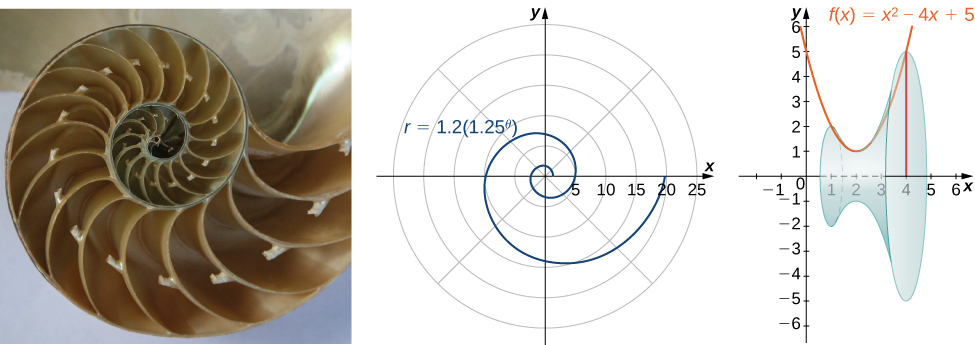
\includegraphics[width=\linewidth]{external/CNX_Calc_Figure_Preface_001_img.jpg}
\end{image}%
\begin{image}{0.25}{0.5}{0.25}%
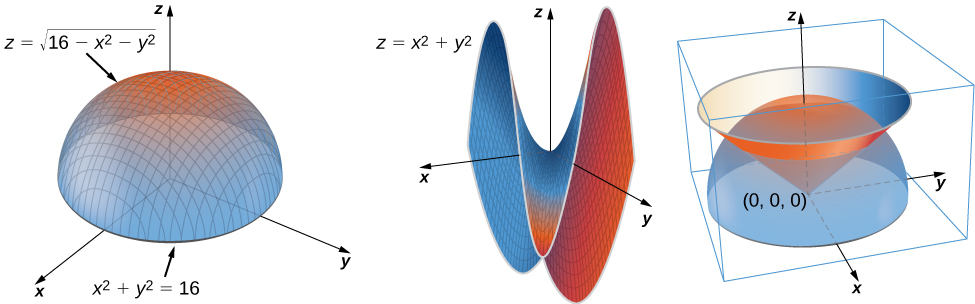
\includegraphics[width=\linewidth]{external/CNX_Calc_Figure_Preface_002_img.jpg}
\end{image}%
\end{subsectionptx}
\end{sectionptx}
%
%
\typeout{************************************************}
\typeout{Section 4 Additional resources}
\typeout{************************************************}
%
\begin{sectionptx}{Additional resources}{}{Additional resources}{}{}{g:section:idm1622763880}
%
%
\typeout{************************************************}
\typeout{Subsection 4.1 Student and instructor resources}
\typeout{************************************************}
%
\begin{subsectionptx}{Student and instructor resources}{}{Student and instructor resources}{}{}{g:subsection:idm1622741224}
We’ve compiled additional resources for both students and instructors, including Getting Started Guides, an instructor solution manual, and PowerPoint slides. Instructor resources require a verified instructor account, which can be requested on your OpenStax.org log-in. Take advantage of these resources to supplement your OpenStax book.%
\end{subsectionptx}
%
%
\typeout{************************************************}
\typeout{Subsection 4.2 Community Hubs}
\typeout{************************************************}
%
\begin{subsectionptx}{Community Hubs}{}{Community Hubs}{}{}{g:subsection:idm1622736488}
OpenStax partners with the Institute for the Study of Knowledge Management in Education (ISKME) to offer Community Hubs on OER Commons – a platform for instructors to share community-created resources that support OpenStax books, free of charge. Through our Community Hubs, instructors can upload their own materials or download resources to use in their own courses, including additional ancillaries, teaching material, multimedia, and relevant course content. We encourage instructors to join the hubs for the subjects most relevant to your teaching and research as an opportunity both to enrich your courses and to engage with other faculty.%
\par
To reach the Community Hubs, visit \href{www.oercommons.org/hubs/OpenStax}{www.oercommons.org\slash{}hubs\slash{}OpenStax}\footnote{\nolinkurl{www.oercommons.org/hubs/OpenStax}\label{g:fn:idm1622739432}}.%
\end{subsectionptx}
%
%
\typeout{************************************************}
\typeout{Subsection 4.3 Partner resources}
\typeout{************************************************}
%
\begin{subsectionptx}{Partner resources}{}{Partner resources}{}{}{g:subsection:idm1622737256}
OpenStax Partners are our allies in the mission to make high-quality learning materials affordable and accessible to students and instructors everywhere. Their tools integrate seamlessly with our OpenStax titles at a low cost. To access the partner resources for your text, visit your book page on OpenStax.org.%
\end{subsectionptx}
\end{sectionptx}
%
%
\typeout{************************************************}
\typeout{Section 5 About the authors}
\typeout{************************************************}
%
\begin{sectionptx}{About the authors}{}{About the authors}{}{}{g:section:idm1622742504}
%
%
\typeout{************************************************}
\typeout{Subsection 5.1 Senior contributing authors}
\typeout{************************************************}
%
\begin{subsectionptx}{Senior contributing authors}{}{Senior contributing authors}{}{}{g:subsection:idm1622731496}
\emph{Gilbert Strang, Massachusetts Institute of Technology} Dr. Strang received his PhD from UCLA in 1959 and has been teaching mathematics at MIT ever since. His Calculus online textbook is one of eleven that he has published and is the basis from which our final product has been derived and updated for today’s student. Strang is a decorated mathematician and past Rhodes Scholar at Oxford University.%
\par
\emph{Edwin “Jed” Herman, University of Wisconsin-Stevens Point} Dr. Herman earned a BS in Mathematics from Harvey Mudd College in 1985, an MA in Mathematics from UCLA in 1987, and a PhD in Mathematics from the University of Oregon in 1997. He is currently a Professor at the University of Wisconsin-Stevens Point. He has more than 20 years of experience teaching college mathematics, is a student research mentor, is experienced in course development\slash{}design, and is also an avid board game designer and player.%
\end{subsectionptx}
%
%
\typeout{************************************************}
\typeout{Subsection 5.2 Contributing authors}
\typeout{************************************************}
%
\begin{subsectionptx}{Contributing authors}{}{Contributing authors}{}{}{g:subsection:idm1622731368}
%
\begin{itemize}[label=\textbullet]
\item{}Catherine Abbott, Keuka College%
\item{}Nicoleta Virginia Bila, Fayetteville State University%
\item{}Sheri J. Boyd, Rollins College%
\item{}Joyati Debnath, Winona State University%
\item{}Valeree Falduto, Palm Beach State College%
\item{}Joseph Lakey, New Mexico State University%
\item{}Julie Levandosky, Framingham State University%
\item{}David McCune, William Jewell College%
\item{}Michelle Merriweather, Bronxville High School%
\item{}Kirsten R. Messer, Colorado State University - Pueblo%
\item{}Alfred K. Mulzet, Florida State College at Jacksonville%
\item{}William Radulovich (retired), Florida State College at Jacksonville%
\item{}Erica M. Rutter, Arizona State University%
\item{}David Smith, University of the Virgin Islands%
\item{}Elaine A. Terry, Saint Joseph’s University%
\item{}David Torain, Hampton University%
\end{itemize}
%
\end{subsectionptx}
%
%
\typeout{************************************************}
\typeout{Subsection 5.3 Reviewers}
\typeout{************************************************}
%
\begin{subsectionptx}{Reviewers}{}{Reviewers}{}{}{g:subsection:idm1622723432}
%
\begin{itemize}[label=\textbullet]
\item{}Marwan A. Abu-Sawwa, Florida State College at Jacksonville%
\item{}Kenneth J. Bernard, Virginia State University%
\item{}John Beyers, University of Maryland%
\item{}Charles Buehrle, Franklin \& Marshall College%
\item{}Matthew Cathey, Wofford College%
\item{}Michael Cohen, Hofstra University%
\item{}William DeSalazar, Broward County School System%
\item{}Murray Eisenberg, University of Massachusetts Amherst%
\item{}Kristyanna Erickson, Cecil College%
\item{}Tiernan Fogarty, Oregon Institute of Technology%
\item{}David French, Tidewater Community College%
\item{}Marilyn Gloyer, Virginia Commonwealth University%
\item{}Shawna Haider, Salt Lake Community College%
\item{}Lance Hemlow, Raritan Valley Community College%
\item{}Jerry Jared, The Blue Ridge School%
\item{}Peter Jipsen, Chapman University%
\item{}David Johnson, Lehigh University%
\item{}M.R. Khadivi, Jackson State University%
\item{}Robert J. Krueger, Concordia University%
\item{}Tor A. Kwembe, Jackson State University%
\item{}Jean-Marie Magnier, Springfield Technical Community College%
\item{}Cheryl Chute Miller, SUNY Potsdam%
\item{}Bagisa Mukherjee, Penn State University, Worthington Scranton Campus%
\item{}Kasso Okoudjou, University of Maryland College Park%
\item{}Peter Olszewski, Penn State Erie, The Behrend College%
\item{}Steven Purtee, Valencia College%
\item{}Alice Ramos, Bethel College%
\item{}Doug Shaw, University of Northern Iowa%
\item{}Hussain Elalaoui-Talibi, Tuskegee University%
\item{}Jeffrey Taub, Maine Maritime Academy%
\item{}William Thistleton, SUNY Polytechnic Institute%
\item{}A. David Trubatch, Montclair State University%
\item{}Carmen Wright, Jackson State University%
\item{}Zhenbu Zhang, Jackson State University%
\end{itemize}
%
\end{subsectionptx}
\end{sectionptx}
\end{preface}
%
%
\typeout{************************************************}
\typeout{Preface  Preface: Business Calculus Custom Edition}
\typeout{************************************************}
%
\begin{preface}{Preface: Business Calculus Custom Edition}{}{Preface: Business Calculus Custom Edition}{}{}{g:preface:idm1622769640}
This book has been adapted by Katie Hall and Kim Savinon at University of Connecticut to be used for a Business Calculus course.%
\end{preface}
%% begin: table of contents
%% Adjust Table of Contents
\setcounter{tocdepth}{1}
\renewcommand*\contentsname{Contents}
\tableofcontents
%% end:   table of contents
\mainmatter
%
%
\typeout{************************************************}
\typeout{Chapter 1 Functions and Graphs}
\typeout{************************************************}
%
\begin{chapterptx}{Functions and Graphs}{}{Functions and Graphs}{}{}{x:chapter:ch_first}
\begin{introduction}{}%
\begin{figureptx}{A portion of the San Andreas Fault in California. Major faults like this are the sites of most of the strongest earthquakes ever recorded. (credit: modification of work by Robb Hannawacker, NPS)}{g:figure:idm1622711144}{}%
\begin{image}{0.25}{0.5}{0.25}%
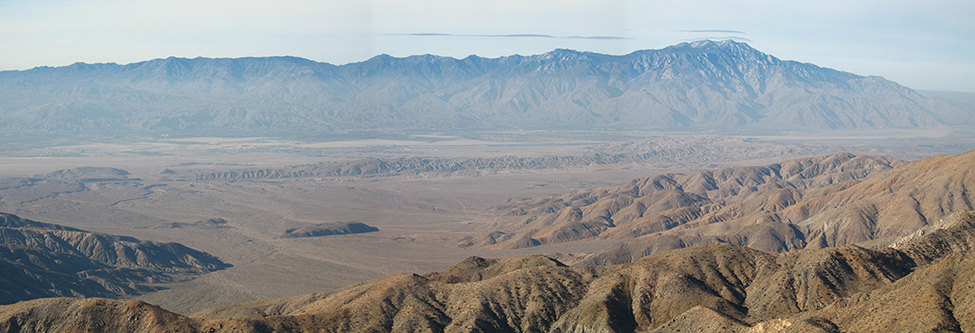
\includegraphics[width=\linewidth]{external/CNX_Calc_Figure_01_00_003.jpg}
\end{image}%
\tcblower
\end{figureptx}%
%
\par
In the past few years, major earthquakes have occurred in several countries around the world. In January 2010, an earthquake of magnitude 7.3 hit Haiti. A magnitude 9 earthquake shook northeastern Japan in March 2011. In April 2014, an 8.2-magnitude earthquake struck off the coast of northern Chile. What do these numbers mean? In particular, how does a magnitude 9 earthquake compare with an earthquake of magnitude 8.2? Or 7.3? Later in this chapter, we show how logarithmic functions are used to compare the relative intensity of two earthquakes based on the magnitude of each earthquake.%
\par
Calculus is the mathematics that describes changes in functions. In this chapter, we review all the functions necessary to study calculus. We define polynomial, rational, trigonometric, exponential, and logarithmic functions. We review how to evaluate these functions, and we show the properties of their graphs. We provide examples of equations with terms involving these functions and illustrate the algebraic techniques necessary to solve them. In short, this chapter provides the foundation for the material to come. It is essential to be familiar and comfortable with these ideas before proceeding to the formal introduction of calculus in the next chapter.%
\par
This book is a custom edition based on OpenStax Calculus Volume 1. You can download the original for free at https:\slash{}\slash{}openstax.org\slash{}details\slash{}books\slash{}calculus-volume-1.%
\end{introduction}%
%
%
\typeout{************************************************}
\typeout{Section 1.1 Review of Functions}
\typeout{************************************************}
%
\begin{sectionptx}{Review of Functions}{}{Review of Functions}{}{}{x:section:sec_Ch1Sec1}
\begin{introduction}{Learning Objectives.}%
%
\begin{enumerate}
\item{}Use functional notation to evaluate a function.%
\item{}Determine the domain and range of a function.%
\item{}Draw the graph of a function.%
\item{}Find the zeros of a function.%
\item{}Recognize a function from a table of values.%
\item{}Make new functions from two or more given functions.%
\item{}Describe the symmetry properties of a function.%
\end{enumerate}
In this section, we provide a formal definition of a function and examine several ways in which functions are represented—namely, through tables, formulas, and graphs. We study formal notation and terms related to functions. We also define composition of functions and symmetry properties. Most of this material will be a review for you, but it serves as a handy reference to remind you of some of the algebraic techniques useful for working with functions.%
\end{introduction}%
%
%
\typeout{************************************************}
\typeout{Subsection 1.1.1 Functions}
\typeout{************************************************}
%
\begin{subsectionptx}{Functions}{}{Functions}{}{}{x:subsection:subsec_Ch1Sec1Ss1}
Given two sets \(A\) and \(B\), a set with elements that are ordered pairs \((x,y) \) where \(x\) is an element of \(A\) and \(y\) is an element of \(B\), is a relation from \(A\)   to \(B\). A relation from \(A\) to \(B\) defines a relationship between those two sets. A function is a special type of relation in which each element of the first set is related to exactly one element of the second set. The element of the first set is called the \emph{input}; the element of the second set is called the \emph{output}. Functions are used all the time in mathematics to describe relationships between two sets. For any function, when we know the input, the output is determined, so we say that the output is a function of the input. For example, the area of a square is determined by its side length, so we say that the area (the output) is a function of its side length (the input). The velocity of a ball thrown in the air can be described as a function of the amount of time the ball is in the air. The cost of mailing a package is a function of the weight of the package. Since functions have so many uses, it is important to have precise definitions and terminology to study them.%
\begin{definition}{}{g:definition:idm1622701672}%
A \terminology{function}\(f\) consists of a set of inputs, a set of outputs, and a rule for assigning each input to exactly one output. The set of inputs is called the \terminology{domain} of the function. The set of outputs is called the \terminology{range} of the function.\end{definition}
For example, consider the function \(f\), where the domain is the set of all real numbers and the rule is to square the input. Then, the input \(x=3\) is assigned to the output \(3^2=9\). Since every nonnegative real number has a real-value square root, every nonnegative number is an element of the range of this function. Since there is no real number with a square that is negative, the negative real numbers are not elements of the range. We conclude that the range is the set of nonnegative real numbers. For a general function \(f\) with domain \(D\), we often use \(x\) to denote the input and \(y\) to denote the output associated with \(x\). When doing so, we refer to \(x\) as the \terminology{independent variable} and \(y\) as the \terminology{dependent variable}, because it depends on \(x\). Using function notation, we write \(y=f(x)\) and we read this equation as “\(y\) equals \(f\) of \(x\).” For the squaring function described earlier, we write \(f(x)=x^2.\)%
\par
The concept of a function can be visualized using \hyperref[x:figure:CNX_Calc_Figure_01_01_001]{Figure~{\xreffont\ref{x:figure:CNX_Calc_Figure_01_01_001}}}, \hyperref[x:figure:CNX_Calc_Figure_01_01_002]{Figure~{\xreffont\ref{x:figure:CNX_Calc_Figure_01_01_002}}} and \hyperref[x:figure:CNX_Calc_Figure_01_01_003]{Figures~{\xreffont\ref{x:figure:CNX_Calc_Figure_01_01_003}}}.%
\begin{figureptx}{A function can be visualized as an input\slash{}output device.}{x:figure:CNX_Calc_Figure_01_01_001}{}%
\begin{image}{0.25}{0.5}{0.25}%
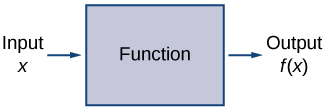
\includegraphics[width=\linewidth]{external/CNX_Calc_Figure_01_01_001.jpg}
\end{image}%
\tcblower
\end{figureptx}%
\begin{figureptx}{A function maps every element in the domain to exactly one element in the range. Although each input can be sent to only one output, two different inputs can be sent to the same output.}{x:figure:CNX_Calc_Figure_01_01_002}{}%
\begin{image}{0.25}{0.5}{0.25}%
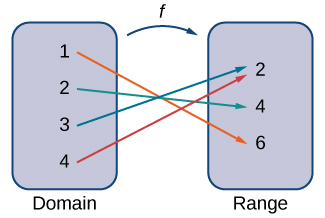
\includegraphics[width=\linewidth]{external/CNX_Calc_Figure_01_01_002.jpg}
\end{image}%
\tcblower
\end{figureptx}%
\begin{figureptx}{In this case, a graph of a function f has a domain of \textbraceleft{}1,2,3\textbraceright{} and a range of \textbraceleft{}1,2\textbraceright{}. The independent variable is x and the dependent variable is y.}{x:figure:CNX_Calc_Figure_01_01_003}{}%
\begin{image}{0.25}{0.5}{0.25}%
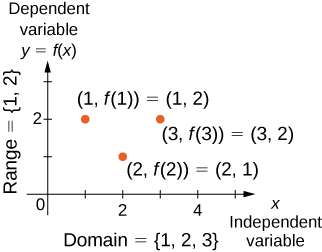
\includegraphics[width=\linewidth]{external/CNX_Calc_Figure_01_01_003.jpg}
\end{image}%
\tcblower
\end{figureptx}%
\begin{note}{}{g:note:idm1622682984}%
Visit this \href{http://www.openstax.org/l/grapherrors}{applet link}\footnotemark{} to see more about graphs of functions.%
\end{note}
\footnotetext[1]{\nolinkurl{http://www.openstax.org/l/grapherrors}\label{g:fn:idm1622682600}}%
We can also visualize a function by plotting points \((x,y)\) in the coordinate plane where \(y=f(x)\). The \terminology{graph of a function} is the set of all these points. For example, consider the function \(f\) where the domain is the set \(D=\{1,2,3\}\) and the rule is \(f(x)=3-x.\) In \hyperref[x:figure:CNX_Calc_Figure_01_01_004]{Figure~{\xreffont\ref{x:figure:CNX_Calc_Figure_01_01_004}}}, we plot a graph of this function.%
\begin{figureptx}{Here we see a graph of the function \(f\) with domain \(\{1,2,3\}\) and rule \(f(x)=3-x.\) The graph consists of the points \((x,f(x))\) for all \(x\) in the domain.}{x:figure:CNX_Calc_Figure_01_01_004}{}%
\begin{image}{0.25}{0.5}{0.25}%
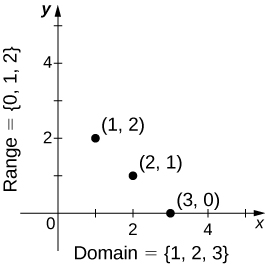
\includegraphics[width=\linewidth]{external/CNX_Calc_Figure_01_01_004.jpg}
\end{image}%
\tcblower
\end{figureptx}%
Every function has a domain. However, sometimes a function is described by an equation, as in \(f(x)=x^2,\) with no specific domain given. In this case, the domain is taken to be the set of all real numbers \(x\) for which \(f(x)\) is a real number. For example, since any real number can be squared, if no other domain is specified, we consider the domain of \(f(x)=x^2\) to be the set of all real numbers. On the other hand, the square root function \(f(x)=\sqrt{x}\) only gives a real output if \(x\) is nonnegative. Therefore, the domain of the function \(f(x)=\sqrt{x}\) is the set of nonnegative real numbers, sometimes called the \terminology{natural domain}.%
\par
For the functions \(f(x)=x^2\) and \(f(x)=\sqrt{x},\) the domains are sets with an infinite number of elements. Clearly we cannot list all these elements. When describing a set with an infinite number of elements, it is often helpful to use set-builder or interval notation. When using set-builder notation to describe a subset of all real numbers, denoted \(\mathbb{R}],\) we write%
%
\begin{equation*}
\{x|x \text{ has some property} \}.
\end{equation*}
We read this as the set of real numbers \(x\) such that \(x\) has some property. For example, if we were interested in the set of real numbers that are greater than one but less than five, we could denote this set using set-builder notation by writing%
%
\begin{equation*}
\{x | 1 < x < 5 \}.
\end{equation*}
A set such as this, which contains all numbers greater than \(a\) and less than \(b,\) can also be denoted using the \terminology{interval notation} \((a,b).\) Therefore,%
\((1,5)=\{x| 1\leq  x \leq  5\}.\)The numbers \(1\) and \(5\) are called the \terminology{endpoints} of this set. If we want to consider the set that includes the endpoints, we would denote this set by writing%
%
\begin{equation*}
[1,5]=\{x|1\leq  x\leq 5\}.
\end{equation*}
We can use similar notation if we want to include one of the endpoints, but not the other. To denote the set of nonnegative real numbers, we would use the set-builder notation%
%
\begin{equation*}
\{x|0\leq  x\}.
\end{equation*}
The smallest number in this set is zero, but this set does not have a largest number. Using interval notation, we would use the symbol \(\infty ,\) which refers to positive infinity, and we would write the set as%
%
\begin{equation*}
[0,\infty)=\{x|0 \leq  x\}.
\end{equation*}
It is important to note that \(\infty\) is not a real number. It is used symbolically here to indicate that this set includes all real numbers greater than or equal to zero. Similarly, if we wanted to describe the set of all nonpositive numbers, we could write%
%
\begin{equation*}
(-\infty,0]=\{x|x \leq  0\}.
\end{equation*}
Here, the notation \(-\infty\) refers to negative infinity, and it indicates that we are including all numbers less than or equal to zero, no matter how small. The set%
%
\begin{equation*}
(-\infty,\infty)=\{x|x \text{ is any real number }\}
\end{equation*}
refers to the set of all real numbers.%
\par
Some functions are defined using different equations for different parts of their domain. These types of functions are known as \terminology{piecewise-defined functions}. For example, suppose we want to define a function \(f\) with a domain that is the set of all real numbers such that \(f(x)=3x+1\) for \(x \geq 2\) and \(f(x)=x^2\) for \(x < 2.\) We denote this function by writing%
%
\begin{equation*}
f(x)=\begin{cases} 3x+1 \amp x \geq 2 \\ x^2 \amp x < 2 .\end{cases}
\end{equation*}
When evaluating this function for an input \(x,\) the equation to use depends on whether \(x \geq 2\) or \(x < 2.\) For example, since \(5 \ge 2,\) we use the fact that \(f(x)=3x+1\) for \(x \geq 2\) and see that \(f(5)=3(5)+1=16.\) On the other hand, for \(x=-1,\) we use the fact that \(f(x)=x^2\) for \(x < 2\) and see that \(f(-1)=1.\)%
\begin{example}{Evaluating Functions.}{g:example:idm1622656360}%
For the function \(f(x)=3x^2+2x-1,\) evaluate%
%
\begin{enumerate}
\item{}\(\displaystyle f(-2)\)%
\item{}\(\displaystyle f(\sqrt{2})\)%
\item{}\(\displaystyle f(a+h)\)%
\end{enumerate}
\par\smallskip%
\noindent\textbf{\blocktitlefont Solution}.\hypertarget{g:solution:idm1622649576}{}\quad{}Substitute the given value for \(x \) in the formula for \(f(x).\)%
%
\begin{enumerate}
\item{}\(\displaystyle f(-2)=3(-2)^2+2(-2)-1=12-4-1=7\)%
\item{}\(\displaystyle f(\sqrt{2})=3(\sqrt{2})^2+2\sqrt{2}-1=6+2\sqrt{2}-1=5+2\sqrt{2}\)%
\item{}%
\begin{align*}
f(a+h)=3(a+h)^2+2(a+h)-1 \amp =3(a^2+2ah+h^2)+2a+2h-1\\
\amp =3a^2+6ah+3h^2+2a+2h-1
\end{align*}
%
\end{enumerate}
\end{example}
\begin{inlineexercise}{}{g:exercise:idm1622645352}%
For \(f(x)=x^2-3x+5,\) evaluate \(f(1)\) and \(f(a+h).\)%
\par\smallskip%
\noindent\textbf{\blocktitlefont Hint}.\hypertarget{g:hint:idm1622646888}{}\quad{}Substitute \(1\) and \(a+h\) for \(x\) in the formula for \(f(x).\)%
\par\smallskip%
\noindent\textbf{\blocktitlefont Solution}.\hypertarget{g:solution:idm1622644456}{}\quad{}\(f(1)=3\) and \(f(a+h)=a^2+2ah+h^2-3a-3h+5\)%
\end{inlineexercise}%
\begin{example}{Finding Domain and Range.}{g:example:idm1622644840}%
For each of the following functions, determine the a. domain and b. range.%
%
\begin{enumerate}
\item{}\(\displaystyle f(x)=(x-4)^2+5\)%
\item{}\(\displaystyle f(x)=\sqrt{3x+2}-1\)%
\item{}\(\displaystyle f(x)=\frac{3}{x-2}\)%
\end{enumerate}
\par\smallskip%
\noindent\textbf{\blocktitlefont Solution}.\hypertarget{g:solution:idm1622636392}{}\quad{}%
\begin{enumerate}
\item{}Consider \(f(x)=(x-4)^2+5.\)%
%
\begin{enumerate}
\item{}Since \(f(x)=(x-4)^2+5\) is a real number for any real number \(x,\) the domain of \(f\) is the interval \((-\infty, \infty).\)%
\item{}Since \((x-4)^2 \geq 0,\) we know \(f(x)=(x-4)^2+5 \geq 5.\) Therefore, the range must be a subset of \(\{y|y \geq 5\}.\) To show that every element in this set is in the range, we need to show that for a given \(y\) in that set, there is a real number \(x\) such that \(f(x)=(x-4)^2+5=y.\) Solving this equation for \(x,\) we see that we need \(x\) such that%
\begin{equation*}
(x-4)^2=y-5.
\end{equation*}
This equation is satisfied as long as there exists a real number \(x\) such that%
\begin{equation*}
x-4= \pm \sqrt{y-5}.
\end{equation*}
Since \(y \geq 5,\) the square root is well-defined. We conclude that for \(x=4 \pm \sqrt{y-5},f(x)=y,\) and therefore the range is \(\{y|y \geq 5\}.\)%
\end{enumerate}
\item{}Consider \(f(x)=\sqrt{3x+2}-1.\)%
%
\begin{enumerate}
\item{}To find the domain of \(f,\) we need the expression \(3x+2 \geq 0.\) Solving this inequality, we conclude that the domain is \(\{x|x\geq-2/3\}.\)%
\item{}To find the range of \(f,\) we note that since \(\sqrt{3x+2}\geq 0,f(x)=\sqrt{3x+2}-1\geq -1.\) Therefore, the range of \(f\) must be a subset of the set \(\{y|y\geq-1\}.\) To show that every element in this set is in the range of \(f,\) we need to show that for all \(y\) in this set, there exists a real number \(x\) in the domain such that \(f(x)=y.\) Let \(y\geq-1.\) Then, \(f(x)=y\) if and only if%
\begin{equation*}
\sqrt{3x+2}-1=y.
\end{equation*}
Solving this equation for \(x,\) we see that \(x\) must solve the equation%
\begin{equation*}
\sqrt{3x+2}=y+1.
\end{equation*}
Since \(y\geq-1,\) such an \(x\) could exist. Squaring both sides of this equation, we have%
\begin{equation*}
3x+2=(y+1)^2.
\end{equation*}
Therefore, we need%
\begin{equation*}
3x=(y+1)^2-2,
\end{equation*}
which implies%
\begin{equation*}
x=\frac{1}{3}(y+1)^2-\frac{2}{3}.
\end{equation*}
We just need to verify that \(x\) is in the domain of \(f.\) Since the domain of \(f\) consists of all real numbers greater than or equal to \(-2/3,\) and%
\begin{equation*}
\frac{1}{3}(y+1)^2-\frac{2}{3}\geq -\frac{2}{3},
\end{equation*}
there does exist an \(x\) in the domain of \(f.\) We conclude that the range of \(f\) is \(\{y|y\geq-1\}.\)%
\end{enumerate}
\item{}Consider \(f(x)=3/(x-2).\)%
\begin{enumerate}
\item{}Since \(3/(x-2)\) is defined when the denominator is nonzero, the domain is \(\{x|x \neq 2\}.\)%
\item{}To find the range of \(f,\) we need to find the values of \(y\) such that there exists a real number \(x\) in the domain with the property that%
\begin{equation*}
\frac{3}{x-2}=y.
\end{equation*}
Solving this equation for \(x,\) we find that%
\begin{equation*}
x=\frac{3}{y}+2.
\end{equation*}
Therefore, as long as \(y\neq 0,\) there exists a real number \(x\) in the domain such that \(f(x)=y.\) Thus, the range is \(\{y|y \neq 0\}.\)%
\end{enumerate}
%
\end{enumerate}
\end{example}
\begin{inlineexercise}{}{g:exercise:idm1622605160}%
Find the domain and range for \(f(x)=\sqrt{4-2x}+5.\)%
\par\smallskip%
\noindent\textbf{\blocktitlefont Hint}.\hypertarget{g:hint:idm1622606440}{}\quad{}Use \(4-2x\geq0.\)%
\par\smallskip%
\noindent\textbf{\blocktitlefont Solution}.\hypertarget{g:solution:idm1622605800}{}\quad{}Domain = \(\{x|x \leq  2\},\) range = \(\{y|y\geq 5\}\)%
\end{inlineexercise}%
\end{subsectionptx}
%
%
\typeout{************************************************}
\typeout{Subsection 1.1.2 Representing Functions}
\typeout{************************************************}
%
\begin{subsectionptx}{Representing Functions}{}{Representing Functions}{}{}{g:subsection:idm1622604264}
\begin{introduction}{}%
Typically, a function is represented using one or more of the following tools:%
%
\begin{itemize}[label=\textbullet]
\item{}A table%
\item{}A graph%
\item{}A formula%
\end{itemize}
We can identify a function in each form, but we can also use them together. For instance, we can plot on a graph the values from a table or create a table from a formula.%
\end{introduction}%
%
%
\typeout{************************************************}
\typeout{Subsubsection 1.1.2.1 Tables}
\typeout{************************************************}
%
\begin{subsubsectionptx}{Tables}{}{Tables}{}{}{g:subsubsection:idm1622600552}
Functions described using a \terminology{table of values} arise frequently in real-world applications. Consider the following simple example. We can describe temperature on a given day as a function of time of day. Suppose we record the temperature every hour for a 24-hour period starting at midnight. We let our input variable \(x\) be the time after midnight, measured in hours, and the output variable \(y\) be the temperature \(x\) hours after midnight, measured in degrees Fahrenheit. We record our data in \hyperref[x:table:fs-id1170572114646]{Table~{\xreffont\ref{x:table:fs-id1170572114646}}}.%
\begin{tableptx}{\textbf{Temperature as a Function of Time of Day}}{x:table:fs-id1170572114646}{}%
\centering%
{\tabularfont%
\begin{tabular}{llll}
\multicolumn{1}{c}{\textbf{Hours after Midnight}}&\multicolumn{1}{c}{\textbf{Temperature  (\(^\circ\)F)}}&\multicolumn{1}{c}{\textbf{Hours after Midnight}}&\multicolumn{1}{c}{\textbf{Temperature  (\(^\circ\)F)}}\tabularnewline[0pt]
0&58&12&84\tabularnewline[0pt]
1&54&13&85\tabularnewline[0pt]
2&53&14&85\tabularnewline[0pt]
3&52&15&83\tabularnewline[0pt]
4&52&16&82\tabularnewline[0pt]
5&55&17&80\tabularnewline[0pt]
6&60&18&77\tabularnewline[0pt]
7&64&19&74\tabularnewline[0pt]
8&72&20&69\tabularnewline[0pt]
9&75&21&65\tabularnewline[0pt]
10&78&22&60\tabularnewline[0pt]
11&80&23&58
\end{tabular}
}%
\end{tableptx}%
We can see from the table that temperature is a function of time, and the temperature decreases, then increases, and then decreases again. However, we cannot get a clear picture of the behavior of the function without graphing it.%
\end{subsubsectionptx}
%
%
\typeout{************************************************}
\typeout{Subsubsection 1.1.2.2 Graphs}
\typeout{************************************************}
%
\begin{subsubsectionptx}{Graphs}{}{Graphs}{}{}{g:subsubsection:idm1622573032}
Given a function \(f\) described by a table, we can provide a visual picture of the function in the form of a graph. Graphing the temperatures listed in \hyperref[x:table:fs-id1170572114646]{Table~{\xreffont\ref{x:table:fs-id1170572114646}}} can give us a better idea of their fluctuation throughout the day. \hyperref[x:figure:CNX_Calc_Figure_01_01_005]{Figure~{\xreffont\ref{x:figure:CNX_Calc_Figure_01_01_005}}} shows the plot of the temperature function.%
\begin{figureptx}{The graph of the data from \hyperref[x:table:fs-id1170572114646]{Table~{\xreffont\ref{x:table:fs-id1170572114646}}} shows temperature as a function of time.}{x:figure:CNX_Calc_Figure_01_01_005}{}%
\begin{image}{0.25}{0.5}{0.25}%
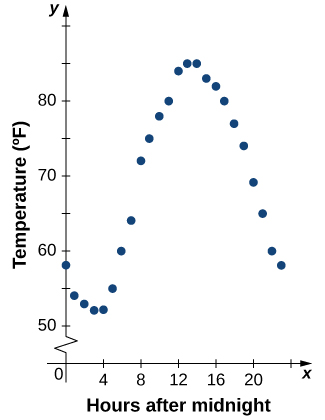
\includegraphics[width=\linewidth]{external/CNX_Calc_Figure_01_01_005.jpg}
\end{image}%
\tcblower
\end{figureptx}%
From the points plotted on the graph in \hyperref[x:figure:CNX_Calc_Figure_01_01_005]{Figure~{\xreffont\ref{x:figure:CNX_Calc_Figure_01_01_005}}}, we can visualize the general shape of the graph. It is often useful to connect the dots in the graph, which represent the data from the table. In this example, although we cannot make any definitive conclusion regarding what the temperature was at any time for which the temperature was not recorded, given the number of data points collected and the pattern in these points, it is reasonable to suspect that the temperatures at other times followed a similar pattern, as we can see in \hyperref[x:figure:CNX_Calc_Figure_01_01_014]{Figure~{\xreffont\ref{x:figure:CNX_Calc_Figure_01_01_014}}}.%
\begin{figureptx}{Connecting the dots in  \hyperref[x:figure:CNX_Calc_Figure_01_01_005]{Figure~{\xreffont\ref{x:figure:CNX_Calc_Figure_01_01_005}}}  shows the general pattern of the data.}{x:figure:CNX_Calc_Figure_01_01_014}{}%
\begin{image}{0}{1}{0}%
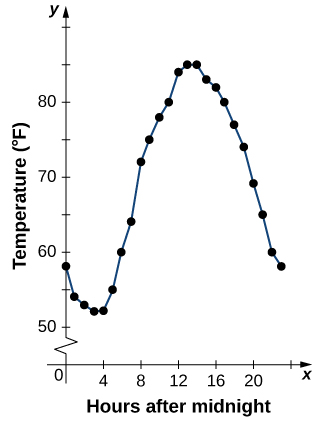
\includegraphics[width=\linewidth]{external/CNX_Calc_Figure_01_01_014.jpg}
\end{image}%
\tcblower
\end{figureptx}%
\end{subsubsectionptx}
%
%
\typeout{************************************************}
\typeout{Subsubsection 1.1.2.3 Algebraic Formulas}
\typeout{************************************************}
%
\begin{subsubsectionptx}{Algebraic Formulas}{}{Algebraic Formulas}{}{}{g:subsubsection:idm1622566632}
Sometimes we are not given the values of a function in table form, rather we are given the values in an explicit formula. Formulas arise in many applications. For example, the area of a circle of radius \(r\) is given by the formula \(A(r)=\pi r^2.\) When an object is thrown upward from the ground with an initial velocity \(v_0\) ft\slash{}s, its height above the ground from the time it is thrown until it hits the ground is given by the formula \(s(t)=-16t^2+v_0 t.\) When \(P\) dollars are invested in an account at an annual interest rate \(r\) compounded continuously, the amount of money after \(t\) years is given by the formula \(A(t)=Pe^{rt}.\) Algebraic formulas are important tools to calculate function values. Often we also represent these functions visually in graph form.%
\par
Given an algebraic formula for a function \(f,\) the graph of \(f\) is the set of points \((x,f(x)),\) where \(x\) is in the domain of \(f\) and \(f(x)\) is in the range. To graph a function given by a formula, it is helpful to begin by using the formula to create a table of inputs and outputs. If the domain of \(f\) consists of an infinite number of values, we cannot list all of them, but because listing some of the inputs and outputs can be very useful, it is often a good way to begin.%
\par
When creating a table of inputs and outputs, we typically check to determine whether zero is an output. Those values of \(x\) where \(f(x)=0\) are called the \terminology{zeros of a function}. For example, the zeros of \(f(x)=x^2-4\) are \(x=±2.\) The zeros determine where the graph of \(f\) intersects the \(x\)-axis, which gives us more information about the shape of the graph of the function. The graph of a function may never intersect the x-axis, or it may intersect multiple (or even infinitely many) times.%
\par
Another point of interest is the \(y\)-intercept, if it exists. The \(y\)-intercept is given by \((0,f(0)).\)%
\par
Since a function has exactly one output for each input, the graph of a function can have, at most, one \(y\)-intercept. If \(x=0\) is in the domain of a function \(f,\) then \(f\) has exactly one \(y\)-intercept. If \(x=0\) is not in the domain of \(f,\) then \(f\) has no \(y\)-intercept. Similarly, for any real number \(c,\) if \(c\) is in the domain of \(f,\) there is exactly one output \(f(c),\) and the line \(x=c\) intersects the graph of \(f\) exactly once. On the other hand, if \(c\) is not in the domain of \(f,f(c)\) is not defined and the line \(x=c\) does not intersect the graph of \(f.\) This property is summarized in the \terminology{vertical line test}.%
\begin{note}{Rule: Vertical Line Test.}{g:note:idm1622545640}%
Given a function \(f,\) every vertical line that may be drawn intersects the graph of \(f\) no more than once. If any vertical line intersects a set of points more than once, the set of points does not represent a function.%
\end{note}
We can use this test to determine whether a set of plotted points represents the graph of a function (\hyperref[x:figure:CNX_Calc_Figure_01_01_006]{Figure~{\xreffont\ref{x:figure:CNX_Calc_Figure_01_01_006}}} ).%
\begin{figureptx}{(a) The set of plotted points represents the graph of a function because every vertical line intersects the set of points, at most, once. (b) The set of plotted points does not represent the graph of a function because some vertical lines intersect the set of points more than once.}{x:figure:CNX_Calc_Figure_01_01_006}{}%
\begin{image}{0}{1}{0}%
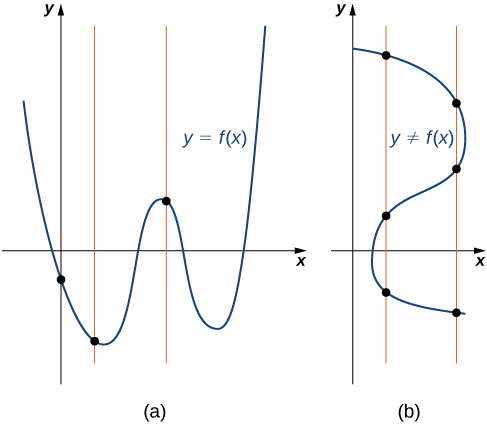
\includegraphics[width=\linewidth]{external/CNX_Calc_Figure_01_01_006.jpg}
\end{image}%
\tcblower
\end{figureptx}%
\end{subsubsectionptx}
\begin{example}{Finding Zeros and \(y\)-Intercepts of a Function.}{g:example:idm1622600680}%
Consider the function \(f(x)=-4x+2.\)%
%
\begin{enumerate}
\item{}Find all zeros of \(f.\)%
\item{}Find the \(y\)-intercept (if any).%
\item{}Sketch a graph of \(f.\)%
\end{enumerate}
\par\smallskip%
\noindent\textbf{\blocktitlefont Solution}.\hypertarget{g:solution:idm1622537704}{}\quad{}%
\begin{enumerate}
\item{}To find the zeros, solve \(f(x)=-4x+2=0.\) We discover that \(f\) has one zero at \(x=1/2.\)%
\item{}The \(y\)-intercept is given by \((0,f(0))=(0,2).\)%
\item{}Given that \(f\) is a linear function of the form \(f(x)=mx+b\) that passes through the points \((1/2,0)\) and \((0,2),\) we can sketch the graph of \(f\) (\hyperref[x:figure:CNX_Calc_Figure_01_01_007]{Figure~{\xreffont\ref{x:figure:CNX_Calc_Figure_01_01_007}}}). \begin{figureptx}{The function \(f(x)=-4x+2\) is a line with \(x\)-intercept \((1/2,0)\) and \(y\)-intercept \((0,2).\)}{x:figure:CNX_Calc_Figure_01_01_007}{}%
\begin{image}{0}{1}{0}%
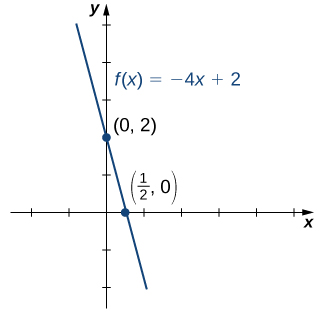
\includegraphics[width=\linewidth]{external/CNX_Calc_Figure_01_01_007.jpg}
\end{image}%
\tcblower
\end{figureptx}%
%
\end{enumerate}
\end{example}
\begin{example}{Using Zeros and \(y\)-Intercepts to Sketch a Graph.}{g:example:idm1622529640}%
Consider the function \(f(x)=\sqrt{x+3}+1.\)%
%
\begin{enumerate}
\item{}Find all zeros of \(f.\)%
\item{}Find the \(y\)-intercept (if any).%
\item{}Sketch a graph of \(f.\)%
\end{enumerate}
\par\smallskip%
\noindent\textbf{\blocktitlefont Solution}.\hypertarget{g:solution:idm1622524264}{}\quad{}%
\begin{enumerate}
\item{}To find the zeros, solve \(\sqrt{x+3}+1=0.\) This equation implies \(\sqrt{x+3}=-1.\) Since \(\sqrt{x+3}\geq 0\) for all \(x,\) this equation has no solutions, and therefore \(f\) has no zeros.%
\item{}The \(y\)-intercept is given by \((0,f(0))=(0,\sqrt{3}+1).\)%
\item{}To graph this function, we make a table of values. Since we need \(x+3 \geq 0,\) we need to choose values of \(x\geq -3.\) We choose values that make the square-root function easy to evaluate. \begin{tableptx}{\textbf{}}{x:table:fs-id1170572247842}{}%
\centering%
{\tabularfont%
\begin{tabular}{llll}
\multicolumn{1}{c}{\(x\)}&\multicolumn{1}{c}{\(-3\)}&\multicolumn{1}{c}{\(-2\)}&\multicolumn{1}{c}{\(1\)}\tabularnewline[0pt]
\multicolumn{1}{c}{\(f(x)\)}&\multicolumn{1}{c}{\(1\)}&\multicolumn{1}{c}{\(2\)}&\multicolumn{1}{c}{\(3\)}
\end{tabular}
}%
\end{tableptx}%
%
\end{enumerate}
Making use of the table and knowing that, since the function is a square root, the graph of \(f\) should be similar to the graph of \(y=\sqrt{x},\) we sketch the graph (\hyperref[x:figure:CNX_Calc_Figure_01_01_008]{Figure~{\xreffont\ref{x:figure:CNX_Calc_Figure_01_01_008}}}).%
\begin{figureptx}{The graph of \(f(x)=\sqrt{x+3}+1\) has a \(y\)-intercept but no \(x\)-intercepts.}{x:figure:CNX_Calc_Figure_01_01_008}{}%
\begin{image}{0}{1}{0}%
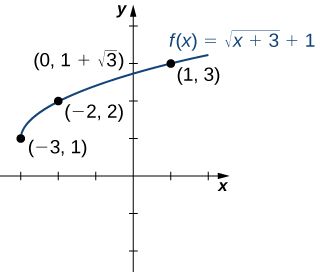
\includegraphics[width=\linewidth]{external/CNX_Calc_Figure_01_01_008.jpg}
\end{image}%
\tcblower
\end{figureptx}%
\end{example}
\begin{inlineexercise}{}{g:exercise:idm1622704744}%
Find the zeros of \(f(x)=x^3-5x^2+6x.\)%
\par\smallskip%
\noindent\textbf{\blocktitlefont Hint}.\hypertarget{g:hint:idm1622507624}{}\quad{}Factor the polynomial.%
\par\smallskip%
\noindent\textbf{\blocktitlefont Solution}.\hypertarget{g:solution:idm1622509928}{}\quad{}\(x=0,2,3\)%
\end{inlineexercise}%
\begin{example}{Finding the Height of a Free-Falling Object.}{g:example:idm1622508648}%
If a ball is dropped from a height of \(100\) ft, its height \(s\) at time \(t\) is given by the function \(s(t)=-16t^2+100,\) where \(s\) is measured in feet and \(t\) is measured in seconds. The domain is restricted to the interval \([0,c],\) where \(t=0\) is the time when the ball is dropped and \(t=c\) is the time when the ball hits the ground.%
%
\begin{enumerate}
\item{}Create a table showing the height \(s(t)\) when \(t=0,0.5,1,1.5,2, \) and \(2.5.\) Using the data from the table, determine the domain for this function. That is, find the time \(c\) when the ball hits the ground.%
\item{}Sketch a graph of \(s.\)%
\end{enumerate}
\par\smallskip%
\noindent\textbf{\blocktitlefont Solution}.\hypertarget{g:solution:idm1622462824}{}\quad{}%
\begin{enumerate}
\item{}\begin{tableptx}{\textbf{Height \(s\) as a Function of Time \(t\)}}{g:table:idm1622463720}{}%
\centering%
{\tabularfont%
\begin{tabular}{lllllll}
\multicolumn{1}{c}{\(t\)}&\multicolumn{1}{c}{\(0\)}&\multicolumn{1}{c}{\(0.5\)}&\multicolumn{1}{c}{\(1\)}&\multicolumn{1}{c}{\(1.5\)}&\multicolumn{1}{c}{\(2\)}&\multicolumn{1}{c}{\(2.5\)}\tabularnewline[0pt]
\multicolumn{1}{c}{\(s(t)\)}&\multicolumn{1}{c}{\(100\)}&\multicolumn{1}{c}{\(96\)}&\multicolumn{1}{c}{\(84\)}&\multicolumn{1}{c}{\(64\)}&\multicolumn{1}{c}{\(36\)}&\multicolumn{1}{c}{\(0\)}
\end{tabular}
}%
\end{tableptx}%
%
\par
Since the ball hits the ground when \(t=2.5,\) the domain of this function is the interval \([0,2.5].\)%
\item{}\begin{figureptx}{}{x:figure:fs-id1170572480926}{}%
\begin{image}{0.25}{0.5}{0.25}%
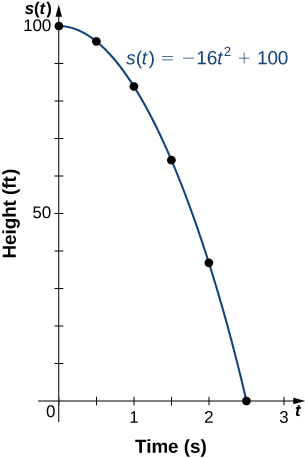
\includegraphics[width=\linewidth]{external/CNX_Calc_Figure_01_01_009.jpg}
\end{image}%
\tcblower
\end{figureptx}%
%
\end{enumerate}
\end{example}
Note that for this function and the function \(f(x)=-4x+2\) graphed in \hyperref[x:figure:CNX_Calc_Figure_01_01_007]{Figure~{\xreffont\ref{x:figure:CNX_Calc_Figure_01_01_007}}}, the values of \(f(x)\) are getting smaller as \(x\) is getting larger. A function with this property is said to be decreasing. On the other hand, for the function \(f(x)=\sqrt{x+3}+1\) graphed in \hyperref[x:figure:CNX_Calc_Figure_01_01_008]{Figure~{\xreffont\ref{x:figure:CNX_Calc_Figure_01_01_008}}}, the values of \(f(x)\) are getting larger as the values of \(x\) are getting larger. A function with this property is said to be increasing. It is important to note, however, that a function can be increasing on some interval or intervals and decreasing over a different interval or intervals. For example, using our temperature function in \hyperref[x:figure:CNX_Calc_Figure_01_01_005]{Figure~{\xreffont\ref{x:figure:CNX_Calc_Figure_01_01_005}}}, we can see that the function is decreasing on the interval \((0,4),\) increasing on the interval \((4,14),\) and then decreasing on the interval \((14,23).\) We make the idea of a function increasing or decreasing over a particular interval more precise in the next definition.%
\begin{definition}{}{g:definition:idm1622443496}%
We say that a function \(f\) is \terminology{increasing on the interval \(I\)} if for all \(x_1,x_2\in I,\)%
%
\begin{equation*}
f(x_1) \leq  f(x_2) \text{ when } x_1 < x_2.
\end{equation*}
We say \(f\) is \terminology{strictly increasing on the interval \(I\)} if for all \(x_1,x_2\in I,\)%
%
\begin{equation*}
f(x_1) < f(x_2) \text{ when } x_1 < x_2.
\end{equation*}
We say that a function \(f\) is \terminology{decreasing on the interval \(I\)} if for all \(x_1,x_2\in I,\)%
%
\begin{equation*}
f(x_1)\geq f(x_2) \text{ when }x_1 < x_2.
\end{equation*}
We say that a function \(f\) is \terminology{strictly decreasing on the interval \(I\)} if for all \(x_1,x_2\in I,\)%
%
\begin{equation*}
f(x_1) > f(x_2) \text{ when }x_1 < x_2.
\end{equation*}
\end{definition}
For example, the function \(f(x)=3x\) is increasing on the interval \((-\infty, \infty)\) because \(3x_1 < 3x_2\) whenever \(x_1 < x_2.\) On the other hand, the function \(f(x)=-x^3\) is decreasing on the interval \((-\infty, \infty)\) because \(-(x_1)^3 > -(x_2)^3\) whenever \(x_1 < x_2\) (\hyperref[x:figure:CNX_Calc_Figure_01_01_010]{Figure~{\xreffont\ref{x:figure:CNX_Calc_Figure_01_01_010}}}).%
\begin{figureptx}{(a) The function \(f(x)=3x\) is increasing on the interval  \((-\infty, \infty)\) (b) The function \(f(x)=-x^3\) is decreasing on the interval  \((-\infty, \infty)\)}{x:figure:CNX_Calc_Figure_01_01_010}{}%
\begin{image}{0}{1}{0}%
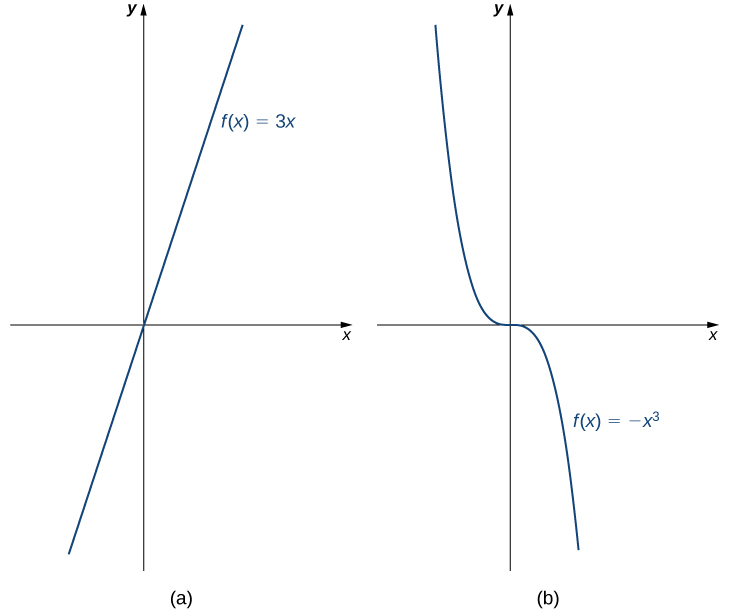
\includegraphics[width=\linewidth]{external/CNX_Calc_Figure_01_01_010.jpg}
\end{image}%
\tcblower
\end{figureptx}%
\begin{definition}{}{g:definition:idm1622431208}%
We say that a function \(f\) is \terminology{concave up on the interval \(I\)} if the graph bends upwards on \(I\).%
\par
We say that a function \(f\) is \terminology{concave down on the interval \(I\)} if the graph bends downwards on \(I\).%
\end{definition}
For example, the function \(f(x)=x^2+1\) is concave up on the entire real line, that is, on the interval \((-\infty,\infty)\) since the graph of \(f\) bends upwards. Notice that a function may not be concave up\slash{}concave down everywhere. It may change concavity. This is illustrated in the following example.%
\par
Observe that \(g(x)=x^3\) is concave down on the interval \((-\infty,0)\) since the graph of \(g\) bends upwards on this interval. Moreover, \(g\) is concave up on the interval \((0,\infty)\) since the graph of \(g\) bends downwards on this interval.%
\end{subsectionptx}
%
%
\typeout{************************************************}
\typeout{Subsection 1.1.3 Combining Functions}
\typeout{************************************************}
%
\begin{subsectionptx}{Combining Functions}{}{Combining Functions}{}{}{g:subsection:idm1622420840}
\begin{introduction}{}%
Now that we have reviewed the basic characteristics of functions, we can see what happens to these properties when we combine functions in different ways, using basic mathematical operations to create new functions. For example, if the cost for a company to manufacture \(x\) items is described by the function \(C(x)\) and the revenue created by the sale of \(x\) items is described by the function \(R(x),\) then the profit on the manufacture and sale of \(x\) items is defined as \(P(x)=R(x)-C(x).\) Using the difference between two functions, we created a new function.%
\par
Alternatively, we can create a new function by composing two functions. For example, given the functions \(f(x)=x^2\) and \(g(x)=3x+1,\) the composite function \(f\circ g\) is defined such that%
%
\begin{equation*}
(f\circ g)(x)=f(g(x))=(g(x))^2=(3x+1)^2.
\end{equation*}
The composite function \(g\circ f\) is defined such that%
%
\begin{equation*}
(g\circ f)(x)=g(f(x))=3f(x)+1=3x^2+1.
\end{equation*}
Note that these two new functions are different from each other.%
\end{introduction}%
%
%
\typeout{************************************************}
\typeout{Subsubsection 1.1.3.1 Combining Functions with Mathematical Operators}
\typeout{************************************************}
%
\begin{subsubsectionptx}{Combining Functions with Mathematical Operators}{}{Combining Functions with Mathematical Operators}{}{}{g:subsubsection:idm1622414184}
To combine functions using mathematical operators, we simply write the functions with the operator and simplify. Given two functions \(f\) and \(g,\) we can define four new functions:%
%
\begin{align*}
(f+g)(x)=f(x)+g(x) \amp \amp \text{Sum} \\
(f-g)(x)=f(x)-g(x) \amp \amp \text{Difference} \\
(f·g)(x)=f(x)g(x) \amp \amp \text{Product} \\
\left(\frac{f}{g}\right)(x)=\frac{f(x)}{g(x)} \text{ for } g(x) \neq 0 \amp \amp \text{Quotient} 
\end{align*}
\begin{example}{Combining Functions Using Mathematical Operations.}{g:example:idm1622408680}%
Given the functions \(f(x)=2x-3\) and \(g(x)=x^2-1,\) find each of the following functions and state its domain.%
%
\begin{enumerate}
\item{}\(\displaystyle (f+g)(x)\)%
\item{}\(\displaystyle (f-g)(x)\)%
\item{}\(\displaystyle (f·g)(x)\)%
\item{}\(\displaystyle (\frac{f}{g})(x)\)%
\end{enumerate}
\par\smallskip%
\noindent\textbf{\blocktitlefont Solution}.\hypertarget{g:solution:idm1622404200}{}\quad{}%
\begin{enumerate}
\item{}\((f+g)(x)=(2x-3)+(x^2-1)=x^2+2x-4.\) The domain of this function is the interval \((-\infty,\infty).\)%
\item{}\((f-g)(x)=(2x-3)-(x^2-1)=-x^2+2x-2.\) The domain of this function is the interval \((-\infty,\infty).\)%
\item{}\((f·g)(x)=(2x-3)(x^2-1)=2x^3-3x^2-2x+3.\) The domain of this function is the interval \((-\infty,\infty).\)%
\item{}\(\left(\frac{f}{g}\right)(x)=\frac{2x-3}{x^2-1}.\) The domain of this function is \(\{x|x\neq\pm 1\}.\)%
\end{enumerate}
\end{example}
\begin{inlineexercise}{}{g:exercise:idm1622405864}%
For \(f(x)=x^2+3\) and \(g(x)=2x-5,\) find \((f/g)(x)\) and state its domain.%
\par\smallskip%
\noindent\textbf{\blocktitlefont Hint}.\hypertarget{g:hint:idm1622403304}{}\quad{}The new function \((f/g)(x)\) is a quotient of two functions. For what values of \(x\) is the denominator zero?%
\par\smallskip%
\noindent\textbf{\blocktitlefont Solution}.\hypertarget{g:solution:idm1622400872}{}\quad{}\((\frac{f}{g})(x)=\frac{x^2+3}{2x-5}.\) The domain is \(\{x|x\neq\frac{5}{2}\}.\)%
\end{inlineexercise}%
\end{subsubsectionptx}
%
%
\typeout{************************************************}
\typeout{Subsubsection 1.1.3.2 Function Composition}
\typeout{************************************************}
%
\begin{subsubsectionptx}{Function Composition}{}{Function Composition}{}{}{g:subsubsection:idm1622396776}
When we compose functions, we take a function of a function. For example, suppose the temperature \(T\) on a given day is described as a function of time \(t\) (measured in hours after midnight) as in \hyperref[x:table:fs-id1170572114646]{Table~{\xreffont\ref{x:table:fs-id1170572114646}}}. Suppose the cost \(C,\) to heat or cool a building for 1 hour, can be described as a function of the temperature \(T.\) Combining these two functions, we can describe the cost of heating or cooling a building as a function of time by evaluating \(C(T(t)).\) We have defined a new function, denoted \(C\circ T,\) which is defined such that \((C\circ T)(t)=C(T(t))\) for all \(t\) in the domain of \(T.\) This new function is called a composite function. We note that since cost is a function of temperature and temperature is a function of time, it makes sense to define this new function \((C\circ T)(t).\) It does not make sense to consider \((T\circ C)(t),\) because temperature is not a function of cost.%
\begin{definition}{}{g:definition:idm1622394600}%
Consider the function \(f\) with domain \(A\) and range \(B,\) and the function \(g\) with domain \(D\) and range \(E.\) If \(B\) is a subset of \(D,\) then the \terminology{composite function} \((g\circ  f)(x)\) is the function with domain \(A\) such that%
%
\begin{equation*}
(g\circ f)(x)=g(f(x)).
\end{equation*}
\end{definition}
A composite function \(g\circ f\) can be viewed in two steps. First, the function \(f\) maps each input \(x\) in the domain of \(f\) to its output \(f(x)\) in the range of \(f.\) Second, since the range of \(f\) is a subset of the domain of \(g,\) the output \(f(x)\) is an element in the domain of \(g,\) and therefore it is mapped to an output \(g(f(x))\) in the range of \(g.\) In \hyperref[x:figure:CNX_Calc_Figure_01_01_011]{Figure~{\xreffont\ref{x:figure:CNX_Calc_Figure_01_01_011}}}, we see a visual image of a composite function.%
\begin{figureptx}{For the composite function \(g\circ f,\) we have \((g\circ f)(1)=4,(g\circ f)(2)=5,\) and \((g\circ f)(3)=4.\)}{x:figure:CNX_Calc_Figure_01_01_011}{}%
\begin{image}{0.25}{0.5}{0.25}%
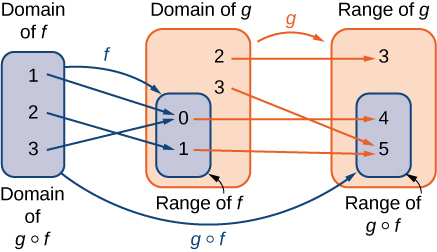
\includegraphics[width=\linewidth]{external/CNX_Calc_Figure_01_01_011.jpg}
\end{image}%
\tcblower
\end{figureptx}%
\begin{example}{Compositions of Functions Defined by Formulas.}{x:example:fs-id1170572481349}%
Consider the functions \(f(x)=x^2+1\) and \(g(x)=1/x.\)%
%
\begin{enumerate}
\item{}Find \((g\circ f)(x)\) and state its domain and range.%
\item{}Evaluate \((g\circ f)(4),(g\circ f)(-1/2).\)%
\item{}Find \((f\circ g)(x)\) and state its domain and range.%
\item{}Evaluate \((f\circ g)(4),(f\circ g)(-1/2).\)%
\end{enumerate}
\par\smallskip%
\noindent\textbf{\blocktitlefont Solution}.\hypertarget{x:solution:fs-id1170572222941}{}\quad{}%
\begin{enumerate}
\item{}We can find the formula for \((g\circ f)(x)\) in two different ways. We could write%
\begin{equation*}
(g\circ f)(x)=g(f(x))=g(x^2+1)=\frac{1}{x^2+1}.
\end{equation*}
Alternatively, we could write%
\begin{equation*}
(g\circ f)(x)=g(f(x))=\frac{1}{f(x)}=\frac{1}{x^2+1}.
\end{equation*}
Since \(x^2+1\neq 0\) for all real numbers \(x,\) the domain of \((g\circ f)(x)\) is the set of all real numbers. Since \(0 \lt 1/(x^2+1) \leq  1,\) the range is, at most, the interval \((0,1].\) To show that the range is this entire interval, we let \(y=1/(x^2+1)\) and solve this equation for \(x\) to show that for all \(y\) in the interval \((0,1],\) there exists a real number \(x\) such that \(y=1/(x^2+1).\) Solving this equation for \(x,\) we see that \(x^2+1=1/y,\) which implies that%
\begin{equation*}
x=\pm\sqrt{\frac{1}{y}-1}.
\end{equation*}
If \(y\) is in the interval \((0,1],\) the expression under the radical is nonnegative, and therefore there exists a real number \(x\) such that \(1/(x^2+1)=y.\) We conclude that the range of \(g\circ f\) is the interval \((0,1].\)%
\item{}\((g\circ f)(4)=g(f(4))=g(4^2+1)=g(17)=\frac{1}{17}\)  and \((g\circ f)(-\frac{1}{2})=g(f(-\frac{1}{2}))=g((-\frac{1}{2})^2+1)=g(\frac{5}{4})=\frac{4}{5}\)%
\item{}We can find a formula for \((f\circ g)(x)\) in two ways. First, we could write%
\begin{equation*}
(f\circ g)(x)=f(g(x))=f\left(\frac{1}{x}\right)=\left(\frac{1}{x}\right)^2+1.
\end{equation*}
Alternatively, we could write%
\begin{equation*}
(f\circ g)(x)=f(g(x))=(g(x))^2+1=\left(\frac{1}{x}\right)^2+1.
\end{equation*}
The domain of \(f\circ g\) is the set of all real numbers \(x\) such that \(x\neq 0.\) To find the range of \(f,\) we need to find all values \(y\) for which there exists a real number \(x\neq0\) such that%
\begin{equation*}
\left(\frac{1}{x}\right)^2+1=y.
\end{equation*}
Solving this equation for \(x,\) we see that we need \(x\) to satisfy%
\begin{equation*}
\left(\frac{1}{x}\right)^2=y-1,
\end{equation*}
which simplifies to%
\begin{equation*}
\frac{1}{x}=\pm\sqrt{y-1}.
\end{equation*}
Finally, we obtain%
\begin{equation*}
x=\pm\frac{1}{\sqrt{y-1}}.
\end{equation*}
Since \(1/\sqrt{y-1}\) is a real number if and only if \(y\gt 1,\) the range of \(f\) is the set \(\{y|y\gt 1\}.\)%
\item{}\((f\circ g)(4)=f(g(4))=f(\frac{1}{4})=(\frac{1}{4})^2+1=\frac{17}{16}\) \((f\circ g)(-\frac{1}{2})=f(g(-\frac{1}{2}))=f(-2)=(-2)^2+1=5\)%
\end{enumerate}
\end{example}
In \hyperref[x:example:fs-id1170572481349]{Example~{\xreffont\ref{x:example:fs-id1170572481349}}}, we can see that \((f\circ g)(x)\neq(g\circ f)(x).\) This tells us, in general terms, that the order in which we compose functions matters.%
\begin{inlineexercise}{}{g:exercise:idm1622358120}%
Let \(f(x)=2-5x.\) Let \(g(x)=\sqrt{x}.\) Find \((f\circ g)(x).\)%
\par\smallskip%
\noindent\textbf{\blocktitlefont Solution}.\hypertarget{g:solution:idm1622351208}{}\quad{}\((f\circ g)(x)=2-5\sqrt{x}.\)%
\end{inlineexercise}%
\begin{example}{Composition of Functions Defined by Tables.}{g:example:idm1622352360}%
Test%
\par
Consider the functions \(f\) and \(g\) described by \hyperref[x:table:fs-id1170572173822]{Table~{\xreffont\ref{x:table:fs-id1170572173822}}} and \hyperref[x:table:fs-id1170572550754]{Table~{\xreffont\ref{x:table:fs-id1170572550754}}}.%
\begin{tableptx}{\textbf{}}{x:table:fs-id1170572173822}{}%
\centering%
{\tabularfont%
\begin{tabular}{lllllllll}
\multicolumn{1}{c}{\(x\)}&\multicolumn{1}{c}{\(-3\)}&\multicolumn{1}{c}{\(-2\)}&\multicolumn{1}{c}{\(-1\)}&\multicolumn{1}{c}{\(0\)}&\multicolumn{1}{c}{\(1\)}&\multicolumn{1}{c}{\(2\)}&\multicolumn{1}{c}{\(3\)}&\multicolumn{1}{c}{\(4\)}\tabularnewline[0pt]
\multicolumn{1}{c}{\(f(x)\)}&\multicolumn{1}{c}{\(0\)}&\multicolumn{1}{c}{\(4\)}&\multicolumn{1}{c}{\(2\)}&\multicolumn{1}{c}{\(4\)}&\multicolumn{1}{c}{\(-2\)}&\multicolumn{1}{c}{\(0\)}&\multicolumn{1}{c}{\(-2\)}&\multicolumn{1}{c}{\(4\)}
\end{tabular}
}%
\end{tableptx}%
\begin{tableptx}{\textbf{}}{x:table:fs-id1170572550754}{}%
\centering%
{\tabularfont%
\begin{tabular}{llllll}
\multicolumn{1}{c}{\(x\)}&\multicolumn{1}{c}{\(-4\)}&\multicolumn{1}{c}{\(-2\)}&\multicolumn{1}{c}{\(0\)}&\multicolumn{1}{c}{\(2\)}&\multicolumn{1}{c}{\(4\)}\tabularnewline[0pt]
\multicolumn{1}{c}{\(g(x)\)}&\multicolumn{1}{c}{\(1\)}&\multicolumn{1}{c}{\(0\)}&\multicolumn{1}{c}{\(3\)}&\multicolumn{1}{c}{\(0\)}&\multicolumn{1}{c}{\(5\)}
\end{tabular}
}%
\end{tableptx}%
%
\begin{enumerate}
\item{}Evaluate \((g\circ f)(3),(g\circ f)(0).\)%
\item{}State the domain and range of \((g\circ f)(x).\)%
\item{}Evaluate \((f\circ f)(3),(f\circ f)(1).\)%
\item{}State the domain and range of \((f\circ f)(x).\)%
\end{enumerate}
\par\smallskip%
\noindent\textbf{\blocktitlefont Solution}.\hypertarget{g:solution:idm1622254440}{}\quad{}%
\begin{enumerate}
\item{}\((g\circ f)(3)=g(f(3))=g(-2)=0\) \((g\circ f)(0)=g(4)=5\)%
\item{}The domain of \(g\circ f\) is the set \(\{-3,-2,-1,0,1,2,3,4\}.\) Since the range of \(f\) is the set \(\{-2,0,2,4\},\) the range of \(g\circ f\) is the set \({0,3,5}.\)%
\item{}\((f\circ f)(3)=f(f(3))=f(-2)=4\) \((f\circ f)(1)=f(f(1))=f(-2)=4\)%
\item{}The domain of \(f\circ f\) is the set \(\{-3,-2,-1,0,1,2,3,4\}.\) Since the range of \(f\) is the set \(\{-2,0,2,4\},\) the range of \(f\circ f\) is the set \(\{0,4\}.\)%
\end{enumerate}
\end{example}
\begin{example}{Application Involving a Composite Function.}{g:example:idm1622247400}%
A store is advertising a sale of \(20\%\) off all merchandise. Caroline has a coupon that entitles her to an additional \(15\%\) off any item, including sale merchandise. If Caroline decides to purchase an item with an original price of \(x\) dollars, how much will she end up paying if she applies her coupon to the sale price? Solve this problem by using a composite function.%
\par\smallskip%
\noindent\textbf{\blocktitlefont Solution}.\hypertarget{g:solution:idm1622247016}{}\quad{}Since the sale price is \(20\%\) off the original price, if an item is \(x\) dollars, its sale price is given by \(f(x)=0.80x.\) Since the coupon entitles an individual to \(15\%\) off the price of any item, if an item is \(y\) dollars, the price, after applying the coupon, is given by \(g(y)=0.85y.\) Therefore, if the price is originally \(x\) dollars, its sale price will be \(f(x)=0.80x\) and then its final price after the coupon will be \(g(f(x))=0.85(0.80x)=0.68x.\)%
\end{example}
\begin{inlineexercise}{}{g:exercise:idm1622242792}%
If items are on sale for \(10\%\) off their original price, and a customer has a coupon for an additional \(30\%\) off, what will be the final price for an item that is originally \(x\) dollars, after applying the coupon to the sale price?%
\par\smallskip%
\noindent\textbf{\blocktitlefont Hint}.\hypertarget{g:hint:idm1622237544}{}\quad{}The sale price of an item with an original price of \(x\) dollars is \(f(x)=0.90x.\) The coupon price for an item that is \(y\) dollars is \(g(y)=0.70y.\)%
\par\smallskip%
\noindent\textbf{\blocktitlefont Solution}.\hypertarget{g:solution:idm1622238824}{}\quad{}\((g\circ f)(x)=0.63x\)%
\end{inlineexercise}%
\end{subsubsectionptx}
\end{subsectionptx}
%
%
\typeout{************************************************}
\typeout{Subsection 1.1.4 Symmetry of Functions}
\typeout{************************************************}
%
\begin{subsectionptx}{Symmetry of Functions}{}{Symmetry of Functions}{}{}{g:subsection:idm1622237416}
The graphs of certain functions have symmetry properties that help us understand the function and the shape of its graph. For example, consider the function \(f(x)=x^4-2x^2-3\) shown in \hyperref[x:figure:CNX_Calc_Figure_01_01_012]{Figure~{\xreffont\ref{x:figure:CNX_Calc_Figure_01_01_012}}}(a). If we take the part of the curve that lies to the right of the \(y\)-axis and flip it over the \(y\)-axis, it lays exactly on top of the curve to the left of the \(y\)-axis. In this case, we say the function has \terminology{symmetry about the \(y\)-axis}. On the other hand, consider the function \(f(x)=x^3-4x\) shown in \hyperref[x:figure:CNX_Calc_Figure_01_01_012]{Figure~{\xreffont\ref{x:figure:CNX_Calc_Figure_01_01_012}}}(b). If we take the graph and rotate it \(180^{\circ}\) about the origin, the new graph will look exactly the same. In this case, we say the function has \terminology{symmetry about the origin}.%
\begin{figureptx}{(a) A graph that is symmetric about the \(y\)-axis. (b) A graph that is symmetric about the origin.}{x:figure:CNX_Calc_Figure_01_01_012}{}%
\begin{image}{0}{1}{0}%
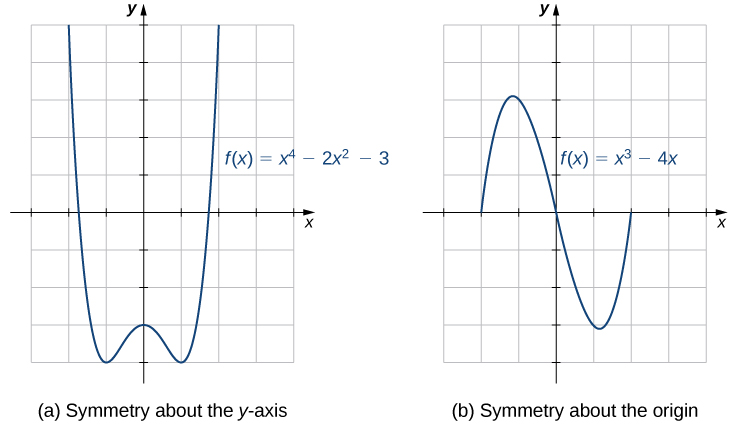
\includegraphics[width=\linewidth]{external/CNX_Calc_Figure_01_01_012.jpg}
\end{image}%
\tcblower
\end{figureptx}%
If we are given the graph of a function, it is easy to see whether the graph has one of these symmetry properties. But without a graph, how can we determine algebraically whether a function \(f\) has symmetry? Looking at \hyperref[x:figure:CNX_Calc_Figure_01_01_012]{Figure~{\xreffont\ref{x:figure:CNX_Calc_Figure_01_01_012}}}(a) again, we see that since \(f\) is symmetric about the \(y\)-axis, if the point \((x,y)\) is on the graph, the point \((-x,y)\) is on the graph. In other words, \(f(-x)=f(x).\) If a function \(f\) has this property, we say \(f\) is an even function, which has symmetry about the \(y\)-axis. For example, \(f(x)=x^2\) is even because%
%
\begin{equation*}
f(-x)=(-x)^2=x^2=f(x).
\end{equation*}
In contrast, looking at \hyperref[x:figure:CNX_Calc_Figure_01_01_012]{Figure~{\xreffont\ref{x:figure:CNX_Calc_Figure_01_01_012}}}(b) again, if a function \(f\) is symmetric about the origin, then whenever the point \((x,y)\) is on the graph, the point \((-x,-y)\) is also on the graph. In other words, \(f(-x)=-f(x).\) If \(f\) has this property, we say \(f\) is an odd function, which has symmetry about the origin. For example, \(f(x)=x^3\) is odd because%
%
\begin{equation*}
f(-x)=(-x)^3=-x^3=-f(x).
\end{equation*}
\begin{definition}{}{g:definition:idm1622222952}%
If \(f(x)=f(-x)\) for all \(x\) in the domain of \(f,\) then \(f\) is an \terminology{even function}. An even function is symmetric about the \(y\)-axis.%
\par
If \(f(-x)=-f(x)\) for all \(x\) in the domain of \(f,\) then \(f\) is an \terminology{odd function}. An odd function is symmetric about the origin.%
\end{definition}
\begin{example}{Even and Odd Functions.}{g:example:idm1622211304}%
Determine whether each of the following functions is even, odd, or neither.%
%
\begin{enumerate}
\item{}\(\displaystyle f(x)=-5x^4+7x^2-2\)%
\item{}\(\displaystyle f(x)=2x^5-4x+5\)%
\item{}\(\displaystyle f(x)=\frac{3x}{x^2+1}\)%
\end{enumerate}
\par\smallskip%
\noindent\textbf{\blocktitlefont Solution}.\hypertarget{g:solution:idm1622211560}{}\quad{}To determine whether a function is even or odd, we evaluate \(f(-x)\) and compare it to \(f(x)\) and \(-f(x).\)%
%
\begin{enumerate}
\item{}\(f(-x)=-5(-x)^4+7(-x)^2-2=-5x^4+7x^2-2=f(x).\) Therefore, \(f\) is even.%
\item{}\(f(-x)=2(-x)^5-4(-x)+5=-2x^5+4x+5.\) Now, \(f(-x)\neq f(x).\) Furthermore, noting that \(-f(x)=-2x^5+4x-5,\) we see that \(f(-x)\neq-f(x).\) Therefore, \(f\) is neither even nor odd.%
\item{}\(f(-x)=3(-x)/((-x)^2+1=-3x/(x^2+1)=-[3x/(x^2+1)]=-f(x).\) Therefore, \(f\) is odd.%
\end{enumerate}
\end{example}
\begin{inlineexercise}{}{g:exercise:idm1622206696}%
Determine whether \(f(x)=4x^3-5x\) is even, odd, or neither.%
\par\smallskip%
\noindent\textbf{\blocktitlefont Hint}.\hypertarget{g:hint:idm1622206056}{}\quad{}Compare \(f(-x)\) with \(f(x)\) and \(-f(x).\)%
\par\smallskip%
\noindent\textbf{\blocktitlefont Solution}.\hypertarget{g:solution:idm1622204264}{}\quad{}\(f(x)\) is odd.%
\end{inlineexercise}%
One symmetric function that arises frequently is the \terminology{absolute value function}, written as \(|x|.\) The absolute value function is defined as%
%
\begin{equation*}
f(x)=\begin{cases}x \amp x \lt 0 \\ x \amp x \geq 0\end{cases}\text{.}
\end{equation*}
Some students describe this function by stating that it “makes everything positive.” By the definition of the absolute value function, we see that if \(x \lt 0,\) then \(|x|=-x \gt 0,\) and if \(x\gt 0,\) then \(|x|=x\gt 0.\) However, for \(x=0,|x|=0.\) Therefore, it is more accurate to say that for all nonzero inputs, the output is positive, but if \(x=0,\) the output \(|x|=0.\) We conclude that the range of the absolute value function is \(\{y|y \geq 0\}.\) In \hyperref[x:figure:CNX_Calc_Figure_01_01_013]{Figure~{\xreffont\ref{x:figure:CNX_Calc_Figure_01_01_013}}}, we see that the absolute value function is symmetric about the \(y\)-axis and is therefore an even function.%
\begin{figureptx}{The graph of \(f(x)=|x|\) is symmetric about the \(y\)-axis.}{x:figure:CNX_Calc_Figure_01_01_013}{}%
\begin{image}{0.25}{0.5}{0.25}%
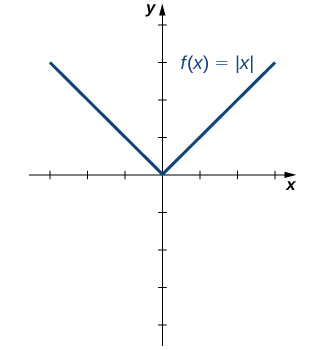
\includegraphics[width=\linewidth]{external/CNX_Calc_Figure_01_01_013.jpg}
\end{image}%
\tcblower
\end{figureptx}%
\begin{example}{Working with the Absolute Value Function.}{g:example:idm1622194664}%
Find the domain and range of the function \(f(x)=2|x-3|+4.\)%
\par\smallskip%
\noindent\textbf{\blocktitlefont Solution}.\hypertarget{g:solution:idm1622193768}{}\quad{}Since the absolute value function is defined for all real numbers, the domain of this function is \((-\infty,\infty).\) Since \(|x-3|\geq 0\) for all \(x,\) the function \(f(x)=2|x-3|+4\geq 4.\) Therefore, the range is, at most, the set \(\{y|y\geq 4\}.\) To see that the range is, in fact, this whole set, we need to show that for \(y\geq 4\) there exists a real number \(x\) such that%
%
\begin{equation*}
2|x-3|+4=y.
\end{equation*}
A real number \(x\) satisfies this equation as long as%
%
\begin{equation*}
|x-3|=\frac{1}{2}(y-4).
\end{equation*}
Since \(y\geq 4,\) we know \(y-4\geq 0,\) and thus the right-hand side of the equation is nonnegative, so it is possible that there is a solution. Furthermore,%
%
\begin{equation*}
|x-3|=\begin{cases}-(x-3) \amp \text{ if } x\lt  3 \\x-3 \amp \text{ if }x \geq 3. \end{cases}
\end{equation*}
Therefore, we see there are two solutions:%
%
\begin{equation*}
x=\pm\frac{1}{2}(y-4)+3.
\end{equation*}
The range of this function is \(\{y|y\geq 4\}.\)%
\end{example}
\begin{inlineexercise}{}{g:exercise:idm1622183784}%
For the function \(f(x)=|x+2|-4,\) find the domain and range.%
\par\smallskip%
\noindent\textbf{\blocktitlefont Hint}.\hypertarget{g:hint:idm1622185832}{}\quad{}\(|x+2|\geq 0\) for all real numbers \(x.\)%
\par\smallskip%
\noindent\textbf{\blocktitlefont Solution}.\hypertarget{g:solution:idm1622182760}{}\quad{}Domain = \((-\infty,\infty),\) range = \(\{y|y\geq -4\}.\)%
\end{inlineexercise}%
\end{subsectionptx}
%
%
\typeout{************************************************}
\typeout{Subsection 1.1.5 Key Concepts}
\typeout{************************************************}
%
\begin{subsectionptx}{Key Concepts}{}{Key Concepts}{}{}{g:subsection:idm1622179944}
%
\begin{enumerate}
\item{}A function is a mapping from a set of inputs to a set of outputs with exactly one output for each input.%
\item{}If no domain is stated for a function \(y=f(x),\) the domain is considered to be the set of all real numbers \(x\) for which the function is defined.%
\item{}When sketching the graph of a function \(f,\) each vertical line may intersect the graph, at most, once.%
\item{}A function may have any number of zeros, but it has, at most, one \(y\)-intercept.%
\item{}To define the composition \(g\circ f,\) the range of \(f\) must be contained in the domain of \(g.\)%
\item{}Even functions are symmetric about the \(y\)-axis whereas odd functions are symmetric about the origin.%
\end{enumerate}
\end{subsectionptx}
%
%
\typeout{************************************************}
\typeout{Subsection 1.1.6 Key Equations}
\typeout{************************************************}
%
\begin{subsectionptx}{Key Equations}{}{Key Equations}{}{}{g:subsection:idm1622176616}
%
\begin{enumerate}
\item{}Composition of two functions \((g\circ f)(x)=g(f(x))\)%
\item{}Absolute value function%
\begin{equation*}
f(x)=\begin{cases}x \amp x \lt 0 \\ x \amp x \geq 0\end{cases}\text{.}
\end{equation*}
%
\end{enumerate}
\end{subsectionptx}
This book is a custom edition based on OpenStax Calculus Volume 1. You can download the original for free at https:\slash{}\slash{}openstax.org\slash{}details\slash{}books\slash{}calculus-volume-1.%
\end{sectionptx}
%
%
\typeout{************************************************}
\typeout{Section 1.2 Basic Classes of Functions}
\typeout{************************************************}
%
\begin{sectionptx}{Basic Classes of Functions}{}{Basic Classes of Functions}{}{}{x:section:sec_Ch1Sec2}
\begin{introduction}{Learning Objectives.}%
%
\begin{itemize}[label=\textbullet]
\item{}Calculate the slope of a linear function and interpret its meaning.%
\item{}Recognize the degree of a polynomial.%
\item{}Find the roots of a quadratic polynomial.%
\item{}Describe the graphs of basic odd and even polynomial functions.%
\item{}Identify a rational function.%
\item{}Describe the graphs of power and root functions.%
\item{}Explain the difference between algebraic and transcendental functions.%
\item{}Graph a piecewise-defined function.%
\item{}Sketch the graph of a function that has been shifted, stretched, or reflected from its initial graph position.%
\end{itemize}
We have studied the general characteristics of functions, so now let's examine some specific classes of functions. We begin by reviewing the basic properties of linear and quadratic functions, and then generalize to include higher-degree polynomials. By combining root functions with polynomials, we can define general algebraic functions and distinguish them from the transcendental functions we examine later in this chapter. We finish the section with examples of piecewise-defined functions and take a look at how to sketch the graph of a function that has been shifted, stretched, or reflected from its initial form.%
\end{introduction}%
%
%
\typeout{************************************************}
\typeout{Subsection 1.2.1 Linear Functions and Slope}
\typeout{************************************************}
%
\begin{subsectionptx}{Linear Functions and Slope}{}{Linear Functions and Slope}{}{}{g:subsection:idm1622166120}
The easiest type of function to consider is a \terminology{linear function}. Linear functions have the form \(f(x)=ax+b,\) where \(a\) and \(b\) are constants. In \hyperref[x:figure:CNX_Calc_Figure_01_02_001]{Figure~{\xreffont\ref{x:figure:CNX_Calc_Figure_01_02_001}}}, we see examples of linear functions when \(a\) is positive, negative, and zero. Note that if \(a\gt  0 ,\) the graph of the line rises as \(x\) increases. In other words, \(f(x)=ax+b\) is increasing on \((-\infty,\infty).\) If \(a\lt  0 ,\) the graph of the line falls as \(x\) increases. In this case, \(f(x)=ax+b\) is decreasing on \((-\infty,\infty).\) If \(a= 0 ,\) the line is horizontal.%
\begin{figureptx}{These linear functions are increasing or decreasing on \((-\infty, \infty)\) and one function is a horizontal line.}{x:figure:CNX_Calc_Figure_01_02_001}{}%
\begin{image}{0.25}{0.5}{0.25}%
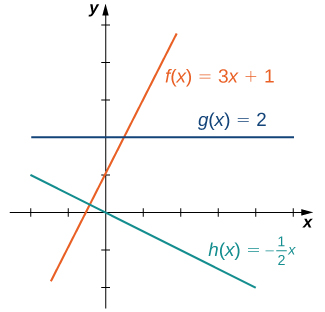
\includegraphics[width=\linewidth]{external/CNX_Calc_Figure_01_02_001.jpg}
\end{image}%
\tcblower
\end{figureptx}%
As suggested by \hyperref[x:figure:CNX_Calc_Figure_01_02_001]{Figure~{\xreffont\ref{x:figure:CNX_Calc_Figure_01_02_001}}}, the graph of any linear function is a line. One of the distinguishing features of a line is its slope. The \terminology{slope} is the change in \(y\) for each unit change in \(x.\) The slope measures both the steepness and the direction of a line. If the slope is positive, the line points upward when moving from left to right. If the slope is negative, the line points downward when moving from left to right. If the slope is zero, the line is horizontal. To calculate the slope of a line, we need to determine the ratio of the change in \(y\) versus the change in \(x.\) To do so, we choose any two points \((x_1,y_1)\) and \((x_2,y_2)\) on the line and calculate \(\frac{y_2-y_1}{x_2-x_1}.\) In \hyperref[x:figure:CNX_Calc_Figure_01_02_002]{Figure~{\xreffont\ref{x:figure:CNX_Calc_Figure_01_02_002}}}, we see this ratio is independent of the points chosen.%
\begin{figureptx}{For any linear function, the slope \((y_2-y_1) /(x_2-x_1)\) is independent of the choice of points \((x_1,y_1)\) and \((x_2,y_2)\) on the line.}{x:figure:CNX_Calc_Figure_01_02_002}{}%
\begin{image}{0.25}{0.5}{0.25}%
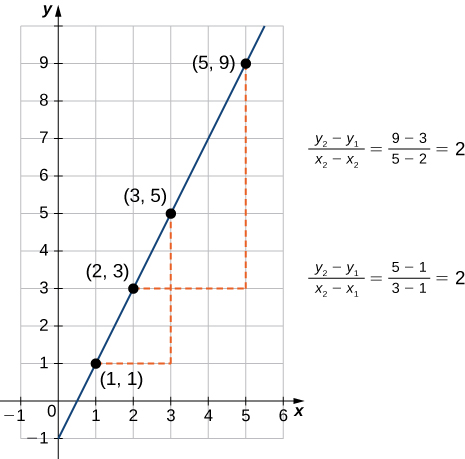
\includegraphics[width=\linewidth]{external/CNX_Calc_Figure_01_02_021.jpg}
\end{image}%
\tcblower
\end{figureptx}%
\begin{definition}{}{g:definition:idm1622150888}%
Consider line \(L\) passing through points \((x_1,y_1)\) and \((x_2,y_2).\) Let \(\Delta y=y_2-y_1\) and \(\Delta x=x_2-x_1\) denote the changes in \(y\) and \(x,\) respectively. The \terminology{slope} of the line is%
%
\begin{equation*}
m= \frac{y_2-y_1}{x_2-x_1}= \frac{\Delta y}{\Delta x}.
\end{equation*}
\end{definition}
We now examine the relationship between slope and the formula for a linear function. Consider the linear function given by the formula \(f(x)=ax+b.\) As discussed earlier, we know the graph of a linear function is given by a line. We can use our definition of slope to calculate the slope of this line. As shown, we can determine the slope by calculating \((y_2-y_1) /(x_2-x_1)\) for any points \((x_1,y_1)\) and \((x_2,y_2)\) on the line. Evaluating the function \(f\) at \(x= 0 ,\) we see that \(( 0 ,b)\) is a point on this line. Evaluating this function at \(x= 1 ,\) we see that \(( 1 ,a+b)\) is also a point on this line. Therefore, the slope of this line is%
%
\begin{equation*}
\frac{(a+b)-b}{1 - 0}=a.
\end{equation*}
We have shown that the coefficient \(a\) is the slope of the line. We can conclude that the formula \(f(x)=ax+b\) describes a line with slope \(a.\) Furthermore, because this line intersects the \(y\)-axis at the point \(( 0 ,b),\) we see that the \(y\)-intercept for this linear function is \(( 0 ,b).\) We conclude that the formula \(f(x)=ax+b\) tells us the slope, \(a,\) and the \(y\)-intercept, \(( 0 ,b),\) for this line. Since we often use the symbol \(m \) to denote the slope of a line, we can write%
%
\begin{equation*}
f(x)=mx+b
\end{equation*}
to denote the \terminology{slope-intercept form} of a linear function.%
\par
Sometimes it is convenient to express a linear function in different ways. For example, suppose the graph of a linear function passes through the point \((x_1,y_1)\) and the slope of the line is \(m.\) Since any other point \((x,f(x))\) on the graph of \(f\) must satisfy the equation%
%
\begin{equation*}
m= \frac{f(x)-y_1}{x-x_1},
\end{equation*}
this linear function can be expressed by writing%
%
\begin{equation*}
f(x)-y_1=m(x-x_1).
\end{equation*}
We call this equation the \terminology{point-slope equation} for that linear function.%
\par
Since every nonvertical line is the graph of a linear function, the points on a nonvertical line can be described using the slope-intercept or point-slope equations. However, a vertical line does not represent the graph of a function and cannot be expressed in either of these forms. Instead, a vertical line is described by the equation \(x=k\) for some constant \(k.\) Since neither the slope-intercept form nor the point-slope form allows for vertical lines, we use the notation%
%
\begin{equation*}
ax+by=c,
\end{equation*}
where \(a,b\) are both not zero, to denote the \terminology{standard form of a line}.%
\begin{definition}{}{g:definition:idm1622095464}%
Consider a line passing through the point \((x_1,y_1)\) with slope \(m.\) The equation%
%
\begin{equation*}
y-y_1=m(x-x_1)
\end{equation*}
is the \terminology{point-slope equation} for that line.%
\par
Consider a line with slope \(m\) and \(y\)-intercept \(( 0 ,b).\) The equation%
%
\begin{equation*}
y=mx+b
\end{equation*}
is an equation for that line in \terminology{slope-intercept form}.%
\par
The \terminology{standard form of a line} is given by the equation%
%
\begin{equation*}
ax+by=c,
\end{equation*}
where \(a\) and \(b\) are both not zero. This form is more general because it allows for a vertical line, \(x=k.\)%
\end{definition}
\begin{example}{Finding the Slope and Equations of Lines.}{g:example:idm1622086632}%
Consider the line passing through the points \(( 11 , -4 )\) and \(( -4 , 5 ),\) as shown in \hyperref[x:figure:CNX_Calc_Figure_01_02_003]{Figure~{\xreffont\ref{x:figure:CNX_Calc_Figure_01_02_003}}}.%
\begin{figureptx}{Finding the equation of a linear function with a graph that is a line between two given points.}{x:figure:CNX_Calc_Figure_01_02_003}{}%
\begin{image}{0.25}{0.5}{0.25}%
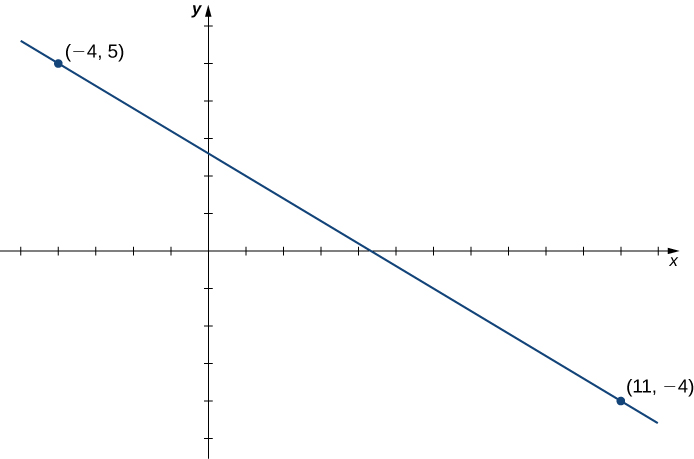
\includegraphics[width=\linewidth]{external/CNX_Calc_Figure_01_02_002.jpg}
\end{image}%
\tcblower
\end{figureptx}%
%
\begin{enumerate}
\item{}Find the slope of the line.%
\item{}Find an equation for this linear function in point-slope form.%
\item{}Find an equation for this linear function in slope-intercept form.%
\end{enumerate}
\par\smallskip%
\noindent\textbf{\blocktitlefont Solution}.\hypertarget{g:solution:idm1622082024}{}\quad{}%
\begin{enumerate}
\item{}The slope of the line is%
\begin{equation*}
m=\frac{y_2-y_1}{x_2-x_1}=\frac{ 5 -( -4 )}{-4 - 11}= \frac{ 9 }{-15 }=- \frac{ 3 }{ 5 }.
\end{equation*}
%
\item{}To find an equation for the linear function in point-slope form, use the slope \(m= -3  / 5 \) and choose any point on the line. If we choose the point \(( 11 , -4 ),\) we get the equation%
\begin{equation*}
f(x)+ 4 =- \frac{ 3 }{ 5 }(x- 11 ).
\end{equation*}
%
\item{}To find an equation for the linear function in slope-intercept form, solve the equation in part b. for \(f(x).\) When we do this, we get the equation%
\begin{equation*}
f(x)=- \frac{ 3}{ 5 }x+ \frac{ 13}{ 5 }.
\end{equation*}
%
\end{enumerate}
\end{example}
\begin{inlineexercise}{}{g:exercise:idm1622078824}%
Consider the line passing through points \(( -3 , 2 )\) and \(( 1 , 4 ).\) Find the slope of the line.%
\par
Find an equation of that line in point-slope form. Find an equation of that line in slope-intercept form.%
\par\smallskip%
\noindent\textbf{\blocktitlefont Hint}.\hypertarget{g:hint:idm1622077288}{}\quad{}The slope \(m=\Delta y /\Delta x.\)%
\par\smallskip%
\noindent\textbf{\blocktitlefont Solution}.\hypertarget{g:solution:idm1622074728}{}\quad{}\(m= 1  / 2 .\) The point-slope form is%
\par
\(y- 4 = \frac{ 1}{ 2 }(x- 1 ).\)%
\par
The slope-intercept form is%
\par
\(y= \frac{ 1}{  2 }x+ \frac{ 7 }{ 2 }.\)%
\end{inlineexercise}%
\begin{example}{A Linear Distance Function.}{g:example:idm1622072168}%
Jessica leaves her house at 5:50 a.m. and goes for a 9-mile run. She returns to her house at 7:08 a.m. Answer the following questions, assuming Jessica runs at a constant pace.%
%
\begin{enumerate}
\item{}Describe the distance \(D\) (in miles) Jessica runs as a linear function of her run time \(t\) (in minutes).%
\item{}Sketch a graph of \(D.\)%
\item{}Interpret the meaning of the slope.%
\end{enumerate}
\par\smallskip%
\noindent\textbf{\blocktitlefont Solution}.\hypertarget{g:solution:idm1622071656}{}\quad{}%
\begin{enumerate}
\item{}At time \(t= 0 ,\) Jessica is at her house, so \(D( 0 )= 0 .\) At time \(t= 78 \) minutes, Jessica has finished running \(9 \) mi, so \(D( 78 )= 9 .\) The slope of the linear function is%
\begin{equation*}
m= \frac{ 9 - 0 }{ 78 - 0 }=\frac{ 3 }{ 26 }.
\end{equation*}
 The \(y\)-intercept is \(( 0 , 0 ),\) so the equation for this linear function is%
\begin{equation*}
D(t)=\frac{ 3 }{ 26 }t.
\end{equation*}
%
\item{}To graph \(D,\) use the fact that the graph passes through the origin and has slope \(m= 3  / 26 .\) \begin{image}{0.25}{0.5}{0.25}%
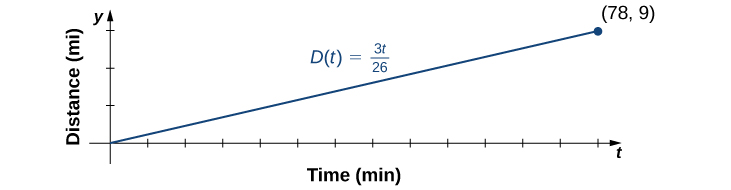
\includegraphics[width=\linewidth]{external/CNX_Calc_Figure_01_02_003.jpg}
\end{image}%
%
\item{}The slope \(m= 3  / 26 \approx 0.115 \) describes the distance (in miles) Jessica runs per minute, or her average velocity.%
\end{enumerate}
\end{example}
\end{subsectionptx}
%
%
\typeout{************************************************}
\typeout{Subsection 1.2.2 Polynomials}
\typeout{************************************************}
%
\begin{subsectionptx}{Polynomials}{}{Polynomials}{}{}{g:subsection:idm1622062184}
\begin{introduction}{}%
A linear function is a special type of a more general class of functions: polynomials. A \terminology{polynomial function} is any function that can be written in the form%
%
\begin{equation*}
f(x)=a_nx^n+a_{n-1}x^{n-1}+\dots+a_1x+a_0
\end{equation*}
for some integer \(n\geq  0 \) and constants \(a_n,a_{n-1}, \dots ,a_0,\) where \(a_n\neq  0 .\) In the case when \(n= 0 ,\) we allow for \(a_0= 0 ;\) if \(a_0= 0 ,\) the function \(f(x)= 0 \) is called the \terminology{zero function}. The value \(n\) is called the \terminology{degree} of the polynomial; the constant \(a_n\) is called the \terminology{leading coefficient}. A linear function of the form \(f(x)=mx+b\) is a polynomial of degree 1 if \(m\neq  0 \) and degree 0 if \(m= 0 .\) A polynomial of degree 0 is also called a \terminology{constant function}. A polynomial function of degree 2 is called a \terminology{quadratic function}. In particular, a quadratic function has the form \(f(x)=ax^2 +bx+c,\) where \(a\neq  0 .\) A polynomial function of degree \(3 \) is called a \terminology{cubic function}.%
\end{introduction}%
%
%
\typeout{************************************************}
\typeout{Subsubsection 1.2.2.1 Power Functions}
\typeout{************************************************}
%
\begin{subsubsectionptx}{Power Functions}{}{Power Functions}{}{}{g:subsubsection:idm1622054632}
Some polynomial functions are power functions. A \terminology{power function} is any function of the form \(f(x)=ax^b ,\) where \(a\) and \(b\) are any real numbers. The exponent in a power function can be any real number, but here we consider the case when the exponent is a positive integer. (We consider other cases later.) If the exponent is a positive integer, then \(f(x)=ax^n\) is a polynomial. If \(n\) is even, then \(f(x)=ax^n\) is an even function because \(f(-x)=a(-x)^n=ax^n\) if \(n\) is even. If \(n\) is odd, then \(f(x)=ax^n\) is an odd function because \(f(-x)=a(-x)^n=-ax^n\) if \(n\) is odd (\hyperref[x:figure:CNX_Calc_Figure_01_02_004]{Figure~{\xreffont\ref{x:figure:CNX_Calc_Figure_01_02_004}}}).%
\begin{figureptx}{(a) For any even integer \(n,f(x)=ax^n\) is an even function. (b) For any odd integer \(n,f(x)=ax^n\) is an odd function.}{x:figure:CNX_Calc_Figure_01_02_004}{}%
\begin{image}{0.25}{0.5}{0.25}%
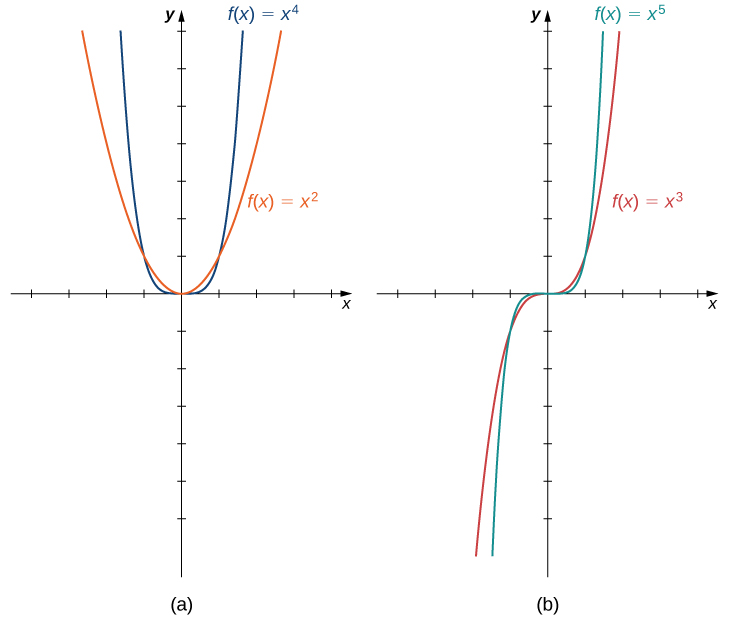
\includegraphics[width=\linewidth]{external/CNX_Calc_Figure_01_02_004.jpg}
\end{image}%
\tcblower
\end{figureptx}%
\end{subsubsectionptx}
%
%
\typeout{************************************************}
\typeout{Subsubsection 1.2.2.2 Behavior at Infinity}
\typeout{************************************************}
%
\begin{subsubsectionptx}{Behavior at Infinity}{}{Behavior at Infinity}{}{}{g:subsubsection:idm1622043368}
To determine the behavior of a function \(f\) as the inputs approach infinity, we look at the values \(f(x)\) as the inputs, \(x,\) become larger. For some functions, the values of \(f(x)\) approach a finite number. For example, for the function \(f(x)= 2 + 1  /x,\) the values \(1  /x\) become closer and closer to zero for all values of \(x\) as they get larger and larger. For this function, we say \(``f(x)\) approaches two as \(x\) goes to infinity,” and we write \(f(x)\to  2 \) as \(x\to \infty.\) The line \(y= 2 \) is a horizontal asymptote for the function \(f(x)= 2 + 1  /x\) because the graph of the function gets closer to the line as \(x\) gets larger.%
\par
For other functions, the values \(f(x)\) may not approach a finite number but instead may become larger for all values of \(x\) as they get larger. In that case, we say \(``f(x)\) approaches infinity as \(x\) approaches infinity,” and we write \(f(x)\to \infty\) as \(x\to \infty.\) For example, for the function \(f(x)= 3 x^2 ,\) the outputs \(f(x)\) become larger as the inputs \(x\) get larger. We can conclude that the function \(f(x)= 3 x^2 \) approaches infinity as \(x\) approaches infinity, and we write \(3 x^2 \to \infty\) as\(x\to \infty.\) The behavior as \(x\to -\infty\) and the meaning of \(f(x)\to -\infty\) as \(x\to \infty\) or \(x\to -\infty\) can be defined similarly. We can describe what happens to the values of \(f(x)\) as \(x\to \infty\) and as \(x\to -\infty\) as the \terminology{end behavior} of the function.%
\par
To understand the end behavior for polynomial functions, we can focus on quadratic and cubic functions. The behavior for higher-degree polynomials can be analyzed similarly. Consider a quadratic function \(f(x)=ax^2 +bx+c.\) If \(a\gt  0 ,\) the values \(f(x)\to \infty\) as \(x\to \pm\infty.\) If \(a\lt  0 ,\) the values \(f(x)\to -\infty\) as \(x\to \pm\infty.\) Since the graph of a quadratic function is a parabola, the parabola opens upward if \(a\gt  0 ;\) the parabola opens downward if \(a\lt  0 .\) (See \hyperref[x:figure:CNX_Calc_Figure_01_02_005]{Figure~{\xreffont\ref{x:figure:CNX_Calc_Figure_01_02_005}}}(a).)%
\par
Now consider a cubic function \(f(x)=ax^3 +bx^2 +cx+d.\) If \(a\gt  0 ,\) then \(f(x)\to \infty\) as \(x\to \infty\) and \(f(x)\to -\infty\) as \(x\to -\infty.\) If \(a\lt  0 ,\) then \(f(x)\to -\infty\) as \(x\to \infty\) and \(f(x)\to \infty\) as \(x\to -\infty.\) As we can see from both of these graphs, the leading term of the polynomial determines the end behavior. (See \hyperref[x:figure:CNX_Calc_Figure_01_02_005]{Figure~{\xreffont\ref{x:figure:CNX_Calc_Figure_01_02_005}}}(b).)%
\begin{figureptx}{(a) For a quadratic function, if the leading coefficient \(a\gt  0 ,\) the parabola opens upward. If \(a\lt  0 ,\) the parabola opens downward. (b) For a cubic function \(f,\) if the leading coefficient \(a\gt  0 ,\) the values \(f(x)\to \infty\) as \(x\to \infty\) and the values \(f(x)\to -\infty\) as \(x\to -\infty.\) If the leading coefficient \(a\lt  0 ,\) the opposite is true.}{x:figure:CNX_Calc_Figure_01_02_005}{}%
\begin{image}{0.25}{0.5}{0.25}%
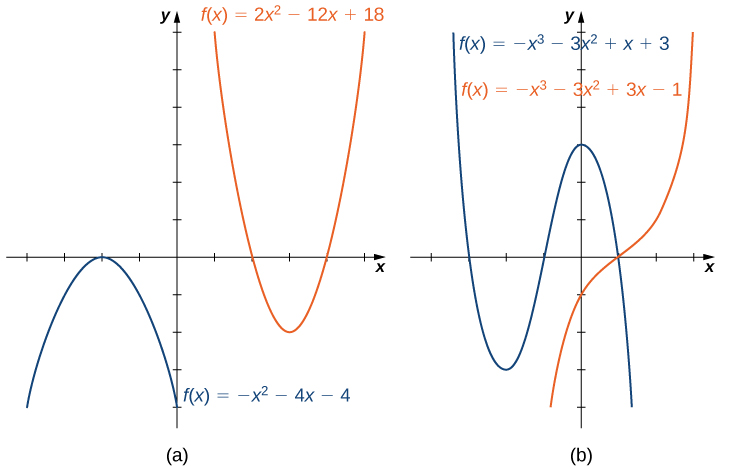
\includegraphics[width=\linewidth]{external/CNX_Calc_Figure_01_02_005.jpg}
\end{image}%
\tcblower
\end{figureptx}%
\end{subsubsectionptx}
%
%
\typeout{************************************************}
\typeout{Subsubsection 1.2.2.3 Zeros of Polynomial Functions}
\typeout{************************************************}
%
\begin{subsubsectionptx}{Zeros of Polynomial Functions}{}{Zeros of Polynomial Functions}{}{}{g:subsubsection:idm1622018024}
Another characteristic of the graph of a polynomial function is where it intersects the \(x\)-axis. To determine where a function \(f\) intersects the \(x\)-axis, we need to solve the equation \(f(x)= 0 \) for the case of the linear function \(f(x)=mx+b,\) the \(x\)-intercept is given by solving the equation \(mx+b= 0 .\) In this case, we see that the \(x\)-intercept is given by \((-b/m, 0 ).\) In the case of a quadratic function, finding the \(x\)-intercept(s) requires finding the zeros of a quadratic equation: \(ax^2 +bx+c= 0 .\) In some cases, it is easy to factor the polynomial \(ax^2+bx+c\) to find the zeros. If not, we make use of the quadratic formula.%
\begin{note}{Rule: The Quadratic Formula.}{g:note:idm1622007272}%
Consider the quadratic equation%
%
\begin{equation*}
ax^2 +bx+c= 0 ,
\end{equation*}
where \(a\neq  0 .\) The solutions of this equation are given by the quadratic formula%
%
\begin{equation*}
x=\frac{-b\pm \sqrt{b^2- 4 ac}}{ 2 a}.
\end{equation*}
If the discriminant \(b^2- 4 ac\gt  0 ,\) this formula tells us there are two real numbers that satisfy the quadratic equation. If \(b^2- 4 ac= 0 ,\) this formula tells us there is only one solution, and it is a real number. If \(b^2- 4 ac\lt  0 ,\) no real numbers satisfy the quadratic equation.%
\end{note}
In the case of higher-degree polynomials, it may be more complicated to determine where the graph intersects the \(x\)-axis. In some instances, it is possible to find the \(x\)-intercepts by factoring the polynomial to find its zeros. In other cases, it is impossible to calculate the exact values of the \(x\)-intercepts. However, as we see later in the text, in cases such as this, we can use analytical tools to approximate (to a very high degree) where the \(x\)-intercepts are located. Here we focus on the graphs of polynomials for which we can calculate their zeros explicitly.%
\begin{example}{Graphing Polynomial Functions.}{g:example:idm1622004456}%
For the following functions a. and b., i. describe the behavior of \(f(x)\) as \(x\to \pm\infty,\) ii. find all zeros of \(f,\) and iii. sketch a graph of \(f.\)%
%
\begin{enumerate}
\item{}\(\displaystyle f(x)= -2 x^2 + 4 x- 1 \)%
\item{}\(\displaystyle f(x)=x^3 - 3 x^2 - 4 x\)%
\end{enumerate}
\par\smallskip%
\noindent\textbf{\blocktitlefont Solution}.\hypertarget{g:solution:idm1622000872}{}\quad{}%
\begin{enumerate}
\item{}The function \(f(x)= -2 x^2 + 4 x- 1 \) is a quadratic function.%
%
\begin{enumerate}
\item{}Because \(a= -2 \lt  0 ,\text{ as } x\to \pm\infty,f(x)\to -\infty.\)%
\item{}To find the zeros of \(f,\) use the quadratic formula. The zeros are%
\begin{equation*}
x= \frac{ -4 \pm \sqrt{ 4^2- 4 ( -2 )( -1 )}}{ 2 ( -2 )}= \frac{ -4 \pm \sqrt{ 8 }}{ -4 }= \frac{ -4 \pm  2 \sqrt{ 2 }}{ -4 }=\frac{ 2 \pm \sqrt{ 2 }}{ 2 }.
\end{equation*}
%
\item{}To sketch the graph of \(f,\) use the information from your previous answers and combine it with the fact that the graph is a parabola opening downward.%
\begin{image}{0.25}{0.5}{0.25}%
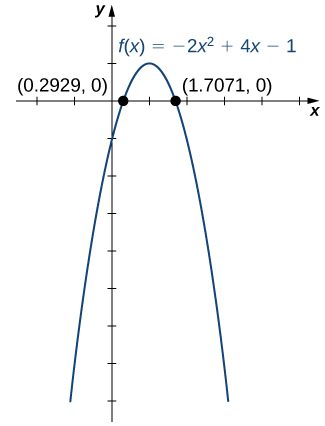
\includegraphics[width=\linewidth]{external/CNX_Calc_Figure_01_02_006.jpg}
\end{image}%
\end{enumerate}
\item{}The function \(f(x)=x^3 - 3 x^2 - 4 x\) is a cubic function.%
%
\begin{enumerate}
\item{}Because \(a= 1 \gt  0 ,\text{ as } x\to \infty,f(x)\to \infty.\) As \(x\to -\infty,f(x)\to -\infty.\)%
\item{}To find the zeros of \(f,\) we need to factor the polynomial. First, when we factor \(x\) out of all the terms, we find%
\begin{equation*}
f(x)=x(x^2 - 3 x- 4 ).
\end{equation*}
 Then, when we factor the quadratic function \(x^2 - 3 x- 4 ,\) we find%
\begin{equation*}
f(x)=x(x- 4 )(x+ 1 ).
\end{equation*}
 Therefore, the zeros of \(f\) are \(x= 0 , 4 , -1 .\)%
\item{}Combining the results from parts i. and ii., draw a rough sketch of \(f.\) \begin{image}{0.25}{0.5}{0.25}%
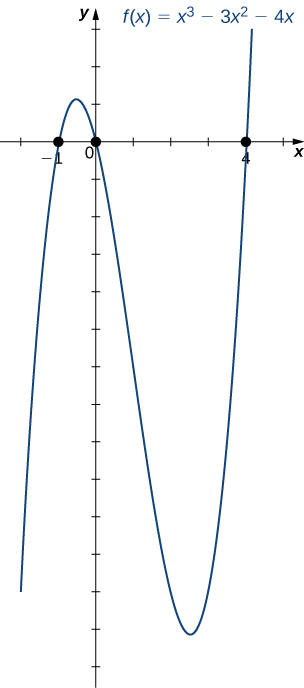
\includegraphics[width=\linewidth]{external/CNX_Calc_Figure_01_02_007.jpg}
\end{image}%
%
\end{enumerate}
\end{enumerate}
\end{example}
\begin{inlineexercise}{}{g:exercise:idm1621986664}%
Consider the quadratic function \(f(x)= 3 x^2 - 6 x+ 2 .\) Find the zeros of \(f.\) Does the parabola open upward or downward?%
\par\smallskip%
\noindent\textbf{\blocktitlefont Hint}.\hypertarget{g:hint:idm1621982824}{}\quad{}Use the quadratic formula.%
\par\smallskip%
\noindent\textbf{\blocktitlefont Solution}.\hypertarget{g:solution:idm1621984616}{}\quad{}The zeros are \(x= 1 \pm \sqrt{ 3 } / 3 .\) The parabola opens upward.%
\end{inlineexercise}%
\end{subsubsectionptx}
\end{subsectionptx}
%
%
\typeout{************************************************}
\typeout{Subsection 1.2.3 Algebraic Functions}
\typeout{************************************************}
%
\begin{subsectionptx}{Algebraic Functions}{}{Algebraic Functions}{}{}{g:subsection:idm1622054760}
By allowing for quotients and fractional powers in polynomial functions, we create a larger class of functions. An \terminology{algebraic function} is one that involves addition, subtraction, multiplication, division, rational powers, and roots. Two types of algebraic functions are rational functions and root functions.%
\par
Just as rational numbers are quotients of integers, rational functions are quotients of polynomials. In particular, a \terminology{rational function} is any function of the form \(f(x)=p(x) /q(x),\) where \(p(x)\) and \(q(x)\) are polynomials. For example,%
%
\begin{equation*}
f(x)= \frac{ 3 x- 1}{  5 x+ 2 } \text{ and } g(x)=\frac{ 4}{x^2 + 1 }
\end{equation*}
are rational functions. A \terminology{root function} is a power function of the form \(f(x)= x^{1/n},\) where \(n\) is a positive integer greater than one. For example, \(f(x)=x^{1/2}=\sqrt{x}\) is the square-root function and \(g(x)=x^{1/3}=\sqrt[3]{x}\) is the cube-root function. By allowing for compositions of root functions and rational functions, we can create other algebraic functions. For example, \(f(x)=\sqrt{ 4 -x^2 }\) is an algebraic function.%
\begin{example}{Finding Domain and Range for Algebraic Functions.}{g:example:idm1621977192}%
For each of the following functions, find the domain and range.%
%
\begin{enumerate}
\item{}\(\displaystyle f(x)=\frac{ 3 x- 1}{ 5 x+ 2 }\)%
\item{}To find the domain of \(f\), we need \(4 –x^2 \geq  0 \). Or, \(4 \geq x^2 \) Or \(x^2 \leq   4 \), the solution to which is \(– 2 \leq  x\leq   2 \). Therefore, the domain is \({x|– 2 \leq  x\leq   2 }\). If \(– 2 \leq  x\leq   2 \), then \(0 \leq   4 –x^2 \leq   4 \). Therefore, \(0 \leq  \sqrt{ 4 –x^2 }\leq   2 \) and the range of \(f\) is \({y| 0 \leq  x\leq   2 }\).%
\end{enumerate}
\par\smallskip%
\noindent\textbf{\blocktitlefont Solution}.\hypertarget{g:solution:idm1621970152}{}\quad{}%
\begin{enumerate}
\item{}It is not possible to divide by zero, so the domain is the set of real numbers \(x\) such that \(x\neq - 2  / 5 .\) To find the range, we need to find the values \(y\) for which there exists a real number \(x\) such that%
\begin{equation*}
y=\frac{ 3 x- 1}{ 5 x+ 2 }.
\end{equation*}
When we multiply both sides of this equation by \(5 x+ 2 ,\) we see that \(x\) must satisfy the equation%
\begin{equation*}
5 xy+ 2 y= 3 x- 1 .
\end{equation*}
From this equation, we can see that \(x\) must satisfy%
%
\begin{equation*}
2 y+ 1 =x( 3 - 5 y).
\end{equation*}
If \(y= 3  / 5 ,\) this equation has no solution. On the other hand, as long as \(y\neq  3  / 5 ,\)%
\begin{equation*}
x=\frac{ 2 y+ 1 }{ 3 - 5 y}
\end{equation*}
satisfies this equation. We can conclude that the range of \(f\) is \({y|y\neq  3  / 5 }.\)%
\item{}To find the domain of \(f,\) we need \(4 -x^2 \geq  0 .\) When we factor, we write \(4 -x^2 =( 2 -x)( 2 +x)\geq  0 .\) This inequality holds if and only if both terms are positive or both terms are negative. For both terms to be positive, we need to find \(x\) such that%
\begin{equation*}
2 -x\geq  0  \text{ and }  2 +x\geq  0 .
\end{equation*}
These two inequalities reduce to \(2 \geq x\) and \(x\geq  -2 .\) Therefore, the set \({x|- 2 \leq  x\leq   2 }\) must be part of the domain. For both terms to be negative, we need%
\begin{equation*}
2 -x\leq   0  \text{ and }  2 +x\geq  0 .
\end{equation*}
These two inequalities also reduce to \(2 \leq  x\) and \(x\geq  -2 .\) There are no values of \(x\) that satisfy both of these inequalities. Thus, we can conclude the domain of this function is \({x|- 2 \leq  x\leq   2 }.\) If \(-2 \leq  x\leq   2 ,\) then \(0 \leq   4 -x^2 \leq   4 .\) Therefore, \(0 \leq  \sqrt{ 4 -x^2 }\leq   2 ,\) and the range of \(f\) is \({y| 0 \leq  y\leq   2 }.\)%
\end{enumerate}
\end{example}
\begin{inlineexercise}{}{g:exercise:idm1621953000}%
Find the domain and range for the function \(f(x)=( 5 x+ 2 ) /( 2 x- 1 ).\)%
\par\smallskip%
\noindent\textbf{\blocktitlefont Hint}.\hypertarget{g:hint:idm1621949928}{}\quad{}The denominator cannot be zero. Solve the equation \(y=( 5 x+ 2 ) /( 2 x- 1 )\) for \(x\) to find the range.%
\par\smallskip%
\noindent\textbf{\blocktitlefont Solution}.\hypertarget{g:solution:idm1621950824}{}\quad{}The domain is the set of real numbers \(x\) such that \(x\neq  1  / 2 .\) The range is the set \({y|y\neq  5  / 2 }.\)%
\end{inlineexercise}%
The root functions \(f(x)= x^{1/n}\) have defining characteristics depending on whether \(n\) is odd or even. For all even integers \(n\geq  2 ,\) the domain of \(f(x)= x^{1/n}\) is the interval \([ 0 ,\infty).\) For all odd integers \(n\geq  1 ,\) the domain of \(f(x)= x^{1/n}\) is the set of all real numbers. Since \(x^{1/n}=-(-x)^{1/n}\) for odd integers \(n,f(x)= x^{1/n}\) is an odd function if \(n\) is odd. See the graphs of root functions for different values of \(n\) in \hyperref[x:figure:CNX_Calc_Figure_01_02_022]{Figure~{\xreffont\ref{x:figure:CNX_Calc_Figure_01_02_022}}}.%
\begin{figureptx}{(a) If \(n\) is even, the domain of \(f(x)= \sqrt[n]{x}\) is \([ 0 ,\infty).\) (b) If \(n\) is odd, the domain of \(f(x)= \sqrt[n]{x}\) is \((-\infty,\infty)\) and the function \(f(x)= \sqrt[n]{x}\) is an odd function.}{x:figure:CNX_Calc_Figure_01_02_022}{}%
\begin{image}{0.25}{0.5}{0.25}%
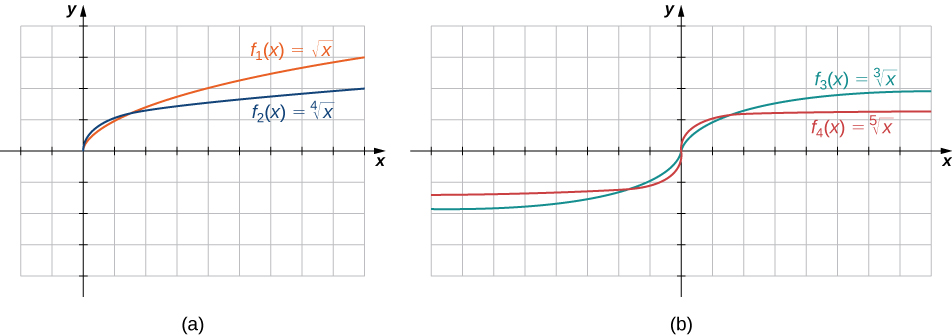
\includegraphics[width=\linewidth]{external/CNX_Calc_Figure_01_02_022.jpg}
\end{image}%
\tcblower
\end{figureptx}%
\begin{example}{Finding Domains for Algebraic Functions.}{g:example:idm1621939048}%
For each of the following functions, determine the domain of the function.%
%
\begin{enumerate}
\item{}\(\displaystyle f(x)=\frac{ 3}{ x^2 - 1 }\)%
\item{}\(\displaystyle f(x)=\frac{ 2 x+ 5}{ 3 x^2 + 4 }\)%
\item{}\(\displaystyle f(x)=\sqrt{ 4 - 3 x}\)%
\item{}\(\displaystyle f(x)=\sqrt[3]{2 x- 1}\)%
\end{enumerate}
\par\smallskip%
\noindent\textbf{\blocktitlefont Solution}.\hypertarget{g:solution:idm1621935208}{}\quad{}%
\begin{enumerate}
\item{}You cannot divide by zero, so the domain is the set of values \(x\) such that \(x^2 - 1 \neq  0 .\) Therefore, the domain is \({x|x\neq \pm 1 }.\)%
\item{}You need to determine the values of \(x\) for which the denominator is zero. Since \(3 x^2 + 4 \geq  4 \) for all real numbers \(x,\) the denominator is never zero. Therefore, the domain is \((-\infty,\infty).\)%
\item{}Since the square root of a negative number is not a real number, the domain is the set of values \(x\) for which \(4 - 3 x\geq  0 .\) Therefore, the domain is \({x|x\leq   4  / 3 }.\)%
\item{}The cube root is defined for all real numbers, so the domain is the interval \((-\infty,\infty)\)%
\end{enumerate}
\end{example}
\begin{inlineexercise}{}{g:exercise:idm1621930472}%
Find the domain for each of the following functions: \(f(x)=( 5 - 2 x) /(x^2 + 2 )\) and \(g(x)=\sqrt{ 5 x- 1 }.\)%
\par\smallskip%
\noindent\textbf{\blocktitlefont Hint}.\hypertarget{g:hint:idm1621930600}{}\quad{}Determine the values of \(x\) when the expression in the denominator of \(f\) is nonzero, and find the values of \(x\) when the expression inside the radical of \(g\) is nonnegative.%
\par\smallskip%
\noindent\textbf{\blocktitlefont Solution}.\hypertarget{g:solution:idm1621924840}{}\quad{}The domain of \(f\) is \((-\infty,\infty)\) The domain of \(g\) is \({x|x\geq  1  / 5 }.\)%
\end{inlineexercise}%
\end{subsectionptx}
%
%
\typeout{************************************************}
\typeout{Subsection 1.2.4 Transcendental Functions}
\typeout{************************************************}
%
\begin{subsectionptx}{Transcendental Functions}{}{Transcendental Functions}{}{}{g:subsection:idm1621925352}
Thus far, we have discussed algebraic functions. Some functions, however, cannot be described by basic algebraic operations. These functions are known as \terminology{transcendental functions} because they are said to “transcend,” or go beyond, algebra. The most common transcendental functions are  exponential  and logarithmic functions. An exponential function is a function of the form \(f(x)=b^x,\) where the base \(b\gt  0 ,b\neq  1 .\) A \terminology{logarithmic function} is a function of the form \(f(x)=\log_b(x)\) for some constant \(b\gt  0 ,b\neq  1 ,\) where \(\log_b(x)=y\) if and only if \(b^y=x.\) (We also discuss exponential and logarithmic functions later in the chapter.)%
\begin{example}{Classifying Algebraic and Transcendental Functions.}{g:example:idm1621919336}%
Classify each of the following functions, a. through c., as algebraic or transcendental.%
%
\begin{enumerate}
\item{}\(\displaystyle f(x)=\frac{\sqrt{x^3 + 1 }}{ 4 x+ 2 }\)%
\item{}\(\displaystyle f(x)=2^{x^2}\)%
\item{}\(\displaystyle f(x)=\ln(2x) \)%
\end{enumerate}
\par\smallskip%
\noindent\textbf{\blocktitlefont Solution}.\hypertarget{g:solution:idm1621916776}{}\quad{}%
\begin{enumerate}
\item{}Since this function involves basic algebraic operations only, it is an algebraic function.%
\item{}This function cannot be written as a formula that involves only basic algebraic operations, so it is transcendental. (Note that algebraic functions can only have powers that are rational numbers.)%
\item{}As in part b., this function cannot be written using a formula involving basic algebraic operations only; therefore, this function is transcendental.%
\end{enumerate}
\end{example}
\begin{inlineexercise}{}{g:exercise:idm1621920232}%
Is \(f(x)=x / 2 \) an algebraic or a transcendental function?%
\par\smallskip%
\noindent\textbf{\blocktitlefont Solution}.\hypertarget{g:solution:idm1621914216}{}\quad{}Algebraic%
\end{inlineexercise}%
\end{subsectionptx}
%
%
\typeout{************************************************}
\typeout{Subsection 1.2.5 Piecewise-Defined Functions}
\typeout{************************************************}
%
\begin{subsectionptx}{Piecewise-Defined Functions}{}{Piecewise-Defined Functions}{}{}{g:subsection:idm1621915112}
Sometimes a function is defined by different formulas on different parts of its domain. A function with this property is known as a \terminology{piecewise-defined function}. The absolute value function is an example of a piecewise-defined function because the formula changes with the sign of \(x\):%
%
\begin{equation*}
f(x)=\begin{cases}x \amp x \lt 0 \\ x \amp x \geq 0\end{cases}\text{.}
\end{equation*}
Other piecewise-defined functions may be represented by completely different formulas, depending on the part of the domain in which a point falls. To graph a piecewise-defined function, we graph each part of the function in its respective domain, on the same coordinate system. If the formula for a function is different for \(x\lt a\) and \(x\gt a,\) we need to pay special attention to what happens at \(x=a\) when we graph the function. Sometimes the graph needs to include an open or closed circle to indicate the value of the function at \(x=a.\) We examine this in the next example.%
\begin{example}{Graphing a Piecewise-Defined Function.}{g:example:idm1621910248}%
Sketch a graph of the following piecewise-defined function:%
%
\begin{equation*}
f(x)=\begin{cases}x+ 3 \amp x\lt  1 \\(x- 2 )^2 \amp x\geq  1 \end{cases}.
\end{equation*}
\par\smallskip%
\noindent\textbf{\blocktitlefont Solution}.\hypertarget{g:solution:idm1621908968}{}\quad{}Graph the linear function \(y=x+ 3 \) on the interval \((-\infty, 1 )\) and graph the quadratic function \(y=(x- 2 )^2\) on the interval \([ 1 ,\infty).\) Since the value of the function at \(x= 1 \) is given by the formula \(f(x)=(x- 2 )^2,\) we see that \(f( 1 )= 1 .\) To indicate this on the graph, we draw a closed circle at the point \(( 1 , 1 ).\) The value of the function is given by \(f(x)=x+ 2 \) for all \(x\lt  1 ,\) but not at \(x= 1 .\) To indicate this on the graph, we draw an open circle at \(( 1 , 4 ).\)%
\begin{figureptx}{This piecewise-defined function is linear for \(x\lt  1 \) and quadratic for \(x\geq  1 .\)}{x:figure:CNX_Calc_Figure_01_02_011}{}%
\begin{image}{0.25}{0.5}{0.25}%
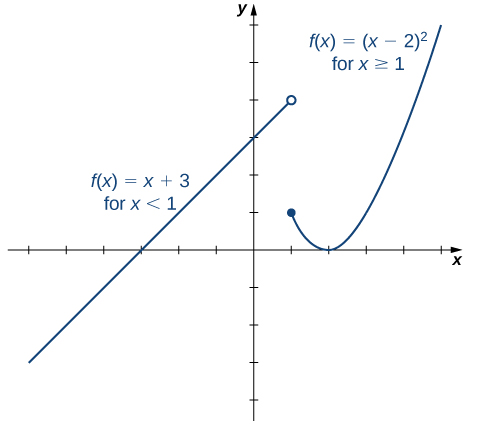
\includegraphics[width=\linewidth]{external/CNX_Calc_Figure_01_02_011.jpg}
\end{image}%
\tcblower
\end{figureptx}%
\end{example}
\begin{inlineexercise}{}{g:exercise:idm1621901672}%
Sketch a graph of the function%
%
\begin{equation*}
f(x)=\begin{cases}2 -x \amp x\leq   2 \\ x+ 2  \amp x\gt  2 .\end{cases}
\end{equation*}
\par\smallskip%
\noindent\textbf{\blocktitlefont Hint}.\hypertarget{g:hint:idm1621900136}{}\quad{}Graph one linear function for \(x\leq   2 \) and then graph a different linear function for \(x\gt  2 .\)%
\par\smallskip%
\noindent\textbf{\blocktitlefont Solution}.\hypertarget{g:solution:idm1621898728}{}\quad{}\begin{image}{0.25}{0.5}{0.25}%
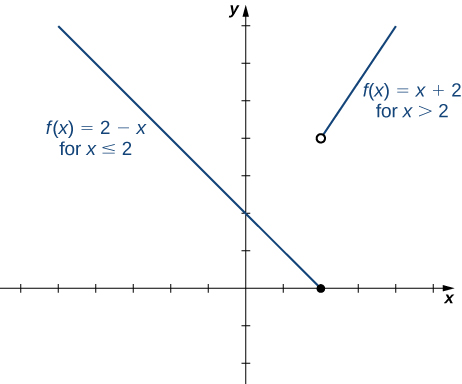
\includegraphics[width=\linewidth]{external/CNX_Calc_Figure_01_02_012.jpg}
\end{image}%
%
\end{inlineexercise}%
\begin{example}{Parking Fees Described by a Piecewise-Defined Function.}{g:example:idm1621898216}%
In a big city, drivers are charged variable rates for parking in a parking garage. They are charged \textdollar{}10 for the first hour or any part of the first hour and an additional \textdollar{}2 for each hour or part thereof up to a maximum of \textdollar{}30 for the day. The parking garage is open from 6 a.m. to 12 midnight.%
%
\begin{enumerate}
\item{}Write a piecewise-defined function that describes the cost \(C\) to park in the parking garage as a function of hours parked \(x.\)%
\item{}Sketch a graph of this function \(C(x).\)%
\end{enumerate}
\par\smallskip%
\noindent\textbf{\blocktitlefont Solution}.\hypertarget{g:solution:idm1621891816}{}\quad{}%
\begin{enumerate}
\item{}Since the parking garage is open 18 hours each day, the domain for this function is \(\{x| 0 \lt x\leq   18 \}.\) The cost to park a car at this parking garage can be described piecewise by the function%
\begin{equation*}
C(x)=\begin{cases} 10 \amp 0 \lt x\leq   1 \\ 12 \amp 1 \lt x\leq   2 \\ 14 \amp 2 \lt x\leq   3 \\ 16 \amp 3 \lt x\leq   4 \\ \vdots \\ 30 \amp 10 \lt x\leq   18 \end{cases}.
\end{equation*}
%
\item{}The graph of the function consists of several horizontal line segments. \begin{image}{0.25}{0.5}{0.25}%
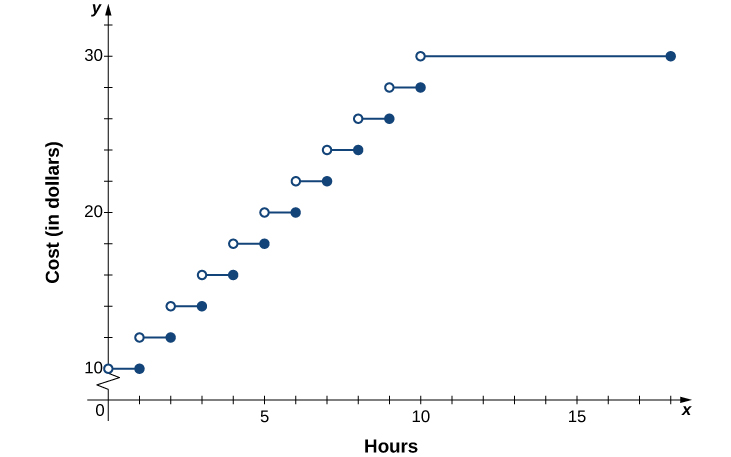
\includegraphics[width=\linewidth]{external/CNX_Calc_Figure_01_02_013.jpg}
\end{image}%
%
\end{enumerate}
\end{example}
\begin{inlineexercise}{}{g:exercise:idm1621892456}%
The cost of mailing a letter is a function of the weight of the letter. Suppose the cost of mailing a letter is \(49 \text{ cents }\) for the first ounce and \(21 \text{ cents }\) for each additional ounce. Write a piecewise-defined function describing the cost \(C\) as a function of the weight \(x\) for \(0 \lt x\leq   3 ,\) where \(C\) is measured in cents and \(x\) is measured in ounces.%
\par\smallskip%
\noindent\textbf{\blocktitlefont Hint}.\hypertarget{g:hint:idm1621890408}{}\quad{}The piecewise-defined function is constant on the intervals \(( 0 , 1 ],( 1 , 2 ],\dots.\)%
\par\smallskip%
\noindent\textbf{\blocktitlefont Solution}.\hypertarget{g:solution:idm1621891048}{}\quad{}\(C(x)=\begin{cases} 49 \amp 0 \lt x\leq   1 \\ 70 \amp 1 \lt x\leq   2 \\ 91 \amp 2 \lt x\leq   3 \end{cases}\)%
\end{inlineexercise}%
\end{subsectionptx}
%
%
\typeout{************************************************}
\typeout{Subsection 1.2.6 Transformations of Functions}
\typeout{************************************************}
%
\begin{subsectionptx}{Transformations of Functions}{}{Transformations of Functions}{}{}{g:subsection:idm1621884008}
We have seen several cases in which we have added, subtracted, or multiplied constants to form variations of simple functions. In the previous example, for instance, we subtracted 2 from the argument of the function \(y=x^2 \) to get the function \(f(x)=(x- 2 )^2.\) This subtraction represents a shift of the function \(y=x^2 \) two units to the right. A shift, horizontally or vertically, is a type of \terminology{transformation of a function}. Other transformations include horizontal and vertical scalings, and reflections about the axes.%
\par
A vertical shift of a function occurs if we add or subtract the same constant to each output \(y.\) For \(c\gt  0 ,\) the graph of \(f(x)+c\) is a shift of the graph of \(f(x)\) up \(c\) units, whereas the graph of \(f(x)-c\) is a shift of the graph of \(f(x)\) down \(c\) units. For example, the graph of the function \(f(x)=x^3 + 4 \) is the graph of \(y=x^3 \) shifted up \(4 \) units; the graph of the function \(f(x)=x^3 - 4 \) is the graph of \(y=x^3 \) shifted down \(4 \) units (\hyperref[x:figure:CNX_Calc_Figure_01_02_023]{Figure~{\xreffont\ref{x:figure:CNX_Calc_Figure_01_02_023}}}).%
\begin{figureptx}{(a) For \(c\gt  0 ,\) the graph of \(y=f(x)+c\) is a vertical shift up \(c\) units of the graph of \(y=f(x).\) (b) For \(c\gt  0 ,\) the graph of \(y=f(x)-c\) is a vertical shift down \(c\) units of the graph of \(y=f(x).\)}{x:figure:CNX_Calc_Figure_01_02_023}{}%
\begin{image}{0.25}{0.5}{0.25}%
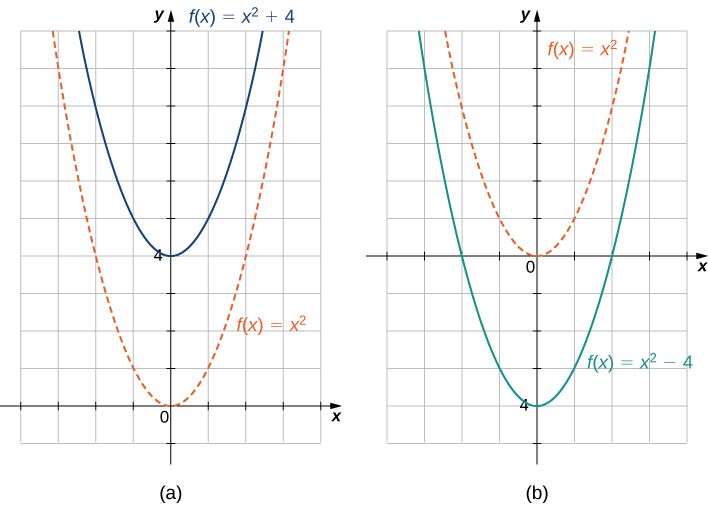
\includegraphics[width=\linewidth]{external/CNX_Calc_Figure_01_02_023.jpg}
\end{image}%
\tcblower
\end{figureptx}%
A horizontal shift of a function occurs if we add or subtract the same constant to each input \(x.\) For \(c\gt  0 ,\) the graph of \(f(x+c)\) is a shift of the graph of \(f(x)\) to the left \(c\) units; the graph of \(f(x-c)\) is a shift of the graph of \(f(x)\) to the right \(c\) units. Why does the graph shift left when adding a constant and shift right when subtracting a constant? To answer this question, let’s look at an example.%
\par
Consider the function \(f(x)=|x+ 3 |\) and evaluate this function at \(x- 3 .\) Since \(f(x- 3 )=|x|\) and \(x- 3 \lt x,\) the graph of \(f(x)=|x+ 3 |\) is the graph of \(y=|x|\) shifted left 3 units. Similarly, the graph of \(f(x)=|x- 3 |\) is the graph of \(y=|x|\) shifted right \(3 \) units (\hyperref[x:figure:CNX_Calc_Figure_01_02_015]{Figure~{\xreffont\ref{x:figure:CNX_Calc_Figure_01_02_015}}}).%
\begin{figureptx}{(a) For \(c\gt  0 ,\) the graph of \(y=f(x+c)\) is a horizontal shift left \(c\) units of the graph of \(y=f(x).\) (b) For \(c\gt  0 ,\) the graph of \(y=f(x-c)\) is a horizontal shift right \(c\) units of the graph of \(y=f(x).\)}{x:figure:CNX_Calc_Figure_01_02_015}{}%
\begin{image}{0.25}{0.5}{0.25}%
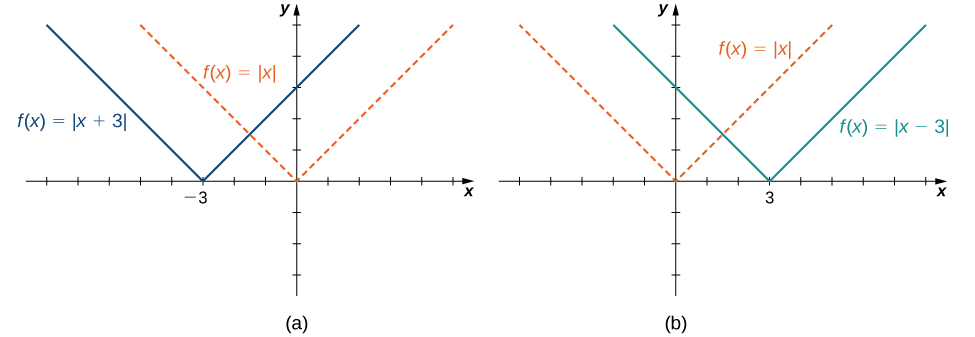
\includegraphics[width=\linewidth]{external/CNX_Calc_Figure_01_02_015.jpg}
\end{image}%
\tcblower
\end{figureptx}%
A vertical scaling of a graph occurs if we multiply all outputs \(y\) of a function by the same positive constant. For \(c\gt  0 ,\) the graph of the function \(cf(x)\) is the graph of \(f(x)\) scaled vertically by a factor of \(c.\) If \(c\gt  1 ,\) the values of the outputs for the function \(cf(x)\) are larger than the values of the outputs for the function \(f(x);\) therefore, the graph has been stretched vertically. If \(0 \lt c\lt  1 ,\) then the outputs of the function \(cf(x)\) are smaller, so the graph has been compressed. For example, the graph of the function \(f(x)= 3 x^2 \) is the graph of \(y=x^2 \) stretched vertically by a factor of 3, whereas the graph of \(f(x)=x^2  / 3 \) is the graph of \(y=x^2 \) compressed vertically by a factor of \(3 \) (\hyperref[x:figure:CNX_Calc_Figure_01_02_024]{Figure~{\xreffont\ref{x:figure:CNX_Calc_Figure_01_02_024}}}).%
\begin{figureptx}{(a) If \(c\gt  1 ,\) the graph of \(y=cf(x)\) is a vertical stretch of the graph of \(y=f(x).\) (b) If \(0 \lt c\lt  1 ,\) the graph of \(y=cf(x)\) is a vertical compression of the graph of \(y=f(x).\)}{x:figure:CNX_Calc_Figure_01_02_024}{}%
\begin{image}{0.25}{0.5}{0.25}%
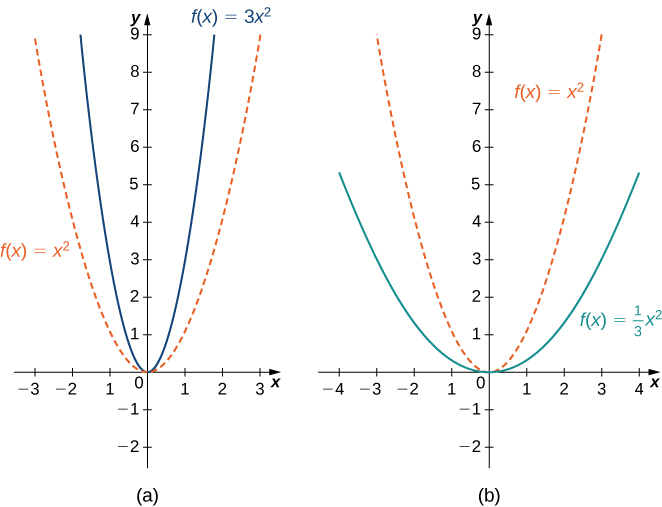
\includegraphics[width=\linewidth]{external/CNX_Calc_Figure_01_02_024.jpg}
\end{image}%
\tcblower
\end{figureptx}%
The horizontal scaling of a function occurs if we multiply the inputs \(x\) by the same positive constant. For \(c\gt  0 ,\) the graph of the function \(f(cx)\) is the graph of \(f(x)\) scaled horizontally by a factor of \(c.\) If \(c\gt  1 ,\) the graph of \(f(cx)\) is the graph of \(f(x)\) compressed horizontally. If \(0 \lt c\lt  1 ,\) the graph of \(f(cx)\) is the graph of \(f(x)\) stretched horizontally. For example, consider the function \(f(x)=\sqrt{ 2 x}\) and evaluate \(f\) at \(x / 2 .\) Since \(f(x / 2 )=\sqrt{x},\) the graph of \(f(x)=\sqrt{ 2 x}\) is the graph of \(y=\sqrt{x}\) compressed horizontally. The graph of \(y=\sqrt{x / 2 }\) is a horizontal stretch of the graph of \(y=\sqrt{x}\) (\hyperref[x:figure:CNX_Calc_Figure_01_02_017]{Figure~{\xreffont\ref{x:figure:CNX_Calc_Figure_01_02_017}}}).%
\begin{figureptx}{(a) If \(c\gt  1 ,\) the graph of \(y=f(cx)\) is a horizontal compression of the graph of \(y=f(x).\) (b) If \(0 \lt c\lt  1 ,\) the graph of \(y=f(cx)\) is a horizontal stretch of the graph of \(y=f(x).\)}{x:figure:CNX_Calc_Figure_01_02_017}{}%
\begin{image}{0.25}{0.5}{0.25}%
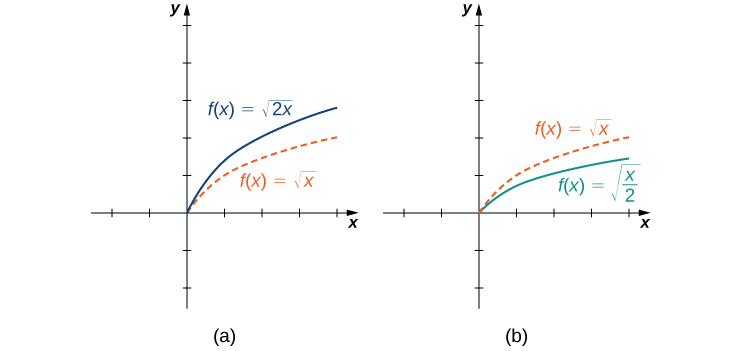
\includegraphics[width=\linewidth]{external/CNX_Calc_Figure_01_02_017.jpg}
\end{image}%
\tcblower
\end{figureptx}%
We have explored what happens to the graph of a function \(f\) when we multiply \(f\) by a constant \(c\gt  0 \) to get a new function \(cf(x).\) We have also discussed what happens to the graph of a function \(f\) when we multiply the independent variable \(x\) by \(c\gt  0 \) to get a new function \(f(cx).\) However, we have not addressed what happens to the graph of the function if the constant \(c\) is negative. If we have a constant \(c\lt  0 ,\) we can write \terminology{c} as a positive number multiplied by \(-1 ;\) but, what kind of transformation do we get when we multiply the function or its argument by \(-1 ?\) When we multiply all the outputs by \(-1 ,\) we get a reflection about the \(x\)-axis. When we multiply all inputs by \(-1 ,\) we get a reflection about the \(y\)-axis. For example, the graph of \(f(x)=-(x^3 + 1 )\) is the graph of \(y=(x^3 + 1 )\) reflected about the \(x\)-axis. The graph of \(f(x)=(-x)^3>+ 1 \) is the graph of \(y=x^3 + 1 \) reflected about the \(y\)-axis (\hyperref[x:figure:CNX_Calc_Figure_01_02_018]{Figure~{\xreffont\ref{x:figure:CNX_Calc_Figure_01_02_018}}}).%
\begin{figureptx}{(a) The graph of \(y=-f(x)\) is the graph of \(y=f(x)\) reflected about the \(x\)-axis. (b) The graph of \(y=f(-x)\) is the graph of \(y=f(x)\) reflected about the\(y\)-axis.}{x:figure:CNX_Calc_Figure_01_02_018}{}%
\begin{image}{0.25}{0.5}{0.25}%
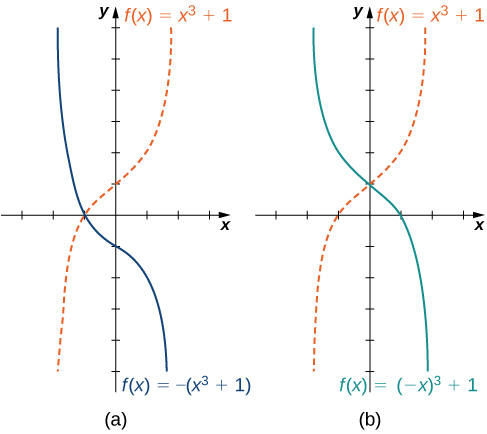
\includegraphics[width=\linewidth]{external/CNX_Calc_Figure_01_02_018.jpg}
\end{image}%
\tcblower
\end{figureptx}%
If the graph of a function consists of more than one transformation of another graph, it is important to transform the graph in the correct order. Given a function \(f(x),\) the graph of the related function \(y=cf(a(x+b))+d\) can be obtained from the graph of \(y=f(x)\) by performing the transformations in the following order.%
%
\begin{enumerate}
\item{}Horizontal shift of the graph of \(y=f(x).\) If \(b\gt  0 ,\) shift left. If \(b\lt  0 ,\) shift right.%
\item{}Horizontal scaling of the graph of \(y=f(x+b)\) by a factor of \(|a|.\) If \(a\lt  0 ,\) reflect the graph about the \(y\)-axis.%
\item{}Vertical scaling of the graph of \(y=f(a(x+b))\) by a factor of \(|c|.\) If \(c\lt  0 ,\) reflect the graph about the \(x\)-axis.%
\item{}Vertical shift of the graph of \(y=cf(a(x+b)).\) If \(d\gt  0 ,\) shift up. If \(d\lt  0 ,\) shift down.%
\end{enumerate}
We can summarize the different transformations and their related effects on the graph of a function in the following table.%
\begin{tableptx}{\textbf{Transformations of Functions}}{x:table:fs-id1170573580486}{}%
\centering%
{\tabularfont%
\begin{tabular}{ll}
\textbf{Transformation of \(f(c\gt  0 )\)}&\textbf{Effect on the graph of \(f\)}\tabularnewline[0pt]
\(f(x)+c\)&Vertical shift up \(c\) units\tabularnewline[0pt]
\(f(x)-c\)&Vertical shift down \(c\) units\tabularnewline[0pt]
\(f(x+c)\)&Shift left by \(c\) units\tabularnewline[0pt]
\(f(x-c)\)&Shift right by \(c\) units\tabularnewline[0pt]
\(cf(x)\)&Vertical stretch if \(c\gt  1 ;\)vertical compression if \(0 \lt c\lt  1 \)\tabularnewline[0pt]
\(f(cx)\)&Horizontal stretch if \(0 \lt c\lt  1 ;\) horizontal compression if \(c\gt  1 \)\tabularnewline[0pt]
\(-f(x)\)&Reflection about the \(x\)-axis\tabularnewline[0pt]
\(f(-x)\)&Reflection about the \(y\)-axis
\end{tabular}
}%
\end{tableptx}%
\begin{example}{Transforming a Function.}{g:example:idm1621698152}%
For each of the following functions, a. and b., sketch a graph by using a sequence of transformations of a well-known function.%
%
\begin{enumerate}
\item{}\(\displaystyle f(x)=-|x+ 2 |- 3 \)%
\item{}\(\displaystyle f(x)= 3 \sqrt{-x}+ 1 \)%
\end{enumerate}
\par\smallskip%
\noindent\textbf{\blocktitlefont Solution}.\hypertarget{g:solution:idm1621693160}{}\quad{}%
\begin{enumerate}
\item{}Starting with the graph of \(y=|x|,\) shift \(2 \) units to the left, reflect about the \(x\)-axis, and then shift down 3 units. \begin{figureptx}{The function \(f(x)=-|x+ 2 |- 3 \) can be viewed as a sequence of three transformations of the function \(y=|x|.\)}{x:figure:CNX_Calc_Figure_01_02_019}{}%
\begin{image}{0.25}{0.5}{0.25}%
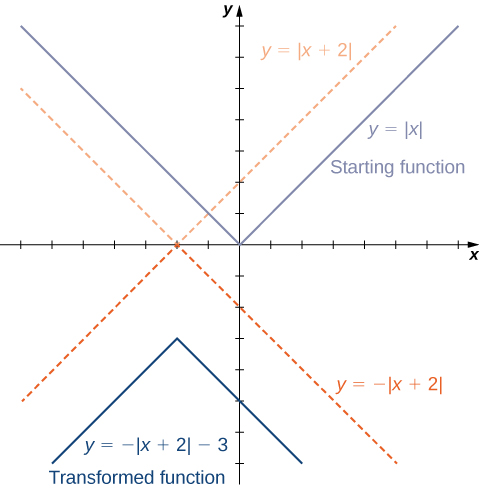
\includegraphics[width=\linewidth]{external/CNX_Calc_Figure_01_02_019.jpg}
\end{image}%
\tcblower
\end{figureptx}%
%
\item{}Starting with the graph of \(y=\sqrt{x},\) reflect about the \(y\)-axis, stretch the graph vertically by a factor of 3, and move up 1 unit. \begin{figureptx}{The function \(f(x)= 3 \sqrt{-x}+ 1 \) can be viewed as a sequence of three transformations of the function \(y=\sqrt{x}.\)}{x:figure:CNX_Calc_Figure_01_02_020}{}%
\begin{image}{0.25}{0.5}{0.25}%
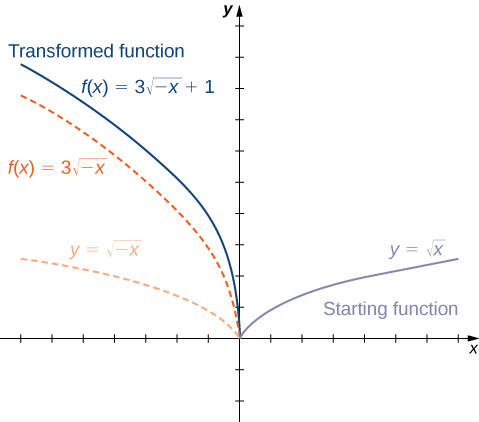
\includegraphics[width=\linewidth]{external/CNX_Calc_Figure_01_02_020.jpg}
\end{image}%
\tcblower
\end{figureptx}%
%
\end{enumerate}
\end{example}
\begin{inlineexercise}{}{g:exercise:idm1621684072}%
Describe how the function \(f(x)=-(x+ 1 )^2- 4 \) can be graphed using the graph of \(y=x^2 \) and a sequence of transformations.%
\par\smallskip%
\noindent\textbf{\blocktitlefont Hint}.\hypertarget{g:hint:idm1621685352}{}\quad{}Use \hyperref[x:table:fs-id1170573580486]{Table~{\xreffont\ref{x:table:fs-id1170573580486}}}.%
\par\smallskip%
\noindent\textbf{\blocktitlefont Solution}.\hypertarget{g:solution:idm1621683304}{}\quad{}Shift the graph \(y=x^2 \) to the left 1 unit, reflect about the \(x\)-axis, then shift down 4 units.%
\end{inlineexercise}%
\end{subsectionptx}
%
%
\typeout{************************************************}
\typeout{Subsection 1.2.7 Key Concepts}
\typeout{************************************************}
%
\begin{subsectionptx}{Key Concepts}{}{Key Concepts}{}{}{g:subsection:idm1621678824}
%
\begin{itemize}[label=\textbullet]
\item{}The power function \(f(x)=x^n\) is an even function if \(n\) is even and \(n\neq  0 ,\) and it is an odd function if \(n\) is odd.%
\item{}The root function \(f(x)=x^{1/n}\) has the domain \([ 0 ,\infty)\) if \(n\) is even and the domain \((-\infty,\infty)\) if \(n\) is odd. If \(n\) is odd, then \(f(x)= x^{1/n}\) is an odd function.%
\item{}The domain of the rational function \(f(x)=p(x) /q(x),\) where \(p(x)\) and \(q(x)\) are polynomial functions, is the set of \(x\) such that \(q(x)\neq  0 .\)%
\item{}Functions that involve the basic operations of addition, subtraction, multiplication, division, and powers are algebraic functions. All other functions are transcendental. Trigonometric, exponential, and logarithmic functions are examples of transcendental functions.%
\item{}A polynomial function \(f\) with degree \(n\geq  1 \) satisfies \(f(x)\to \pm\infty\) as \(x\to \pm\infty.\) The sign of the output as \(x\to \infty\) depends on the sign of the leading coefficient only and on whether \(n\) is even or odd.%
\item{}Vertical and horizontal shifts, vertical and horizontal scalings, and reflections about the \(x\)- and \(y\)-axes are examples of transformations of functions.%
\end{itemize}
\end{subsectionptx}
%
%
\typeout{************************************************}
\typeout{Subsection 1.2.8 Key Equations}
\typeout{************************************************}
%
\begin{subsectionptx}{Key Equations}{}{Key Equations}{}{}{g:subsection:idm1621669224}
%
\begin{itemize}[label=\textbullet]
\item{}Point-slope equation of a line \(y-y_1=m(x-x_1)\)%
\item{}Slope-intercept form of a line \(y=mx+b\)%
\item{}Standard form of a line \(ax+by=c\)%
\item{}Polynomial function \(f(x)=a_nx^n+a_{n-1}x^{n-1}+\cdots+a_1x+a_0\)%
\end{itemize}
\end{subsectionptx}
This book is a custom edition based on OpenStax Calculus Volume 1. You can download the original for free at https:\slash{}\slash{}openstax.org\slash{}details\slash{}books\slash{}calculus-volume-1.%
\end{sectionptx}
%
%
\typeout{************************************************}
\typeout{Section 1.3 Mathematical Modeling}
\typeout{************************************************}
%
\begin{sectionptx}{Mathematical Modeling}{}{Mathematical Modeling}{}{}{x:section:sec_Ch1Sec3}
\begin{introduction}{Learning Objectives.}%
%
\begin{itemize}[label=\textbullet]
\item{}Discuss linear mathematical models for cost, revenue, profit, supply, and demand functions.%
\item{}Find and analyze the break-even quantity and equilibrium point.%
\item{}Discuss quadratic mathematical models.%
\item{}Find and analyze the vertex point of a quadratic function.%
\item{}Optimize cost, revenue, and profit functions.%
\end{itemize}
A large variety of real-world situations can be described using \terminology{mathematical models}. A mathematical model is a method of simulating real-life situations with mathematical equations. Physicists, engineers, economists, and other researchers develop models by combining observation with quantitative data to develop equations, functions, graphs, and other mathematical tools to describe the behavior of various systems accurately. Models are useful because they help predict future outcomes. Examples of mathematical models include the study of population dynamics, investigations of weather patterns, and predictions of product sales.%
\end{introduction}%
%
%
\typeout{************************************************}
\typeout{Subsection 1.3.1 Mathematical Models of Cost, Revenue, and Profit}
\typeout{************************************************}
%
\begin{subsectionptx}{Mathematical Models of Cost, Revenue, and Profit}{}{Mathematical Models of Cost, Revenue, and Profit}{}{}{g:subsection:idm1621661416}
Given \(x\) the number of units produced, the \terminology{cost function} outputs the amount a business or company must pay in order to produce \(x\) units. There are typicically two types of costs: fixed and variable. In a linear cost model, the cost function is expressed as%
%
\begin{equation*}
C(x)=mx+b
\end{equation*}
where \(m\) is the cost per unit also referred to as the \terminology{variable} or \terminology{marginal cost}. Here, the variable cost term \(mx\) depends on the number of units produced. Some examples of variable\slash{}marginal costs are labor, material, or manufacturing costs. Additionally, \(b\) are the \terminology{fixed costs} which is the amount one must pay to operate a business. The fixed cost is independent of the number of units produced. It often represents the amount one must pay if 0 units are produced since \(b\) is the \(y\)-intercept of the cost function. That is, \(C(0)=b\). Some examples of fixed costs are rent, utility bills, or operating costs.%
\par
The \terminology{revenue function} outputs the payment received from selling \(x\) units. In a linear model, the revenue is%
%
\begin{equation*}
R(x)=px
\end{equation*}
where \(p\) is the selling price per unit which is also called the \terminology{marginal revenue}.%
\par
The \terminology{profit function} outputs the net proceeds after paying off the expenses\slash{}costs. That is,%
%
\begin{equation*}
P(x)=R(x)-C(x)\text{.}
\end{equation*}
Notice that the above definition for the profit function holds if either of our revenue or cost functions are non-linear.%
\par
If profits are negative, this is considered a \(loss\) and if profits are positive, this is considered a \(gain\).%
%
%
\typeout{************************************************}
\typeout{Subsubsection 1.3.1.1 Break-even Analysis}
\typeout{************************************************}
%
\begin{subsubsectionptx}{Break-even Analysis}{}{Break-even Analysis}{}{}{g:subsubsection:idm1621649000}
Companies often look for the point at which there is no \(loss\) or \(gain\). This gives you the minimum number of units a company must produce in order to make a profit.%
\begin{definition}{}{g:definition:idm1621648232}%
The \terminology{break-even quantity} is the number of units \(x\) needed so that cost and revenue are equal, meaning the total profit is zero. That is, \(C(x)=R(x)\) or \(P(x)=0\).\end{definition}
Observe that \(C(x)=R(x)\) and \(P(x)=0\) will yield the same break-even quantity solution since \(R=C\) if and only if \(P=0\).%
\begin{example}{}{g:example:idm1621644904}%
Peter's ice cream stand has an operating cost of \textdollar{}200 per week. The cost to make an ice cream sundae is \textdollar{}2 and they sell for \textdollar{}6. Compute the cost, revenue, and profit functions for one week. Then, find the break-even quantity. Let \(x\) represent the number of ice cream sundaes sold.%
\par\smallskip%
\noindent\textbf{\blocktitlefont Solution}.\hypertarget{g:solution:idm1621644008}{}\quad{}Since our operating costs (fixed costs) are \textdollar{}200 per week and the marginal cost is \textdollar{}2 per ice cream sundae, then%
\begin{equation*}
C(x)=2x+200\text{.}
\end{equation*}
Since the selling price is \textdollar{}6 per ice cream sundae, then%
\begin{equation*}
R(x)=6x\text{.}
\end{equation*}
Using \(C(x)=2x+200\) and \(R(x)=6x\), we can obtain the profit function.%
\begin{equation*}
P(x)=R(x)-C(x)
\end{equation*}
%
\begin{equation*}
P(x)=6x-(2x+200)
\end{equation*}
%
\begin{equation*}
P(x)=6x-2x-200
\end{equation*}
%
\begin{equation*}
P(x)=4x-200
\end{equation*}
To find the break-even quantity, we may proceed by using two different methods. Both yield the same solution.%
\terminology{Method 1:}\(\;R(x)=C(x)\)%
\begin{equation*}
6x=2x+200
\end{equation*}
%
\begin{equation*}
4x=200
\end{equation*}
%
\begin{equation*}
x=50
\end{equation*}
\terminology{Method 2:}\(\;P(x)=0\)%
\begin{equation*}
4x-200=0
\end{equation*}
%
\begin{equation*}
4x=200
\end{equation*}
%
\begin{equation*}
x=50
\end{equation*}
Peter must sell at least 50 ice cream sundaes in one week in order to make a profit.\end{example}
\begin{inlineexercise}{}{g:exercise:idm1621635304}%
A suit department store has an operating cost of \textdollar{}1000 per week. The cost to supply a suit is \textdollar{}50 each and they sell for \textdollar{}150 each. Compute the cost, revenue, and profit functions for one week. Then, find the break-even quantity. Let \(x\) represent the number of suits sold.%
\par\smallskip%
\noindent\textbf{\blocktitlefont Hint}.\hypertarget{g:hint:idm1621636072}{}\quad{}Recall that \(P=R-C\) and to find the break-even quantity, we can solve either \(R=C\) or \(P=0\).\par\smallskip%
\noindent\textbf{\blocktitlefont Solution}.\hypertarget{g:solution:idm1621635432}{}\quad{}The cost and revenue functions are \(C(x)=50x+1000,\;R(x)=150x.\)%
 Profit function:%
\begin{equation*}
P(x)=R(x)-C(x)
\end{equation*}
%
\begin{equation*}
P(x)=100x-1000
\end{equation*}
Break-even quantity:%
\begin{equation*}
R(x)=C(x)
\end{equation*}
%
\begin{equation*}
150x=50x+1000
\end{equation*}
%
\begin{equation*}
x=10
\end{equation*}
The department store must sell at least 10 suits in one week in order to make a profit.\end{inlineexercise}%
\end{subsubsectionptx}
\end{subsectionptx}
%
%
\typeout{************************************************}
\typeout{Subsection 1.3.2 Mathematical Models of Supply and Demand}
\typeout{************************************************}
%
\begin{subsectionptx}{Mathematical Models of Supply and Demand}{}{Mathematical Models of Supply and Demand}{}{}{g:subsection:idm1621647848}
The \terminology{demand equation} \(p(x)\) gives you the price \(p\) of one unit if \(x\) units are sold. The \terminology{supply equation} \(p(x)\) gives you the price \(p\) needed to make \(x\) units available to the market. If we supply more units than the market demanded, this is considered a \(surplus\). If we supply less units than the market demanded, this is considered a \(shortage\).%
\begin{example}{}{g:example:idm1621626728}%
Suppose that 500 units of a certain item are sold per day by the entire industry at a price of \textdollar{}20 per item and that 1500 units can be sold per day by the same industry at a price of \textdollar{}15 per unit. Assuming a linear model, find the demand equation \(p(x)\) where \(x\) is the number of units sold per day.%
\par\smallskip%
\noindent\textbf{\blocktitlefont Solution}.\hypertarget{g:solution:idm1621628392}{}\quad{}Observe that 500 units are sold at a price of \textdollar{}20 per unit gives us the ordered pair \((500,20)\). Moreover, we also have that 1500 units are sold at a price of \textdollar{}15 per unit. That is, \((1500,15)\).%
\par
Since the demand equation is linear, we can compute the slope of the line \(m\) by using the above ordered pairs.%
%
\begin{equation*}
m=\frac{y_2-y_1}{x_2-x_1}=\frac{15-20}{1500-500}=-0.005
\end{equation*}
Using point-slope form,%
\begin{equation*}
p(x)-20=-0.005(x-500)
\end{equation*}
%
\begin{equation*}
p(x)-20=-0.005x+2.5
\end{equation*}
Hence, our demand equation is%
\begin{equation*}
p(x)=-0.005x+22.5\text{.}
\end{equation*}
\end{example}
\begin{inlineexercise}{}{g:exercise:idm1621622248}%
Suppose that when 100 units of a certain item are supplied, they are sold at a price of \textdollar{}1.25 per unit. When 80 more units of a certain item are supplied, the price per unit increased by \textdollar{}1. Assuming a linear model, find the supply equation \(p(x)\) where \(x\) is the number of units sold.\par\smallskip%
\noindent\textbf{\blocktitlefont Hint}.\hypertarget{g:hint:idm1621622504}{}\quad{}Use point-slope form to construct the linear supply equation.\par\smallskip%
\noindent\textbf{\blocktitlefont Solution}.\hypertarget{g:solution:idm1621618664}{}\quad{}Using the ordered pairs \((100,1.25)\) and \((180,2.25)\),%
%
\begin{equation*}
m=\frac{2.25-1.25}{180-100}=0.0125.
\end{equation*}
Supply equation:%
\begin{equation*}
p(x)-1.25=0.0125(x-100)
\end{equation*}
%
\begin{equation*}
p(x)=0.0125x\text{.}
\end{equation*}
\end{inlineexercise}%
%
%
\typeout{************************************************}
\typeout{Subsubsection 1.3.2.1 Equilibrium}
\typeout{************************************************}
%
\begin{subsubsectionptx}{Equilibrium}{}{Equilibrium}{}{}{g:subsubsection:idm1621617256}
Companies often look for the amount of units needed to guarantee there is neither a \(surplus\) or \(shortage\) of units. Meaning, we want supply and demand to be equal which brings us to the following definition.%
\begin{definition}{}{g:definition:idm1621616232}%
The \terminology{equilibrium point}\(\;(x,p)\) is the number of units \(x\) needed at a selling price \(p\) where supply and demand are equal. The \(x\)-coordinate is the \terminology{equilibrium quantity} and the \(y\)-coordinate is the \terminology{equilibrium price}.\end{definition}
\begin{example}{}{g:example:idm1621616744}%
Suppose the supply and demand equations for Peter's ice cream stand are \(p=0.3x+1\) and \(p=-0.2x+11,\) respectively. Find the equilibrium price and quantity. Suppose \(x\) is the number of ice cream sundaes sold and the price per sundae \(p\) is in dollars.\par\smallskip%
\noindent\textbf{\blocktitlefont Solution}.\hypertarget{g:solution:idm1621610216}{}\quad{}In order to find the equilibrium point \((x,p),\) we must set Peter's supply and demand equations equal to one another.%
\begin{equation*}
0.3x+1=-0.2x+11
\end{equation*}
%
\begin{equation*}
0.5x=10
\end{equation*}
%
\begin{equation*}
x=20
\end{equation*}
The equilibrium quantity is 20 ice cream sundaes.%
\par
Next, we can use either the supply or demand equation to solve for the equilibrium price. Notice that both equations will yield the same result.%
\terminology{Method 1:} Using the supply equation.%
\begin{equation*}
p=0.3(20)+1=7
\end{equation*}
\terminology{Method 2:} Using the demand equation.%
\begin{equation*}
p=-0.2(20)+11=7
\end{equation*}
The equilibrium price is \textdollar{}7.\end{example}
\begin{inlineexercise}{}{g:exercise:idm1621606760}%
The supply and demand equations for Lola's smoothie shop are \(p=0.2x+1\) and \(p=-0.5x+15,\) respectively. Find the equilibrium point. Suppose \(x\) is the number of smoothies sold in one day and the price per smoothie \(p\) is in dollars.\par\smallskip%
\noindent\textbf{\blocktitlefont Hint}.\hypertarget{g:hint:idm1621605352}{}\quad{}Recall that we must set the supply and demand equations equal to one another to find the equilibrium quantity.\par\smallskip%
\noindent\textbf{\blocktitlefont Solution}.\hypertarget{g:solution:idm1621607656}{}\quad{}Setting Lola's supply and demand equations equal to one another,%
\begin{equation*}
0.2x+1=-0.5x+15
\end{equation*}
%
\begin{equation*}
x=20
\end{equation*}
The equilibrium quantity is 20 smoothies.%
 Using the supply equation:%
\begin{equation*}
p=0.2(20)+1=5
\end{equation*}
The equilibrium price is \textdollar{}5.\end{inlineexercise}%
\end{subsubsectionptx}
\end{subsectionptx}
%
%
\typeout{************************************************}
\typeout{Subsection 1.3.3 Quadratic Mathematical Models}
\typeout{************************************************}
%
\begin{subsectionptx}{Quadratic Mathematical Models}{}{Quadratic Mathematical Models}{}{}{g:subsection:idm1621620072}
As we saw in the previous section, a quadratic polynomial is typically of the form \(f(x)=ax^2+bx+c\) where if \(a\gt 0\) the graph of \(f\) opens upward and if \(a\lt 0\) the graph of \(f\) opens downward. (See \hyperref[x:figure:CNX_Calc_Figure_01_02_005]{Figure~{\xreffont\ref{x:figure:CNX_Calc_Figure_01_02_005}}}(a).) The quadratic polynomial can also be written in standard form \(f(x)=a(x-h)^2+k\). The point \((h,k)\) is called the \terminology{vertex point}. The \(x\)-coordinate of the vertex point can be found using the \terminology{vertex formula}:%
\begin{equation*}
h=-\frac{b}{2a}
\end{equation*}
The \(y\)-coordinate of the vertex point can be found by evaluating the quadratic function at \(h\). That is, \(k=f(h)\). Notice here that if the parabola opens upward, then the vertex is a \(minimum\). Conversely, if the parabola opens downward, the vertex is a \(maximum\).%
\par
As an example, let’s consider a mathematical model that a company could use to describe its revenue for the sale of a particular item. Recall the revenue equation \(R=p·x.\) The company is interested in how the sales change as the price of the item changes. Suppose the data in \hyperref[x:table:fs-id1170573493744]{Table~{\xreffont\ref{x:table:fs-id1170573493744}}} show the number of units a company sells as a function of the price per item.%
\begin{tableptx}{\textbf{Number of Units Sold \(x\) (in Thousands) as a Function of Price per Unit \(p\) (in Dollars)}}{x:table:fs-id1170573493744}{}%
\centering%
{\tabularfont%
\begin{tabular}{llllll}
\(p\)&\(6 \)&\(8 \)&\(10 \)&\(12 \)&\(14 \)\tabularnewline[0pt]
\(x\)&\multicolumn{1}{c}{\(19.4 \)}&\multicolumn{1}{c}{\(18.5 \)}&\multicolumn{1}{c}{\(16.2 \)}&\multicolumn{1}{c}{\(13.8 \)}&\multicolumn{1}{c}{\(12.2 \)}
\end{tabular}
}%
\end{tableptx}%
In \hyperref[x:figure:CNX_Calc_Figure_01_02_008]{Figure~{\xreffont\ref{x:figure:CNX_Calc_Figure_01_02_008}}}, we see the graph the number of units sold (in thousands) as a function of price (in dollars). We note from the shape of the graph that the number of units sold is likely a linear function of price per item, and the data can be closely approximated by the linear function \(x= -1.04 p+ 26 \) for \(0 \leq  p\leq   25 ,\) where \(x\) predicts the number of units sold in thousands. Using this linear function, the revenue (in thousands of dollars) can be estimated by the quadratic function%
%
\begin{equation*}
R(p)=p\cdot( -1.04 p+ 26 )= -1.04p^2+ 26 p
\end{equation*}
for \(0 \leq  p\leq   25 .\) In \hyperref[x:example:fs-id1170573569241]{Example~{\xreffont\ref{x:example:fs-id1170573569241}}}, we use this quadratic function to predict the amount of revenue the company receives depending on the price the company charges per item. Note that we cannot conclude definitively the actual number of units sold for values of \(p,\) for which no data are collected. However, given the other data values and the graph shown, it seems reasonable that the number of units sold (in thousands) if the price charged is \(p\) dollars may be close to the values predicted by the linear function \(x= -1.04 p+ 26 .\)%
\begin{figureptx}{The data collected for the number of items sold as a function of price is roughly linear. We use the linear function \(x= -1.04 p+ 26 \) to estimate this function.}{x:figure:CNX_Calc_Figure_01_02_008}{}%
\begin{image}{0.25}{0.5}{0.25}%
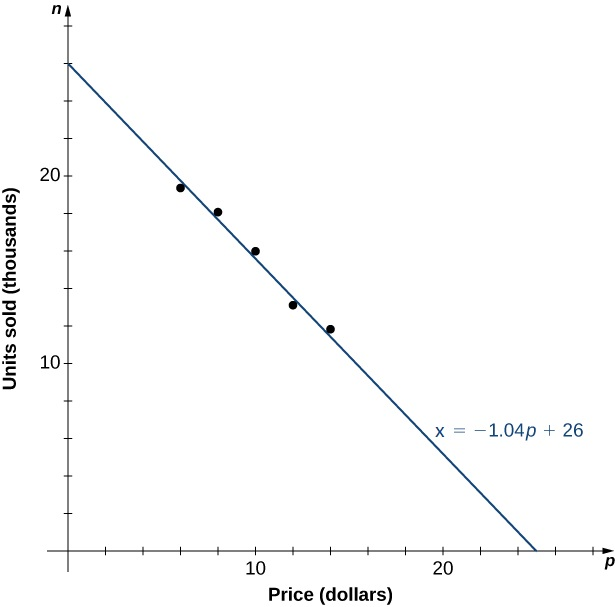
\includegraphics[width=\linewidth]{external/CNX_Calc_Figure_01_02_008x.jpg}
\end{image}%
\tcblower
\end{figureptx}%
\begin{example}{Maximizing Revenue.}{x:example:fs-id1170573569241}%
A company is interested in predicting the amount of revenue it will receive depending on the price it charges for a particular item. Using the data from \hyperref[x:table:fs-id1170573493744]{Table~{\xreffont\ref{x:table:fs-id1170573493744}}}, the company arrives at the following quadratic function to model revenue \(R\) (in thousands of dollars) as a function of price per item \(p:\)%
%
\begin{equation*}
R(p)=p\cdot( -1.04 p+ 26 )= -1.04p^2+ 26 p
\end{equation*}
for \(0 \leq  p\leq   25 .\)%
%
\begin{enumerate}
\item{}Predict the revenue if the company sells the item at a price of \(p=\$ 5 \) and \(p=\$ 17 .\)%
\item{}Find the zeros of this function and interpret the meaning of the zeros.%
\item{}Sketch a graph of \(R.\)%
\item{}Use the graph to determine the value of \(p\) that maximizes revenue. Find the maximum revenue.%
\end{enumerate}
\par\smallskip%
\noindent\textbf{\blocktitlefont Solution}.\hypertarget{g:solution:idm1621571176}{}\quad{}%
\begin{enumerate}
\item{}Evaluating the revenue function at \(p= 5 \) and \(p= 17 ,\) we can conclude that%
\begin{gather*}
R( 5 )= -1.04 ( 5 )^2+ 26 ( 5 )= 104 , \text{ so revenue } = \$104,000; \\
R( 17 )= -1.04( 17 )^2+ 26 ( 17 )= 141.44 , \text{ so revenue } =\$144,440.
\end{gather*}
%
\item{}The zeros of this function can be found by solving the equation \(-1.04p^2+ 26 p= 0 .\) When we factor the quadratic expression, we get \(p( -1.04 p+ 26 )= 0 .\) The solutions to this equation are given by \(p= 0 , 25 .\) For these values of \(p,\) the revenue is zero. When \(p=\$ 0 ,\) the revenue is zero because the company is giving away its merchandise for free. When \(p=\$ 25 ,\) the revenue is zero because the price is too high, and no one will buy any items.%
\item{}Knowing the fact that the function is quadratic, we also know the graph is a parabola. Since the leading coefficient is negative, the parabola opens downward. \begin{image}{0.25}{0.5}{0.25}%
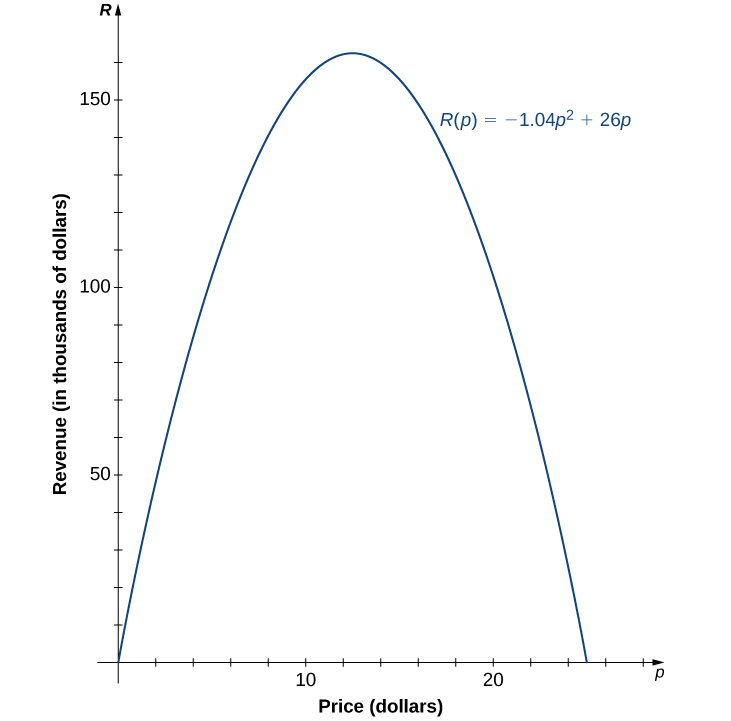
\includegraphics[width=\linewidth]{external/CNX_Calc_Figure_01_02_009.jpg}
\end{image}%
%
\item{}The function is a parabola opening downward. This means that its vertex point is a maximum. Using the vertex formula:%
\begin{equation*}
h=\frac{-b}{2a}=\frac{-26}{2(-1.04)}=12.5.
\end{equation*}
The maximum revenue occurs at a price of \(p=\$ 12.50 \) per item. At that price, the revenue is \(R(p)= -1.04 ( 12.5 )^2 + 26 ( 12.5 )=\$ 162 , 500 .\)%
\end{enumerate}
\end{example}
Recall that both the supply and demand equations \(p(x)\) give the price per unit given the number of units sold. This means that using either the supply or demand equation and that \(R=p\cdot x,\) we can find the revenue equation:%
\begin{equation*}
R=(\text{supply or demand equation})\cdot x.
\end{equation*}
%
\begin{example}{Maximizing Profit and Minimizing Cost.}{g:example:idm1621563752}%
A clothing store determines that its supply equation for \(x\) dresses sold is \(p=140-0.25x\) and the cost for producing \(x\) dresses is \(C(x)=2000-10x+0.25x^2\).%
%
\begin{enumerate}
\item{}Find the revenue function \(R(x)\).%
\item{}Find the profit function \(P(x)\).%
\item{}How many dresses must be sold in order to maximize profits?%
\item{}What is the maximum profit?%
\item{}How many dresses must be sold in order to minimize costs?%
\end{enumerate}
\par\smallskip%
\noindent\textbf{\blocktitlefont Solution}.\hypertarget{g:solution:idm1621559400}{}\quad{}%
\begin{enumerate}
\item{}We can find the revenue equation using the supply equation.%
\begin{equation*}
R(x)=p\cdot x
\end{equation*}
%
\begin{equation*}
R(x)=(140-0.25x)x
\end{equation*}
%
\begin{equation*}
R(x)=140x-0.25x^2\text{.}
\end{equation*}
%
\item{}Recall,%
\begin{equation*}
P=R-C
\end{equation*}
%
\begin{equation*}
P(x)=140x-0.25x^2-(2000-10x+0.25x^2)
\end{equation*}
%
\begin{equation*}
P(x)=-0.5x^2+150x-2000\text{.}
\end{equation*}
%
\item{}Since the profit function is a parabola opening downward, then the vertex of the profit function is a maximum.%
\begin{equation*}
h=\frac{-b}{2a}=\frac{-150}{2(-0.5)}=150
\end{equation*}
The clothing store must sell 150 dresses in order to maximize profits.%
\item{}Since selling 150 dresses maximizes profits, evaluating \(P(150)\) will give us the maximum profits. \(P(150)=-0.5(150)^2+150(150)-2000=\$ 9,250\) is the maximum profit.%
\item{}Observe that the cost equation \(C(x)=2000-10x+0.25x^2\) is a parabola opening upward. That is, its vertex is a minimum.%
\begin{equation*}
h=\frac{-b}{2a}=\frac{10}{2(0.25)}=20
\end{equation*}
The clothing store must sell 20 dresses in order to minimize costs.%
\end{enumerate}
\end{example}
\begin{inlineexercise}{}{g:exercise:idm1621552360}%
The demand equation for diamond rings sold at a jewelry store in one month is \(p=-0.05x+10.2\) where \(x\) is the number of diamond rings sold in one month and the price of each diamond ring is in thousands of dollars.%
%
\begin{enumerate}
\item{}Find the revenue function \(R(x)\).%
\item{}How many diamond rings must be sold in order to maximize revenue?%
\item{}What is the maximum revenue?%
\item{}What is the price per diamond ring that will maximize revenue?%
\end{enumerate}
\par\smallskip%
\noindent\textbf{\blocktitlefont Hint}.\hypertarget{g:hint:idm1621550184}{}\quad{}Use \(R=p\cdot x\) and the vertex of a parabola opening downward to find when revenue is maximized.\par\smallskip%
\noindent\textbf{\blocktitlefont Solution}.\hypertarget{g:solution:idm1621548264}{}\quad{}%
\begin{enumerate}
\item{}Using \(R=p\cdot x\) we obtain%
\begin{equation*}
R(x)=(-0.05x+10.2)\cdot x=-0.05x^2+10.2x.
\end{equation*}
%
\item{}Since the graph of our revenue function \(R(x)=-0.05x^2+10.2x\) opens downward, the vertex point will give us maximum revenue. Using the vertex formula,%
\begin{equation*}
h=-\frac{b}{2a}=-\frac{-10.2}{2(-0.05)}=102.
\end{equation*}
Furthermore, selling 102 diamond rings in one month will maximize revenue.%
\item{}Since revenue is maximized when 102 diamond rings are sold, evaluating \(R(102)\) will give us the maximum revenue.%
\begin{equation*}
R(102)=-0.05(102)^2+10.2(102)=520.2
\end{equation*}
Recalling that the price is in thousands of dollars, revenue will also be in thousands of dollars. As a result, the maximum revenue is \(520.2\cdot(\$ 1,000)=\$ 520,200\).%
\item{}In order to find the price per diamond ring that will maximize revenue we must evaluate the demand equation at \(x=102\).%
\begin{equation*}
p(102)=-0.05(102)+10.2=5.1
\end{equation*}
Again, since the price is in thousands of dollars, the price per diamond ring that will maximize revenue is \(5.1\cdot(\$1,000)=\$5,100\).%
\end{enumerate}
\end{inlineexercise}%
\end{subsectionptx}
This book is a custom edition based on OpenStax Calculus Volume 1. You can download the original for free at https:\slash{}\slash{}openstax.org\slash{}details\slash{}books\slash{}calculus-volume-1.%
\end{sectionptx}
%
%
\typeout{************************************************}
\typeout{Section 1.4 Inverse Functions}
\typeout{************************************************}
%
\begin{sectionptx}{Inverse Functions}{}{Inverse Functions}{}{}{x:section:suc_Ch1Sec4}
\begin{introduction}{Learning Objectives.}%
%
\begin{enumerate}
\item{}Determine the conditions for when a function has an inverse.%
\item{}Use the horizontal line test to recognize when a function is one-to-one.%
\item{}Find the inverse of a given function.%
\item{}Draw the graph of an inverse function.%
\item{}Evaluate inverse trigonometric functions.%
\end{enumerate}
An inverse function reverses the operation done by a particular function. In other words, whatever a function does, the inverse function undoes it. In this section, we define an inverse function formally and state the necessary conditions for an inverse function to exist. We examine how to find an inverse function and study the relationship between the graph of a function and the graph of its inverse. Then we apply these ideas to define and discuss properties of the inverse trigonometric functions.%
\end{introduction}%
%
%
\typeout{************************************************}
\typeout{Subsection 1.4.1 Existence of an Inverse Function}
\typeout{************************************************}
%
\begin{subsectionptx}{Existence of an Inverse Function}{}{Existence of an Inverse Function}{}{}{g:subsection:idm1621537256}
We begin with an example. Given a function \(f\) and an output \(y=f(x),\) we are often interested in finding what value or values \(x\) were mapped to \(y\) by \(f.\) For example, consider the function \(f(x)=x^3+4.\) Since any output \(y=x^3+4,\) we can solve this equation for \(x\) to find that the input is \(x=\sqrt[3]{y-3}.\) This equation defines \(x\) as a function of \(y.\) Denoting this function as \(f^{-1}\), and writing \(x=f^{-1} (y)=\sqrt[3]{y-3},\) we see that for any \(x\) in the domain of \(f,f^{-1} (f(x))=f^{-1} (x^3+4)=x.\) Thus, this new function, \(f^{-1} ,\) “undid” what the original function \(f\) did. A function with this property is called the inverse function of the original function.%
\begin{definition}{}{g:definition:idm1621528424}%
Given a function \(f\) with domain \(D\) and range \(R,\) its \terminology{inverse function} (if it exists) is the function \(f^{-1} \) with domain \(R\) and range \(D\) such that \(f^{-1} (y)=x\) if \(f(x)=y.\) In other words, for a function \(f\) and its inverse \(f^{-1} ,\)%
%
\begin{equation*}
f^{-1} (f(x))=x \text{ for all } x \text{ in } D,\text{ and } f(f^{-1} (y))=y \text{ for all } y \text{ in } R.
\end{equation*}
\end{definition}
Note that \(f^{-1} \) is read as “f inverse.” Here, the \(-1\) is not used as an exponent and \(f^{-1} (x)\neq 1/f(x).\) \hyperref[x:figure:CNX_Calc_Figure_01_04_001]{Figure~{\xreffont\ref{x:figure:CNX_Calc_Figure_01_04_001}}} shows the relationship between the domain and range of \(f\) and the domain and range of \(f^{-1} .\)%
\begin{figureptx}{Given a function \(f\) and its inverse \(f^{-1} ,f^{-1} (y)=x\) if and only if \(f(x)=y.\) The range of \(f\) becomes the domain of \(f^{-1} \) and the domain of \(f\) becomes the range of \(f^{-1} .\)}{x:figure:CNX_Calc_Figure_01_04_001}{}%
\begin{image}{0.25}{0.5}{0.25}%
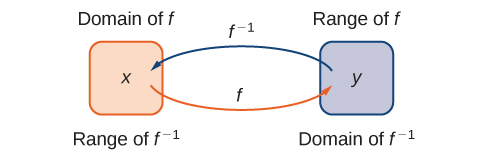
\includegraphics[width=\linewidth]{external/CNX_Calc_Figure_01_04_001.jpg}
\end{image}%
\tcblower
\end{figureptx}%
Recall that a function has exactly one output for each input. Therefore, to define an inverse function, we need to map each input to exactly one output. For example, let’s try to find the inverse function for \(f(x)=x^2.\) Solving the equation \(y=x^2\) for \(x,\) we arrive at the equation \(x=\pm \sqrt{y}.\) This equation does not describe \(x\) as a function of \(y\) because there are two solutions to this equation for every \(y\gt 0.\) The problem with trying to find an inverse function for \(f(x)=x^2\) is that two inputs are sent to the same output for each output \(y\gt 0.\) The function \(f(x)=x^3+4\) discussed earlier did not have this problem. For that function, each input was sent to a different output. A function that sends each input to a different output is called a one-to-one function.%
\begin{definition}{}{g:definition:idm1621513192}%
We say a \(f\) is a \terminology{one-to-one function} if \(f(x_1)\neq f(x_2)\) when \(x_1\neq x_2.\)%
\end{definition}
One way to determine whether a function is one-to-one is by looking at its graph. If a function is one-to-one, then no two inputs can be sent to the same output. Therefore, if we draw a horizontal line anywhere in the \(xy\)-plane, according to the \terminology{horizontal line test}, it cannot intersect the graph more than once. We note that the horizontal line test is different from the vertical line test. The vertical line test determines whether a graph is the graph of a function. The horizontal line test determines whether a function is one-to-one (\hyperref[x:figure:CNX_Calc_Figure_01_04_002]{Figure~{\xreffont\ref{x:figure:CNX_Calc_Figure_01_04_002}}}).%
\begin{note}{Rule: Horizontal Line Test.}{g:note:idm1621508968}%
A function \(f\) is one-to-one if and only if every horizontal line intersects the graph of \(f\) no more than once.%
\end{note}
\begin{figureptx}{(a) The function \(f(x)=x^2\) is not one-to-one because it fails the horizontal line test. (b) The function \(f(x)=x^3\) is one-to-one because it passes the horizontal line test.}{x:figure:CNX_Calc_Figure_01_04_002}{}%
\begin{image}{0.25}{0.5}{0.25}%
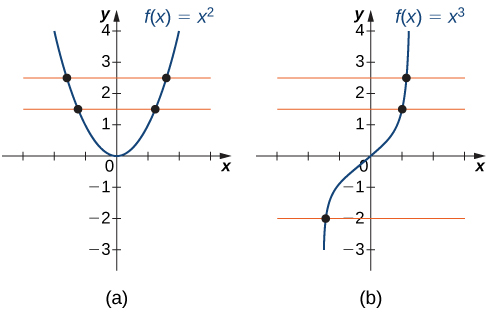
\includegraphics[width=\linewidth]{external/CNX_Calc_Figure_01_04_002.jpg}
\end{image}%
\tcblower
\end{figureptx}%
\begin{example}{Determining Whether a Function Is One-to-One.}{g:example:idm1621504232}%
For each of the following functions, use the horizontal line test to determine whether it is one-to-one.%
%
\begin{enumerate}
\item{}\begin{image}{0.25}{0.5}{0.25}%
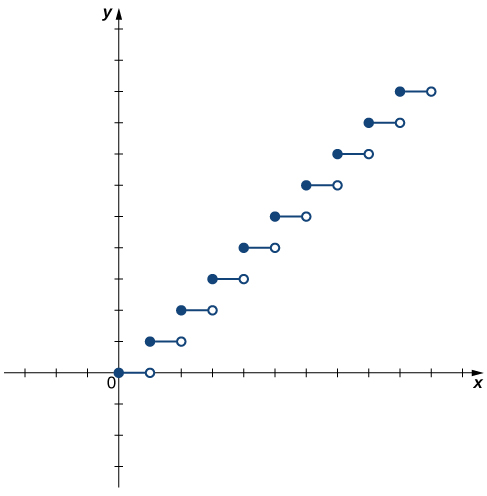
\includegraphics[width=\linewidth]{external/CNX_Calc_Figure_01_04_003.jpg}
\end{image}%
%
\item{}\begin{image}{0.25}{0.5}{0.25}%
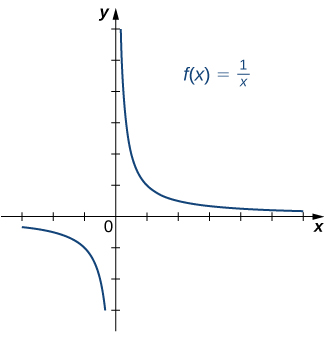
\includegraphics[width=\linewidth]{external/CNX_Calc_Figure_01_04_004.jpg}
\end{image}%
%
\end{enumerate}
\par\smallskip%
\noindent\textbf{\blocktitlefont Solution}.\hypertarget{g:solution:idm1621505512}{}\quad{}%
\begin{enumerate}
\item{}Since the horizontal line \(y=n\) for any integer \(n\geq 0\) intersects the graph more than once, this function is not one-to-one. \begin{image}{0.25}{0.5}{0.25}%
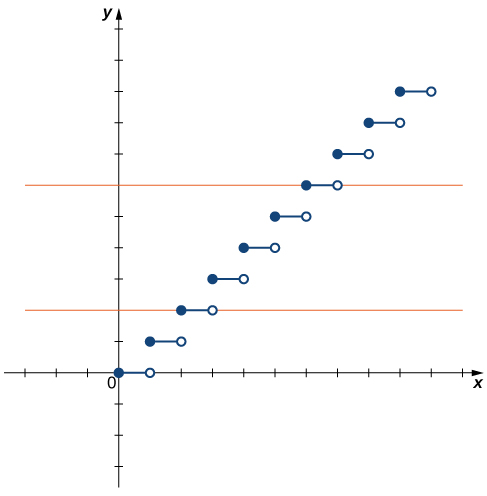
\includegraphics[width=\linewidth]{external/CNX_Calc_Figure_01_04_005.jpg}
\end{image}%
%
\item{}Since every horizontal line intersects the graph once (at most), this function is one-to-one. \begin{image}{0.25}{0.5}{0.25}%
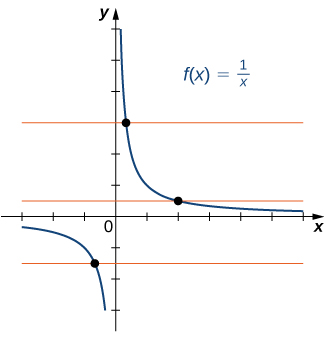
\includegraphics[width=\linewidth]{external/CNX_Calc_Figure_01_04_006.jpg}
\end{image}%
%
\end{enumerate}
\end{example}
\begin{inlineexercise}{}{g:exercise:idm1621498600}%
Is the function \(f\) graphed in the following image one-to-one?%
\begin{image}{0.25}{0.5}{0.25}%
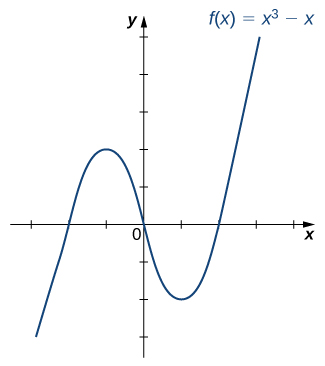
\includegraphics[width=\linewidth]{external/CNX_Calc_Figure_01_04_007.jpg}
\end{image}%
\par\smallskip%
\noindent\textbf{\blocktitlefont Hint}.\hypertarget{g:hint:idm1621497448}{}\quad{}Use the horizontal line test.%
\par\smallskip%
\noindent\textbf{\blocktitlefont Solution}.\hypertarget{g:solution:idm1621498216}{}\quad{}No.%
\end{inlineexercise}%
\end{subsectionptx}
%
%
\typeout{************************************************}
\typeout{Subsection 1.4.2 Finding a Function’s Inverse}
\typeout{************************************************}
%
\begin{subsectionptx}{Finding a Function’s Inverse}{}{Finding a Function’s Inverse}{}{}{g:subsection:idm1621497320}
We can now consider one-to-one functions and show how to find their inverses. Recall that a function maps elements in the domain of \(f\) to elements in the range of \(f.\) The inverse function maps each element from the range of \(f\) back to its corresponding element from the domain of \(f.\) Therefore, to find the inverse function of a one-to-one function \(f,\) given any \(y\) in the range of \(f,\) we need to determine which \(x\) in the domain of \(f\) satisfies \(f(x)=y.\) Since \(f\) is one-to-one, there is exactly one such value \(x.\) We can find that value \(x\) by solving the equation \(f(x)=y\) for \(x.\) Doing so, we are able to write \(x\) as a function of \(y\) where the domain of this function is the range of \(f\) and the range of this new function is the domain of \(f.\) Consequently, this function is the inverse of \(f,\) and we write \(x=f^{-1} (y).\) Since we typically use the variable \(x\) to denote the independent variable and \(y\) to denote the dependent variable, we often interchange the roles of \(x\) and \(y,\) and write \(y=f^{-1} (x).\) Representing the inverse function in this way is also helpful later when we graph a function \(f\) and its inverse \(f^{-1} \) on the same axes.%
\begin{note}{Problem-Solving Strategy: Finding an Inverse Function.}{x:note:fs-id1170572552427}%
%
\begin{enumerate}
\item{}Solve the equation \(y=f(x)\) for \(x.\)%
\item{}Interchange the variables \(x\) and \(y\) and write \(y=f^{-1} (x).\)%
\end{enumerate}
\end{note}
\begin{example}{Finding an Inverse Function.}{g:example:idm1621481192}%
Find the inverse for the function \(f(x)=3x-4.\) State the domain and range of the inverse function. Verify that \(f^{-1} (f(x))=x.\)%
\par\smallskip%
\noindent\textbf{\blocktitlefont Solution}.\hypertarget{g:solution:idm1621478760}{}\quad{}Follow the steps outlined in the strategy.%
\par
Step 1. If \(y=3x-4,\) then \(3x=y+4\) and \(x= \frac{1}{3}y+ \frac{4}{3}.\)%
\par
Step 2. Rewrite as \(y=\frac{1}{3}x+ \frac{4}{3}\) and let \(y=f^{-1} (x).\)%
\par
Therefore, \(f^{-1} (x)= \frac{1}{3}x+ \frac{4}{3}.\)%
\par
Since the domain of \(f\) is \((-\infty ,\infty ),\) the range of \(f^{-1} \) is \((-\infty ,\infty ).\) Since the range of \(f\) is \((-\infty ,\infty ),\) the domain of \(f^{-1} \) is \((-\infty ,\infty ).\)%
\par
You can verify that \(f^{-1} (f(x))=x\) by writing%
%
\begin{equation*}
f^{-1} (f(x))=f^{-1} (3x-4)= \frac{1}{3}(3x-4)+ \frac{4}{3}=x- \frac{4}{3}+ \frac{4}{3}=x.
\end{equation*}
Note that for \(f^{-1} (x)\) to be the inverse of \(f(x),\) both \(f^{-1} (f(x))=x\) and \(f(f^{-1} (x))=x\) for all \(x\) in the domain of the inside function.%
\end{example}
\begin{inlineexercise}{}{g:exercise:idm1621468904}%
Find the inverse of the function \(f(x)=3x/(x-2).\) State the domain and range of the inverse function.%
\par\smallskip%
\noindent\textbf{\blocktitlefont Hint}.\hypertarget{g:hint:idm1621468008}{}\quad{}Use the \hyperref[x:note:fs-id1170572552427]{Note~{\xreffont\ref{x:note:fs-id1170572552427}}} for finding inverse functions.%
\par\smallskip%
\noindent\textbf{\blocktitlefont Solution}.\hypertarget{g:solution:idm1621467624}{}\quad{}\(f^{-1} (x)= \frac{2x}{x-3}.\) The domain of \(f^{-1} \) is \(\{x|x\neq 3\}.\) The range of \(f^{-1} \) is \(\{y|y\neq 2\}.\)%
\end{inlineexercise}%
%
%
\typeout{************************************************}
\typeout{Subsubsection 1.4.2.1 Graphing Inverse Functions}
\typeout{************************************************}
%
\begin{subsubsectionptx}{Graphing Inverse Functions}{}{Graphing Inverse Functions}{}{}{g:subsubsection:idm1621463784}
Let’s consider the relationship between the graph of a function \(f\) and the graph of its inverse. Consider the graph of \(f\) shown in \hyperref[x:figure:CNX_Calc_Figure_01_04_008]{Figure~{\xreffont\ref{x:figure:CNX_Calc_Figure_01_04_008}}} and a point \((a,b)\) on the graph. Since \(b=f(a),\) then \(f^{-1} (b)=a.\) Therefore, when we graph \(f^{-1} ,\) the point \((b,a)\) is on the graph. As a result, the graph of \(f^{-1} \) is a reflection of the graph of \(f\) about the line \(y=x.\)%
\begin{figureptx}{(a) The graph of this function \(f\) shows point \((a,b)\) on the graph of \(f.\) (b) Since \((a,b)\) is on the graph of \(f,\) the point \((b,a)\) is on the graph of \(f^{-1} .\) The graph of \(f^{-1} \) is a reflection of the graph of \(f\) about the line \(y=x.\)}{x:figure:CNX_Calc_Figure_01_04_008}{}%
\begin{image}{0.25}{0.5}{0.25}%
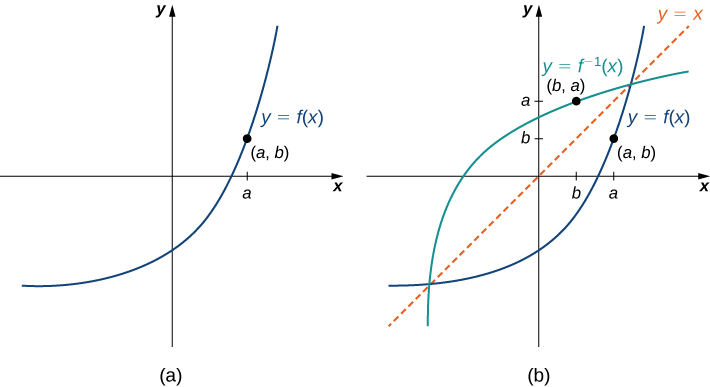
\includegraphics[width=\linewidth]{external/CNX_Calc_Figure_01_04_017.jpg}
\end{image}%
\tcblower
\end{figureptx}%
\begin{example}{Sketching Graphs of Inverse Functions.}{g:example:idm1621447016}%
For the graph of \(f\) in the following image, sketch a graph of \(f^{-1} \) by sketching the line \(y=x\) and using symmetry. Identify the domain and range of \(f^{-1} .\)%
\begin{image}{0.25}{0.5}{0.25}%
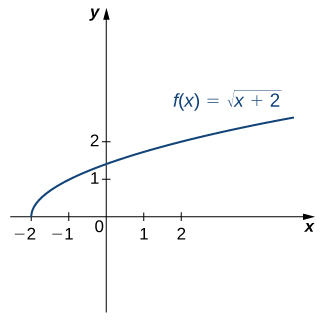
\includegraphics[width=\linewidth]{external/CNX_Calc_Figure_01_04_009.jpg}
\end{image}%
\par\smallskip%
\noindent\textbf{\blocktitlefont Solution}.\hypertarget{g:solution:idm1621448296}{}\quad{}Reflect the graph about the line \(y=x.\) The domain of \(f^{-1} \) is \([0,\infty ).\) The range of \(f^{-1} \) is \([-2,\infty ).\) By using the preceding strategy for finding inverse functions, we can verify that the inverse function is \(f^{-1} (x)=x^2-2,\) as shown in the graph.%
\begin{image}{0.25}{0.5}{0.25}%
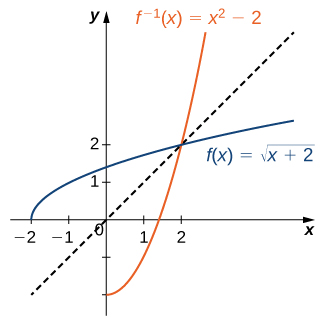
\includegraphics[width=\linewidth]{external/CNX_Calc_Figure_01_04_010.jpg}
\end{image}%
\end{example}
\begin{inlineexercise}{}{g:exercise:idm1621441640}%
Sketch the graph of \(f(x)=2x+3\) and the graph of its inverse using the symmetry property of inverse functions.%
\par\smallskip%
\noindent\textbf{\blocktitlefont Hint}.\hypertarget{g:hint:idm1621438568}{}\quad{}The graphs are symmetric about the line \(y=x.\)%
\par\smallskip%
\noindent\textbf{\blocktitlefont Solution}.\hypertarget{g:solution:idm1621440616}{}\quad{} \begin{image}{0.25}{0.5}{0.25}%
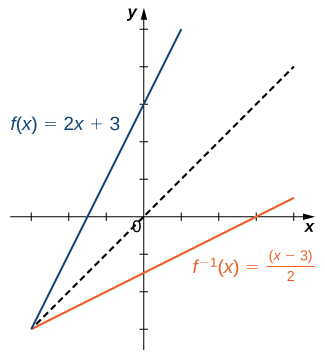
\includegraphics[width=\linewidth]{external/CNX_Calc_Figure_01_04_011.jpg}
\end{image}%
%
\end{inlineexercise}%
\end{subsubsectionptx}
%
%
\typeout{************************************************}
\typeout{Subsubsection 1.4.2.2 Restricting Domains}
\typeout{************************************************}
%
\begin{subsubsectionptx}{Restricting Domains}{}{Restricting Domains}{}{}{g:subsubsection:idm1621437416}
As we have seen, \(f(x)=x^2\) does not have an inverse function because it is not one-to-one. However, we can choose a subset of the domain of \(f\) such that the function is one-to-one. This subset is called a \terminology{restricted domain}. By restricting the domain of \(f,\) we can define a new function \(g\) such that the domain of \(g\) is the restricted domain of \(f\) and \(g(x)=f(x)\) for all \(x\) in the domain of \(g.\) Then we can define an inverse function for \(g\) on that domain. For example, since \(f(x)=x^2\) is one-to-one on the interval \([0,\infty ),\) we can define a new function \(g\) such that the domain of \(g\) is \([0,\infty )\) and \(g(x)=x^2\) for all \(x\) in its domain. Since \(g\) is a one-to-one function, it has an inverse function, given by the formula \(g^{-1}(x)=\sqrt{x}.\) On the other hand, the function \(f(x)=x^2\) is also one-to-one on the domain \((-\infty ,0].\) Therefore, we could also define a new function \(h\) such that the domain of \(h\) is \((-\infty ,0]\) and \(h(x)=x^2\) for all \(x\) in the domain of \(h.\) Then \(h\) is a one-to-one function and must also have an inverse. Its inverse is given by the formula \(h^{-1}(x)=-\sqrt{x}\) (\hyperref[x:figure:CNX_Calc_Figure_01_04_012]{Figure~{\xreffont\ref{x:figure:CNX_Calc_Figure_01_04_012}}}).%
\begin{figureptx}{(a) For \(g(x)=x^2\) restricted to \([0,\infty ),g^{-1}(x)=\sqrt{x}.\) (b) For \(h(x)=x^2\) restricted to \((-\infty ,0],h^{-1}(x)=-\sqrt{x}.\)}{x:figure:CNX_Calc_Figure_01_04_012}{}%
\begin{image}{0.25}{0.5}{0.25}%
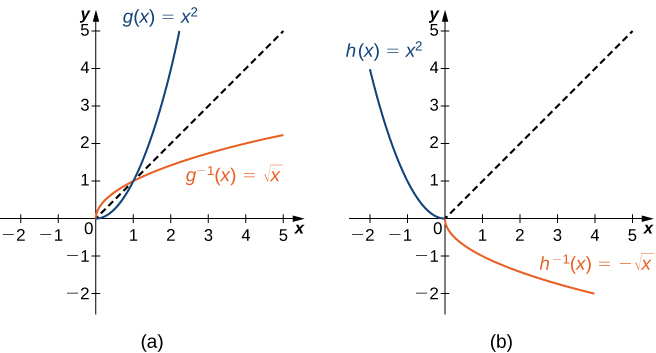
\includegraphics[width=\linewidth]{external/CNX_Calc_Figure_01_04_012.jpg}
\end{image}%
\tcblower
\end{figureptx}%
\begin{example}{Restricting the Domain.}{g:example:idm1621421288}%
Consider the function \(f(x)=(x+1)^2.\)%
%
\begin{enumerate}
\item{}Sketch the graph of \(f\) and use the horizontal line test to show that \(f\) is not one-to-one.%
\item{}Show that \(f\) is one-to-one on the restricted domain \([-1,\infty ).\) Determine the domain and range for the inverse of \(f\) on this restricted domain and find a formula for \(f^{-1} .\)%
\end{enumerate}
\par\smallskip%
\noindent\textbf{\blocktitlefont Solution}.\hypertarget{g:solution:idm1621420008}{}\quad{}%
\begin{enumerate}
\item{}The graph of \(f\) is the graph of \(y=x^2\) shifted left 1 unit. Since there exists a horizontal line intersecting the graph more than once, \(f\) is not one-to-one. \begin{image}{0.25}{0.5}{0.25}%
\includegraphics[width=\linewidth]{external/CNX_Calc_Figure_01_04_013.jpg}
\end{image}%
%
\item{}On the interval \([-1,\infty ), f\) is one-to-one. \begin{image}{0.25}{0.5}{0.25}%
\includegraphics[width=\linewidth]{external/CNX_Calc_Figure_01_04_014.jpg}
\end{image}%
  The domain and range of \(f^{-1} \) are given by the range and domain of \(f,\) respectively. Therefore, the domain of \(f^{-1} \) is \([0,\infty )\) and the range of \(f^{-1} \) is \([-1,\infty ).\) To find a formula for \(f^{-1} ,\) solve the equation \(y=(x+1)^2\) for \(x.\) If \(y=(x+1)^2,\) then \(x=-1\pm \sqrt{y}.\) Since we are restricting the domain to the interval where \(x\geq -1,\) we need \(\pm \sqrt{y}\geq 0.\) Therefore, \(x=-1+\sqrt{y}.\) Interchanging \(x\) and \(y,\) we write \(y=-1+\sqrt{x}\) and conclude that \(f^{-1} (x)=-1+\sqrt{x}.\)%
\end{enumerate}
\end{example}
\begin{inlineexercise}{}{g:exercise:idm1621408104}%
Consider \(f(x)=1/x^2\) restricted to the domain \((-\infty ,0).\) Verify that \(f\) is one-to-one on this domain. Determine the domain and range of the inverse of \(f\) and find a formula for \(f^{-1} .\)%
\par\smallskip%
\noindent\textbf{\blocktitlefont Hint}.\hypertarget{g:hint:idm1621404136}{}\quad{}The domain and range of \(f^{-1} \) is given by the range and domain of \(f,\) respectively. To find \(f^{-1} ,\) solve \(y=1/x^2\) for \(x.\)%
\par\smallskip%
\noindent\textbf{\blocktitlefont Solution}.\hypertarget{g:solution:idm1621401064}{}\quad{}The domain of \(f^{-1} \) is \((0,\infty ).\) The range of \(f^{-1} \) is \((-\infty ,0).\) The inverse function is given by the formula \(f^{-1} (x)=-1/\sqrt{x}.\)%
\end{inlineexercise}%
\end{subsubsectionptx}
\end{subsectionptx}
%
%
\typeout{************************************************}
\typeout{Subsection 1.4.3 Inverse Trigonometric Functions}
\typeout{************************************************}
%
\begin{subsectionptx}{Inverse Trigonometric Functions}{}{Inverse Trigonometric Functions}{}{}{g:subsection:idm1621397224}
The six basic trigonometric functions are periodic, and therefore they are not one-to-one. However, if we restrict the domain of a trigonometric function to an interval where it is one-to-one, we can define its inverse. Consider the sine function. The sine function is one-to-one on an infinite number of intervals, but the standard convention is to restrict the domain to the interval \([- \frac{\pi}{2},\frac{\pi}{2}].\) By doing so, we define the inverse sine function on the domain \([-1,1]\) such that for any \(x\) in the interval \([-1,1],\) the inverse sine function tells us which angle \(\theta \) in the interval \([-\frac{\pi}{2},\frac{\pi}{2}]\) satisfies \(\sin\,\theta =x.\) Similarly, we can restrict the domains of the other trigonometric functions to define \terminology{inverse trigonometric functions}, which are functions that tell us which angle in a certain interval has a specified trigonometric value.%
\begin{definition}{}{g:definition:idm1621393512}%
The inverse sine function, denoted \(\sin^{-1} \) or arcsin, and the inverse cosine function, denoted \(\cos^{-1}\) or arccos, are defined on the domain \(D=\{x|-1\leq  x\leq  1\}\) as follows:%
%
\begin{align*}
\sin^{-1} (x) \amp =y \text{ if and only if } \sin(y)=x \text{ and } -\frac{\pi}{2}\leq  y\leq  \frac{\pi}{2} \\
\cos^{-1}(x)\amp =y \text{ if and only if } \text{ cos }(y)=x \text{ and } 0\leq  y\leq  \pi. 
\end{align*}
The inverse tangent function, denoted \(\tan^{-1} \) or arctan, and inverse cotangent function, denoted \(\cot^{-1} \) or arccot, are defined on the domain \(D=\{x|-\infty \lt x\lt \infty \}\) as follows:%
%
\begin{gather*}
\tan^{-1} (x)=y \text{ if and only if } \text{ tan }(y)=x \text{ and } -\frac{\pi}{2}\lt y\lt \frac{\pi}{2};\\
\cot^{-1} (x)=y \text{ if and only if } \text{ cot }(y)=x \text{ and } 0\lt y\lt \pi.
\end{gather*}
The inverse cosecant function, denoted \(\csc^{-1} \) or arccsc, and inverse secant function, denoted \(\sec^{-1} \) or arcsec, are defined on the domain \(D=\{x||x|\geq \}\) as follows:%
%
\begin{gather*}
\csc^{-1} (x)=y \text{ if and only if } \text{ csc }(y)=x \text{ and } -\frac{\pi}{2}\leq  y\leq  \frac{\pi}{2},y\neq 0;\\
\sec^{-1} (x)=y \text{ if and only if } \text{ sec }(y)=x \text{ and } 0\leq  y\leq  \pi,y\neq \pi/2.
\end{gather*}
\end{definition}
To graph the inverse trigonometric functions, we use the graphs of the trigonometric functions restricted to the domains defined earlier and reflect the graphs about the line \(y=x\) (\hyperref[x:figure:CNX_Calc_Figure_01_04_015]{Figure~{\xreffont\ref{x:figure:CNX_Calc_Figure_01_04_015}}}).%
\begin{figureptx}{The graph of each of the inverse trigonometric functions is a reflection about the line \(y=x\) of the corresponding restricted trigonometric function.}{x:figure:CNX_Calc_Figure_01_04_015}{}%
\begin{image}{0.25}{0.5}{0.25}%
\includegraphics[width=\linewidth]{external/CNX_Calc_Figure_01_04_018.jpg}
\end{image}%
\tcblower
\end{figureptx}%
\begin{note}{}{g:note:idm1621386344}%
Go to the following site for more comparisons of functions and their inverses.%
\end{note}
When evaluating an inverse trigonometric function, the output is an angle. For example, to evaluate \(\cos^{-1}(\frac{1}{2}),\) we need to find an angle \(\theta \) such that \(\text{ cos }\,\theta =\frac{1}{2}.\) Clearly, many angles have this property. However, given the definition of \(\cos^{-1},\) we need the angle \(\theta \) that not only solves this equation, but also lies in the interval \([0,\pi].\) We conclude that \(\cos^{-1}(\frac{1}{2})=\frac{\pi}{3}.\)%
\par
We now consider a composition of a trigonometric function and its inverse. For example, consider the two expressions \(\sin(\sin^{-1} (\frac{\sqrt{2}}{2}))\) and \(\sin^{-1} (\sin(\pi)).\) For the first one, we simplify as follows:%
%
\begin{equation*}
\sin(\sin^{-1} ( \frac{\sqrt{2}}{2}))=\sin( \frac{\pi}{4})= \frac{\sqrt{2}}{2}.
\end{equation*}
For the second one, we have%
%
\begin{equation*}
\sin^{-1} (\sin(\pi))=\sin^{-1} (0)=0.
\end{equation*}
The inverse function is supposed to “undo” the original function, so why isn’t \(\sin^{-1} (\sin(\pi))=\pi?\) Recalling our definition of inverse functions, a function \(f\) and its inverse \(f^{-1} \) satisfy the conditions \(f(f^{-1} (y))=y\) for all \(y\) in the domain of \(f^{-1} \) and \(f^{-1} (f(x))=x\) for all \(x\) in the domain of \(f,\) so what happened here? The issue is that the inverse sine function, \(\sin^{-1} ,\) is the inverse of the restricted sine function defined on the domain \([-\frac{\pi}{2},\frac{\pi}{2}].\) Therefore, for \(x\) in the interval \([-\frac{\pi}{2},\frac{\pi}{2}]\text{ , }\) it is true that \(\sin^{-1} (\sin\,x)=x.\) However, for values of \(x\) outside this interval, the equation does not hold, even though \(\sin^{-1} (\sin\,x)\) is defined for all real numbers \(x.\)%
\par
What about \(\sin(\sin^{-1} y)?\) Does that have a similar issue? The answer is no. Since the domain of \(\sin^{-1} \) is the interval \([-1,1],\) we conclude that \(\sin(\sin^{-1} y)=y\) if \(-1\leq  y\leq  1\) and the expression is not defined for other values of \(y.\) To summarize,%
%
\begin{equation*}
\sin(\sin^{-1} y)=y \text{ if } -1\leq  y\leq  1
\end{equation*}
and%
%
\begin{equation*}
\sin^{-1} (\sin\,x)=x \text{ if } -\frac{\pi}{2}\leq  x\leq  \frac{\pi}{2}.
\end{equation*}
Similarly, for the cosine function,%
%
\begin{equation*}
\text{ cos }(\cos^{-1}y)=y \text{ if } -1\leq  y\leq  1
\end{equation*}
and%
%
\begin{equation*}
\cos^{-1}(\text{ cos }\,x)=x \text{ if } 0\leq  x\leq  \pi.
\end{equation*}
Similar properties hold for the other trigonometric functions and their inverses.%
\begin{example}{Evaluating Expressions Involving Inverse Trigonometric Functions.}{g:example:idm1621365992}%
Evaluate each of the following expressions.%
%
\begin{enumerate}
\item{}\(\displaystyle \sin^{-1} (- \frac{\sqrt{3}}{2})\)%
\item{}\(\displaystyle \text{ tan }(\tan^{-1} (- \frac{1}{\sqrt{3}}))\)%
\item{}\(\displaystyle \cos^{-1}(\text{ cos }( \frac{5\pi}{4}))\)%
\item{}\(\displaystyle \sin^{-1} (\text{ cos }( \frac{2\pi}{3}))\)%
\end{enumerate}
\par\smallskip%
\noindent\textbf{\blocktitlefont Solution}.\hypertarget{g:solution:idm1621360616}{}\quad{}%
\begin{enumerate}
\item{}Evaluating \(\sin^{-1} (-\sqrt{3}/2)\) is equivalent to finding the angle \(\theta \) such that \(\sin\,\theta =-\sqrt{3}/2\) and \(-\pi/2\leq  \theta \leq  \pi/2.\) The angle \(\theta =-\pi/3\) satisfies these two conditions. Therefore, \(\sin^{-1} (-\sqrt{3}/2)=-\pi/3.\)%
\item{}First we use the fact that \(\tan^{-1} (-1/\sqrt{3})=-\pi/6.\) Then \(\text{ tan }(\pi/6)=-1/\sqrt{3}.\) Therefore, \(\text{ tan }(\tan^{-1} (-1/\sqrt{3}))=-1/\sqrt{3}.\)%
\item{}To evaluate \(\cos^{-1}(\text{ cos }(5\pi/4)),\) first use the fact that \(\text{ cos }(5\pi/4)=-\sqrt{2}/2.\) Then we need to find the angle \(\theta \) such that \(\text{ cos }(\theta )=-\sqrt{2}/2\) and \(0\leq  \theta \leq  \pi.\) Since \(3\pi/4\) satisfies both these conditions, we have \(\text{ cos }(\cos^{-1}(5\pi/4))=\text{ cos }(\cos^{-1}(-\sqrt{2}/2))=3\pi/4.\)%
\item{}Since \(\text{ cos }(2\pi/3)=-1/2,\) we need to evaluate \(\sin^{-1} (-1/2).\) That is, we need to find the angle \(\theta \) such that \(\sin(\theta )=-1/2\) and \(-\pi/2\leq  \theta \leq  \pi/2.\) Since \(-\pi/6\) satisfies both these conditions, we can conclude that \(\sin^{-1} (\text{ cos }(2\pi/3))=\sin^{-1} (-1/2)=-\pi/6.\)%
\end{enumerate}
\end{example}
\begin{note}{Project: The Maximum Value of a Function.}{g:note:idm1621352296}%
In many areas of science, engineering, and mathematics, it is useful to know the maximum value a function can obtain, even if we don’t know its exact value at a given instant. For instance, if we have a function describing the strength of a roof beam, we would want to know the maximum weight the beam can support without breaking. If we have a function that describes the speed of a train, we would want to know its maximum speed before it jumps off the rails. Safe design often depends on knowing maximum values.%
\par
This project describes a simple example of a function with a maximum value that depends on two equation coefficients. We will see that maximum values can depend on several factors other than the independent variable \(x\).%
%
\begin{enumerate}
\item{}Consider the graph in \hyperref[x:figure:CNX_Calc_Figure_01_04_016]{Figure~{\xreffont\ref{x:figure:CNX_Calc_Figure_01_04_016}}} of the function \(y=\sin\,x+\text{ cos }\,x.\) Describe its overall shape. Is it periodic? How do you know? \begin{figureptx}{The graph of \(y=\sin\,x+\text{ cos }\,x.\)}{x:figure:CNX_Calc_Figure_01_04_016}{}%
\begin{image}{0.25}{0.5}{0.25}%
\includegraphics[width=\linewidth]{external/CNX_Calc_Figure_01_04_016.jpg}
\end{image}%
\tcblower
\end{figureptx}%
 Using a graphing calculator or other graphing device, estimate the \(x\)- and \(y\)-values of the maximum point for the graph (the first such point where \(x\) \textbackslash{}gt  0). It may be helpful to express the \(x\)-value as a multiple of \textbackslash{}pi.%
\item{}Now consider other graphs of the form \(y=A\,\sin\,x+B\,\text{ cos }\,x\) for various values of \(A\) and \(B\). Sketch the graph when \(A\) = 2 and \(B\) = 1, and find the \(x\)- and \(y\)-values for the maximum point. (Remember to express the \(x\)-value as a multiple of \textbackslash{}pi, if possible.) Has it moved?%
\item{}Repeat for \(A\) = 1, \(B\) = 2. Is there any relationship to what you found in part (2)?%
\item{}Complete the following table, adding a few choices of your own for \(A\) and \(B\): \begin{tableptx}{\textbf{}}{x:table:fs-id1170572554057}{}%
\centering%
{\tabularfont%
\begin{tabular}{lllllllll}
\textbf{\(A\)}&\textbf{\(B\)}&\textbf{\(x\)}&\textbf{\(y\)}&\textbf{}&\textbf{\(A\)}&\textbf{\(B\)}&\textbf{\(x\)}&\textbf{\(y\)}\tabularnewline\hrulethick
0&1&&&&\(\sqrt{3}\)&1&&\tabularnewline[0pt]
1&0&&&&1&\(\sqrt{3}\)&&\tabularnewline[0pt]
1&1&&&&12&5&&\tabularnewline[0pt]
1&2&&&&5&12&&\tabularnewline[0pt]
2&1&&&&&&&\tabularnewline[0pt]
2&2&&&&&&&\tabularnewline[0pt]
3&4&&&&&&&\tabularnewline[0pt]
4&3&&&&&&&
\end{tabular}
}%
\end{tableptx}%
%
\item{}Try to figure out the formula for the \(y\)-values.%
\item{}The formula for the \(x\)-values is a little harder. The most helpful points from the table are \((1,1),(1,\sqrt{3}),(\sqrt{3},1).\) (Hint: Consider inverse trigonometric functions.)%
\item{}If you found formulas for parts (5) and (6), show that they work together. That is, substitute the \(x\)-value formula you found into \(y=A\,\sin\,x+B\,\text{ cos }\,x\) and simplify it to arrive at the \(y\)-value formula you found.%
\end{enumerate}
\end{note}
\end{subsectionptx}
%
%
\typeout{************************************************}
\typeout{Subsection 1.4.4 Key Concepts}
\typeout{************************************************}
%
\begin{subsectionptx}{Key Concepts}{}{Key Concepts}{}{}{g:subsection:idm1621167080}
%
\begin{itemize}[label=\textbullet]
\item{}For a function to have an inverse, the function must be one-to-one. Given the graph of a function, we can determine whether the function is one-to-one by using the horizontal line test.%
\item{}If a function is not one-to-one, we can restrict the domain to a smaller domain where the function is one-to-one and then define the inverse of the function on the smaller domain.%
\item{}For a function \(f\) and its inverse \(f^{-1} ,f(f^{-1} (x))=x\) for all \(x\) in the domain of \(f^{-1} \) and \(f^{-1} (f(x))=x\) for all \(x\) in the domain of \(f.\)%
\item{}Since the trigonometric functions are periodic, we need to restrict their domains to define the inverse trigonometric functions.%
\item{}The graph of a function \(f\) and its inverse \(f^{-1} \) are symmetric about the line \(y=x.\)%
\end{itemize}
\end{subsectionptx}
%
%
\typeout{************************************************}
\typeout{Subsection 1.4.5 Key Equations}
\typeout{************************************************}
%
\begin{subsectionptx}{Key Equations}{}{Key Equations}{}{}{g:subsection:idm1621160680}
%
\begin{enumerate}
\item{}Inverse functions \(f^{-1} (f(x))=x \text{ for all } x \text{ in } D,\text{ and } f(f^{-1} (y))=y \text{ for all } y \text{ in } R.\)%
\end{enumerate}
\end{subsectionptx}
This book is a custom edition based on OpenStax Calculus Volume 1. You can download the original for free at https:\slash{}\slash{}openstax.org\slash{}details\slash{}books\slash{}calculus-volume-1.%
\end{sectionptx}
%
%
\typeout{************************************************}
\typeout{Section 1.5 Exponential and Logarithmic Functions}
\typeout{************************************************}
%
\begin{sectionptx}{Exponential and Logarithmic Functions}{}{Exponential and Logarithmic Functions}{}{}{x:section:sec_Ch1Sec5}
\begin{introduction}{Learning Objectives.}%
%
\begin{enumerate}
\item{}Identify the form of an exponential function.%
\item{}Explain the difference between the graphs of \(x^b\) and \(b^x.\)%
\item{}Recognize the significance of the number \(e.\)%
\item{}Identify the form of a logarithmic function.%
\item{}Explain the relationship between exponential and logarithmic functions.%
\item{}Describe how to calculate a logarithm to a different base.%
\end{enumerate}
In this section we examine exponential and logarithmic functions. We use the properties of these functions to solve equations involving exponential or logarithmic terms, and we study the meaning and importance of the number \(e.\) We also define hyperbolic and inverse hyperbolic functions, which involve combinations of exponential and logarithmic functions. (Note that we present alternative definitions of exponential and logarithmic functions in the chapter  Applications of Integrations , and prove that the functions have the same properties with either definition.)%
\end{introduction}%
%
%
\typeout{************************************************}
\typeout{Subsection 1.5.1 Exponential Functions}
\typeout{************************************************}
%
\begin{subsectionptx}{Exponential Functions}{}{Exponential Functions}{}{}{g:subsection:idm1621150568}
\begin{introduction}{}%
Exponential functions arise in many applications. One common example is \terminology{population growth}.%
\par
For example, if a population starts with \(P_0\) individuals and then grows at an annual rate of \(2\%,\) its population after 1 year is%
%
\begin{equation*}
P(1)=P_0+0.02P_0=P_0(1+0.02)=P_0(1.02).
\end{equation*}
Its population after 2 years is%
%
\begin{equation*}
P(2)=P(1)+0.02P(1)=P(1)(1.02)=P_0(1.02)^2.
\end{equation*}
In general, its population after \(t\) years is%
%
\begin{equation*}
P(t)=P_0(1.02)^t,
\end{equation*}
which is an exponential function. More generally, any function of the form \(f(x)=b^x,\) where \(b\gt 0,b\neq 1,\) is an exponential function with \terminology{base} \(b\) and \terminology{exponent} \(x\). Exponential functions have constant bases and variable exponents. Note that a function of the form \(f(x)=x^b\) for some constant \(b\) is not an exponential function but a power function.%
\par
To see the difference between an exponential function and a power function, we compare the functions \(y=x^2\) and \(y=2^x.\) In \hyperref[x:table:fs-id1170572205233]{Table~{\xreffont\ref{x:table:fs-id1170572205233}}}, we see that both \(2^x\) and \(x^2\) approach infinity as \(x\to \infty.\) Eventually, however, \(2^x\) becomes larger than \(x^2\) and grows more rapidly as \(x\to \infty.\) In the opposite direction, as \(x\to .\infty,x^2\to \infty,\) whereas \(2^x\to 0.\) The line \(y=0\) is a horizontal asymptote for \(y=2^x.\)%
\begin{tableptx}{\textbf{Values of \(x^2\) and \(2^x\)}}{x:table:fs-id1170572205233}{}%
\centering%
{\tabularfont%
\begin{tabular}{lllllllllll}
\multicolumn{1}{c}{\(x\)}&\multicolumn{1}{c}{\(-3\)}&\multicolumn{1}{c}{\(-2\)}&\multicolumn{1}{c}{\(-1\)}&\multicolumn{1}{c}{\(0\)}&\multicolumn{1}{c}{\(1\)}&\multicolumn{1}{c}{\(2\)}&\multicolumn{1}{c}{\(3\)}&\multicolumn{1}{c}{\(4\)}&\multicolumn{1}{c}{\(5\)}&\multicolumn{1}{c}{\(6\)}\tabularnewline[0pt]
\multicolumn{1}{c}{\(x^2\)}&\multicolumn{1}{c}{\(9\)}&\multicolumn{1}{c}{\(4\)}&\multicolumn{1}{c}{\(1\)}&\multicolumn{1}{c}{\(0\)}&\multicolumn{1}{c}{\(1\)}&\multicolumn{1}{c}{\(4\)}&\multicolumn{1}{c}{\(9\)}&\multicolumn{1}{c}{\(16\)}&\multicolumn{1}{c}{\(25\)}&\multicolumn{1}{c}{\(36\)}\tabularnewline[0pt]
\multicolumn{1}{c}{\(2^x\)}&\multicolumn{1}{c}{\(1/8\)}&\multicolumn{1}{c}{\(1/4\)}&\multicolumn{1}{c}{\(1/2\)}&\multicolumn{1}{c}{\(1\)}&\multicolumn{1}{c}{\(2\)}&\multicolumn{1}{c}{\(4\)}&\multicolumn{1}{c}{\(8\)}&\multicolumn{1}{c}{\(16\)}&\multicolumn{1}{c}{\(32\)}&\multicolumn{1}{c}{\(64\)}
\end{tabular}
}%
\end{tableptx}%
In \hyperref[x:figure:CNX_Calc_Figure_01_05_001]{Figure~{\xreffont\ref{x:figure:CNX_Calc_Figure_01_05_001}}}, we graph both \(y=x^2\) and \(y=2^x\) to show how the graphs differ.%
\begin{figureptx}{Both \(2^x\) and \(x^2\) approach infinity as \(x\to \infty,\) but \(2^x\) grows more rapidly than \(x^2.\) As \(x\to .\infty,x^2\to \infty,\) whereas \(2^x\to 0.\)}{x:figure:CNX_Calc_Figure_01_05_001}{}%
\begin{image}{0.25}{0.5}{0.25}%
\includegraphics[width=\linewidth]{external/CNX_Calc_Figure_01_05_001.jpg}
\end{image}%
\tcblower
\end{figureptx}%
\end{introduction}%
prei %
%
\typeout{************************************************}
\typeout{Subsubsection 1.5.1.1 Evaluating Exponential Functions}
\typeout{************************************************}
%
\begin{subsubsectionptx}{Evaluating Exponential Functions}{}{Evaluating Exponential Functions}{}{}{g:subsubsection:idm1621115496}
Recall the properties of exponents: If \(x\) is a positive integer, then we define \(b^x=b\cdot b\cdots b\) (with \(x\) factors of \(b).\) If \(x\) is a negative integer, then \(x=.y\) for some positive integer \(y,\) and we define \(b^x=b^{-y}=1/b^y.\) Also, \(b^0\) is defined to be \(1.\) If \(x\) is a rational number, then \(x=p/q,\) where \(p\) and \(q\) are integers and \(b^x=b^{p/q}=\sqrt[q]{b^p}.\) For example, \(9^{3/2}=\sqrt{9^3}=27.\) However, how is \(b^x\) defined if \(x\) is an irrational number? For example, what do we mean by \(2^{\sqrt{2}}\) This is too complex a question for us to answer fully right now; however, we can make an approximation. In \hyperref[x:table:fs-id1170572480690]{Table~{\xreffont\ref{x:table:fs-id1170572480690}}}, we list some rational numbers approaching \(\sqrt{2},\) and the values of \(2^x\) for each rational number \(x\) are presented as well. We claim that if we choose rational numbers \(x\) getting closer and closer to \(\sqrt{2},\) the values of \(2^x\) get closer and closer to some number \(L.\) We define that number \(L\) to be \(2^{\sqrt{2}}.\)%
\begin{tableptx}{\textbf{Values of \(2^x\) for a List of Rational Numbers Approximating \(\sqrt{2}\)}}{x:table:fs-id1170572480690}{}%
\centering%
{\tabularfont%
\begin{tabular}{lllllll}
\(x\)&\(1.4\)&\(1.41\)&\(1.414\)&\(1.4142\)&\(1.41421\)&\(1.414213\)\tabularnewline[0pt]
\(2^x\)&\(2.639\)&\(2.65737\)&\(2.66475\)&\(2.665119\)&\(2.665138\)&\(2.665143\)
\end{tabular}
}%
\end{tableptx}%
\begin{example}{Bacterial Growth.}{g:example:idm1621094888}%
Suppose a particular population of bacteria is known to double in size every \(4\) hours. If a culture starts with \(1000\) bacteria, the number of bacteria after \(4\) hours is \(n(4)=1000\cdot 2.\) The number of bacteria after \(8\) hours is \(n(8)=n(4)\cdot 2=1000\cdot 2^2.\) In general, the number of bacteria after \(4m\) hours is \(n(4m)=1000\cdot 2^m.\) Letting \(t=4m,\) we see that the number of bacteria after \(t\) hours is \(n(t)=1000\cdot 2^{t/4}.\) Find the number of bacteria after \(6\) hours, \(10\) hours, and \(24\) hours.%
\par\smallskip%
\noindent\textbf{\blocktitlefont Solution}.\hypertarget{g:solution:idm1621087464}{}\quad{}The number of bacteria after 6 hours is given by \(n(6)=1000\cdot 2^{6/4} \approx 2828\) bacteria. The number of bacteria after \(10\) hours is given by \(n(10)=1000\cdot 2^{10/4}\approx5657\) bacteria. The number of bacteria after \(24\) hours is given by \(n(24)=1000\cdot 2^6=64,000\) bacteria.%
\end{example}
\begin{inlineexercise}{}{g:exercise:idm1621084648}%
Given the exponential function \(f(x)=100\cdot 3^{x/2},\) evaluate \(f(4)\) and \(f(10).\)%
\par\smallskip%
\noindent\textbf{\blocktitlefont Solution}.\hypertarget{g:solution:idm1621082728}{}\quad{}\(f(4)=900;f(10)=24,300.\)%
\end{inlineexercise}%
\begin{note}{Media.}{g:note:idm1621082344}%
Go to \href{http://www.openstax.org/l/20_exponengrow}{World Population Balance}\footnotemark{} for another example of exponential population growth.%
\end{note}
\footnotetext[1]{\nolinkurl{openstax.org/l/20_exponengrow}\label{g:fn:idm1621078248}}%
\end{subsubsectionptx}
%
%
\typeout{************************************************}
\typeout{Subsubsection 1.5.1.2 Graphing Exponential Functions}
\typeout{************************************************}
%
\begin{subsubsectionptx}{Graphing Exponential Functions}{}{Graphing Exponential Functions}{}{}{g:subsubsection:idm1621079528}
For any base \(b\gt 0,b\neq 1,\) the exponential function \(f(x)=b^x\) is defined for all real numbers \(x\) and \(b^x\gt 0.\) Therefore, the domain of \(f(x)=b^x\) is \((.\infty,\infty)\) and the range is \((0,\infty).\) To graph \(b^x,\) we note that for \(b\gt 1,b^x\) is increasing on \((.\infty,\infty)\) and \(b^x\to \infty\) as \(x\to \infty,\) whereas \(b^x\to 0\) as \(x\to .\infty.\) On the other hand, if \(0\lt b\lt 1,f(x)=b^x\) is decreasing on \((.\infty,\infty)\) and \(b^x\to 0\) as \(x\to \infty\) whereas \(b^x\to \infty\) as \(x\to .\infty\) (\hyperref[x:figure:CNX_Calc_Figure_01_05_002]{Figure~{\xreffont\ref{x:figure:CNX_Calc_Figure_01_05_002}}}).%
\begin{figureptx}{If \(b\gt 1,\) then \(b^x\) is increasing on \((.\infty,\infty).\) If \(0\lt b\lt 1,\) then \(b^x\) is decreasing on \((.\infty,\infty).\)}{x:figure:CNX_Calc_Figure_01_05_002}{}%
\begin{image}{0.25}{0.5}{0.25}%
\includegraphics[width=\linewidth]{external/CNX_Calc_Figure_01_05_002.jpg}
\end{image}%
\tcblower
\end{figureptx}%
\begin{note}{Media.}{g:note:idm1621064424}%
Visit this \href{http://www.openstax.org/l/20_inverse}{site}\footnotemark{} for more exploration of the graphs of exponential functions.%
\end{note}
\footnotetext[2]{\nolinkurl{openstax.org/1/20_inverse}\label{g:fn:idm1621066984}}%
Note that exponential functions satisfy the general laws of exponents. To remind you of these laws, we state them as rules.%
\begin{note}{Rule: Laws of Exponents.}{g:note:idm1621065320}%
For any constants \(a\gt 0,b\gt 0,\) and for all \(x\) and y,%
%
\begin{enumerate}
\item{}\(\displaystyle b^x\cdot b^y=b^{x+y}\)%
\item{}\(\displaystyle \frac{b^x}{b^y}=b^{x-y}\)%
\item{}\(\displaystyle (b^x)^y=b^{xy}\)%
\item{}\(\displaystyle (ab)^x=a^xb^x\)%
\item{}\(\displaystyle \frac{a^x}{b^x}=\left(\frac{a}{b}\right)^x\)%
\end{enumerate}
\end{note}
\begin{example}{Using the Laws of Exponents.}{g:example:idm1621060840}%
Use the laws of exponents to simplify each of the following expressions.%
%
\begin{enumerate}
\item{}\(\displaystyle \frac{(2x^{2/3})^3}{(4x^{-1/3})^2}\)%
\item{}\(\displaystyle \frac{(x^3y^{-1})^2}{(xy^2)^{-2}}\)%
\end{enumerate}
\par\smallskip%
\noindent\textbf{\blocktitlefont Solution}.\hypertarget{g:solution:idm1621056104}{}\quad{}%
\begin{enumerate}
\item{}We can simplify as follows:%
\begin{equation*}
\frac{(2x^{2/3})^3}{(4x^{-1/3})^2}= \frac{2^3(x^{2/3})^3}{4^2(x^{-1/3})^2}= \frac{8x^2}{16x^{-2/3}}= \frac{x^2x^{2/3}}{2}= \frac{x^{8/3}}{2}.
\end{equation*}
%
\item{}We can simplify as follows:%
\begin{equation*}
\frac{(x^3y^{-1})^2}{(xy^2)^{-2}}=\frac{(x^3)^2(y^{-1})^2}{x^{-2}(y^2)^{-2}}= \frac{x^6y^{-2}}{x^{-2}y^{-4}}=x^6x^2y^{-2}y^4=x^8y^2.
\end{equation*}
%
\end{enumerate}
\end{example}
\begin{inlineexercise}{}{g:exercise:idm1621059944}%
Use the laws of exponents to simplify \((6x^{-3}y^2)/(12x^{-4}y^5).\)%
\par\smallskip%
\noindent\textbf{\blocktitlefont Hint}.\hypertarget{g:hint:idm1621054824}{}\quad{}\(x^a/x^b=x^{a-b}\)%
\par\smallskip%
\noindent\textbf{\blocktitlefont Solution}.\hypertarget{g:solution:idm1621053672}{}\quad{}\(x/(2y^3)\)%
\end{inlineexercise}%
\end{subsubsectionptx}
\end{subsectionptx}
%
%
\typeout{************************************************}
\typeout{Subsection 1.5.2 The Number \(e \)}
\typeout{************************************************}
%
\begin{subsectionptx}{The Number \(e \)}{}{The Number \(e \)}{}{}{g:subsection:idm1621113448}
A special type of exponential function appears frequently in real-world applications. To describe it, consider the following example of exponential growth, which arises from \terminology{compounding interest} in a savings account. Suppose a person invests \(P\) dollars in a savings account with an annual interest rate \(r,\) compounded annually. The amount of money after 1 year is%
%
\begin{equation*}
A(1)=P+rP=P(1+r).
\end{equation*}
The amount of money after \(2\) years is%
%
\begin{equation*}
A(2)=A(1)+rA(1)=P(1+r)+rP(1+r)=P(1+r)^2.
\end{equation*}
More generally, the amount after \(t\) years is%
%
\begin{equation*}
A(t)=P(1+r)^t.
\end{equation*}
If the money is compounded 2 times per year, the amount of money after half a year is%
%
\begin{equation*}
A\left(\frac{1}{2}\right)=P+\left(\frac{r}{2}\right)P=P\left(1+\left(\frac{r}{2}\right)\right).
\end{equation*}
The amount of money after \(1\) year is%
%
\begin{equation*}
A\left(1\right)=A\left(\frac{1}{2}\right)+\left(\frac{r}{2}\right)A\left(\frac{1}{2}\right)=P\left(1+\frac{r}{2}\right)+\frac{r}{2}\left(P\left(1+\frac{r}{2}\right)\right)=P\left(1+\frac{r}{2}\right)^2.
\end{equation*}
After \(t\) years, the amount of money in the account is%
%
\begin{equation*}
A\left(t\right)=P\left(1+\frac{r}{2}\right)^{2t}.
\end{equation*}
More generally, if the money is compounded \(n\) times per year, the amount of money in the account after \(t\) years is given by the function%
%
\begin{equation*}
A\left(t\right)=P\left(1+\frac{r}{n}\right)^{nt}.
\end{equation*}
What happens as \(n\to \infty?\) To answer this question, we let \(m=n/r\) and write%
%
\begin{equation*}
\left(1+ \frac{r}{n}\right)^{nt}=\left(1+ \frac{1}{m}\right)^{mrt},
\end{equation*}
and examine the behavior of \(\left(1+1/m\right)^m\) as \(m\to \infty,\) using a table of values \textbackslash{}left(\hyperref[x:table:fs-id1170572451390]{Table~{\xreffont\ref{x:table:fs-id1170572451390}}}\textbackslash{}right).%
\begin{tableptx}{\textbf{Values of \(\left(1+ \frac{1}{m}\right)^m\) as \(m\to \infty\)}}{x:table:fs-id1170572451390}{}%
\centering%
{\tabularfont%
\begin{tabular}{lllllll}
\(m\)&\(10\)&\(100\)&\(1000\)&\(10,000\)&\(100,000\)&\(1,000,000\)\tabularnewline[0pt]
\(\left(1+ \frac{1}{m}\right)^m\)&\(2.5937\)&\(2.7048\)&\(2.71692\)&\(2.71815\)&\(2.718268\)&\(2.718280\)
\end{tabular}
}%
\end{tableptx}%
Looking at this table, it appears that \((1+1/m)^m\) is approaching a number between \(2.7\) and \(2.8\) as \(m\to \infty.\) In fact, \((1+1/m)^m\) does approach some number as \(m\to \infty.\) We call this \terminology{number \(e\)}. To six decimal places of accuracy,%
%
\begin{equation*}
e\approx2.718282.
\end{equation*}
The letter \(e\) was first used to represent this number by the Swiss mathematician Leonhard Euler during the 1720s. Although Euler did not discover the number, he showed many important connections between \(e\) and logarithmic functions. We still use the notation \(e\) today to honor Euler’s work because it appears in many areas of mathematics and because we can use it in many practical applications.%
\par
Returning to our savings account example, we can conclude that if a person puts \(P\) dollars in an account at an annual interest rate \(r,\) compounded continuously, then \(A(t)=Pe^{rt}.\) This function may be familiar. Since functions involving base \(e\) arise often in applications, we call the function \(f(x)=e^x\) the \terminology{natural exponential function}. Not only is this function interesting because of the definition of the number \(e,\) but also, as discussed next, its graph has an important property.%
\par
Since \(e\gt 1,\) we know \(e^x\) is increasing on \((.\infty,\infty).\) In \hyperref[x:figure:CNX_Calc_Figure_01_05_003]{Figure~{\xreffont\ref{x:figure:CNX_Calc_Figure_01_05_003}}}, we show a graph of \(f(x)=e^x\) along with a tangent line to the graph of at \(x=0.\) We give a precise definition of tangent line in the next chapter; but, informally, we say a tangent line to a graph of \(f\) at \(x=a\) is a line that passes through the point \((a,f(a))\) and has the same “slope” as \(f\) at that point \(.\) The function \(f(x)=e^x\) is the only exponential function \(b^x\) with tangent line at \(x=0\) that has a slope of 1. As we see later in the text, having this property makes the natural exponential function the most simple exponential function to use in many instances.%
\begin{figureptx}{The graph of \(f(x)=e^x\) has a tangent line with slope \(1\) at \(x=0.\)}{x:figure:CNX_Calc_Figure_01_05_003}{}%
\begin{image}{0.25}{0.5}{0.25}%
\includegraphics[width=\linewidth]{external/CNX_Calc_Figure_01_05_003.jpg}
\end{image}%
\tcblower
\end{figureptx}%
\begin{example}{Compounding Interest.}{g:example:idm1620941672}%
Suppose \(.500\) is invested in an account at an annual interest rate of \(r=5.5\%,\) compounded continuously.%
%
\begin{enumerate}
\item{}Let \(t\) denote the number of years after the initial investment and \(A(t)\) denote the amount of money in the account at time \(t.\) Find a formula for \(A(t).\)%
\item{}Find the amount of money in the account after \(10\) years and after \(20\) years.%
\end{enumerate}
\par\smallskip%
\noindent\textbf{\blocktitlefont Solution}.\hypertarget{g:solution:idm1620939880}{}\quad{}%
\begin{enumerate}
\item{}If \(P\) dollars are invested in an account at an annual interest rate \(r,\) compounded continuously, then \(A(t)=Pe^{rt}.\) Here \(P=.500\) and \(r=0.055.\) Therefore, \(A(t)=500e^{0.055t}.\)%
\item{}After \(10\) years, the amount of money in the account is%
\begin{equation*}
A(10)=500e^{0.055\cdot 10}=500e^{0.55}\approx.866.63.
\end{equation*}
After \(20\) years, the amount of money in the account is%
\begin{equation*}
A(20)=500e^{0.055\cdot 20}=500e^{1.1}\approx.1,502.08.
\end{equation*}
%
\end{enumerate}
\end{example}
\begin{inlineexercise}{}{g:exercise:idm1620935784}%
If \(.750\) is invested in an account at an annual interest rate of \(4\%,\) compounded continuously, find a formula for the amount of money in the account after \(t\) years. Find the amount of money after \(30\) years.%
\par\smallskip%
\noindent\textbf{\blocktitlefont Hint}.\hypertarget{g:hint:idm1620929256}{}\quad{}\(A(t)=Pe^{rt}.\)%
\par\smallskip%
\noindent\textbf{\blocktitlefont Solution}.\hypertarget{g:solution:idm1620932584}{}\quad{}\(A(t)=750e^{0.04t}.\) After \(30\) years, there will be approximately \(.2,490.09.\)%
\end{inlineexercise}%
\end{subsectionptx}
%
%
\typeout{************************************************}
\typeout{Subsection 1.5.3 Logarithmic Functions}
\typeout{************************************************}
%
\begin{subsectionptx}{Logarithmic Functions}{}{Logarithmic Functions}{}{}{g:subsection:idm1620925928}
Using our understanding of exponential functions, we can discuss their inverses, which are the logarithmic functions. These come in handy when we need to consider any phenomenon that varies over a wide range of values, such as pH in chemistry or decibels in sound levels.%
\par
The exponential function \(f(x)=b^x\) is one-to-one, with domain \((.\infty,\infty)\) and range \((0,\infty).\) Therefore, it has an inverse function, called the logarithmic function with base \(b.\) For any \(b\gt 0,b\neq 1,\) the logarithmic function with base b, denoted \(\log_b ,\) has domain \((0,\infty)\) and range \((.\infty,\infty),\) and satisfies%
%
\begin{equation*}
\log_b (x)=y \text{ if and only if } b^y=x.
\end{equation*}
For example,%
%
\begin{align*}
\log_2 (8)=3 \amp \text{ since } 2^3=8,\\
\log_{10}( \frac{1}{100})=-2 \amp \text{ since } 10^{-2}= \frac{1}{10^2}= \frac{1}{100},\\
\log_b (1)=0 \amp \text{ since } b^0=1 \text{ for any base } b\gt 0.
\end{align*}
Furthermore, since \(y=\log_b (x)\) and \(y=b^x\) are inverse functions,%
%
\begin{equation*}
\log_b (b^x)=x \text{ and } b^{\log_b (x)}=x.
\end{equation*}
The most commonly used logarithmic function is the function \(\log_e .\) Since this function uses natural \(e\) as its base, it is called the \terminology{natural logarithm}. Here we use the notation \(\ln(x)\) or \(\ln x\) to mean \(\log_e (x).\) For example,%
%
\begin{equation*}
\ln(e)=\log_e (e)=1,\ln(e^3)=\log_e (e^3)=3,\ln(1)=\log_e (1)=0.
\end{equation*}
Since the functions \(f(x)=e^x\) and \(g(x)=\ln(x)\) are inverses of each other,%
%
\begin{equation*}
\ln(e^x)=x \text{ and } e^{\ln x}=x,
\end{equation*}
and their graphs are symmetric about the line \(y=x\) (\hyperref[x:figure:CNX_Calc_Figure_01_05_004]{Figure~{\xreffont\ref{x:figure:CNX_Calc_Figure_01_05_004}}}).%
\begin{figureptx}{The functions \(y=e^x\) and \(y=\ln(x)\) are inverses of each other, so their graphs are symmetric about the line \(y=x.\)}{x:figure:CNX_Calc_Figure_01_05_004}{}%
\begin{image}{0.25}{0.5}{0.25}%
\includegraphics[width=\linewidth]{external/CNX_Calc_Figure_01_05_004.jpg}
\end{image}%
\tcblower
\end{figureptx}%
Another frequently used logarithmic function is the function \(\log_{10} .\) It is called the \terminology{common logarithm}. Here we use the notation \(\log(x)\) or \(\log x\) to mean \(\log_{10} (x).\) For example,%
%
\begin{equation*}
\log(10)=\log_{10} (10)=1,\log(1000)=\log_{10}(10^3)=3,\log(1)=\log_{10} (1)=0.
\end{equation*}
\begin{note}{Media.}{g:note:idm1620912616}%
At this \href{http://www.openstax.org/l/20_logscale}{site}\footnotemark{} you can see an example of a base-10 logarithmic scale.%
\end{note}
\footnotetext[3]{\nolinkurl{openstax.org/l/20_logscale}\label{g:fn:idm1620906984}}%
In general, for any base \(b\gt 0,b\neq 1,\) the function \(g(x)=\log_b (x)\) is symmetric about the line \(y=x\) with the function \(f(x)=b^x.\) Using this fact and the graphs of the exponential functions, we graph functions \(\log_b \) for several values of \(b\gt 1\) (\hyperref[x:figure:CNX_Calc_Figure_01_05_005]{Figure~{\xreffont\ref{x:figure:CNX_Calc_Figure_01_05_005}}}).%
\begin{figureptx}{Graphs of \(y=\log_b (x)\) are depicted for \(b=2,e,10.\)}{x:figure:CNX_Calc_Figure_01_05_005}{}%
\begin{image}{0.25}{0.5}{0.25}%
\includegraphics[width=\linewidth]{external/CNX_Calc_Figure_01_05_005.jpg}
\end{image}%
\tcblower
\end{figureptx}%
Before solving some equations involving exponential and logarithmic functions, let’s review the basic properties of logarithms.%
\begin{note}{Rule: Properties of Logarithms.}{g:note:idm1620901352}%
If \(a,b,c\gt 0,b\neq 1,\) and \(r\) is any real number, then%
%
\begin{align*}
1. \log_b (ac)=\log_b (a)+\log_b (c) \amp \text{ (Product property) }\\
2. \log_b ( \frac{a}{c})=\log_b (a)-\log_b (c) \amp \text{ (Quotient property) }\\
3. \log_b (a^r)=r\log_b (a) \amp \text{ (Power property) }
\end{align*}
\end{note}
\begin{example}{Solving Equations Involving Exponential Functions.}{g:example:idm1620898152}%
Solve each of the following equations for \(x.\)%
%
\begin{enumerate}
\item{}\(\displaystyle 5^x=2\)%
\item{}\(\displaystyle e^x+6e^{-x}=5\)%
\end{enumerate}
\par\smallskip%
\noindent\textbf{\blocktitlefont Solution}.\hypertarget{g:solution:idm1620897384}{}\quad{}%
\begin{enumerate}
\item{}Applying the natural logarithm function to both sides of the equation, we have%
\begin{equation*}
\ln5^x=\ln 2.
\end{equation*}
Using the power property of logarithms,%
\begin{equation*}
x\ln 5=\ln 2.
\end{equation*}
Therefore, \(x=\ln 2/\ln 5.\)%
\item{}Multiplying both sides of the equation by \(e^x,\) we arrive at the equation%
\begin{equation*}
e^{2x}+6=5e^x.
\end{equation*}
Rewriting this equation as%
\begin{equation*}
e^{2x}-5e^x+6=0,
\end{equation*}
we can then rewrite it as a quadratic equation in \(e^x.\)%
\begin{equation*}
(e^x)^2-5(e^x)+6=0.
\end{equation*}
Now we can solve the quadratic equation. Factoring this equation, we obtain%
\begin{equation*}
(e^x-3)(e^x-2)=0.
\end{equation*}
Therefore, the solutions satisfy \(e^x=3\) and \(e^x=2.\) Taking the natural logarithm of both sides gives us the solutions \(x=\ln 3,\ln 2.\)%
\end{enumerate}
\end{example}
\begin{inlineexercise}{}{g:exercise:idm1620891496}%
Solve \(e^{-x}/(3+e^{-x})=1/2.\)%
\par\smallskip%
\noindent\textbf{\blocktitlefont Hint}.\hypertarget{g:hint:idm1620892136}{}\quad{}First solve the equation for \(e^{-x}.\)%
\par\smallskip%
\noindent\textbf{\blocktitlefont Solution}.\hypertarget{g:solution:idm1620890472}{}\quad{}\(x=\frac{\ln 3}{2}\)%
\end{inlineexercise}%
\begin{example}{Solving Equations Involving Logarithmic Functions.}{g:example:idm1620889320}%
Solve each of the following equations for \(x.\)%
%
\begin{enumerate}
\item{}\(\displaystyle \ln\left(\frac{1}{x}\right)=4\)%
\item{}\(\displaystyle \log_{10}\sqrt{x}+\log_{10}x=2\)%
\item{}\(\displaystyle \ln(2x)-3\ln(x^2)=0\)%
\end{enumerate}
\par\smallskip%
\noindent\textbf{\blocktitlefont Solution}.\hypertarget{g:solution:idm1620884584}{}\quad{}%
\begin{enumerate}
\item{}By the definition of the natural logarithm function,%
\begin{equation*}
\ln\left(\frac{1}{x}\right)=4 \text{ if and only if } e^4=\frac{1}{2}.
\end{equation*}
Therefore, the solution is \(x=1/e^4.\)%
\item{}Using the product and power properties of logarithmic functions, rewrite the left-hand side of the equation as%
\begin{equation*}
\log_{10}\sqrt{x}+\log_{10}x=\log_{10}x\sqrt{x}=\log_{10}x^{3/2}=\frac{3}{2}\log_{10}x.
\end{equation*}
Therefore, the equation can be rewritten as%
\begin{equation*}
\frac{3}{2}\log_{10}x=2 \text{ or } \log_{10}x=\frac{4}{3}.
\end{equation*}
The solution is \(x=10^{4/3}=10\sqrt[3]{10}.\)%
\item{}Using the power property of logarithmic functions, we can rewrite the equation as \(\ln(2x)-\ln(x^6)=0.\) Using the quotient property, this becomes%
\begin{equation*}
\ln\left(\frac{2}{x^5}\right)=0.
\end{equation*}
Therefore, \(2/x^5=1,\) which implies \(x=\sqrt[5]{2}.\) We should then check for any extraneous solutions.%
\end{enumerate}
\end{example}
\begin{inlineexercise}{}{g:exercise:idm1620883816}%
Solve \(\ln(x^3)-4>\ln(x)=1.\)%
\par\smallskip%
\noindent\textbf{\blocktitlefont Hint}.\hypertarget{g:hint:idm1620881768}{}\quad{}First use the power property, then use the product property of logarithms.%
\par\smallskip%
\noindent\textbf{\blocktitlefont Solution}.\hypertarget{g:solution:idm1620880616}{}\quad{}\(x=\frac{1}{e}\)%
\end{inlineexercise}%
When evaluating a logarithmic function with a calculator, you may have noticed that the only options are \(\log_{10}\) or log, called the \terminology{common logarithm}, or ln, which is the natural logarithm. However, exponential functions and logarithm functions can be expressed in terms of any desired base \(b.\) If you need to use a calculator to evaluate an expression with a different base, you can apply the change-of-base formulas first. Using this change of base, we typically write a given exponential or logarithmic function in terms of the natural exponential and natural logarithmic functions.%
\begin{note}{Rule: Change-of-Base Formulas.}{g:note:idm1620879720}%
Let \(a\gt 0,b\gt 0,\) and \(a\neq 1,b\neq 1.\)%
%
\begin{enumerate}
\item{}\(a^x=b^x{\log_b a}\) for any real number \(x.\) If \(b=e,\) this equation reduces to \(a^x=e^{x\log_e a}=e^{x\ln a}.\)%
\item{}\(\log_a x=\frac{\log_b x}{\log_b a}\) for any real number \(x\gt 0.\) If \(b=e,\) this equation reduces to \(\log_a x=\frac{\ln x}{\ln a}.\)%
\end{enumerate}
\end{note}
\begin{example}{Changing Bases.}{g:example:idm1620874984}%
Use a calculating utility to evaluate \(\log_{3}7\) with the change-of-base formula presented earlier.%
\par\smallskip%
\noindent\textbf{\blocktitlefont Solution}.\hypertarget{g:solution:idm1620868584}{}\quad{}Use the second equation with \(a=3\) and \(e=3.\)%
\par
\(\log_{3}7=\frac{\ln 7}{\ln 3}\approx1.77124.\)%
\end{example}
\begin{inlineexercise}{}{g:exercise:idm1620871528}%
Use the change-of-base formula and a calculating utility to evaluate \(\log_{4}6.\)%
\par\smallskip%
\noindent\textbf{\blocktitlefont Hint}.\hypertarget{g:hint:idm1620864360}{}\quad{}Use the change of base to rewrite this expression in terms of expressions involving the natural logarithm function.%
\par\smallskip%
\noindent\textbf{\blocktitlefont Solution}.\hypertarget{g:solution:idm1620863592}{}\quad{}\(1.29248\)%
\end{inlineexercise}%
\begin{example}{Chapter Opener: The Richter Scale for Earthquakes.}{g:example:idm1620864104}%
\begin{figureptx}{(credit: modification of work by Robb Hannawacker, NPS)}{x:figure:CNX_Calc_Figure_01_05_010}{}%
\begin{image}{0.25}{0.5}{0.25}%
\includegraphics[width=\linewidth]{external/CNX_Calc_Figure_01_05_013.jpg}
\end{image}%
\tcblower
\end{figureptx}%
In 1935, Charles Richter developed a scale (now known as the \terminology{Richter scale}) to measure the magnitude of an \terminology{earthquake}. The scale is a base-10 logarithmic scale, and it can be described as follows: Consider one earthquake with magnitude \(R_1\) on the Richter scale and a second earthquake with magnitude \(R_2\) on the Richter scale. Suppose \(R_1\gt R_2,\) which means the earthquake of magnitude \(R_1\) is stronger, but how much stronger is it than the other earthquake? A way of measuring the intensity of an earthquake is by using a seismograph to measure the amplitude of the earthquake waves. If \(A_1\) is the amplitude measured for the first earthquake and \(A_2\) is the amplitude measured for the second earthquake, then the amplitudes and magnitudes of the two earthquakes satisfy the following equation:%
%
\begin{equation*}
R_1-R_2=\log_{10}\left(\frac{A_1}{A_2}\right).
\end{equation*}
Consider an earthquake that measures 8 on the Richter scale and an earthquake that measures 7 on the Richter scale. Then,%
%
\begin{equation*}
8-7=\log_{10}\left(\frac{A_1}{A_2}\right).
\end{equation*}
Therefore,%
%
\begin{equation*}
\log_{10}\left(\frac{A_1}{A_2}\right)=1,
\end{equation*}
which implies \(A_1/A_2=10\) or \(A_1=10A_2.\) Since \(A_1\) is 10 times the size of \(A_2,\) we say that the first earthquake is 10 times as intense as the second earthquake. On the other hand, if one earthquake measures 8 on the Richter scale and another measures 6, then the relative intensity of the two earthquakes satisfies the equation%
%
\begin{equation*}
\log_{10}\left(\frac{A_1}{A_2}\right)=8-6=2.
\end{equation*}
Therefore, \(A_1=100A_2.\) That is, the first earthquake is 100 times more intense than the second earthquake.%
\par
How can we use logarithmic functions to compare the relative severity of the magnitude 9 earthquake in Japan in 2011 with the magnitude 7.3 earthquake in Haiti in 2010?%
\par\smallskip%
\noindent\textbf{\blocktitlefont Solution}.\hypertarget{g:solution:idm1620852712}{}\quad{}To compare the Japan and Haiti earthquakes, we can use an equation presented earlier:%
\par
\(9-7.3=\log_{10}\left(\frac{A_1}{A_2}\right).\)%
\par
Therefore, \(A_1/A_2=10^1.7,\) and we conclude that the earthquake in Japan was approximately \(50\) times more intense than the earthquake in Haiti.%
\end{example}
\begin{inlineexercise}{}{g:exercise:idm1620852200}%
Compare the relative severity of a magnitude \(8.4\) earthquake with a magnitude \(7.4\) earthquake.%
\par\smallskip%
\noindent\textbf{\blocktitlefont Hint}.\hypertarget{g:hint:idm1620850024}{}\quad{}\(R_1-R_2=\log_{10}\left(A_1/A_2\right).\)%
\par\smallskip%
\noindent\textbf{\blocktitlefont Solution}.\hypertarget{g:solution:idm1620847976}{}\quad{}The magnitude \(8.4\) earthquake is roughly \(10\) times as severe as the magnitude \(7.4\) earthquake.%
\end{inlineexercise}%
\end{subsectionptx}
\end{sectionptx}
\end{chapterptx}
%
%
\typeout{************************************************}
\typeout{Chapter 2 Limits}
\typeout{************************************************}
%
\begin{chapterptx}{Limits}{}{Limits}{}{}{x:chapter:ch_second}
%
%
\typeout{************************************************}
\typeout{Section 2.1 A Preview of Calculus}
\typeout{************************************************}
%
\begin{sectionptx}{A Preview of Calculus}{}{A Preview of Calculus}{}{}{x:section:sec_Ch2Sec1}
\begin{introduction}{Learning Objectives.}%
%
\begin{enumerate}
\item{}Describe the tangent problem and how it led to the idea of a derivative.%
\item{}Explain how the idea of a limit is involved in solving the tangent problem.%
\item{}Recognize a tangent to a curve at a point as the limit of secant lines.%
\item{}Identify instantaneous velocity as the limit of average velocity over a small time interval.%
\item{}Describe the area problem and how it was solved by the integral.%
\item{}Explain how the idea of a limit is involved in solving the area problem.%
\item{}Recognize how the ideas of limit, derivative, and integral led to the studies of infinite series and multivariable calculus.%
\end{enumerate}
As we embark on our study of calculus, we shall see how its development arose from common solutions to practical problems in areas such as engineering physics—like the space travel problem posed in the chapter opener. Two key problems led to the initial formulation of calculus: (1) the tangent problem, or how to determine the slope of a line tangent to a curve at a point; and (2) the area problem, or how to determine the area under a curve.%
\end{introduction}%
%
%
\typeout{************************************************}
\typeout{Subsection 2.1.1 The Tangent Problem and Differential Calculus}
\typeout{************************************************}
%
\begin{subsectionptx}{The Tangent Problem and Differential Calculus}{}{The Tangent Problem and Differential Calculus}{}{}{g:subsection:idm1620670312}
Rate of change is one of the most critical concepts in calculus. We begin our investigation of rates of change by looking at the graphs of the three lines \(f(x)=-2x-3,g(x)=\frac{1}{2}x+1,\) and \(h(x)=2,\) shown in \hyperref[x:figure:CNX_Calc_Figure_02_01_001]{Figure~{\xreffont\ref{x:figure:CNX_Calc_Figure_02_01_001}}}.%
\begin{figureptx}{The rate of change of a linear function is constant in each of these three graphs, with the constant determined by the slope.}{x:figure:CNX_Calc_Figure_02_01_001}{}%
\begin{image}{0}{1}{0}%
\includegraphics[width=\linewidth]{external/CNX_Calc_Figure_02_01_001.jpg}
\end{image}%
\tcblower
\end{figureptx}%
As we move from left to right along the graph of \(f(x)=-2x-3,\) we see that the graph decreases at a constant rate. For every 1 unit we move to the right along the \(x\)-axis, the \(y\)-coordinate decreases by 2 units. This \terminology{rate of change} is determined by the slope (-2) of the line. Similarly, the slope of 1\slash{}2 in the function \(g(x)\) tells us that for every change in \(x\) of 1 unit there is a corresponding change in \(y\) of 1\slash{}2 unit. The function \(h(x)=2\) has a slope of zero, indicating that the values of the function remain constant. We see that the slope of each linear function indicates the rate of change of the function.%
\par
Compare the graphs of these three functions with the graph of \(k(x)=x^2\) (\hyperref[x:figure:CNX_Calc_Figure_02_01_002]{Figure~{\xreffont\ref{x:figure:CNX_Calc_Figure_02_01_002}}}). The graph of \(k(x)=x^2\) starts from the left by decreasing rapidly, then begins to decrease more slowly and level off, and then finally begins to increase—slowly at first, followed by an increasing rate of increase as it moves toward the right. Unlike a linear function, no single number represents the rate of change for this function. We quite naturally ask: How do we measure the rate of change of a nonlinear function?%
\begin{figureptx}{The function \(k(x)=x^2\) does not have a constant rate of change.}{x:figure:CNX_Calc_Figure_02_01_002}{}%
\begin{image}{0.25}{0.5}{0.25}%
\includegraphics[width=\linewidth]{external/CNX_Calc_Figure_02_01_002.jpg}
\end{image}%
\tcblower
\end{figureptx}%
We can approximate the rate of change of a function \(f(x)\) at a point \((a,f(a))\) on its graph by taking another point \((x,f(x))\) on the graph of \(f(x),\) drawing a line through the two points, and calculating the slope of the resulting line. Such a line is called a \terminology{secant} line. \hyperref[x:figure:CNX_Calc_Figure_02_01_003]{Figure~{\xreffont\ref{x:figure:CNX_Calc_Figure_02_01_003}}} shows a secant line to a function \(f(x)\) at a point \((a,f(a)).\)%
\begin{figureptx}{The slope of a secant line through a point \((a,f(a))\) estimates the rate of change of the function at the point \((a,f(a)).\)}{x:figure:CNX_Calc_Figure_02_01_003}{}%
\begin{image}{0.25}{0.5}{0.25}%
\includegraphics[width=\linewidth]{external/CNX_Calc_Figure_02_01_003.jpg}
\end{image}%
\tcblower
\end{figureptx}%
We formally define a secant line as follows:%
\begin{definition}{}{g:definition:idm1620652520}%
The secant to the function \(f(x)\) through the points \((a,f(a))\) and \((x,f(x))\) is the line passing through these points. Its slope is given by%
%
\begin{equation*}
m_{\sec}=\frac{f(x)-f(a)}{x-a}.
\end{equation*}
\end{definition}
The accuracy of approximating the rate of change of the function with a secant line depends on how close \(x\) is to \(a\). As we see in \hyperref[x:figure:CNX_Calc_Figure_02_01_004]{Figure~{\xreffont\ref{x:figure:CNX_Calc_Figure_02_01_004}}}, if \(x\) is closer to \(a\), the slope of the secant line is a better measure of the rate of change of \(f(x)\) at \(a\).%
\begin{figureptx}{As \(x\) gets closer to \(a\), the slope of the secant line becomes a better approximation to the rate of change of the function \(f(x)\) at \(a\).}{x:figure:CNX_Calc_Figure_02_01_004}{}%
\begin{image}{0.25}{0.5}{0.25}%
\includegraphics[width=\linewidth]{external/CNX_Calc_Figure_02_01_004.jpg}
\end{image}%
\tcblower
\end{figureptx}%
The secant lines themselves approach a line that is called the \terminology{tangent} to the function \(f(x)\) at \(a\) (\hyperref[x:figure:CNX_Calc_Figure_02_01_005]{Figure~{\xreffont\ref{x:figure:CNX_Calc_Figure_02_01_005}}}). The slope of the tangent line to the graph at \(a\) measures the rate of change of the function at \(a\). This value also represents the derivative of the function \(f(x)\) at \(a\), or the rate of change of the function at \(a\). This derivative is denoted by \(f'(a).\) \terminology{Differential calculus} is the field of calculus concerned with the study of derivatives and their applications.%
\begin{note}{Media.}{g:note:idm1620639336}%
\hypertarget{x:p:fs-id1170571137117}{}%
For an interactive demonstration of the slope of a secant line that you can manipulate yourself, visit this applet (Note: this site requires a Java browser plugin): \href{http://www.openstax.org/l/20_mathinsight}{Math Insight}\footnotemark{}.%
\end{note}
\footnotetext[1]{\nolinkurl{openstax.org/l/20_mathinsight}\label{g:fn:idm1620640744}}%
\begin{figureptx}{Solving the \terminology{Tangent Problem}: As \(x\) approaches \(a\), the secant lines approach the tangent line.}{x:figure:CNX_Calc_Figure_02_01_005}{}%
\begin{image}{0.25}{0.5}{0.25}%
\includegraphics[width=\linewidth]{external/CNX_Calc_Figure_02_01_005.jpg}
\end{image}%
\tcblower
\end{figureptx}%
\hyperref[x:example:fs-id1170573387465]{Example~{\xreffont\ref{x:example:fs-id1170573387465}}} illustrates how to find slopes of secant lines. These slopes estimate the slope of the tangent line or, equivalently, the rate of change of the function at the point at which the slopes are calculated.%
\begin{example}{Finding Slopes of Secant Lines.}{x:example:fs-id1170573387465}%
Estimate the slope of the tangent line (rate of change) to \(f(x)=x^2\) at \(x=1\) by finding slopes of secant lines through \((1,1)\) and each of the following points on the graph of \(f(x)=x^2.\)%
%
\begin{enumerate}
\item{}\(\displaystyle (2,4)\)%
\item{}\(\displaystyle (\frac{3}{2},\frac{9}{4})\)%
\end{enumerate}
\par\smallskip%
\noindent\textbf{\blocktitlefont Solution}.\hypertarget{g:solution:idm1620631528}{}\quad{}Use the formula for the slope of a secant line from the definition.%
%
\begin{enumerate}
\item{}\(\displaystyle m_{\sec}= \frac{4-1}{2-1}=3\)%
\item{}\(\displaystyle m_{\sec}= \frac{\frac{9}{4}-1}{\frac{3}{2}-1}=\frac{5}{2}=2.5\)%
\end{enumerate}
The point in part b. is closer to the point \((1,1),\) so the slope of 2.5 is closer to the slope of the tangent line. A good estimate for the slope of the tangent would be in the range of 2 to 2.5 (\hyperref[x:figure:CNX_Calc_Figure_02_01_011]{Figure~{\xreffont\ref{x:figure:CNX_Calc_Figure_02_01_011}}}).%
\begin{figureptx}{The secant lines to \(f(x)=x^2\) at \((1,1)\) through (a) \((2,4)\) and (b) \((\frac{3}{2},\frac{9}{4})\) provide successively closer approximations to the tangent line to \(f(x)=x^2\) at \((1,1).\)}{x:figure:CNX_Calc_Figure_02_01_011}{}%
\begin{image}{0.25}{0.5}{0.25}%
\includegraphics[width=\linewidth]{external/CNX_Calc_Figure_02_01_011.jpg}
\end{image}%
\tcblower
\end{figureptx}%
\end{example}
\begin{inlineexercise}{}{g:exercise:idm1620622696}%
Estimate the slope of the tangent line (rate of change) to \(f(x)=x^2\) at \(x=1\) by finding slopes of secant lines through \((1,1)\) and the point \((\frac{5}{4},\frac{25}{16})\) on the graph of \(f(x)=x^2.\)%
\par\smallskip%
\noindent\textbf{\blocktitlefont Hint}.\hypertarget{g:hint:idm1620624104}{}\quad{}Use \hyperref[x:example:fs-id1170573387465]{Example~{\xreffont\ref{x:example:fs-id1170573387465}}} and \hyperref[x:figure:CNX_Calc_Figure_02_01_011]{Figure~{\xreffont\ref{x:figure:CNX_Calc_Figure_02_01_011}}} as a solving guide.%
\par\smallskip%
\noindent\textbf{\blocktitlefont Solution}.\hypertarget{g:solution:idm1620618216}{}\quad{}2.25%
\end{inlineexercise}%
We continue our investigation by exploring a related question. Keeping in mind that velocity may be thought of as the rate of change of position, suppose that we have a function, \(s(t),\) that gives the position of an object along a coordinate axis at any given time \(t \). Can we use these same ideas to create a reasonable definition of the instantaneous velocity at a given time \(t=a?\) We start by approximating the instantaneous velocity with an average velocity. First, recall that the speed of an object traveling at a constant rate is the ratio of the distance traveled to the length of time it has traveled. We define the \terminology{average velocity} of an object over a time period to be the change in its position divided by the length of the time period.%
\begin{definition}{}{g:definition:idm1620620392}%
Let \(s(t)\) be the position of an object moving along a coordinate axis at time \(t \). The \terminology{average velocity} of the object over a time interval \([a,t]\) where \(a\lt t\) (or \([t,a]\) if \(t\lt a)\) is%
%
\begin{equation*}
v_{\text{ ave }}= \frac{s(t)-s(a)}{t-a}.
\end{equation*}
\end{definition}
As \(t \) is chosen closer to \(a\), the average velocity becomes closer to the instantaneous velocity. Note that finding the average velocity of a position function over a time interval is essentially the same as finding the slope of a secant line to a function. Furthermore, to find the slope of a tangent line at a point \(a\), we let the \(x\)-values approach \(a\) in the slope of the secant line. Similarly, to find the instantaneous velocity at time \(a\), we let the \(t \)-values approach \(a\) in the average velocity. This process of letting \(x\) or \(t \) approach \(a\) in an expression is called taking a \terminology{limit}. Thus, we may define the \terminology{instantaneous velocity} as follows.%
\begin{definition}{}{g:definition:idm1620612072}%
For a position function \(s(t),\) the instantaneous velocity at a time \(t=a\) is the value that the average velocities approach on intervals of the form \([a,t]\) and \([t,a]\) as the values of \(t \) become closer to \(a\), provided such a value exists.%
\end{definition}
\hyperref[x:example:fs-id1170573397285]{Example~{\xreffont\ref{x:example:fs-id1170573397285}}} illustrates this concept of limits and average velocity.%
\begin{example}{Finding Average Velocity.}{x:example:fs-id1170573397285}%
A rock is dropped from a height of 64 ft. It is determined that its height (in feet) above ground \(t \) seconds later (for \(0\leq t\leq 2)\) is given by \(s(t)=-16t^2+64.\) Find the average velocity of the rock over each of the given time intervals. Use this information to guess the instantaneous velocity of the rock at time \(t=0.5.\)%
%
\begin{enumerate}
\item{}\(\displaystyle [0.49,0.5]\)%
\item{}\(\displaystyle [0.5,0.51]\)%
\end{enumerate}
\par\smallskip%
\noindent\textbf{\blocktitlefont Solution}.\hypertarget{g:solution:idm1620603240}{}\quad{}Substitute the data into the formula for the definition of average velocity.%
%
\begin{enumerate}
\item{}\(\displaystyle v_{\text{ave}}= \frac{s(0.5)-s(0.49)}{0.5-0.49}=-15.84\)%
\item{}\(\displaystyle v_{\text{ave}}= \frac{s(0.51)-s(0.5)}{0.51-0.5}=-16.16\)%
\end{enumerate}
The instantaneous velocity is somewhere between -15.84 and -16.16 ft\slash{}sec. A good guess might be -16 ft\slash{}sec.%
\end{example}
\begin{inlineexercise}{}{g:exercise:idm1620598632}%
An object moves along a coordinate axis so that its position at time \(t \) is given by \(s(t)=t^3.\) Estimate its instantaneous velocity at time \(t=2\) by computing its average velocity over the time interval \([2,2.001].\)%
\par\smallskip%
\noindent\textbf{\blocktitlefont Hint}.\hypertarget{g:hint:idm1620599144}{}\quad{}Use \(v_{\text{ave}}= \frac{s(2.001)-s(2)}{2.001-2}.\)%
\par\smallskip%
\noindent\textbf{\blocktitlefont Solution}.\hypertarget{g:solution:idm1620593384}{}\quad{}12.006001%
\end{inlineexercise}%
\end{subsectionptx}
%
%
\typeout{************************************************}
\typeout{Subsection 2.1.2 The Area Problem and Integral Calculus}
\typeout{************************************************}
%
\begin{subsectionptx}{The Area Problem and Integral Calculus}{}{The Area Problem and Integral Calculus}{}{}{g:subsection:idm1620594792}
We now turn our attention to a classic question from calculus. Many quantities in physics—for example, quantities of work—may be interpreted as the area under a curve. This leads us to ask the question: How can we find the area between the graph of a function and the \(x\)-axis over an interval (\hyperref[x:figure:CNX_Calc_Figure_02_01_006]{Figure~{\xreffont\ref{x:figure:CNX_Calc_Figure_02_01_006}}})?%
\begin{figureptx}{The \terminology{Area Problem}: How do we find the area of the shaded region?}{x:figure:CNX_Calc_Figure_02_01_006}{}%
\begin{image}{0.25}{0.5}{0.25}%
\includegraphics[width=\linewidth]{external/CNX_Calc_Figure_02_01_006.jpg}
\end{image}%
\tcblower
\end{figureptx}%
As in the answer to our previous questions on velocity, we first try to approximate the solution. We approximate the area by dividing up the interval \([a,b]\) into smaller intervals in the shape of rectangles. The approximation of the area comes from adding up the areas of these rectangles (\hyperref[x:figure:CNX_Calc_Figure_02_01_007]{Figure~{\xreffont\ref{x:figure:CNX_Calc_Figure_02_01_007}}}).%
\begin{figureptx}{The area of the region under the curve is approximated by summing the areas of thin rectangles.}{x:figure:CNX_Calc_Figure_02_01_007}{}%
\begin{image}{0.25}{0.5}{0.25}%
\includegraphics[width=\linewidth]{external/CNX_Calc_Figure_02_01_007.jpg}
\end{image}%
\tcblower
\end{figureptx}%
As the widths of the rectangles become smaller (approach zero), the sums of the areas of the rectangles approach the area between the graph of \(f(x)\) and the \(x\)-axis over the interval \([a,b].\) Once again, we find ourselves taking a limit. Limits of this type serve as a basis for the definition of the definite integral. \terminology{Integral calculus} is the study of integrals and their applications.%
\begin{example}{Estimation Using Rectangles.}{x:example:fs-id1170573406196}%
Estimate the area between the \(x\)-axis and the graph of \(f(x)=x^2+1\) over the interval \([0,3]\) by using the three rectangles shown in \hyperref[x:figure:CNX_Calc_Figure_02_01_008]{Figure~{\xreffont\ref{x:figure:CNX_Calc_Figure_02_01_008}}}.%
\begin{figureptx}{The area of the region under the curve of \(f(x)=x^2+1\) can be estimated using rectangles.}{x:figure:CNX_Calc_Figure_02_01_008}{}%
\begin{image}{0.25}{0.5}{0.25}%
\includegraphics[width=\linewidth]{external/CNX_Calc_Figure_02_01_008.jpg}
\end{image}%
\tcblower
\end{figureptx}%
\par\smallskip%
\noindent\textbf{\blocktitlefont Solution}.\hypertarget{g:solution:idm1620584552}{}\quad{}The areas of the three rectangles are 1 unit\(^2\), 2 unit\(^2\), and 5 unit\(^2\). Using these rectangles, our area estimate is 8 unit\(^2\).%
\end{example}
\begin{inlineexercise}{}{g:exercise:idm1620581096}%
Estimate the area between the \(x\)-axis and the graph of \(f(x)=x^2+1\) over the interval \([0,3]\) by using the three rectangles shown here:%
\begin{image}{0.25}{0.5}{0.25}%
\includegraphics[width=\linewidth]{external/CNX_Calc_Figure_02_01_009.jpg}
\end{image}%
\par\smallskip%
\noindent\textbf{\blocktitlefont Hint}.\hypertarget{g:hint:idm1620577000}{}\quad{}Use \hyperref[x:example:fs-id1170573406196]{Example~{\xreffont\ref{x:example:fs-id1170573406196}}} as a guide.%
\par\smallskip%
\noindent\textbf{\blocktitlefont Solution}.\hypertarget{g:solution:idm1620580328}{}\quad{}16 unit\(^2\)%
\end{inlineexercise}%
\end{subsectionptx}
%
%
\typeout{************************************************}
\typeout{Subsection 2.1.3 Other Aspects of Calculus}
\typeout{************************************************}
%
\begin{subsectionptx}{Other Aspects of Calculus}{}{Other Aspects of Calculus}{}{}{g:subsection:idm1620576488}
So far, we have studied functions of one variable only. Such functions can be represented visually using graphs in two dimensions; however, there is no good reason to restrict our investigation to two dimensions. Suppose, for example, that instead of determining the velocity of an object moving along a coordinate axis, we want to determine the velocity of a rock fired from a catapult at a given time, or of an airplane moving in three dimensions. We might want to graph real-value functions of two variables or determine volumes of solids of the type shown in \hyperref[x:figure:CNX_Calc_Figure_02_01_010]{Figure~{\xreffont\ref{x:figure:CNX_Calc_Figure_02_01_010}}}. These are only a few of the types of questions that can be asked and answered using \terminology{multivariable calculus}. Informally, multivariable calculus can be characterized as the study of the calculus of functions of two or more variables. However, before exploring these and other ideas, we must first lay a foundation for the study of calculus in one variable by exploring the concept of a limit.%
\begin{figureptx}{We can use multivariable calculus to find the volume between a surface defined by a function of two variables and a plane.}{x:figure:CNX_Calc_Figure_02_01_010}{}%
\begin{image}{0.25}{0.5}{0.25}%
\includegraphics[width=\linewidth]{external/CNX_Calc_Figure_02_01_010.jpg}
\end{image}%
\tcblower
\end{figureptx}%
\end{subsectionptx}
%
%
\typeout{************************************************}
\typeout{Subsection 2.1.4 Key Concepts}
\typeout{************************************************}
%
\begin{subsectionptx}{Key Concepts}{}{Key Concepts}{}{}{g:subsection:idm1620574824}
%
\begin{itemize}[label=\textbullet]
\item{}Differential calculus arose from trying to solve the problem of determining the slope of a line tangent to a curve at a point. The slope of the tangent line indicates the rate of change of the function, also called the derivative. Calculating a derivative requires finding a limit.%
\item{}Integral calculus arose from trying to solve the problem of finding the area of a region between the graph of a function and the \(x\)-axis. We can approximate the area by dividing it into thin rectangles and summing the areas of these rectangles. This summation leads to the value of a function called the integral. The integral is also calculated by finding a limit and, in fact, is related to the derivative of a function.%
\item{}Multivariable calculus enables us to solve problems in three-dimensional space, including determining motion in space and finding volumes of solids.%
\end{itemize}
\end{subsectionptx}
%
%
\typeout{************************************************}
\typeout{Subsection 2.1.5 Key Equations}
\typeout{************************************************}
%
\begin{subsectionptx}{Key Equations}{}{Key Equations}{}{}{g:subsection:idm1620570728}
%
\begin{itemize}[label=\textbullet]
\item{}Slope of a Secant Line \(m_{\sec}= \frac{f(x)-f(a)}{x-a}\)%
\item{}Average Velocity over Interval \([a,t]\) \(v_{\text{ave}}=\frac{s(t)-s(a)}{t-a}\)%
\end{itemize}
\end{subsectionptx}
This book is a custom edition based on OpenStax Calculus Volume 1. You can download the original for free at https:\slash{}\slash{}openstax.org\slash{}details\slash{}books\slash{}calculus-volume-1.%
\end{sectionptx}
%
%
\typeout{************************************************}
\typeout{Section 2.2 The Limit of a Function}
\typeout{************************************************}
%
\begin{sectionptx}{The Limit of a Function}{}{The Limit of a Function}{}{}{x:section:sec_Ch2Sec2}
\begin{introduction}{Learning Objectives.}%
%
\begin{enumerate}
\item{}Using correct notation, describe the limit of a function.%
\item{}Use a table of values to estimate the limit of a function or to identify when the limit does not exist.%
\item{}Use a graph to estimate the limit of a function or to identify when the limit does not exist.%
\item{}Define one-sided limits and provide examples.%
\item{}Explain the relationship between one-sided and two-sided limits.%
\item{}Using correct notation, describe an infinite limit.%
\item{}Define a vertical asymptote.%
\end{enumerate}
The concept of a limit or limiting process, essential to the understanding of calculus, has been around for thousands of years. In fact, early mathematicians used a limiting process to obtain better and better approximations of areas of circles. Yet, the formal definition of a limit—as we know and understand it today—did not appear until the late 19th century. We therefore begin our quest to understand limits, as our mathematical ancestors did, by using an intuitive approach. At the end of this chapter, armed with a conceptual understanding of limits, we examine the formal definition of a limit.%
\par
We begin our exploration of limits by taking a look at the graphs of the functions%
%
\begin{equation*}
f(x)=\frac{x^2-4}{x-2}, g(x)= \frac{|x-2|}{x-2}, \text{ and } h(x)=\frac{1}{(x-2)^2},
\end{equation*}
which are shown in \hyperref[x:figure:CNX_Calc_Figure_02_02_001]{Figure~{\xreffont\ref{x:figure:CNX_Calc_Figure_02_02_001}}}. In particular, let’s focus our attention on the behavior of each graph at and around \(x=2.\)%
\begin{figureptx}{These graphs show the behavior of three different functions around \(x=2.\)}{x:figure:CNX_Calc_Figure_02_02_001}{}%
\begin{image}{0}{1}{0}%
\includegraphics[width=\linewidth]{external/CNX_Calc_Figure_02_02_001.jpg}
\end{image}%
\tcblower
\end{figureptx}%
Each of the three functions is undefined at \(x=2,\) but if we make this statement and no other, we give a very incomplete picture of how each function behaves in the vicinity of \(x=2.\) To express the behavior of each graph in the vicinity of 2 more completely, we need to introduce the concept of a limit.%
\end{introduction}%
%
%
\typeout{************************************************}
\typeout{Subsection 2.2.1 Intuitive Definition of a Limit}
\typeout{************************************************}
%
\begin{subsectionptx}{Intuitive Definition of a Limit}{}{Intuitive Definition of a Limit}{}{}{g:subsection:idm1620559592}
Let’s first take a closer look at how the function \(f(x)=(x^2-4)/(x-2)\) behaves around \(x=2\) in \hyperref[x:figure:CNX_Calc_Figure_02_02_001]{Figure~{\xreffont\ref{x:figure:CNX_Calc_Figure_02_02_001}}}. As the values of \(x\) approach 2 from either side of 2, the values of \(y=f(x)\) approach 4. Mathematically, we say that the limit of \(f(x)\) as \(x\) approaches 2 is 4. Symbolically, we express this limit as%
%
\begin{equation*}
\lim_{x\to2}f(x)=4.
\end{equation*}
From this very brief informal look at one limit, let’s start to develop an \terminology{intuitive definition of the limit}. We can think of the limit of a function at a number \(a \) as being the one real number \(L \) that the functional values approach as the \(x\)-values approach \(a, \) provided such a real number \(L \) exists. Stated more carefully, we have the following definition:%
\begin{definition}{}{g:definition:idm1620550760}%
Let \(f(x)\) be a function defined at all values in an open interval containing \(a \), with the possible exception of \(a \) itself, and let \(L \) be a real number. If all values of the function \(f(x)\) approach the real number \(L \) as the values of \(x(\neq a)\) approach the number \(a \), then we say that the limit of \(f(x)\) as \(x\) approaches \(a \) is \(L \). (More succinct, as \(x\) gets closer to \(a \), \(f(x)\) gets closer and stays close to \(L \).) Symbolically, we express this idea as%
%
\begin{equation*}
\lim_{x \to a} f(x)=L.
\end{equation*}
\end{definition}
We can estimate limits by constructing tables of functional values and by looking at their graphs. This process is described in the following Problem-Solving Strategy.%
\begin{note}{Problem-Solving Strategy: Evaluating a Limit Using a Table of Functional Values.}{g:note:idm1620539624}%
%
\begin{enumerate}
\item{}To evaluate \(\lim_{x \to a} f(x),\) we begin by completing a table of functional values. We should choose two sets of \(x\)-values—one set of values approaching \(a \) and less than \(a \), and another set of values approaching \(a \) and greater than \(a \). \hyperref[x:table:fs-id1170572204940]{Table~{\xreffont\ref{x:table:fs-id1170572204940}}} demonstrates what your tables might look like. \begin{tableptx}{\textbf{Table of Functional Values for \(\lim_{x \to a} f(x)\)}}{x:table:fs-id1170572204940}{}%
\centering%
{\tabularfont%
\begin{tabular}{lllll}
\textbf{\(x\)}&\textbf{\(f(x)\)}&\textbf{}&\textbf{\(x\)}&\textbf{\(f(x)\)}\tabularnewline[0pt]
\(a-0.1\)&\(f(a-0.1)\)&&\(a+0.1\)&\(f(a+0.1)\)\tabularnewline[0pt]
\(a-0.01\)&\(f(a-0.01)\)&&\(a+0.01\)&\(f(a+0.01)\)\tabularnewline[0pt]
\(a-0.001\)&\(f(a-0.001)\)&&\(a+0.001\)&\(f(a+0.001)\)\tabularnewline[0pt]
\(a-0.0001\)&\(f(a-0.0001)\)&&\(a+0.0001\)&\(f(a+0.0001)\)\tabularnewline[0pt]
\multicolumn{2}{l}{Use additional values as necessary.}&\multicolumn{2}{l}{Use additional values as necessary.}
\end{tabular}
}%
\end{tableptx}%
%
\item{}Next, let’s look at the values in each of the \(f(x)\) columns and determine whether the values seem to be approaching a single value as we move down each column. In our columns, we look at the sequence \(f(a-0.1),f(a-0.01),f(a-0.001).,f(a-0.0001),\) and so on, and \(f(a+0.1),f(a+0.01),f(a+0.001),f(a+0.0001),\) and so on. (Note: Although we have chosen the \(x\)-values \(a\pm 0.1,a\pm 0.01,a\pm 0.001,a\pm 0.0001,\) and so forth, and these values will probably work nearly every time, on very rare occasions we may need to modify our choices.)%
\item{}If both columns approach a common y-value \(L \), we state \(\lim_{x \to a} f(x)=L.\) We can use the following strategy to confirm the result obtained from the table or as an alternative method for estimating a limit.%
\item{}Using a graphing calculator or computer software that allows us graph functions, we can plot the function \(f(x),\) making sure the functional values of \(f(x)\) for \(x\)-values near \(a \) are in our window. We can use the trace feature to move along the graph of the function and watch the y-value readout as the \(x\)-values approach \(a \). If the y-values approach \(L \) as our \(x\)-values approach \(a \) from both directions, then \(\lim_{x \to a} f(x)=L.\) We may need to zoom in on our graph and repeat this process several times.%
\end{enumerate}
\end{note}
We apply this Problem-Solving Strategy to compute a limit in \mono{[cross-reference to target(s) \textquotedbl{}fs-id1170572561451\textquotedbl{} missing or not unique]}.%
\begin{example}{Evaluating a Limit Using a Table of Functional Values 2.}{x:example:fs-id1170571656691}%
Evaluate \(\lim_{x\to4}\frac{\sqrt{x}-2}{x-4}\) using a table of functional values.%
\par\smallskip%
\noindent\textbf{\blocktitlefont Solution}.\hypertarget{g:solution:idm1620504936}{}\quad{}As before, we use a table—in this case, \hyperref[x:table:fs-id1170571595483]{Table~{\xreffont\ref{x:table:fs-id1170571595483}}}—to list the values of the function for the given values of \(x\).%
\begin{tableptx}{\textbf{Table of Functional Values for \(\lim_{x\to4}\frac{\sqrt{x}-2}{x-4}\)}}{x:table:fs-id1170571595483}{}%
\centering%
{\tabularfont%
\begin{tabular}{lllll}
\textbf{\(x\)}&\textbf{\(\frac{\sqrt{x}-2}{x-4}\)}&\textbf{}&\textbf{\(x\)}&\textbf{\(\frac{\sqrt{x}-2}{x-4}\)}\tabularnewline[0pt]
3.9&0.251582341869&&4.1&0.248456731317\tabularnewline[0pt]
3.99&0.25015644562&4.01&0.24984394501\tabularnewline[0pt]
3.999&0.250015627&4.001&0.249984377\tabularnewline[0pt]
3.9999&0.250001563&4.0001&0.249998438\tabularnewline[0pt]
3.99999&0.25000016&4.00001&0.24999984
\end{tabular}
}%
\end{tableptx}%
After inspecting this table, we see that the functional values less than 4 appear to be decreasing toward 0.25 whereas the functional values greater than 4 appear to be increasing toward 0.25. We conclude that \(\lim_{x\to4} \frac{\sqrt{x}-2}{x-4}=0.25.\) We confirm this estimate using the graph of \(f(x)=\frac{\sqrt{x}-2}{x-4}\) shown in \hyperref[x:figure:CNX_Calc_Figure_02_02_004]{Figure~{\xreffont\ref{x:figure:CNX_Calc_Figure_02_02_004}}}.%
\begin{figureptx}{The graph of \(f(x)= \frac{\sqrt{x}-2}{x-4}\) confirms the estimate from \hyperref[x:table:fs-id1170571595483]{Table~{\xreffont\ref{x:table:fs-id1170571595483}}}.}{x:figure:CNX_Calc_Figure_02_02_004}{}%
\begin{image}{0.25}{0.5}{0.25}%
\includegraphics[width=\linewidth]{external/CNX_Calc_Figure_02_02_004.jpg}
\end{image}%
\tcblower
\end{figureptx}%
\end{example}
\begin{inlineexercise}{}{g:exercise:idm1620489192}%
Estimate \(\lim_{x\to1}\frac{\frac{1}{x}-1}{x-1}\) using a table of functional values. Use a graph to confirm your estimate.%
\par\smallskip%
\noindent\textbf{\blocktitlefont Hint}.\hypertarget{g:hint:idm1620487016}{}\quad{}Use 0.9, 0.99, 0.999, 0.9999, 0.99999 and 1.1, 1.01, 1.001, 1.0001, 1.00001 as your table values.%
\par\smallskip%
\noindent\textbf{\blocktitlefont Solution}.\hypertarget{g:solution:idm1620485736}{}\quad{}\(\lim_{x\to1}\frac{\frac{1}{x}-1}{x-1}=-1\)%
\end{inlineexercise}%
At this point, we see from \mono{[cross-reference to target(s) \textquotedbl{}fs-id1170572561451\textquotedbl{} missing or not unique]} and \hyperref[x:example:fs-id1170571656691]{Example~{\xreffont\ref{x:example:fs-id1170571656691}}} that it may be just as easy, if not easier, to estimate a limit of a function by inspecting its graph as it is to estimate the limit by using a table of functional values. In \hyperref[x:example:fs-id1170572337207]{Example~{\xreffont\ref{x:example:fs-id1170572337207}}}, we evaluate a limit exclusively by looking at a graph rather than by using a table of functional values.%
\begin{example}{Evaluating a Limit Using a Graph.}{x:example:fs-id1170572337207}%
For \(g(x)\) shown in \hyperref[x:figure:CNX_Calc_Figure_02_02_006]{Figure~{\xreffont\ref{x:figure:CNX_Calc_Figure_02_02_006}}}, evaluate \(\lim_{x\to-1}g(x).\)%
\begin{figureptx}{The graph of \(g(x)\) includes one value not on a smooth curve.}{x:figure:CNX_Calc_Figure_02_02_006}{}%
\begin{image}{0.25}{0.5}{0.25}%
\includegraphics[width=\linewidth]{external/CNX_Calc_Figure_02_02_006.jpg}
\end{image}%
\tcblower
\end{figureptx}%
\par\smallskip%
\noindent\textbf{\blocktitlefont Solution}.\hypertarget{g:solution:idm1620479208}{}\quad{}Despite the fact that \(g(-1)=4,\) as the \(x\)-values approach -1 from either side, the \(g(x)\) values approach 3. Therefore, \(\lim_{x\to-1}g(x)=3.\) Note that we can determine this limit without even knowing the algebraic expression of the function.%
\end{example}
Based on \hyperref[x:example:fs-id1170572337207]{Example~{\xreffont\ref{x:example:fs-id1170572337207}}}, we make the following observation: It is possible for the limit of a function to exist at a point, and for the function to be defined at this point, but the limit of the function and the value of the function at the point may be different.%
\begin{inlineexercise}{}{g:exercise:idm1620476264}%
Use the graph of \(h(x)\) in \hyperref[x:figure:CNX_Calc_Figure_02_02_007]{Figure~{\xreffont\ref{x:figure:CNX_Calc_Figure_02_02_007}}} to evaluate \(\lim_{x\to2}h(x),\) if possible.%
\begin{figureptx}{}{x:figure:CNX_Calc_Figure_02_02_007}{}%
\begin{image}{0.25}{0.5}{0.25}%
\includegraphics[width=\linewidth]{external/CNX_Calc_Figure_02_02_007.jpg}
\end{image}%
\tcblower
\end{figureptx}%
\par\smallskip%
\noindent\textbf{\blocktitlefont Hint}.\hypertarget{g:hint:idm1620473448}{}\quad{}What y-value does the function approach as the \(x\)-values approach 2?%
\par\smallskip%
\noindent\textbf{\blocktitlefont Solution}.\hypertarget{g:solution:idm1620473064}{}\quad{}\(\lim_{x\to2}h(x)=-1.\)%
\end{inlineexercise}%
Looking at a table of functional values or looking at the graph of a function provides us with useful insight into the value of the limit of a function at a given point. However, these techniques rely too much on guesswork. We eventually need to develop alternative methods of evaluating limits. These new methods are more algebraic in nature and we explore them in the next section; however, at this point we introduce two special limits that are foundational to the techniques to come.%
\begin{theorem}{Two Important Limits.}{}{g:theorem:idm1620474088}%
Let \(a \) be a real number and c be a constant.%
%
\begin{enumerate}
\item{}%
\begin{equation*}
\lim_{x \to a} x=a
\end{equation*}
%
\item{}%
\begin{equation*}
\lim_{x \to a} c=c
\end{equation*}
%
\end{enumerate}
\end{theorem}
We can make the following observations about these two limits.%
%
\begin{enumerate}
\item{}For the first limit, observe that as \(x\) approaches \(a \), so does \(f(x),\) because \(f(x)=x.\) Consequently, \(\lim_{x \to a} x=a.\)%
\item{}For the second limit, consider \hyperref[x:table:fs-id1170571613026]{Table~{\xreffont\ref{x:table:fs-id1170571613026}}}.%
\end{enumerate}
\begin{tableptx}{\textbf{Table of Functional Values for \(\lim_{x \to a} c=c\)}}{x:table:fs-id1170571613026}{}%
\centering%
{\tabularfont%
\begin{tabular}{lllll}
\textbf{\(x\)}&\textbf{\(f(x)=c\)}&\textbf{}&\textbf{\(x\)}&\textbf{\(f(x)=c\)}\tabularnewline[0pt]
\(a-0.1\)&c&&\(a+0.1\)&c\tabularnewline[0pt]
\(a-0.01\)&c&&\(a+0.01\)&c\tabularnewline[0pt]
\(a-0.001\)&c&&\(a+0.001\)&c\tabularnewline[0pt]
\(a-0.0001\)&c&&\(a+0.0001\)&c
\end{tabular}
}%
\end{tableptx}%
Observe that for all values of \(x\) (regardless of whether they are approaching \(a \)), the values \(f(x)\) remain constant at c. We have no choice but to conclude \(\lim_{x \to a} c=c.\)%
\end{subsectionptx}
%
%
\typeout{************************************************}
\typeout{Subsection 2.2.2 The Existence of a Limit}
\typeout{************************************************}
%
\begin{subsectionptx}{The Existence of a Limit}{}{The Existence of a Limit}{}{}{g:subsection:idm1620448872}
As we consider the limit in the next example, keep in mind that for the limit of a function to exist at a point, the functional values must approach a single real-number value at that point. If the functional values do not approach a single value, then the limit does not exist.%
\begin{example}{}{g:example:idm1620448360}%
Evaluate \(\lim_{x\to 3}\frac{5}{x-3}\) using a table of values.%
\par\smallskip%
\noindent\textbf{\blocktitlefont Solution}.\hypertarget{g:solution:idm1620441832}{}\quad{}lists values for the function \(\frac{5}{x-3}\) for the given values of \(x\).%
\begin{tableptx}{\textbf{Table of Functional Values for \(\lim_{x\to3}\frac{5}{x-3}\)}}{x:table:fs-id1170572233784}{}%
\centering%
{\tabularfont%
\begin{tabular}{lllll}
\textbf{\(x\)}&\textbf{\(\frac{5}{x-3}\)}&\textbf{}&\textbf{\(x\)}&\textbf{\(\frac{5}{x-3}\)}\tabularnewline[0pt]
2.9&-50&&3.1&50\tabularnewline[0pt]
2.99&-500&&3.01&500\tabularnewline[0pt]
2.999&-5000&&3.001&5000\tabularnewline[0pt]
2.9999&-50000&&3.0001&50000
\end{tabular}
}%
\end{tableptx}%
After examining the table of functional values, we can see that the y-values do not seem to approach any one single value. It appears the limit does not exist. Before drawing this conclusion, let’s take a more systematic approach. Take the following sequence of \(x\)-values approaching 0:%
%
\begin{equation*}
\frac{2}{\pi}, \frac{2}{3\pi}, \frac{2}{5\pi}, \frac{2}{7\pi}, \frac{2}{9\pi},\frac{2}{11\pi}, \dots .
\end{equation*}
The corresponding y-values are%
%
\begin{equation*}
1,-1,1,-1,1,-1, \dots .
\end{equation*}
At this point we can indeed conclude that \(\lim_{x\to0}\sin (1/x)\) does not exist. (Mathematicians frequently abbreviate “does not exist” as DNE. Thus, we would write \(\lim_{x\to0}\sin (1/x)\) DNE.) The graph of \(f(x)=\sin (1/x)\) is shown in \hyperref[x:figure:CNX_Calc_Figure_02_02_008]{Figure~{\xreffont\ref{x:figure:CNX_Calc_Figure_02_02_008}}} and it gives a clearer picture of the behavior of \(\sin(1/x)\) as \(x\) approaches 0. You can see that \(\sin(1/x)\) oscillates ever more wildly between -1 and 1 as \(x\) approaches 0.%
\begin{figureptx}{The graph of \(f(x)=\sin(1/x)\) oscillates rapidly between -1 and 1 as \(x\) approaches 0.}{x:figure:CNX_Calc_Figure_02_02_008}{}%
\begin{image}{0.25}{0.5}{0.25}%
\includegraphics[width=\linewidth]{external/CNX_Calc_Figure_02_02_008.jpg}
\end{image}%
\tcblower
\end{figureptx}%
\end{example}
\begin{inlineexercise}{}{g:exercise:idm1620423272}%
Use a table of functional values to evaluate \(\lim_{x\to2} \frac{|x^2-4|}{x-2},\) if possible.%
\par\smallskip%
\noindent\textbf{\blocktitlefont Hint}.\hypertarget{g:hint:idm1620424168}{}\quad{}Use \(x\)-values 1.9, 1.99, 1.999, 1.9999, 1.9999 and 2.1, 2.01, 2.001, 2.0001, 2.00001 in your table.%
\par\smallskip%
\noindent\textbf{\blocktitlefont Solution}.\hypertarget{g:solution:idm1620422120}{}\quad{}\(\lim_{x\to2} \frac{|x^2-4|}{x-2}\) does not exist.%
\end{inlineexercise}%
\end{subsectionptx}
%
%
\typeout{************************************************}
\typeout{Subsection 2.2.3 One-Sided Limits}
\typeout{************************************************}
%
\begin{subsectionptx}{One-Sided Limits}{}{One-Sided Limits}{}{}{g:subsection:idm1620423656}
Sometimes indicating that the limit of a function fails to exist at a point does not provide us with enough information about the behavior of the function at that particular point. To see this, we now revisit the function \(g(x)=|x-2|/(x-2)\) introduced at the beginning of the section (see \hyperref[x:figure:CNX_Calc_Figure_02_02_001]{Figure~{\xreffont\ref{x:figure:CNX_Calc_Figure_02_02_001}}}(b)). As we pick values of \(x\) close to 2, \(g(x)\) does not approach a single value, so the limit as \(x\) approaches 2 does not exist—that is, \(\lim_{x\to2}g(x)\) DNE. However, this statement alone does not give us a complete picture of the behavior of the function around the \(x\)-value 2. To provide a more accurate description, we introduce the idea of a \terminology{one-sided limit}. For all values to the left of 2 (or the negative side of 2), \(g(x)=-1.\) Thus, as \(x\) approaches 2 from the left, \(g(x)\) approaches -1. Mathematically, we say that the limit as \(x\) approaches 2 from the left is -1. Symbolically, we express this idea as%
%
\begin{equation*}
\lim_{x\to 2^- }g(x)=-1.
\end{equation*}
Similarly, as \(x\) approaches 2 from the right (or from the positive side), \(g(x)\) approaches 1. Symbolically, we express this idea as%
%
\begin{equation*}
\lim_{x\to 2^+ }g(x)=1.
\end{equation*}
We can now present an informal definition of one-sided limits.%
\begin{definition}{}{g:definition:idm1620411880}%
We define two types of one-sided limits.%
\par
Limit from the left: Let \(f(x)\) be a function defined at all values in an open interval of the form \((c,a \)), and let \(L \) be a real number. If the values of the function \(f(x)\) approach the real number \(L \) as the values of \(x\) (where \(x\lt a ).\) approach the number \(a \), then we say that \(L \) is the limit of \(f(x)\) as \(x\) approaches a from the left. Symbolically, we express this idea as%
%
\begin{equation*}
\lim_{x\to a^{-} }f(x)=L.
\end{equation*}
Limit from the right: Let \(f(x)\) be a function defined at all values in an open interval of the form \((a,c),\) and let \(L \) be a real number. If the values of the function \(f(x)\) approach the real number L as the values of \(x\) (where \(x\gt a .\)) approach the number \(a \), then we say that \(L \) is the limit of \(f(x)\) as \(x\) approaches \(a \) from the right. Symbolically, we express this idea as%
%
\begin{equation*}
\lim_{x\to a^{+}}f(x)=L.
\end{equation*}
\end{definition}
\begin{example}{Evaluating One-Sided Limits.}{g:example:idm1620359784}%
For the function \(f(x)=\begin{cases} x+1 \amp  x\lt 2 \\ x^2-4\amp x\geq 2 \end{cases},\) evaluate each of the following limits.%
%
\begin{enumerate}
\item{}\(\displaystyle \lim_{x\to 2^- }f(x)\)%
\item{}\(\displaystyle \lim_{x\to 2^+ }f(x)\)%
\end{enumerate}
\par\smallskip%
\noindent\textbf{\blocktitlefont Solution}.\hypertarget{g:solution:idm1620363240}{}\quad{}We can use tables of functional values again \hyperref[x:table:fs-id1170572347185]{Table~{\xreffont\ref{x:table:fs-id1170572347185}}}. Observe that for values of \(x\) less than 2, we use \(f(x)=x+1\) and for values of \(x\) greater than 2, we use \(f(x)=x^2-4.\)%
\begin{tableptx}{\textbf{Table of Functional Values for \(f(x)=f(x)=\begin{cases} x+1 \amp  x\lt 2 \\ x^2-4\amp x\geq 2 \end{cases}\)}}{x:table:fs-id1170572347185}{}%
\centering%
{\tabularfont%
\begin{tabular}{lllll}
\textbf{\(x\)}&\textbf{\(f(x)=x+1\)}&\textbf{}&\textbf{\(x\)}&\textbf{\(f(x)=x^2-4\)}\tabularnewline[0pt]
1.9&2.9&&2.1&0.41\tabularnewline[0pt]
1.99&2.99&2.01&0.0401\tabularnewline[0pt]
1.999&2.999&2.001&0.004001\tabularnewline[0pt]
1.9999&2.9999&2.0001&0.00040001\tabularnewline[0pt]
1.99999&2.99999&2.00001&0.0000400001
\end{tabular}
}%
\end{tableptx}%
Based on this table, we can conclude that a. \(\lim_{x\to 2^- }f(x)=3\) and b. \(\lim_{x\to 2^+ }f(x)=0.\) Therefore, the (two-sided) limit of \(f(x)\) does not exist at \(x=2.\) \hyperref[x:figure:CNX_Calc_Figure_02_02_010]{Figure~{\xreffont\ref{x:figure:CNX_Calc_Figure_02_02_010}}} shows a graph of \(f(x)\) and reinforces our conclusion about these limits.%
\begin{figureptx}{The graph of \(f(x)=f(x)=\begin{cases} x+1 \amp  x\lt 2 \\ x^2-4\amp x\geq 2 \end{cases}\) has a break at \(x=2.\)}{x:figure:CNX_Calc_Figure_02_02_010}{}%
\begin{image}{0.25}{0.5}{0.25}%
\includegraphics[width=\linewidth]{external/CNX_Calc_Figure_02_02_010.jpg}
\end{image}%
\tcblower
\end{figureptx}%
\end{example}
\begin{inlineexercise}{}{g:exercise:idm1620340968}%
Use a table of functional values to estimate the following limits, if possible.%
%
\begin{enumerate}
\item{}\(\displaystyle \lim_{x\to 2^- } \frac{|x^2-4|}{x-2}\)%
\item{}\(\displaystyle \lim_{x\to 2^+ } \frac{|x^2-4|}{x-2}\)%
\end{enumerate}
\par\smallskip%
\noindent\textbf{\blocktitlefont Hint}.\hypertarget{g:hint:idm1620339176}{}\quad{}%
\begin{enumerate}
\item{}Use \(x\)-values 1.9, 1.99, 1.999, 1.9999, 1.9999 to estimate \(\lim_{x\to 2^- } \frac{|x^2-4|}{x-2}.\)%
\item{}Use \(x\)-values 2.1, 2.01, 2.001, 2.0001, 2.00001 to estimate \(\lim_{x\to 2^+ } \frac{|x^2-4|}{x-2}.\) (These tables are available from a previous Checkpoint problem.)%
\end{enumerate}
\par\smallskip%
\noindent\textbf{\blocktitlefont Solution}.\hypertarget{g:solution:idm1620338408}{}\quad{}a. \(\lim_{x\to 2^- } \frac{|x^2-4|}{x-2}=-4;\) b. \(\lim_{x\to 2^+ } \frac{|x^2-4|}{x-2}=4\)%
\end{inlineexercise}%
Let us now consider the relationship between the limit of a function at a point and the limits from the right and left at that point. It seems clear that if the limit from the right and the limit from the left have a common value, then that common value is the limit of the function at that point. Similarly, if the limit from the left and the limit from the right take on different values, the limit of the function does not exist. These conclusions are summarized in \hyperref[x:theorem:fs-id1170571598073]{Theorem~{\xreffont\ref{x:theorem:fs-id1170571598073}}}.%
\begin{theorem}{Relating One-Sided and Two-Sided Limits.}{}{x:theorem:fs-id1170571598073}%
Let \(f(x)\) be a function defined at all values in an open interval containing \(a \), with the possible exception of \(a \) itself, and let \(L \) be a real number. Then,%
%
\begin{equation*}
\lim_{x \to a} f(x)=L. \text{ if and only if } \lim_{x\to a^{-} }f(x)=L \text{ and } \lim_{x\to a^{+}}f(x)=L.
\end{equation*}
\end{theorem}
\end{subsectionptx}
%
%
\typeout{************************************************}
\typeout{Subsection 2.2.4 Infinite Limits}
\typeout{************************************************}
%
\begin{subsectionptx}{Infinite Limits}{}{Infinite Limits}{}{}{g:subsection:idm1620333032}
Evaluating the limit of a function at a point or evaluating the limit of a function from the right and left at a point helps us to characterize the behavior of a function around a given value. As we shall see, we can also describe the behavior of functions that do not have finite limits.%
\par
We now turn our attention to \(h(x)=1/ (x-2)^2 ,\) the third and final function introduced at the beginning of this section (see \hyperref[x:figure:CNX_Calc_Figure_02_02_001]{Figure~{\xreffont\ref{x:figure:CNX_Calc_Figure_02_02_001}}}(c)). From its graph we see that as the values of \(x\) approach 2, the values of \(h(x)=1/ (x-2)^2 \) become larger and larger and, in fact, become infinite. Mathematically, we say that the limit of \(h(x)\) as \(x\) approaches 2 is positive infinity. Symbolically, we express this idea as%
%
\begin{equation*}
\lim_{x\to 2}h(x)=+\infty.
\end{equation*}
More generally, we define \terminology{infinite limits} as follows:%
\begin{definition}{}{g:definition:idm1620326888}%
We define three types of infinite limits.%
\par
Infinite limits from the left: Let \(f(x)\) be a function defined at all values in an open interval of the form \((b,a).\)%
%
\begin{enumerate}
\item{}If the values of \(f(x)\) increase without bound as the values of \(x\) (where \(x \lt a \)). approach the number \(a \), then we say that the limit as \(x\) approaches \(a \) from the left is positive infinity and we write%
\begin{equation*}
\lim_{x\to a^{-} }f(x)=+\infty.
\end{equation*}
%
\item{}If the values of \(f(x)\) decrease without bound as the values of \(x\) (where \(x \lt a \)). approach the number \(a \), then we say that the limit as \(x\) approaches \(a \) from the left is negative infinity and we write%
\begin{equation*}
\lim_{x\to a^{-} }f(x)=-\infty.
\end{equation*}
%
\end{enumerate}
Infinite limits from the right: Let \(f(x)\) be a function defined at all values in an open interval of the form \((a,c).\)%
%
\begin{enumerate}
\item{}If the values of \(f(x)\) increase without bound as the values of \(x\) (where \(x \gt a \)). approach the number \(a \), then we say that the limit as \(x\) approaches \(a \) from the right is positive infinity and we write%
\begin{equation*}
\lim_{x\to a^{+}}f(x)=+\infty.
\end{equation*}
%
\item{}If the values of \(f(x)\) decrease without bound as the values of \(x\) (where \(x \gt a \)). approach the number \(a \), then we say that the limit as \(x\) approaches \(a \) from the right is negative infinity and we write%
\begin{equation*}
\lim_{x\to a^{+}}f(x)=-\infty.
\end{equation*}
%
\end{enumerate}
Two-sided infinite limit: Let \(f(x)\) be defined for all \(x\neq a\) in an open interval containing \(a \).%
%
\begin{enumerate}
\item{}If the values of \(f(x)\) increase without bound as the values of \(x\) (where \(x \neq a \)). approach the number \(a \), then we say that the limit as \(x\) approaches \(a \) is positive infinity and we write%
\begin{equation*}
\lim_{x \to a} f(x)=+\infty.
\end{equation*}
%
\item{}If the values of \(f(x)\) decrease without bound as the values of \(x\) (where \(x \neq a \)). approach the number \(a \), then we say that the limit as \(x\) approaches \(a \) is negative infinity and we write%
\begin{equation*}
\lim_{x \to a} f(x)=-\infty.
\end{equation*}
%
\end{enumerate}
\end{definition}
It is important to understand that when we write statements such as \(\lim_{x \to a} f(x)=+\infty\) or \(\lim_{x \to a} f(x)=-\infty\) we are describing the behavior of the function, as we have just defined it. We are not asserting that a limit exists. For the limit of a function \(f(x)\) to exist at \(a \), it must approach a real number \(L \) as \(x\) approaches \(a \). That said, if, for example, \(\lim_{x \to a} f(x)=+\infty,\) we always write \(\lim_{x \to a} f(x)=+\infty\) rather than \(\lim_{x \to a} f(x)\) DNE.%
\begin{example}{Recognizing an Infinite Limit.}{x:example:fs-id1170571611150}%
Evaluate each of the following limits, if possible. Use a table of functional values and graph \(f(x)=1/x\) to confirm your conclusion.%
%
\begin{enumerate}
\item{}\(\displaystyle \lim_{x\to 0^- }\frac{1}{x}\)%
\item{}\(\displaystyle \lim_{x\to 0^+ }\frac{1}{x}\)%
\item{}\(\displaystyle \lim_{x\to0}\frac{1}{x}\)%
\end{enumerate}
\par\smallskip%
\noindent\textbf{\blocktitlefont Solution}.\hypertarget{g:solution:idm1620290664}{}\quad{}Begin by constructing a table of functional values.%
\begin{tableptx}{\textbf{Table of Functional Values for \(f(x)=\frac{1}{x}\)}}{x:table:fs-id1170572346981}{}%
\centering%
{\tabularfont%
\begin{tabular}{lllll}
\textbf{\(x\)}&\textbf{\(\frac{1}{x}\)}&\textbf{}&\textbf{\(x\)}&\textbf{\(\frac{1}{x}\)}\tabularnewline[0pt]
-0.1&-10&&0.1&10\tabularnewline[0pt]
-0.01&-100&&0.01&100\tabularnewline[0pt]
-0.001&-1000&&0.001&1000\tabularnewline[0pt]
-0.0001&-10,000&&0.0001&10,000\tabularnewline[0pt]
-0.00001&-100,000&&0.00001&100,000\tabularnewline[0pt]
-0.000001&-1,000,000&&0.000001&1,000,000
\end{tabular}
}%
\end{tableptx}%
%
\begin{enumerate}
\item{}The values of \(1/x\) decrease without bound as \(x\) approaches 0 from the left. We conclude that%
\begin{equation*}
\lim_{x\to 0^- }\frac{1}{x}=-\infty.
\end{equation*}
%
\item{}The values of \(1/x\) increase without bound as \(x\) approaches 0 from the right. We conclude that%
\begin{equation*}
\lim_{x\to 0^+ }\frac{1}{x}=+\infty.
\end{equation*}
%
\item{}Since \(\lim_{x\to 0^- }\frac{1}{x}=-\infty\) and \(\lim_{x\to 0^+ }\frac{1}{x}=+\infty\) have different values, we conclude that%
\begin{equation*}
\lim_{x\to0}\frac{1}{x} \text{ DNE. }
\end{equation*}
%
\end{enumerate}
The graph of \(f(x)=1/x\) in \hyperref[x:figure:CNX_Calc_Figure_02_02_012]{Figure~{\xreffont\ref{x:figure:CNX_Calc_Figure_02_02_012}}} confirms these conclusions.%
\begin{figureptx}{The graph of \(f(x)=1/x\) confirms that the limit as \(x\) approaches 0 does not exist.}{x:figure:CNX_Calc_Figure_02_02_012}{}%
\begin{image}{0.25}{0.5}{0.25}%
\includegraphics[width=\linewidth]{external/CNX_Calc_Figure_02_02_012.jpg}
\end{image}%
\tcblower
\end{figureptx}%
\end{example}
\begin{inlineexercise}{}{g:exercise:idm1620268776}%
Evaluate each of the following limits, if possible. Use a table of functional values and graph \(f(x)=1/x^2\) to confirm your conclusion.%
%
\begin{enumerate}
\item{}\(\displaystyle \lim_{x\to 0^- } \frac{1}{x^2}\)%
\item{}\(\displaystyle \lim_{x\to  0^+ } \frac{1}{x^2}\)%
\item{}\(\displaystyle \lim_{x\to 0} \frac{1}{x^2}\)%
\end{enumerate}
\par\smallskip%
\noindent\textbf{\blocktitlefont Hint}.\hypertarget{g:hint:idm1620269544}{}\quad{}Follow the procedures from \hyperref[x:example:fs-id1170571611150]{Example~{\xreffont\ref{x:example:fs-id1170571611150}}}.%
\par\smallskip%
\noindent\textbf{\blocktitlefont Solution}.\hypertarget{g:solution:idm1620267496}{}\quad{}a. \(\lim_{x\to 0^- } \frac{1}{x^2}=+\infty;\) b. \(\lim_{x\to 0^+ } \frac{1}{x^2}=+\infty;\) c. \(\lim_{x\to 0} \frac{1}{x^2}=+\infty\)%
\end{inlineexercise}%
It is useful to point out that functions of the form \(f(x)=1/ (x-a)^n ,\) where \(n \) is a positive integer, have infinite limits as \(x\) approaches \(a \) from either the left or right (\hyperref[x:figure:CNX_Calc_Figure_02_02_014]{Figure~{\xreffont\ref{x:figure:CNX_Calc_Figure_02_02_014}}}). These limits are summarized in \hyperref[x:theorem:fs-id1170571654206]{Theorem~{\xreffont\ref{x:theorem:fs-id1170571654206}}}.%
\begin{figureptx}{The function \(f(x)=1/ (x-a)^n \) has infinite limits at \(a \).}{x:figure:CNX_Calc_Figure_02_02_014}{}%
\begin{image}{0.165}{0.67}{0.165}%
\includegraphics[width=\linewidth]{external/CNX_Calc_Figure_02_02_014.jpg}
\end{image}%
\tcblower
\end{figureptx}%
\begin{theorem}{Infinite Limits from Positive Integers.}{}{x:theorem:fs-id1170571654206}%
If \(n \) is a positive even integer, then%
\par
If \(n \) is a positive odd integer, then%
%
\begin{equation*}
\lim_{x\to a^{+}} \frac{1}{ (x-a)^n }=+\infty
\end{equation*}
and%
%
\begin{equation*}
\lim_{x\to a^{-} } \frac{1}{ (x-a)^n }=-\infty.
\end{equation*}
\end{theorem}
We should also point out that in the graphs of \(f(x)=1/ (x-a)^n ,\) points on the graph having \(x\)-coordinates very near to \(a \) are very close to the vertical line \(x=a.\) That is, as \(x\) approaches \(a \), the points on the graph of \(f(x)\) are closer to the line \(x=a.\) The line \(x=a\) is called a \terminology{vertical asymptote} of the graph. We formally define a vertical asymptote as follows:%
\begin{definition}{}{g:definition:idm1620252776}%
Let \(f(x)\) be a function. If any of the following conditions hold, then the line \(x=a\) is a vertical asymptote of \(f(x).\)%
%
\begin{align*}
\lim_{x\to a^{-} }f(x) \amp = \amp +\infty \text{ or } "-\infty" \\
\lim_{x\to a^{+}}f(x) \amp = \amp +\infty \text{ or } "-\infty" \\
\amp \text{ or } \amp \\
\lim_{x \to a} f(x) \amp =\amp +\infty \text{ or } "-\infty" 
\end{align*}
\end{definition}
\begin{example}{Finding a Vertical Asymptote.}{g:example:idm1620247016}%
Evaluate each of the following limits using \hyperref[x:theorem:fs-id1170571654206]{Theorem~{\xreffont\ref{x:theorem:fs-id1170571654206}}}. Identify any vertical asymptotes of the function \(f(x)=1/ (x+3)^4.\)%
%
\begin{enumerate}
\item{}\(\displaystyle \lim_{x\to -3^- } \frac{1}{ (x+3)^4}\)%
\item{}\(\displaystyle \lim_{x\to -3^+ } \frac{1}{ (x+3)^4}\)%
\item{}\(\displaystyle \lim_{x\to-3} \frac{1}{ (x+3)^4}\)%
\end{enumerate}
\par\smallskip%
\noindent\textbf{\blocktitlefont Solution}.\hypertarget{g:solution:idm1620246248}{}\quad{}We can use \hyperref[x:theorem:fs-id1170571654206]{Theorem~{\xreffont\ref{x:theorem:fs-id1170571654206}}} directly.%
%
\begin{enumerate}
\item{}\(\displaystyle \lim_{x\to -3^- } \frac{1}{ (x+3)^4}=+\infty\)%
\item{}\(\displaystyle \lim_{x\to -3^+ } \frac{1}{ (x+3)^4}=+\infty\)%
\item{}\(\displaystyle \lim_{x\to-3} \frac{1}{ (x+3)^4}=+\infty\)%
\end{enumerate}
The function \(f(x)=1/ (x+3)^4\) has a vertical asymptote of \(x=-3.\)%
\end{example}
\begin{inlineexercise}{}{g:exercise:idm1620242408}%
Evaluate each of the following limits. Identify any vertical asymptotes of the function \(f(x)= \frac{1}{ (x-2)^3 }.\)%
%
\begin{enumerate}
\item{}\(\displaystyle \lim_{x\to 2^- } \frac{1}{ (x-2)^3 }\)%
\item{}\(\displaystyle \lim_{x\to 2^+ } \frac{1}{ (x-2)^3 }\)%
\item{}\(\displaystyle \lim_{x\to2} \frac{1}{ (x-2)^3 }\)%
\end{enumerate}
\par\smallskip%
\noindent\textbf{\blocktitlefont Hint}.\hypertarget{g:hint:idm1620164968}{}\quad{}Use \hyperref[x:theorem:fs-id1170571654206]{Theorem~{\xreffont\ref{x:theorem:fs-id1170571654206}}}.%
\par\smallskip%
\noindent\textbf{\blocktitlefont Solution}.\hypertarget{g:solution:idm1620164328}{}\quad{}a. \(\lim_{x\to 2^- } \frac{1}{ (x-2)^3 }=-\infty;\) b. \(\lim_{x\to 2^+ } \frac{1}{ (x-2)^3 }=+\infty;\) c. \(\lim_{x\to2} \frac{1}{ (x-2)^3 }\) DNE. The line \(x=2\) is the vertical asymptote of \(f(x)=1/ (x-2)^3 .\)%
\end{inlineexercise}%
In the next example we put our knowledge of various types of limits to use to analyze the behavior of a function at several different points.%
\begin{example}{Behavior of a Function at Different Points.}{g:example:idm1620161000}%
Use the graph of \(f(x)\) in \hyperref[x:figure:CNX_Calc_Figure_02_02_015]{Figure~{\xreffont\ref{x:figure:CNX_Calc_Figure_02_02_015}}} to determine each of the following values:%
%
\begin{enumerate}
\item{}\(\displaystyle \lim_{x\to -4^-}f(x);\lim_{x\to-4^+}f(x);\lim_{x\to-4}f(x);f(-4)\)%
\item{}\(\displaystyle \lim_{x\to -2^-}f(x);\lim_{x\to-2^+}f(x);\lim_{x\to-2}f(x);f(-2)\)%
\item{}\(\displaystyle \lim_{x\to 1^- }f(x);\lim_{x\to 1^+ }f(x);\lim_{x\to1}f(x);f(1)\)%
\item{}\(\displaystyle \lim_{x\to 3^- }f(x);\lim_{x\to 3^+ }f(x);\lim_{x\to3}f(x);f(3)\)%
\end{enumerate}
\begin{figureptx}{The graph shows \(f(x).\)}{x:figure:CNX_Calc_Figure_02_02_015}{}%
\begin{image}{0.25}{0.5}{0.25}%
\includegraphics[width=\linewidth]{external/CNX_Calc_Figure_02_02_015.jpg}
\end{image}%
\tcblower
\end{figureptx}%
\par\smallskip%
\noindent\textbf{\blocktitlefont Solution}.\hypertarget{g:solution:idm1620158056}{}\quad{}Using \hyperref[x:theorem:fs-id1170571654206]{Theorem~{\xreffont\ref{x:theorem:fs-id1170571654206}}} and the graph for reference, we arrive at the following values:%
%
\begin{enumerate}
\item{}\(\displaystyle \lim_{x\to -4^-}f(x)=0;\lim_{x\to-4^+}f(x)=0;\lim_{x\to-4}f(x)=0;f(-4)=0\)%
\item{}\(\lim_{x\to -2^-}f(x)=3.;\lim_{x\to-2^+}f(x)=3;\lim_{x\to-2}f(x)=3;f(-2)\) is undefined%
\item{}\(\lim_{x\to 1^- }f(x)=6;\lim_{x\to 1^+ }f(x)=3;\lim_{x\to1}f(x)\) DNE; \(f(1)=6\)%
\item{}\(\lim_{x\to 3^- }f(x)=-\infty;\lim_{x\to 3^+ }f(x)=-\infty;\lim_{x\to3}f(x)=-\infty;f(3)\) is undefined%
\end{enumerate}
\end{example}
\begin{inlineexercise}{}{g:exercise:idm1620152296}%
Evaluate \(\lim_{x\to1}f(x)\) for \(f(x)\) shown here:%
\begin{image}{0.25}{0.5}{0.25}%
\includegraphics[width=\linewidth]{external/CNX_Calc_Figure_02_02_016.jpg}
\end{image}%
\par\smallskip%
\noindent\textbf{\blocktitlefont Hint}.\hypertarget{g:hint:idm1620152680}{}\quad{}Compare the limit from the right with the limit from the left.%
\par\smallskip%
\noindent\textbf{\blocktitlefont Solution}.\hypertarget{g:solution:idm1620152552}{}\quad{}Does not exist.%
\end{inlineexercise}%
\begin{example}{Chapter Opener: Einstein’s Equation.}{g:example:idm1620146792}%
\begin{figureptx}{(credit: NASA)}{x:figure:CNX_Calc_Figure_02_02_018}{}%
\begin{image}{0.25}{0.5}{0.25}%
\includegraphics[width=\linewidth]{external/CNX_Calc_Figure_02_02_018.jpg}
\end{image}%
\tcblower
\end{figureptx}%
In the chapter opener we mentioned briefly how Albert Einstein showed that a limit exists to how fast any object can travel. Given Einstein’s equation for the mass of a moving object, what is the value of this bound?%
\par\smallskip%
\noindent\textbf{\blocktitlefont Solution}.\hypertarget{g:solution:idm1620147944}{}\quad{}Our starting point is Einstein’s equation for the mass of a moving object,%
%
\begin{equation*}
m=\frac{m_0}{\sqrt{1-\frac{v^2}{c^2}}},
\end{equation*}
where \(m_0\) is the object’s mass at rest, v is its speed, and c is the speed of light. To see how the mass changes at high speeds, we can graph the ratio of masses \(m/m_0\) as a function of the ratio of speeds, \(v/c\) (\hyperref[x:figure:CNX_Calc_Figure_02_02_017]{Figure~{\xreffont\ref{x:figure:CNX_Calc_Figure_02_02_017}}}).%
\begin{figureptx}{This graph shows the ratio of masses as a function of the ratio of speeds in Einstein’s equation for the mass of a moving object.}{x:figure:CNX_Calc_Figure_02_02_017}{}%
\begin{image}{0.25}{0.5}{0.25}%
\includegraphics[width=\linewidth]{external/CNX_Calc_Figure_02_02_017.jpg}
\end{image}%
\tcblower
\end{figureptx}%
We can see that as the ratio of speeds approaches 1—that is, as the speed of the object approaches the speed of light—the ratio of masses increases without bound. In other words, the function has a vertical asymptote at \(v/c=1.\) We can try a few values of this ratio to test this idea.%
\begin{tableptx}{\textbf{Ratio of Masses and Speeds for a Moving Object}}{x:table:fs-id1170572597937}{}%
\centering%
{\tabularfont%
\begin{tabular}{lll}
\textbf{\(\frac{v}{c}\)}&\textbf{\(\sqrt{1-\frac{v^2}{c^2}}\)}&\textbf{\(\frac{m}{m_0}\)}\tabularnewline[0pt]
0.99&0.1411&7.089\tabularnewline[0pt]
0.999&0.0447&22.37\tabularnewline[0pt]
0.9999&0.0141&70.71
\end{tabular}
}%
\end{tableptx}%
Thus, according to \hyperref[x:table:fs-id1170572597937]{Table~{\xreffont\ref{x:table:fs-id1170572597937}}}, if an object with mass 100 kg is traveling at 0.9999c, its mass becomes 7071 kg. Since no object can have an infinite mass, we conclude that no object can travel at or more than the speed of light.%
\end{example}
\end{subsectionptx}
%
%
\typeout{************************************************}
\typeout{Subsection 2.2.5 Key Concepts}
\typeout{************************************************}
%
\begin{subsectionptx}{Key Concepts}{}{Key Concepts}{}{}{g:subsection:idm1620133864}
%
\begin{itemize}[label=\textbullet]
\item{}A table of values or graph may be used to estimate a limit.%
\item{}If the limit of a function at a point does not exist, it is still possible that the limits from the left and right at that point may exist.%
\item{}If the limits of a function from the left and right exist and are equal, then the limit of the function is that common value.%
\item{}We may use limits to describe infinite behavior of a function at a point.%
\end{itemize}
\end{subsectionptx}
%
%
\typeout{************************************************}
\typeout{Subsection 2.2.6 Key Equations}
\typeout{************************************************}
%
\begin{subsectionptx}{Key Equations}{}{Key Equations}{}{}{g:subsection:idm1620131688}
%
\begin{itemize}[label=\textbullet]
\item{}Intuitive Definition of the Limit \(\lim_{x \to a} f(x)=L\)%
\item{}Two Important Limits \(\lim_{x \to a} x=a \lim_{x \to a} c=c\)%
\item{}One-Sided Limits \(\lim_{x\to a^{-} }f(x)=L \lim_{x\to a^{+}}f(x)=L\)%
\item{}Infinite Limits from the Left \(\lim_{x\to a^{-} }f(x)=+\infty \lim_{x\to a^{-} }f(x)=-\infty\)%
\item{}Infinite Limits from the Right \(\lim_{x\to a^{+}}f(x)=+\infty \lim_{x\to a^{+}}f(x)=-\infty\)%
\item{}Two-Sided Infinite Limits \(\lim_{x \to a} f(x)=+\infty:\lim_{x\to a^{-} }f(x)=+\infty\) and \(\lim_{x\to a^{+}}f(x)=+\infty\) \(\lim_{x \to a} f(x)=-\infty:\lim_{x\to a^{-} }f(x)=-\infty\) and \(\lim_{x\to a^{+}}f(x)=-\infty\)%
\end{itemize}
\end{subsectionptx}
This book is a custom edition based on OpenStax Calculus Volume 1. You can download the original for free at https:\slash{}\slash{}openstax.org\slash{}details\slash{}books\slash{}calculus-volume-1.%
\end{sectionptx}
%
%
\typeout{************************************************}
\typeout{Section 2.3 The Limit Laws}
\typeout{************************************************}
%
\begin{sectionptx}{The Limit Laws}{}{The Limit Laws}{}{}{x:section:sec_Ch2Sec3}
\begin{introduction}{Learning Objectives.}%
%
\begin{enumerate}
\item{}Recognize the basic limit laws.%
\item{}Use the limit laws to evaluate the limit of a function.%
\item{}Evaluate the limit of a function by factoring.%
\item{}Use the limit laws to evaluate the limit of a polynomial or rational function.%
\item{}Evaluate the limit of a function by factoring or by using conjugates.%
\item{}Evaluate the limit of a function by using the squeeze theorem.%
\end{enumerate}
In the previous section, we evaluated limits by looking at graphs or by constructing a table of values. In this section, we establish laws for calculating limits and learn how to apply these laws. In the Student Project at the end of this section, you have the opportunity to apply these limit laws to derive the formula for the area of a circle by adapting a method devised by the Greek mathematician Archimedes. We begin by restating two useful limit results from the previous section. These two results, together with the limit laws, serve as a foundation for calculating many limits.%
\end{introduction}%
%
%
\typeout{************************************************}
\typeout{Subsection 2.3.1 Evaluating Limits with the Limit Laws}
\typeout{************************************************}
%
\begin{subsectionptx}{Evaluating Limits with the Limit Laws}{}{Evaluating Limits with the Limit Laws}{}{}{g:subsection:idm1620114664}
The first two limit laws were stated in \mono{[cross-reference to target(s) \textquotedbl{}fs-id1170572086324\textquotedbl{} missing or not unique]} and we repeat them here. These basic results, together with the other limit laws, allow us to evaluate limits of many algebraic functions.%
\begin{theorem}{Basic Limit Results.}{}{x:theorem:fs-id1170572451153}%
For any real number \(a\) and any constant \(c\),%
%
\begin{enumerate}[label=(\roman*)]
\item{}\(\displaystyle \lim_{x \to a }x=a\)%
\item{}\(\displaystyle \lim_{x \to a }c=c\)%
\end{enumerate}
\end{theorem}
\begin{example}{Evaluating a Basic Limit.}{x:example:fs-id1170572111463}%
Evaluate each of the following limits using \hyperref[x:theorem:fs-id1170572451153]{Theorem~{\xreffont\ref{x:theorem:fs-id1170572451153}}}.%
%
\begin{enumerate}[label=(\alph*)]
\item{}\(\displaystyle \lim_{x \to 2 }x\)%
\item{}\(\displaystyle \lim_{x \to 2 }5\)%
\end{enumerate}
\par\smallskip%
\noindent\textbf{\blocktitlefont Solution}.\hypertarget{g:solution:idm1620112232}{}\quad{}%
\begin{enumerate}[label=(\alph*)]
\item{}The limit of \(x\) as \(x\) approaches \(a\) is \(a\): \(\lim_{x \to 2 }x=2.\)%
\item{}The limit of a constant is that constant: \(\lim_{x \to 2 }5=5.\)%
\end{enumerate}
\end{example}
We now take a look at the \terminology{limit laws}, the individual properties of limits. The proofs that these laws hold are omitted here.%
\begin{theorem}{Limit Laws.}{}{g:theorem:idm1620107240}%
Let \(f(x)\) and \(g(x)\) be defined for all \(x\neq a\) over some open interval containing \(a\). Assume that \(L \) and \(M \) are real numbers such that \(\lim_{x \to a }f(x)=L\) and \(\lim_{x \to a }g(x)=M.\) Let \(c\) be a constant. Then, each of the following statements holds:%
\par
\terminology{Sum law for limits}: \(\lim_{x \to a }(f(x)+g(x))=\lim_{x \to a }f(x)+\lim_{x \to a }g(x)=L+M\)%
\par
\terminology{Difference law for limits}: \(\lim_{x \to a }(f(x)-g(x))=\lim_{x \to a }f(x)-\lim_{x \to a }g(x)=L-M\)%
\par
\terminology{Constant multiple law for limits}: \(\lim_{x \to a }cf(x)=c\cdot \lim_{x \to a }f(x)=cL\)%
\par
\terminology{Product law for limits}: \(\lim_{x \to a }(f(x)\cdot g(x))=\lim_{x \to a }f(x)\cdot \lim_{x \to a }g(x)=L\cdot M\)%
\par
\terminology{Quotient law for limits}: \(\lim_{x \to a }\frac{f(x)}{g(x)}=\frac{\lim_{x \to a }f(x)}{\lim_{x \to a }g(x)}=\frac{L}{M}\) for \(M\neq 0\)%
\par
\terminology{Power law for limits}: \(\lim_{x \to a }(f(x))^n=(\lim_{x \to a }f(x))^n=L^n\) for every positive integer \(n\).%
\par
\terminology{Root law for limits}: \(\lim_{x \to a }\sqrt[n]{f(x)}=\sqrt[n]{\lim_{x \to a }f(x)}=\sqrt[n]{L}\) for all \(L\) if \(n\) is odd and for \(L\geq 0\) if \(n\) is even.%
\end{theorem}
We now practice applying these limit laws to evaluate a limit.%
\begin{example}{Evaluating a Limit Using Limit Laws.}{x:example:fs-id1170572451489}%
Use the limit laws to evaluate \(\lim_{x \to -3 }(4x+2).\)%
\par\smallskip%
\noindent\textbf{\blocktitlefont Solution}.\hypertarget{g:solution:idm1620092520}{}\quad{}Let’s apply the limit laws one step at a time to be sure we understand how they work. We need to keep in mind the requirement that, at each application of a limit law, the new limits must exist for the limit law to be applied.%
\par
%
\begin{align*}
\lim_{x \to -3 }(4x+2)    \amp=\lim_{x \to -3 }4x+\lim_{x \to -3 }2   \amp\text{ Apply the sum law. }\\
\amp=4\cdot \lim_{x \to -3 }x+\lim_{x \to -3 }2\amp\text{ Apply the constant multiple law. }\\
\amp=4\cdot (-3)+2=-10.                       \amp\text{ Apply the basic limit results and simplify. }
\end{align*}
%
\end{example}
\begin{example}{Using Limit Laws Repeatedly.}{x:example:fs-id1170572509954}%
Use the limit laws to evaluate \(\lim_{x \to 2 }\frac{2x^2-3x+1}{x^3+4}.\)%
\par\smallskip%
\noindent\textbf{\blocktitlefont Solution}.\hypertarget{g:solution:idm1620085864}{}\quad{}To find this limit, we need to apply the limit laws several times. Again, we need to keep in mind that as we rewrite the limit in terms of other limits, each new limit must exist for the limit law to be applied.%
\par
%
\begin{align*}
\lim_{x \to 2 }\frac{2x^2-3x+1}{x^3+4}\amp=\frac{\lim_{x \to 2 }(2x^2-3x+1)}{\lim_{x \to 2 }(x^3+4)}\amp\text{ Apply the quotient law, making sure that. } (2)^3+4\neq 0\\
\amp=\frac{2\cdot \lim_{x \to 2 }x^2-3\cdot \lim_{x \to 2 }x+\lim_{x \to 2 }1}{\lim_{x \to 2 }x^3+\lim_{x \to 2 }4}\amp\text{ Apply the sum law and constant multiple law. }\\
\amp=\frac{2\cdot \lim_{x \to 2 }x^2-3\cdot \lim_{x \to 2 }x+\lim_{x \to 2 }1}{(\lim_{x \to 2 }x)^3+\lim_{x \to 2 }4}\amp\text{ Apply the power law. }\\
\amp=\frac{2(4)-3(2)+1}{(2)^3+4}=\frac{1}{4}.\amp\text{ Apply the basic limit laws and simplify. }
\end{align*}
%
\end{example}
\begin{inlineexercise}{}{g:exercise:idm1620087656}%
Use the limit laws to evaluate \(\lim_{x \to 6 }(2x-1)\sqrt{x+4}.\) In each step, indicate the limit law applied.%
\par\smallskip%
\noindent\textbf{\blocktitlefont Hint}.\hypertarget{g:hint:idm1620081640}{}\quad{}Begin by applying the product law.%
\par\smallskip%
\noindent\textbf{\blocktitlefont Solution}.\hypertarget{g:solution:idm1620082408}{}\quad{}\(11\sqrt{10}\)%
\end{inlineexercise}%
\end{subsectionptx}
%
%
\typeout{************************************************}
\typeout{Subsection 2.3.2 Limits of Polynomial and Rational FunctionsLimits of Polynomial and Rational Functions}
\typeout{************************************************}
%
\begin{subsectionptx}{Limits of Polynomial and Rational FunctionsLimits of Polynomial and Rational Functions}{}{Limits of Polynomial and Rational FunctionsLimits of Polynomial and Rational Functions}{}{}{g:subsection:idm1620082024}
By now you have probably noticed that, in each of the previous examples, it has been the case that \(\lim_{x \to a }f(x)=f(a).\) This is not always true, but it does hold for all polynomials for any choice of \(a\) and for all rational functions at all values of \(a\) for which the rational function is defined.%
\begin{theorem}{}{}{x:theorem:fs-id1170572557796}%
Let \(p(x)\) and \(q(x)\) be polynomial functions. Let \(a\) be a real number. Then,%
%
\begin{equation*}
\lim_{x \to a }p(x)=p(a)
\end{equation*}
%
\begin{equation*}
\lim_{x \to a }\frac{p(x)}{q(x)}=\frac{p(a)}{q(a)} \text{ when } q(a)\neq 0.
\end{equation*}
\end{theorem}
To see that this theorem holds, consider the polynomial \(p(x)=c_nx^n+c_{n-1}x^{n-1}+\cdots+c_1x+c_0.\) By applying the sum, constant multiple, and power laws, we end up with%
%
\begin{align*}
\lim_{x \to a }p(x)    \amp=\lim_{x \to a }(c_nx^n+c^{n-1}x^{n-1}+\cdots+c_1x+c_0)\\
\amp=c_n(\lim_{x \to a }x)^n+c^{n-1}(\lim_{x \to a }x)^{n-1}+\cdots+c_1(\lim_{x \to a }x)+\lim_{x \to a }c_0\\
\amp=c_na^n+c^{n-1}a^{n-1}+\cdots+c_1a+c_0\\
\amp=p(a).
\end{align*}
It now follows from the quotient law that if \(p(x)\) and \(q(x)\) are polynomials for which \(q(a)\neq 0,\) then%
%
\begin{equation*}
\lim_{x \to a }\frac{p(x)}{q(x)}=\frac{p(a)}{q(a)}.
\end{equation*}
\hyperref[x:example:fs-id1170572305829]{Example~{\xreffont\ref{x:example:fs-id1170572305829}}} applies this result.%
\begin{example}{Evaluating a Limit of a Rational Function.}{x:example:fs-id1170572305829}%
Evaluate the \(\lim_{x \to 3 }\frac{2x^2-3x+1}{5x+4}.\)%
\par\smallskip%
\noindent\textbf{\blocktitlefont Solution}.\hypertarget{g:solution:idm1620072040}{}\quad{}Since 3 is in the domain of the rational function \(f(x)=\frac{2x^2-3x+1}{5x+4},\) we can calculate the limit by substituting 3 for \(x\) into the function. Thus,%
%
\begin{equation*}
\lim_{x \to 3 }\frac{2x^2-3x+1}{5x+4}=\frac{10}{19}.
\end{equation*}
\end{example}
\begin{inlineexercise}{}{g:exercise:idm1620071272}%
Evaluate \(\lim_{x \to -2 }(3x^3-2x+7).\)%
\par\smallskip%
\noindent\textbf{\blocktitlefont Hint}.\hypertarget{g:hint:idm1620067560}{}\quad{}Use \hyperref[x:theorem:fs-id1170572557796]{Theorem~{\xreffont\ref{x:theorem:fs-id1170572557796}}}%
\par\smallskip%
\noindent\textbf{\blocktitlefont Solution}.\hypertarget{g:solution:idm1620064872}{}\quad{}-13;%
\end{inlineexercise}%
\end{subsectionptx}
%
%
\typeout{************************************************}
\typeout{Subsection 2.3.3 Additional Limit Evaluation Techniques}
\typeout{************************************************}
%
\begin{subsectionptx}{Additional Limit Evaluation Techniques}{}{Additional Limit Evaluation Techniques}{}{}{g:subsection:idm1620066536}
As we have seen, we may evaluate easily the limits of polynomials and limits of some (but not all) rational functions by direct substitution. However, as we saw in the introductory section on limits, it is certainly possible for \(\lim_{x \to a }f(x)\) to exist when \(f(a)\) is undefined. The following observation allows us to evaluate many limits of this type:%
\par
If for all \(x\neq a,f(x)=g(x)\) over some open interval containing \(a\), then \(\lim_{x \to a }f(x)=\lim_{x \to a }g(x).\)%
\par
To understand this idea better, consider the limit \(\lim_{x \to 1 }\frac{x^2-1}{x-1}.\)%
\par
The function%
%
\begin{align*}
f(x)\amp=\frac{x^2-1}{x-1}\\
\amp=\frac{(x-1)}{(x+1)}{x-1}
\end{align*}
and the function \(g(x)=x+1\) are identical for all values of \(x\neq 1.\) The graphs of these two functions are shown in \hyperref[x:figure:CNX_Calc_Figure_02_03_001]{Figure~{\xreffont\ref{x:figure:CNX_Calc_Figure_02_03_001}}}.%
\begin{figureptx}{The graphs of \(f(x)\) and \(g(x)\) are identical for all \(x\neq 1.\) Their limits at 1 are equal.}{x:figure:CNX_Calc_Figure_02_03_001}{}%
\begin{image}{0.125}{0.75}{0.125}%
\includegraphics[width=\linewidth]{external/CNX_Calc_Figure_02_03_001.jpg}
\end{image}%
\tcblower
\end{figureptx}%
We see that%
%
\begin{align*}
\lim_{x \to 1 }\frac{x^2-1}{x-1}\amp=\lim_{x \to 1 }\frac{(x-1)}{(x+1)}{x-1}\\
\amp=\lim_{x \to 1 }(x+1)\\
\amp=2.
\end{align*}
The limit has the form \(\lim_{x \to a }\frac{f(x)}{g(x)},\) where \(\lim_{x \to a }f(x)=0\) and \(\lim_{x \to a }g(x)=0.\) (In this case, we say that \(f(x)/g(x)\) has the indeterminate form \(0/0\text{ .) }\) The following Problem-Solving Strategy provides a general outline for evaluating limits of this type.%
\begin{note}{Problem-Solving Strategy: Calculating a Limit When \(f(x)/g(x)\) has the Indeterminate Form 0\slash{}0.}{g:note:idm1620053096}%
%
\begin{enumerate}[label=(\alph*)]
\item{}First, we need to make sure that our function has the appropriate form and cannot be evaluated immediately using the limit laws.%
\item{}We then need to find a function that is equal to \(h(x)=f(x)/g(x)\) for all \(x\neq a\) over some interval containing \(a\). To do this, we may need to try one or more of the following steps:%
%
\begin{enumerate}[label=(\roman*)]
\item{}If \(f(x)\) and \(g(x)\) are polynomials, we should factor each function and cancel out any common factors.%
\item{}If the numerator or denominator contains a difference involving a square root, we should try multiplying the numerator and denominator by the conjugate of the expression involving the square root.%
\item{}If \(f(x)/g(x)\) is a complex fraction, we begin by simplifying it.%
\end{enumerate}
\item{}Last, we apply the limit laws.%
\end{enumerate}
\end{note}
The next examples demonstrate the use of this Problem-Solving Strategy. \hyperref[x:example:fs-id1170571669713]{Example~{\xreffont\ref{x:example:fs-id1170571669713}}} illustrates the factor-and-cancel technique; \hyperref[x:example:fs-id1170572307613]{Example~{\xreffont\ref{x:example:fs-id1170572307613}}} shows multiplying by a conjugate. In \hyperref[x:example:fs-id1170571612021]{Example~{\xreffont\ref{x:example:fs-id1170571612021}}}, we look at simplifying a complex fraction.%
\begin{example}{Evaluating a Limit by Factoring and Canceling.}{x:example:fs-id1170571669713}%
Evaluate \(\lim_{x \to 3 }\frac{x^2-3x}{2x^2-5x-3}.\)%
\par\smallskip%
\noindent\textbf{\blocktitlefont Solution}.\hypertarget{g:solution:idm1620045160}{}\quad{}Step 1. The function \(f(x)=\frac{x^2-3x}{2x^2-5x-3}\) is undefined for \(x=3.\) In fact, if we substitute 3 into the function we get \(0/0,\) which is undefined. Factoring and canceling is a good strategy:%
%
\begin{equation*}
\lim_{x \to 3 }\frac{x^2-3x}{2x^2-5x-3}=\lim_{x \to 3 }\frac{x(x-3)}{(x-3)}{(2x+1)}
\end{equation*}
Step 2. For all \(x\neq 3,\frac{x^2-3x}{2x^2-5x-3}=\frac{x}{2x+1}.\) Therefore,%
%
\begin{equation*}
\lim_{x \to 3 }\frac{x(x-3)}{(x-3)}{(2x+1)}=\lim_{x \to 3 }\frac{x}{2x+1}.
\end{equation*}
Step 3. Evaluate using the limit laws:%
%
\begin{equation*}
\lim_{x \to 3 }\frac{x}{2x+1}=\frac{3}{7}.
\end{equation*}
\end{example}
\begin{inlineexercise}{}{g:exercise:idm1620042472}%
Evaluate \(\lim_{x \to -3 }\frac{x^2+4x+3}{x^2-9}.\)%
\par\smallskip%
\noindent\textbf{\blocktitlefont Hint}.\hypertarget{g:hint:idm1620039144}{}\quad{}Follow the steps in the Problem-Solving Strategy and \hyperref[x:example:fs-id1170571669713]{Example~{\xreffont\ref{x:example:fs-id1170571669713}}}.%
\par\smallskip%
\noindent\textbf{\blocktitlefont Solution}.\hypertarget{g:solution:idm1620037608}{}\quad{}\(\frac{1}{3}\)%
\end{inlineexercise}%
\begin{example}{Evaluating a Limit by Multiplying by a Conjugate.}{x:example:fs-id1170572307613}%
Evaluate \(\lim_{x \to -1 }\frac{\sqrt{x+2}-1}{x+1}.\)%
\par\smallskip%
\noindent\textbf{\blocktitlefont Solution}.\hypertarget{g:solution:idm1620565480}{}\quad{}Step 1. \(\frac{\sqrt{x+2}-1}{x+1}\) has the form \(0/0\) at -1. Let’s begin by multiplying by \(\sqrt{x+2}+1,\) the conjugate of \(\sqrt{x+2}-1,\) on the numerator and denominator:%
%
\begin{equation*}
\lim_{x \to -1 }\frac{\sqrt{x+2}-1}{x+1}=\lim_{x \to -1 }\frac{\sqrt{x+2}-1}{x+1}\cdot \frac{\sqrt{x+2}+1}{\sqrt{x+2}+1}.
\end{equation*}
Step 2. We then multiply out the numerator. We don’t multiply out the denominator because we are hoping that the \((x+1)\) in the denominator cancels out in the end:%
%
\begin{equation*}
=\lim_{x \to -1 }\frac{x+1}{(x+1)}{(\sqrt{x+2}+1)}.
\end{equation*}
Step 3. Then we cancel:%
%
\begin{equation*}
=\lim_{x \to -1 }\frac{1}{\sqrt{x+2}+1}.
\end{equation*}
Step 4. Last, we apply the limit laws:%
%
\begin{equation*}
\lim_{x \to -1 }\frac{1}{\sqrt{x+2}+1}=\frac{1}{2}.
\end{equation*}
\end{example}
\begin{inlineexercise}{}{g:exercise:idm1620026728}%
Evaluate \(\lim_{x \to 5 }\frac{\sqrt{x-1}-2}{x-5}.\)%
\par\smallskip%
\noindent\textbf{\blocktitlefont Hint}.\hypertarget{g:hint:idm1620027624}{}\quad{}Follow the steps in the Problem-Solving Strategy and \hyperref[x:example:fs-id1170572307613]{Example~{\xreffont\ref{x:example:fs-id1170572307613}}}.%
\par\smallskip%
\noindent\textbf{\blocktitlefont Solution}.\hypertarget{g:solution:idm1620020712}{}\quad{}\(\frac{1}{4}\)%
\end{inlineexercise}%
\begin{example}{Evaluating a Limit by Simplifying a Complex Fraction.}{x:example:fs-id1170571612021}%
Evaluate \(\lim_{x \to 1 }\frac{\frac{1}{x+1}-\frac{1}{2}}{x-1}.\)%
\par\smallskip%
\noindent\textbf{\blocktitlefont Solution}.\hypertarget{g:solution:idm1620020072}{}\quad{}Step 1. \(\frac{\frac{1}{x+1}-\frac{1}{2}}{x-1}\) has the form \(0/0\) at 1. We simplify the algebraic fraction by multiplying by \(2(x+1)/2(x+1):\)%
%
\begin{equation*}
\lim_{x \to 1 }\frac{\frac{1}{x+1}-\frac{1}{2}}{x-1}=\lim_{x \to 1 }\frac{\frac{1}{x+1}-\frac{1}{2}}{x-1}\cdot \frac{2(x+1)}{2(x+1)}.
\end{equation*}
Step 2. Next, we multiply through the numerators. Do not multiply the denominators because we want to be able to cancel the factor \((x-1)\text{ : }\)%
%
\begin{equation*}
=\lim_{x \to 1 }\frac{2-(x+1)}{2(x-1)}{(x+1)}.
\end{equation*}
Step 3. Then, we simplify the numerator:%
%
\begin{equation*}
=\lim_{x \to 1 }\frac{-x+1}{2(x-1)(x+1)}.
\end{equation*}
Step 4. Now we factor out -1 from the numerator:%
%
\begin{equation*}
=\lim_{x \to 1 }\frac{-(x-1)}{2(x-1)(x+1)}.
\end{equation*}
Step 5. Then, we cancel the common factors of \((x-1)\text{ : }\)%
%
\begin{equation*}
=\lim_{x \to 1 }\frac{-1}{2(x+1)}.
\end{equation*}
Step 6. Last, we evaluate using the limit laws:%
%
\begin{equation*}
\lim_{x \to 1 }\frac{-1}{2(x+1)}=-\frac{1}{4}.
\end{equation*}
\end{example}
\begin{inlineexercise}{}{g:exercise:idm1620013672}%
Evaluate \(\lim_{x \to -3 }\frac{\frac{1}{x+2}+1}{x+3}.\)%
\par\smallskip%
\noindent\textbf{\blocktitlefont Hint}.\hypertarget{g:hint:idm1620015208}{}\quad{}Follow the steps in the Problem-Solving Strategy and \hyperref[x:example:fs-id1170571612021]{Example~{\xreffont\ref{x:example:fs-id1170571612021}}}.%
\par\smallskip%
\noindent\textbf{\blocktitlefont Solution}.\hypertarget{g:solution:idm1620010472}{}\quad{}-1;%
\end{inlineexercise}%
\hyperref[x:example:fs-id1170571648139]{Example~{\xreffont\ref{x:example:fs-id1170571648139}}} does not fall neatly into any of the patterns established in the previous examples. However, with a little creativity, we can still use these same techniques.%
\begin{example}{Evaluating a Limit When the Limit Laws Do Not Apply.}{x:example:fs-id1170571648139}%
Evaluate \(\lim_{x \to 0 }(\frac{1}{x}+\frac{5}{x(x-5)}).\)%
\par\smallskip%
\noindent\textbf{\blocktitlefont Solution}.\hypertarget{g:solution:idm1620008552}{}\quad{}Both \(1/x\) and \(5/x(x-5)\) fail to have a limit at zero. Since neither of the two functions has a limit at zero, we cannot apply the sum law for limits; we must use a different strategy. In this case, we find the limit by performing addition and then applying one of our previous strategies. Observe that%
%
\begin{align*}
\frac{1}{x}+\frac{5}{x(x-5)}\amp=\frac{x-5+5}{x(x-5)}\\
\amp=\frac{x}{x(x-5)}.
\end{align*}
Thus,%
%
\begin{align*}
\lim_{x \to 0 }\left(\frac{1}{x}+\frac{5}{x(x-5)}\right)\amp=\lim_{x \to 0 }\frac{x}{x(x-5)}\\
\amp=\lim_{x \to 0 }\frac{1}{x-5}\\
\amp=-\frac{1}{5}.
\end{align*}
\end{example}
\begin{inlineexercise}{}{g:exercise:idm1620004200}%
Evaluate \(\lim_{x \to 3 }(\frac{1}{x-3}-\frac{4}{x^2-2x-3}).\)%
\par\smallskip%
\noindent\textbf{\blocktitlefont Hint}.\hypertarget{g:hint:idm1620006888}{}\quad{}Use the same technique as \hyperref[x:example:fs-id1170571648139]{Example~{\xreffont\ref{x:example:fs-id1170571648139}}}. Don’t forget to factor \(x^2-2x-3\) before getting a common denominator.%
\par\smallskip%
\noindent\textbf{\blocktitlefont Solution}.\hypertarget{g:solution:idm1620002536}{}\quad{}\(\frac{1}{4}\)%
\end{inlineexercise}%
Let’s now revisit one-sided limits. Simple modifications in the limit laws allow us to apply them to one-sided limits. For example, to apply the limit laws to a limit of the form \(\lim_{x\to a^-} h(x),\) we require the function \(h(x)\) to be defined over an open interval of the form \((b,a);\) for a limit of the form \(\lim+{x \to a^+} h(x),\) we require the function \(h(x)\) to be defined over an open interval of the form \((a,c).\) \hyperref[x:example:fs-id1170571679268]{Example~{\xreffont\ref{x:example:fs-id1170571679268}}} illustrates this point.%
\begin{example}{Evaluating a One-Sided Limit Using the Limit Laws.}{x:example:fs-id1170571679268}%
Evaluate each of the following limits, if possible.%
%
\begin{enumerate}[label=(\alph*)]
\item{}\(\displaystyle \lim_{x \to 3^-}\sqrt{x-3}\)%
\item{}\(\displaystyle \lim_{x \to 3^+}\sqrt{x-3}\)%
\end{enumerate}
\par\smallskip%
\noindent\textbf{\blocktitlefont Solution}.\hypertarget{g:solution:idm1619997416}{}\quad{}\hyperref[x:figure:CNX_Calc_Figure_02_03_002]{Figure~{\xreffont\ref{x:figure:CNX_Calc_Figure_02_03_002}}} illustrates the function \(f(x)=\sqrt{x-3}\) and aids in our understanding of these limits.%
\begin{figureptx}{The graph shows the function \(f(x)=\sqrt{x-3}.\)}{x:figure:CNX_Calc_Figure_02_03_002}{}%
\begin{image}{0.25}{0.5}{0.25}%
\includegraphics[width=\linewidth]{external/CNX_Calc_Figure_02_03_002.jpg}
\end{image}%
\tcblower
\end{figureptx}%
%
\begin{enumerate}[label=(\alph*)]
\item{}The function \(f(x)=\sqrt{x-3}\) is defined over the interval \([3,+\infty).\) Since this function is not defined to the left of 3, we cannot apply the limit laws to compute \(\lim_{x \to 3^-}\sqrt{x-3}.\) In fact, since \(f(x)=\sqrt{x-3}\) is undefined to the left of 3, \(\lim_{x \to 3^-}\sqrt{x-3}\) does not exist.%
\item{}Since \(f(x)=\sqrt{x-3}\) is defined to the right of 3, the limit laws do apply to \(\lim_{x \to 3^+}\sqrt{x-3}.\) By applying these limit laws we obtain \(\lim_{x \to 3^+}\sqrt{x-3}=0.\)%
\end{enumerate}
\end{example}
In \hyperref[x:example:fs-id1170571558882]{Example~{\xreffont\ref{x:example:fs-id1170571558882}}} we look at one-sided limits of a piecewise-defined function and use these limits to draw a conclusion about a two-sided limit of the same function.%
\begin{example}{}{x:example:fs-id1170571558882}%
For \(f(x)=\begin{cases} 4x-3\amp\text{ if } x\lt 2\\ (x-3)^2\amp\text{ if } x\geq 2 \end{cases},\) evaluate each of the following limits:%
%
\begin{enumerate}[label=(\alph*)]
\item{}\(\displaystyle \lim_{x \to 2^-}f(x)\)%
\item{}\(\displaystyle \lim_{x \to 2^+}f(x)\)%
\item{}\(\displaystyle \lim_{x \to 2 }f(x)\)%
\end{enumerate}
\par\smallskip%
\noindent\textbf{\blocktitlefont Solution}.\hypertarget{g:solution:idm1619983208}{}\quad{}\hyperref[x:figure:CNX_Calc_Figure_02_03_003]{Figure~{\xreffont\ref{x:figure:CNX_Calc_Figure_02_03_003}}} illustrates the function \(f(x)\) and aids in our understanding of these limits.%
\begin{figureptx}{This graph shows a function \(f(x).\)}{x:figure:CNX_Calc_Figure_02_03_003}{}%
\begin{image}{0.25}{0.5}{0.25}%
\includegraphics[width=\linewidth]{external/CNX_Calc_Figure_02_03_003.jpg}
\end{image}%
\tcblower
\end{figureptx}%
%
\begin{enumerate}[label=(\alph*)]
\item{}Since \(f(x)=4x-3\) for all \(x\) in \((-\infty,2),\) replace \(f(x)\) in the limit with \(4x-3\) and apply the limit laws:%
\begin{equation*}
\lim_{x \to 2^-}f(x)=\lim_{x \to 2^-}(4x-3)=5.
\end{equation*}
%
\item{}Since \(f(x)=(x-3)^2\) for all \(x\) in \((2,+\infty),\) replace \(f(x)\) in the limit with \((x-3)^2\) and apply the limit laws:%
\begin{equation*}
\lim_{x \to 2^+}f(x)=\lim_{x \to 2^+}(x-3)^2=1.
\end{equation*}
%
\item{}Since \(\lim_{x \to 2^-}f(x)=5\) and \(\lim_{x \to 2^+}f(x)=1,\) we conclude that \(\lim_{x \to 2 }f(x)\) does not exist.%
\end{enumerate}
\end{example}
\begin{inlineexercise}{}{g:exercise:idm1619974760}%
Graph \(f(x)=\begin{cases}-x-2 \amp \text{ if } x\lt -1 \\ 2 \amp \text{ if } x=-1 \\ x^3 \amp \text{ if } x\gt -1 \end{cases} \) and evaluate \(\lim_{x\to -1^-}f(x).\)%
\par\smallskip%
\noindent\textbf{\blocktitlefont Hint}.\hypertarget{g:hint:idm1619971816}{}\quad{}Use the method in \hyperref[x:example:fs-id1170571558882]{Example~{\xreffont\ref{x:example:fs-id1170571558882}}} to evaluate the limit.%
\par\smallskip%
\noindent\textbf{\blocktitlefont Solution}.\hypertarget{g:solution:idm1619972200}{}\quad{} \begin{image}{0.25}{0.5}{0.25}%
\includegraphics[width=\linewidth]{external/CNX_Calc_Figure_02_03_004.jpg}
\end{image}%
 \(\lim_{x\to -1^-}f(x)=-1\)%
\end{inlineexercise}%
We now turn our attention to evaluating a limit of the form \(\lim_{x \to a }\frac{f(x)}{g(x)},\) where \(\lim_{x \to a }f(x)=K,\) where \(K\neq 0\) and \(\lim_{x \to a }g(x)=0.\) That is, \(f(x)/g(x)\) has the form \(K/0,K\neq 0\) at \(a\).%
\begin{example}{Evaluating a Limit of the Form \(K/0,K\neq 0\) Using the Limit Laws.}{x:example:fs-id1170571611196}%
Evaluate \(\lim_{x \to 2^-}\frac{x-3}{x^2-2x}.\)%
\par\smallskip%
\noindent\textbf{\blocktitlefont Solution}.\hypertarget{g:solution:idm1619965800}{}\quad{}Step 1. After substituting in \(x=2,\) we see that this limit has the form \(-1/0.\) That is, as \(x\) approaches 2 from the left, the numerator approaches -1; and the denominator approaches 0. Consequently, the magnitude of \(\frac{x-3}{x(x-2)}\) becomes infinite. To get a better idea of what the limit is, we need to factor the denominator:%
%
\begin{equation*}
\lim_{x \to 2^-}\frac{x-3}{x^2-2x}=\lim_{x \to 2^-}\frac{x-3}{x(x-2)}.
\end{equation*}
Step 2. Since \(x-2\) is the only part of the denominator that is zero when 2 is substituted, we then separate \(1/(x-2)\) from the rest of the function:%
%
\begin{equation*}
=\lim_{x \to 2^-}\frac{x-3}{x}\cdot \frac{1}{x-2}.
\end{equation*}
Step 3. \(\lim_{x \to 2^-}\frac{x-3}{x}=-\frac{1}{2}\) and \(\lim_{x \to 2^-}\frac{1}{x-2}=-\infty.\) Therefore, the product of \((x-3)/x\) and \(1/(x-2)\) has a limit of \(+\infty\)%
%
\begin{equation*}
\lim_{x \to 2^-}\frac{x-3}{x^2-2x}=+\infty.
\end{equation*}
\end{example}
\begin{inlineexercise}{}{g:exercise:idm1619958760}%
Evaluate \(\lim_{x \to 1 }\frac{x+2}{(x-1)^2}.\)%
\par\smallskip%
\noindent\textbf{\blocktitlefont Hint}.\hypertarget{g:hint:idm1619954536}{}\quad{}Use the methods from \hyperref[x:example:fs-id1170571611196]{Example~{\xreffont\ref{x:example:fs-id1170571611196}}}.%
\par\smallskip%
\noindent\textbf{\blocktitlefont Solution}.\hypertarget{g:solution:idm1619955176}{}\quad{}\(+\infty\)%
\end{inlineexercise}%
\end{subsectionptx}
%
%
\typeout{************************************************}
\typeout{Subsection 2.3.4 The Squeeze Theorem}
\typeout{************************************************}
%
\begin{subsectionptx}{The Squeeze Theorem}{}{The Squeeze Theorem}{}{}{g:subsection:idm1619958248}
The techniques we have developed thus far work very well for algebraic functions, but we are still unable to evaluate limits of very basic trigonometric functions. The next theorem, called the \terminology{squeeze theorem}, proves very useful for establishing basic trigonometric limits. This theorem allows us to calculate limits by “squeezing” a function, with a limit at a point \(a\) that is unknown, between two functions having a common known limit at \(a\). \hyperref[x:figure:CNX_Calc_Figure_02_03_005]{Figure~{\xreffont\ref{x:figure:CNX_Calc_Figure_02_03_005}}} illustrates this idea.%
\begin{figureptx}{The Squeeze Theorem applies when \(f(x)\leq  g(x)\leq  h(x)\) and \(\lim_{x \to a }f(x)=\lim_{x \to a }h(x).\)}{x:figure:CNX_Calc_Figure_02_03_005}{}%
\begin{image}{0.25}{0.5}{0.25}%
\includegraphics[width=\linewidth]{external/CNX_Calc_Figure_02_03_005.jpg}
\end{image}%
\tcblower
\end{figureptx}%
\begin{theorem}{The Squeeze Theorem.}{}{g:theorem:idm1619952360}%
Let \(f(x),g(x),\) and \(h(x)\) be defined for all \(x\neq a\) over an open interval containing \(a\). If%
%
\begin{equation*}
f(x)\leq  g(x)\leq  h(x)
\end{equation*}
for all \(x\neq a\) in an open interval containing \(a\) and%
%
\begin{equation*}
\lim_{x \to a }f(x)=L=\lim_{x \to a }h(x)
\end{equation*}
where \(L\) is a real number, then \(\lim_{x \to a }g(x)=L.\)%
\end{theorem}
\begin{example}{Applying the Squeeze Theorem.}{x:example:fs-id1170571654228}%
Apply the squeeze theorem to evaluate \(\lim_{x \to 0 }x\cos x.\)%
\par\smallskip%
\noindent\textbf{\blocktitlefont Solution}.\hypertarget{g:solution:idm1619943016}{}\quad{}Because \(-1\leq  \cos x\leq  1\) for all \(x\), we have \(-|x|\leq  x\cos x\leq  |x|\). Since \(\lim_{x \to 0 }(-|x|)=0=\lim_{x \to 0 }|x|,\) from the squeeze theorem, we obtain \(\lim_{x \to 0 }x\cos x=0.\) The graphs of \(f(x)=-|x|,g(x)=x\cos x,\) and \(h(x)=|x|\) are shown in \hyperref[x:figure:CNX_Calc_Figure_02_03_006]{Figure~{\xreffont\ref{x:figure:CNX_Calc_Figure_02_03_006}}}.%
\begin{figureptx}{The graphs of \(f(x),g(x),\) and \(h(x)\) are shown around the point \(x=0.\)}{x:figure:CNX_Calc_Figure_02_03_006}{}%
\begin{image}{0.25}{0.5}{0.25}%
\includegraphics[width=\linewidth]{external/CNX_Calc_Figure_02_03_006.jpg}
\end{image}%
\tcblower
\end{figureptx}%
\end{example}
\begin{inlineexercise}{}{g:exercise:idm1619939816}%
Use the squeeze theorem to evaluate \(\lim_{x \to 0 }x^2\sin\frac{1}{x}.\)%
\par\smallskip%
\noindent\textbf{\blocktitlefont Hint}.\hypertarget{g:hint:idm1619934056}{}\quad{}Use the fact that \(-x^2\leq  x^2\sin (1/x)\leq  x^2\) to help you find two functions such that \(x^2\sin (1/x)\) is squeezed between them.%
\par\smallskip%
\noindent\textbf{\blocktitlefont Solution}.\hypertarget{g:solution:idm1619935976}{}\quad{}0%
\end{inlineexercise}%
We now use the squeeze theorem to tackle several very important limits. Although this discussion is somewhat lengthy, these limits prove invaluable for the development of the material in both the next section and the next chapter. The first of these limits is \(\lim_{\theta \to 0}\sin \theta.\) Consider the unit circle shown in \hyperref[x:figure:CNX_Calc_Figure_02_03_007]{Figure~{\xreffont\ref{x:figure:CNX_Calc_Figure_02_03_007}}}. In the figure, we see that \(\sin \theta\) is the \(y\)-coordinate on the unit circle and it corresponds to the line segment shown in blue. The radian measure of angle \(\theta\) is the length of the arc it subtends on the unit circle. Therefore, we see that for \(0\lt \theta\lt \frac{\pi}{2},0\lt \sin \theta\lt \theta.\)%
\begin{figureptx}{The sine function is shown as a line on the unit circle.}{x:figure:CNX_Calc_Figure_02_03_007}{}%
\begin{image}{0.25}{0.5}{0.25}%
\includegraphics[width=\linewidth]{external/CNX_Calc_Figure_02_03_007.jpg}
\end{image}%
\tcblower
\end{figureptx}%
Because \(\lim_{\theta\to 0^+}0=0\) and \(\lim_{\theta\to 0^+}\theta=0,\) by using the squeeze theorem we conclude that%
%
\begin{equation*}
\lim_{\theta\to 0^+}\sin \theta=0.
\end{equation*}
To see that \(\lim_{\theta\to 0^-}\sin \theta=0\) as well, observe that for \(-\frac{\pi }{2}\lt \theta\lt 0,0\lt -\theta\lt \frac{\pi }{2}\) and hence, \(0\lt \sin (-\theta)\lt -\theta.\) Consequently, \(0\lt -\sin \theta\lt -\theta.\) It follows that \(0\gt \sin \theta\gt \theta.\) An application of the squeeze theorem produces the desired limit. Thus, since \(\lim_{\theta\to 0^+}\sin \theta=0\) and \(\lim_{\theta\to 0^-}\sin \theta=0,\)%
%
\begin{equation*}
\lim_{\theta\to0}\sin \theta=0.
\end{equation*}
Next, using the identity \(\cos \theta=\sqrt{1-\sin^2>\theta}\) for \(-\frac{\pi }{2}\lt \theta\lt \frac{\pi }{2},\) we see that%
%
\begin{equation*}
\lim_{\theta\to0}\cos \theta=\lim_{\theta\to0}\sqrt{1-\sin^2>\theta}=1.
\end{equation*}
We now take a look at a limit that plays an important role in later chapters—namely, \(\lim_{\theta\to0}\frac{\sin \theta}{\theta}.\) To evaluate this limit, we use the unit circle in \hyperref[x:figure:CNX_Calc_Figure_02_03_008]{Figure~{\xreffont\ref{x:figure:CNX_Calc_Figure_02_03_008}}}. Notice that this figure adds one additional triangle to \hyperref[x:figure:CNX_Calc_Figure_02_03_008]{Figure~{\xreffont\ref{x:figure:CNX_Calc_Figure_02_03_008}}}. We see that the length of the side opposite angle \(\theta \) in this new triangle is \(\tan\theta.\) Thus, we see that for \(0\lt \theta\lt \frac{\pi}{2},\sin \theta\lt \theta\lt \tan \theta.\)%
\begin{figureptx}{The sine and tangent functions are shown as lines on the unit circle.}{x:figure:CNX_Calc_Figure_02_03_008}{}%
\begin{image}{0.25}{0.5}{0.25}%
\includegraphics[width=\linewidth]{external/CNX_Calc_Figure_02_03_008.jpg}
\end{image}%
\tcblower
\end{figureptx}%
By dividing by \(\sin \theta\) in all parts of the inequality, we obtain%
%
\begin{equation*}
1\lt \frac{\theta}{\sin \theta}\lt \frac{1}{\cos \theta}.
\end{equation*}
Equivalently, we have%
%
\begin{equation*}
1\gt \frac{\sin \theta}{\theta}\gt \cos \theta.
\end{equation*}
Since \(\lim_{\theta\to 0^+}1=1=\lim_{\theta\to 0^+}\cos \theta,\) we conclude that \(\lim_{\theta\to 0^+}\frac{\sin \theta}{\theta}=1.\) By applying a manipulation similar to that used in demonstrating that \(\lim_{\theta\to 0^-}\sin \theta=0,\) we can show that \(\lim_{\theta\to 0^-}\frac{\sin \theta}{\theta}=1.\) Thus,%
%
\begin{equation*}
\lim_{\theta\to0}\frac{\sin \theta}{\theta}=1.
\end{equation*}
In \hyperref[x:example:fs-id1170572243714]{Example~{\xreffont\ref{x:example:fs-id1170572243714}}} we use this limit to establish \(\lim_{\theta\to0}\frac{1-\cos \theta}{\theta}=0.\) This limit also proves useful in later chapters.%
\begin{example}{Evaluating an Important Trigonometric Limit.}{x:example:fs-id1170572243714}%
Evaluate \(\lim_{\theta\to0}\frac{1-\cos \theta}{\theta}.\)%
\par\smallskip%
\noindent\textbf{\blocktitlefont Solution}.\hypertarget{g:solution:idm1619914856}{}\quad{}In the first step, we multiply by the conjugate so that we can use a trigonometric identity to convert the cosine in the numerator to a sine:%
%
\begin{align*}
\lim_{\theta\to0}\frac{1-\cos \theta}{\theta}\amp=\lim_{\theta\to0}\frac{1-\cos \theta}{\theta}\cdot \frac{1+\cos \theta}{1+\cos \theta}\\
\amp=\lim_{\theta\to0}\frac{1-\cos^2\theta}{\theta(1+\cos \theta)}\\
\amp=\lim_{\theta\to0}\frac{\sin^2 \theta}{\theta(1+\cos \theta)}\\
\amp=\lim_{\theta\to0}\frac{\sin \theta}{\theta}\cdot \frac{\sin \theta}{1+\cos \theta}\\
\amp=1\cdot \frac{0}{2}=0.
\end{align*}
Therefore,%
%
\begin{equation*}
\lim_{\theta\to0}\frac{1-\cos \theta}{\theta}=0.
\end{equation*}
\end{example}
\begin{inlineexercise}{}{g:exercise:idm1619912040}%
Evaluate \(\lim_{\theta\to0}\frac{1-\cos \theta}{\sin \theta}.\)%
\par\smallskip%
\noindent\textbf{\blocktitlefont Hint}.\hypertarget{g:hint:idm1619909992}{}\quad{}Multiply numerator and denominator by \(1+\cos \theta.\)%
\par\smallskip%
\noindent\textbf{\blocktitlefont Solution}.\hypertarget{g:solution:idm1619909864}{}\quad{}0%
\end{inlineexercise}%
\begin{note}{Project: Deriving the Formula for the Area of a Circle.}{g:note:idm1619911016}%
Some of the geometric formulas we take for granted today were first derived by methods that anticipate some of the methods of calculus. The Greek mathematician \terminology{Archimedes} (ca. 287-212; BCE) was particularly inventive, using polygons inscribed within circles to approximate the area of the circle as the number of sides of the polygon increased. He never came up with the idea of a limit, but we can use this idea to see what his geometric constructions could have predicted about the limit.%
\par
We can estimate the area of a circle by computing the area of an inscribed regular polygon. Think of the regular polygon as being made up of \(n\) triangles. By taking the limit as the vertex angle of these triangles goes to zero, you can obtain the area of the circle. To see this, carry out the following steps:%
%
\begin{enumerate}[label=(\alph*)]
\item{}Express the height \(h\) and the base \(b\) of the isosceles triangle in \hyperref[x:figure:CNX_Calc_Figure_02_03_009]{Figure~{\xreffont\ref{x:figure:CNX_Calc_Figure_02_03_009}}} in terms of \(\theta\) and \(r\). \begin{figureptx}{}{x:figure:CNX_Calc_Figure_02_03_009}{}%
\begin{image}{0.25}{0.5}{0.25}%
\includegraphics[width=\linewidth]{external/CNX_Calc_Figure_02_03_009.jpg}
\end{image}%
\tcblower
\end{figureptx}%
%
\item{}Using the expressions that you obtained in step 1, express the area of the isosceles triangle in terms of \(\theta \) and \(r\).(Substitute \((1/2) \sin \theta\) for \(\sin(\theta / 2) \text{ cos }(\theta / 2)\) in your expression.)%
\item{}If an \(n\)-sided regular polygon is inscribed in a circle of radius \(r\), find a relationship between \(\theta \) and \(n\). Solve this for \(n\). Keep in mind there are 2\(\pi \) radians in a circle. (Use radians, not degrees.)%
\item{}Find an expression for the area of the \(n\)-sided polygon in terms of \(r\) and \(\theta \).%
\item{}To find a formula for the area of the circle, find the limit of the expression in step 4 as \(\theta \) goes to zero. (Hint: \(\lim_{\theta\to0}\frac{(\sin \theta)}{\theta}=1\text{ ). }\)%
\end{enumerate}
The technique of estimating areas of regions by using polygons is revisited in Introduction to Integration .%
\end{note}
\end{subsectionptx}
%
%
\typeout{************************************************}
\typeout{Subsection 2.3.5 Key Concepts}
\typeout{************************************************}
%
\begin{subsectionptx}{Key Concepts}{}{Key Concepts}{}{}{g:subsection:idm1619619560}
%
\begin{itemize}[label=\textbullet]
\item{}The limit laws allow us to evaluate limits of functions without having to go through step-by-step processes each time.%
\item{}For polynomials and rational functions, \(\lim_{x \to a }f(x)=f(a).\)%
\item{}You can evaluate the limit of a function by factoring and canceling, by multiplying by a conjugate, or by simplifying a complex fraction.%
\item{}The squeeze theorem allows you to find the limit of a function if the function is always greater than one function and less than another function with limits that are known.%
\end{itemize}
\end{subsectionptx}
%
%
\typeout{************************************************}
\typeout{Subsection 2.3.6 Key Equations}
\typeout{************************************************}
%
\begin{subsectionptx}{Key Equations}{}{Key Equations}{}{}{g:subsection:idm1619615336}
%
\begin{itemize}[label=\textbullet]
\item{}Basic Limit Results \(\lim_{x \to a }x=a \lim_{x \to a }c=c\)%
\item{}Important Limits \(\lim_{\theta\to0}\sin \theta=0\) \(\lim_{\theta\to0}\cos \theta=1\) \(\lim_{\theta\to0}\frac{\sin \theta}{\theta}=1\) \(\lim_{\theta\to0}\frac{1-\cos \theta}{\theta}=0\)%
\end{itemize}
\end{subsectionptx}
This book is a custom edition based on OpenStax Calculus Volume 1. You can download the original for free at https:\slash{}\slash{}openstax.org\slash{}details\slash{}books\slash{}calculus-volume-1.%
\end{sectionptx}
%
%
\typeout{************************************************}
\typeout{Section 2.4 Continuity}
\typeout{************************************************}
%
\begin{sectionptx}{Continuity}{}{Continuity}{}{}{x:section:sec_Ch2Sec4}
\begin{introduction}{Learning Objectives.}%
%
\begin{enumerate}
\item{}Explain the three conditions for continuity at a point.%
\item{}Describe three kinds of discontinuities.%
\item{}Define continuity on an interval.%
\item{}State the theorem for limits of composite functions.%
\item{}Provide an example of the intermediate value theorem.%
\end{enumerate}
Many functions have the property that their graphs can be traced with a pencil without lifting the pencil from the page. Such functions are called continuous. Other functions have points at which a break in the graph occurs, but satisfy this property over intervals contained in their domains. They are continuous on these intervals and are said to have a discontinuity at a point where a break occurs.%
\par
We begin our investigation of continuity by exploring what it means for a function to have continuity at a point. Intuitively, a function is continuous at a particular point if there is no break in its graph at that point.%
\end{introduction}%
%
%
\typeout{************************************************}
\typeout{Subsection 2.4.1 Continuity at a Point}
\typeout{************************************************}
%
\begin{subsectionptx}{Continuity at a Point}{}{Continuity at a Point}{}{}{g:subsection:idm1619606760}
Before we look at a formal definition of what it means for a function to be continuous at a point, let’s consider various functions that fail to meet our intuitive notion of what it means to be continuous at a point. We then create a list of conditions that prevent such failures.%
\par
Our first function of interest is shown in \hyperref[x:figure:CNX_Calc_Figure_02_04_001]{Figure~{\xreffont\ref{x:figure:CNX_Calc_Figure_02_04_001}}}. We see that the graph of \(f(x)\) has a hole at \(a\). In fact, \(f(a)\) is undefined. At the very least, for \(f(x)\) to be continuous at \(a\), we need the following condition:%
%
\begin{equation*}
\text{ i. } f(a) \text{ is defined. }
\end{equation*}
\begin{figureptx}{The function \(f(x)\) is not continuous at \(a\) because \(f(a)\) is undefined.}{x:figure:CNX_Calc_Figure_02_04_001}{}%
\begin{image}{0.25}{0.5}{0.25}%
\includegraphics[width=\linewidth]{external/CNX_Calc_Figure_02_04_001.jpg}
\end{image}%
\tcblower
\end{figureptx}%
However, as we see in \hyperref[x:figure:CNX_Calc_Figure_02_04_002]{Figure~{\xreffont\ref{x:figure:CNX_Calc_Figure_02_04_002}}}, this condition alone is insufficient to guarantee continuity at the point \(a\). Although \(f(a)\) is defined, the function has a gap at \(a\). In this example, the gap exists because \(\lim_{x\to a}f(x)\) does not exist. We must add another condition for continuity at \(a\)—namely,%
%
\begin{equation*}
\text{ ii. } \lim_{x\to a}f(x) \text{ exists. }
\end{equation*}
\begin{figureptx}{The function \(f(x)\) is not continuous at \(a\) because \(\lim_{x\to a}f(x)\) does not exist.}{x:figure:CNX_Calc_Figure_02_04_002}{}%
\begin{image}{0.25}{0.5}{0.25}%
\includegraphics[width=\linewidth]{external/CNX_Calc_Figure_02_04_002.jpg}
\end{image}%
\tcblower
\end{figureptx}%
However, as we see in \hyperref[x:figure:CNX_Calc_Figure_02_04_003]{Figure~{\xreffont\ref{x:figure:CNX_Calc_Figure_02_04_003}}}, these two conditions by themselves do not guarantee continuity at a point. The function in this figure satisfies both of our first two conditions, but is still not continuous at \(a\). We must add a third condition to our list:%
%
\begin{equation*}
\text{ iii. } \lim_{x\to a}f(x)=f(a).
\end{equation*}
\begin{figureptx}{The function \(f(x)\) is not continuous at \(a\) because \(\lim_{x\to a}f(x)\neq f(a).\)}{x:figure:CNX_Calc_Figure_02_04_003}{}%
\begin{image}{0.25}{0.5}{0.25}%
\includegraphics[width=\linewidth]{external/CNX_Calc_Figure_02_04_003.jpg}
\end{image}%
\tcblower
\end{figureptx}%
Now we put our list of conditions together and form a definition of continuity at a point.%
\begin{definition}{}{g:definition:idm1619589864}%
A function \(f(x)\) is \terminology{continuous at a point} \(a\) if and only if the following three conditions are satisfied:%
%
\begin{enumerate}[label=(\alph*)]
\item{}\(f(a)\) is defined%
\item{}\(\lim_{x\to a}f(x)\) exists%
\item{}\(\displaystyle \lim_{x\to a}f(x)=f(a)\)%
\end{enumerate}
A function is \terminology{discontinuous at a point} \(a\) if it fails to be continuous at \(a\).%
\end{definition}
The following procedure can be used to analyze the continuity of a function at a point using this definition.%
\begin{note}{Problem-Solving Strategy: Determining Continuity at a Point.}{x:note:fs-id1170573398041}%
%
\begin{enumerate}
\item{}Check to see if \(f(a)\) is defined. If \(f(a)\) is undefined, we need go no further. The function is not continuous at \(a\). If \(f(a)\) is defined, continue to step 2.%
\item{}Compute \(\lim_{x\to a}f(x).\) In some cases, we may need to do this by first computing \(\lim_{x\to a^-}f(x)\) and \(\lim_{x\to a^+}f(x).\) If \(\lim_{x\to a}f(x)\) does not exist (that is, it is not a real number), then the function is not continuous at \(a\) and the problem is solved. If \(\lim_{x\to a}f(x)\) exists, then continue to step 3.%
\item{}Compare \(f(a)\) and \(\lim_{x\to a}f(x).\) If \(\lim_{x\to a}f(x)\neq f(a),\) then the function is not continuous at \(a\). If \(\lim_{x\to a}f(x)=f(a),\) then the function is continuous at \(a\).%
\end{enumerate}
\end{note}
The next three examples demonstrate how to apply this definition to determine whether a function is continuous at a given point. These examples illustrate situations in which each of the conditions for continuity in the definition succeed or fail.%
\begin{example}{Determining Continuity at a Point, Condition 1.}{x:example:fs-id1170573442080}%
Using the definition, determine whether the function \(f(x)=(x^2-4)/(x-2)\) is continuous at \(x=2.\) Justify the conclusion.%
\par\smallskip%
\noindent\textbf{\blocktitlefont Solution}.\hypertarget{g:solution:idm1619576936}{}\quad{}Let’s begin by trying to calculate \(f(2).\) We can see that \(f(2)=0/0,\) which is undefined. Therefore, \(f(x)=\frac{x^2-4}{x-2}\) is discontinuous at 2 because \(f(2)\) is undefined. The graph of \(f(x)\) is shown in \hyperref[x:figure:CNX_Calc_Figure_02_04_004]{Figure~{\xreffont\ref{x:figure:CNX_Calc_Figure_02_04_004}}}.%
\begin{figureptx}{The function \(f(x)\) is discontinuous at 2 because \(f(2)\) is undefined.}{x:figure:CNX_Calc_Figure_02_04_004}{}%
\begin{image}{0.25}{0.5}{0.25}%
\includegraphics[width=\linewidth]{external/CNX_Calc_Figure_02_04_004.jpg}
\end{image}%
\tcblower
\end{figureptx}%
\end{example}
\begin{example}{Determining Continuity at a Point, Condition 2.}{x:example:fs-id1170573389760}%
Using the definition, determine whether the function \(f(x)=\begin{cases}-x^2+4\amp\text{ if } x\leq  3\\4x-8\amp\text{ if } x\gt 3 \end{cases}\) is continuous at \(x=3.\) Justify the conclusion.%
\par\smallskip%
\noindent\textbf{\blocktitlefont Solution}.\hypertarget{g:solution:idm1619569000}{}\quad{}Let’s begin by trying to calculate \(f(3).\)%
%
\begin{equation*}
f(3)=-(3^2)+4=-5.
\end{equation*}
Thus, \(f(3)\) is defined. Next, we calculate \(\lim_{x\to 3}f(x).\) To do this, we must compute \(\lim_{x\to  3^-}f(x)\) and \(\lim_{x\to  3^+}f(x)\text{ : }\)%
%
\begin{equation*}
\lim_{x\to  3^-}f(x)=-(3^2)+4=-5
\end{equation*}
and%
%
\begin{equation*}
\lim_{x\to  3^+}f(x)=4(3)-8=4.
\end{equation*}
Therefore, \(\lim_{x\to 3}f(x)\) does not exist. Thus, \(f(x)\) is not continuous at 3. The graph of \(f(x)\) is shown in \hyperref[x:figure:CNX_Calc_Figure_02_04_005]{Figure~{\xreffont\ref{x:figure:CNX_Calc_Figure_02_04_005}}}.%
\begin{figureptx}{The function \(f(x)\) is not continuous at 3 because \(\lim_{x\to 3}f(x)\) does not exist.}{x:figure:CNX_Calc_Figure_02_04_005}{}%
\begin{image}{0.25}{0.5}{0.25}%
\includegraphics[width=\linewidth]{external/CNX_Calc_Figure_02_04_005.jpg}
\end{image}%
\tcblower
\end{figureptx}%
\end{example}
\begin{example}{Determining Continuity at a Point, Condition 3.}{x:example:fs-id1170573429945}%
Using the definition, determine whether the function \(f(x)=\begin{cases} \frac{\sin x}{x}\amp\text{ if } x\neq 0 \\ 1\amp\text{ if } x=0 \end{cases}\) is continuous at \(x=0.\)%
\par\smallskip%
\noindent\textbf{\blocktitlefont Solution}.\hypertarget{g:solution:idm1619560552}{}\quad{}First, observe that%
%
\begin{equation*}
f(0)=1.
\end{equation*}
Next,%
%
\begin{equation*}
\lim_{x\to 0}f(x)=\lim_{x\to 0}\frac{\sin x}{x}=1.
\end{equation*}
Last, compare \(f(0)\) and \(\lim_{x\to 1}f(x).\) We see that%
%
\begin{equation*}
f(0)=1=\lim_{x\to 0}f(x).
\end{equation*}
Since all three of the conditions in the definition of continuity are satisfied, \(f(x)\) is continuous at \(x=0.\)%
\end{example}
\begin{inlineexercise}{}{g:exercise:idm1619555048}%
Using the definition, determine whether the function \(f(x)=\begin{cases}2x+1\amp\text{ if } x\lt 1\\2\amp\text{ if } x=1\\-x+4\amp\text{ if } x\gt 1 \end{cases}\) is continuous at \(x=1.\) If the function is not continuous at 1, indicate the condition for continuity at a point that fails to hold.%
\par\smallskip%
\noindent\textbf{\blocktitlefont Hint}.\hypertarget{g:hint:idm1619550824}{}\quad{}Check each condition of the definition.%
\par\smallskip%
\noindent\textbf{\blocktitlefont Solution}.\hypertarget{g:solution:idm1619551848}{}\quad{}\(f\) is not continuous at 1 because \(f(1)=2\neq 3=\lim_{x\to 1}f(x).\)%
\end{inlineexercise}%
By applying the definition of continuity and previously established theorems concerning the evaluation of limits, we can state the following theorem.%
\begin{theorem}{Continuity of Polynomials and Rational Functions.}{}{x:theorem:fs-id1170573430304}%
Polynomials and rational functions are continuous at every point in their domains.%
\end{theorem}
\begin{proof}{}{g:proof:idm1619549032}
Previously, we showed that if \(p(x)\) and \(q(x)\) are polynomials, \(\lim_{x\to a}p(x)=p(a)\) for every polynomial \(p(x)\) and \(\lim_{x\to a}\frac{p(x)}{q(x)}=\frac{p(a)}{q(a)}\) as long as \(q(a)\neq 0.\) Therefore, polynomials and rational functions are continuous on their domains.%
\end{proof}
We now apply \hyperref[x:theorem:fs-id1170573430304]{Theorem~{\xreffont\ref{x:theorem:fs-id1170573430304}}} to determine the points at which a given rational function is continuous.%
\begin{example}{Continuity of a Rational Function.}{x:example:fs-id1170573381194}%
For what values of \(x\) is \(f(x)=\frac{x+1}{x-5}\) continuous?%
\par\smallskip%
\noindent\textbf{\blocktitlefont Solution}.\hypertarget{g:solution:idm1619544552}{}\quad{}The rational function \(f(x)=\frac{x+1}{x-5}\) is continuous for every value of \(x\) except \(x=5.\)%
\end{example}
\begin{inlineexercise}{}{g:exercise:idm1619544168}%
For what values of \(x\) is \(f(x)=3x^4-4x^2\) continuous?%
\par\smallskip%
\noindent\textbf{\blocktitlefont Hint}.\hypertarget{g:hint:idm1619537000}{}\quad{}Use \hyperref[x:theorem:fs-id1170573430304]{Theorem~{\xreffont\ref{x:theorem:fs-id1170573430304}}}%
\par\smallskip%
\noindent\textbf{\blocktitlefont Solution}.\hypertarget{g:solution:idm1619537512}{}\quad{}\(f(x)\) is continuous at every real number.%
\end{inlineexercise}%
\end{subsectionptx}
%
%
\typeout{************************************************}
\typeout{Subsection 2.4.2 Types of Discontinuities}
\typeout{************************************************}
%
\begin{subsectionptx}{Types of Discontinuities}{}{Types of Discontinuities}{}{}{g:subsection:idm1619538920}
As we have seen in \hyperref[x:example:fs-id1170573442080]{Example~{\xreffont\ref{x:example:fs-id1170573442080}}} and \hyperref[x:example:fs-id1170573389760]{Example~{\xreffont\ref{x:example:fs-id1170573389760}}}, discontinuities take on several different appearances. We classify the types of discontinuities we have seen thus far as removable discontinuities, infinite discontinuities, or jump discontinuities. Intuitively, a \terminology{removable discontinuity} is a discontinuity for which there is a hole in the graph, a \terminology{jump discontinuity} is a noninfinite discontinuity for which the sections of the function do not meet up, and an \terminology{infinite discontinuity} is a discontinuity located at a vertical asymptote. \hyperref[x:figure:CNX_Calc_Figure_02_04_006]{Figure~{\xreffont\ref{x:figure:CNX_Calc_Figure_02_04_006}}} illustrates the differences in these types of discontinuities. Although these terms provide a handy way of describing three common types of discontinuities, keep in mind that not all discontinuities fit neatly into these categories.%
\begin{figureptx}{Discontinuities are classified as (a) removable, (b) jump, or (c) infinite.}{x:figure:CNX_Calc_Figure_02_04_006}{}%
\begin{image}{0.25}{0.5}{0.25}%
\includegraphics[width=\linewidth]{external/CNX_Calc_Figure_02_04_006.jpg}
\end{image}%
\tcblower
\end{figureptx}%
These three discontinuities are formally defined as follows:%
\begin{definition}{}{g:definition:idm1619534824}%
If \(f(x)\) is discontinuous at \(a\), then%
%
\begin{enumerate}
\item{}\(f\) has a removable discontinuity at \(a\) if \(\lim_{x\to a}f(x)\) exists. (Note: When we state that \(\lim_{x\to a}f(x)\) exists, we mean that \(\lim_{x\to a}f(x)=L,\) where \(L\) is a real number.)%
\item{}\(f\) has a jump discontinuity at \(a\) if \(\lim_{x\to a^-}f(x)\) and \(\lim_{x\to a^+}f(x)\) both exist, but \(\lim_{x\to a^-}f(x)\neq \lim_{x\to a^+}f(x).\) (Note: When we state that \(\lim_{x\to a^-}f(x)\) and \(\lim_{x\to a^+}f(x)\) both exist, we mean that both are real-valued and that neither take on the values \textbackslash{}pm\textbackslash{}infty .)%
\item{}\(f\) has an infinite discontinuity at \(a\) if \(\lim_{x\to a^-}f(x)=\pm \infty \) or \(\lim_{x\to a^+}f(x)=\pm \infty .\)%
\end{enumerate}
\end{definition}
\begin{example}{Classifying a Discontinuity.}{x:example:fs-id1170570976348}%
In \hyperref[x:example:fs-id1170573442080]{Example~{\xreffont\ref{x:example:fs-id1170573442080}}}, we showed that \(f(x)=\frac{x^2-4}{x-2}\) is discontinuous at \(x=2.\) Classify this discontinuity as removable, jump, or infinite.%
\par\smallskip%
\noindent\textbf{\blocktitlefont Solution}.\hypertarget{g:solution:idm1619522536}{}\quad{}To classify the discontinuity at 2 we must evaluate \(\lim_{x\to 2}f(x)\text{ : }\)%
%
\begin{align*}
\lim_{x\to 2}f(x)\amp=\lim_{x\to 2}\frac{x^2-4}{x-2}\\
\amp=\lim_{x\to 2}\frac{(x-2)(x+2)}{x-2}\\
\amp=\lim_{x\to 2}(x+2)\\
\amp=4.
\end{align*}
Since \(f\) is discontinuous at 2 and \(\lim_{x\to 2}f(x)\) exists, \(f\) has a removable discontinuity at \(x=2.\)%
\end{example}
\begin{example}{Classifying a Discontinuity.}{x:example:fs-id1170573426544}%
In \hyperref[x:example:fs-id1170573389760]{Example~{\xreffont\ref{x:example:fs-id1170573389760}}}, we showed that \(f(x)=\begin{cases}-x^2+4\amp\text{ if } x\leq  3\\4x-8\amp\text{ if } x\gt 3\end{cases}\) is discontinuous at \(x=3.\) Classify this discontinuity as removable, jump, or infinite.%
\par\smallskip%
\noindent\textbf{\blocktitlefont Solution}.\hypertarget{g:solution:idm1619514472}{}\quad{}Earlier, we showed that \(f\) is discontinuous at 3 because \(\lim_{x\to 3}f(x)\) does not exist. However, since \(\lim_{x\to  3^-}f(x)=-5\) and \(\lim_{x\to  3^+}f(x)=4\) both exist, we conclude that the function has a jump discontinuity at 3.%
\end{example}
\begin{example}{Classifying a Discontinuity.}{x:example:fs-id1170573355402}%
Determine whether \(f(x)=\frac{x+2}{x+1}\) is continuous at -1. If the function is discontinuous at -1, classify the discontinuity as removable, jump, or infinite.%
\par\smallskip%
\noindent\textbf{\blocktitlefont Solution}.\hypertarget{g:solution:idm1619509096}{}\quad{}The function value \(f(-1)\) is undefined. Therefore, the function is not continuous at -1. To determine the type of discontinuity, we must determine the limit at -1. We see that \(\lim_{x\to  -1^-}\frac{x+2}{x+1}=-\infty \) and \(\lim_{x\to  -1^+}\frac{x+2}{x+1}=+\infty .\) Therefore, the function has an infinite discontinuity at -1.%
\end{example}
\begin{inlineexercise}{}{g:exercise:idm1619509992}%
For \(f(x)=\begin{cases}x^2\amp\text{ if } x\neq 1\\3\amp\text{ if } x=1 \end{cases},\) decide whether \(f\) is continuous at 1. If \(f\) is not continuous at 1, classify the discontinuity as removable, jump, or infinite.%
\par\smallskip%
\noindent\textbf{\blocktitlefont Hint}.\hypertarget{g:hint:idm1619504616}{}\quad{}Follow the steps in \hyperref[x:note:fs-id1170573398041]{Note~{\xreffont\ref{x:note:fs-id1170573398041}}}. If the function is discontinuous at 1, look at \(\lim_{x\to 1}f(x)\) and use the definition to determine the type of discontinuity.%
\par\smallskip%
\noindent\textbf{\blocktitlefont Solution}.\hypertarget{g:solution:idm1619506024}{}\quad{}Discontinuous at 1; removable%
\end{inlineexercise}%
\end{subsectionptx}
%
%
\typeout{************************************************}
\typeout{Subsection 2.4.3 Continuity over an Interval}
\typeout{************************************************}
%
\begin{subsectionptx}{Continuity over an Interval}{}{Continuity over an Interval}{}{}{g:subsection:idm1619506152}
Now that we have explored the concept of continuity at a point, we extend that idea to \terminology{continuity over an interval}. As we develop this idea for different types of intervals, it may be useful to keep in mind the intuitive idea that a function is continuous over an interval if we can use a pencil to trace the function between any two points in the interval without lifting the pencil from the paper. In preparation for defining continuity on an interval, we begin by looking at the definition of what it means for a function to be continuous from the right at a point and continuous from the left at a point.%
\begin{note}{Continuity from the Right and from the Left.}{g:note:idm1619502184}%
A function \(f(x)\) is said to be \terminology{continuous from the right} at \(a\) if \(\lim_{x\to a^+}f(x)=f(a).\)%
\par
A function \(f(x)\) is said to be \terminology{continuous from the left} at \(a\) if \(\lim_{x\to a^-}f(x)=f(a).\)%
\end{note}
A function is continuous over an open interval if it is continuous at every point in the interval. A function \(f(x)\) is continuous over a closed interval of the form \([a,b]\) if it is continuous at every point in \((a,b)\) and is continuous from the right at \(a\) and is continuous from the left at \(b\). Analogously, a function \(f(x)\) is continuous over an interval of the form \((a,b]\) if it is continuous over \((a,b)\) and is continuous from the left at \(b\). Continuity over other types of intervals are defined in a similar fashion.%
\par
Requiring that \(\lim_{x\to a^+}f(x)=f(a)\) and \(\lim_{x\to b^-}f(x)=f(b)\) ensures that we can trace the graph of the function from the point \((a,f(a))\) to the point \((b,f(b))\) without lifting the pencil. If, for example, \(\lim_{x\to a^+}f(x)\neq f(a),\) we would need to lift our pencil to jump from \(f(a)\) to the graph of the rest of the function over \((a,b].\)%
\begin{example}{Continuity on an Interval.}{x:example:fs-id1170573395559}%
State the interval(s) over which the function \(f(x)=\frac{x-1}{x^2+2x}\) is continuous.%
\par\smallskip%
\noindent\textbf{\blocktitlefont Solution}.\hypertarget{g:solution:idm1619484392}{}\quad{}Since \(f(x)=\frac{x-1}{x^2+2x}\) is a rational function, it is continuous at every point in its domain. The domain of \(f(x)\) is the set \((-\infty ,-2)\cup (-2,0)\cup (0,+\infty ).\) Thus, \(f(x)\) is continuous over each of the intervals \((-\infty ,-2),(-2,0),\) and \((0,+\infty ).\)%
\end{example}
\begin{example}{Continuity over an Interval.}{x:example:fs-id1170573387892}%
State the interval(s) over which the function \(f(x)=\sqrt{4-x^2}\) is continuous.%
\par\smallskip%
\noindent\textbf{\blocktitlefont Solution}.\hypertarget{g:solution:idm1619482216}{}\quad{}From the limit laws, we know that \(\lim_{x\to a}\sqrt{4-x^2}=\sqrt{4-a^2}\) for all values of \(a\) in \((-2,2).\) We also know that \(\lim_{x\to  -2^+}\sqrt{4-x^2}=0\) exists and \(\lim_{x\to  2^-}\sqrt{4-x^2}=0\) exists. Therefore, \(f(x)\) is continuous over the interval \([-2,2].\)%
\end{example}
\begin{inlineexercise}{}{g:exercise:idm1619478248}%
State the interval(s) over which the function \(f(x)=\sqrt{x+3}\) is continuous.%
\par\smallskip%
\noindent\textbf{\blocktitlefont Hint}.\hypertarget{g:hint:idm1619477864}{}\quad{}Use \hyperref[x:example:fs-id1170573387892]{Example~{\xreffont\ref{x:example:fs-id1170573387892}}} as a guide for solving.%
\par\smallskip%
\noindent\textbf{\blocktitlefont Solution}.\hypertarget{g:solution:idm1619478376}{}\quad{}\([-3,+\infty )\)%
\end{inlineexercise}%
The \hyperref[x:theorem:fs-id1170573352212]{Theorem~{\xreffont\ref{x:theorem:fs-id1170573352212}}} allows us to expand our ability to compute limits. In particular, this theorem ultimately allows us to demonstrate that trigonometric functions are continuous over their domains.%
\begin{theorem}{Composite Function Theorem.}{}{x:theorem:fs-id1170573352212}%
If \(f(x)\) is continuous at \(L\) and \(\lim_{x\to a}g(x)=L,\) then%
%
\begin{equation*}
\lim_{x\to a}f(g(x))=f(\lim_{x\to a}g(x))=f(L).
\end{equation*}
\end{theorem}
Before we move on to \hyperref[x:example:fs-id1170573718134]{Example~{\xreffont\ref{x:example:fs-id1170573718134}}}, recall that earlier, in the section on limit laws, we showed \(\lim_{x\to 0}\cos  x=1=\cos  (0).\) Consequently, we know that \(f(x)=\cos  x\) is continuous at 0. In \hyperref[x:example:fs-id1170573718134]{Example~{\xreffont\ref{x:example:fs-id1170573718134}}} we see how to combine this result with the composite function theorem.%
\begin{example}{Limit of a Composite Cosine Function.}{x:example:fs-id1170573718134}%
Evaluate \(\lim_{x\to \pi/2}\cos  (x-\frac{\pi}{2}).\)%
\par\smallskip%
\noindent\textbf{\blocktitlefont Solution}.\hypertarget{g:solution:idm1619468776}{}\quad{}The given function is a composite of \(\cos  x\) and \(x-\frac{\pi}{2}.\) Since \(\lim_{x\to \pi/2}(x-\frac{\pi}{2})=0\) and \(\cos  x\) is continuous at 0, we may apply the composite function theorem. Thus,%
%
\begin{equation*}
\lim_{x\to \pi/2}\cos  (x-\frac{\pi}{2})=\cos  (\lim_{x\to \pi/2}(x-\frac{\pi}{2}))=\cos  (0)=1.
\end{equation*}
\end{example}
\begin{inlineexercise}{}{g:exercise:idm1619464168}%
Evaluate \(\lim_{x\to \pi}\sin (x-\pi).\)%
\par\smallskip%
\noindent\textbf{\blocktitlefont Hint}.\hypertarget{g:hint:idm1619466600}{}\quad{}\(f(x)=\sin x\) is continuous at 0. Use \hyperref[x:example:fs-id1170573718134]{Example~{\xreffont\ref{x:example:fs-id1170573718134}}} as a guide.%
\par\smallskip%
\noindent\textbf{\blocktitlefont Solution}.\hypertarget{g:solution:idm1619465960}{}\quad{}0%
\end{inlineexercise}%
The proof of the next theorem uses the composite function theorem as well as the continuity of \(f(x)=\sin x\) and \(g(x)=\cos  x\) at the point 0 to show that trigonometric functions are continuous over their entire domains.%
\begin{theorem}{Continuity of Trigonometric Functions.}{}{g:theorem:idm1619462376}%
Trigonometric functions are continuous over their entire domains.%
\end{theorem}
\begin{proof}{}{g:proof:idm1619461992}
We begin by demonstrating that \(\cos  x\) is continuous at every real number. To do this, we must show that \(\lim_{x\to a}\cos  x=\cos  a\) for all values of \(a\).%
\par
%
\begin{align*}
\lim_{x\to a}\cos  x\amp=\lim_{x\to a}\cos  ((x-a)+a)\amp\amp\text{ rewrite } x=x-a+a\\
\amp=\lim_{x\to a}(\cos  (x-a) \cos  a-\sin (x-a) \sin a)\amp\amp \text{ apply the identity for the cosine of the sum of two angles }\\
\amp=\cos  (\lim_{x\to a}(x-a)) \cos  a-\sin (\lim_{x\to a}(x-a)) \sin a\amp \amp \lim_{x\to a}(x-a)=0, \text{ and } \sin x \text{ and } \cos  x \text{ are continuous at 0 }\\
\amp=\cos  (0) \cos  a-\sin (0) \sin a\amp\amp \text{ evaluate cos(0) and sin(0) and simplify }\\
\amp =1\cdot \cos  a-0\cdot \sin a=\cos  a.
\end{align*}
%
\par
The proof that \(\sin x\) is continuous at every real number is analogous. Because the remaining trigonometric functions may be expressed in terms of \(\sin x\) and \(\cos  x,\) their continuity follows from the quotient limit law.%
\end{proof}
As you can see, the composite function theorem is invaluable in demonstrating the continuity of trigonometric functions. As we continue our study of calculus, we revisit this theorem many times.%
\end{subsectionptx}
%
%
\typeout{************************************************}
\typeout{Subsection 2.4.4 The Intermediate Value Theorem}
\typeout{************************************************}
%
\begin{subsectionptx}{The Intermediate Value Theorem}{}{The Intermediate Value Theorem}{}{}{g:subsection:idm1619455720}
Functions that are continuous over intervals of the form \([a,b],\) where \(a\) and \(b\) are real numbers, exhibit many useful properties. Throughout our study of calculus, we will encounter many powerful theorems concerning such functions. The first of these theorems is the \terminology{Intermediate Value Theorem}.%
\begin{theorem}{The Intermediate Value Theorem.}{}{g:theorem:idm1619453416}%
Let \(f\) be continuous over a closed, bounded interval \([a,b].\) If \(z\) is any real number between \(f(a)\) and \(f(b),\) then there is a number \(c\) in \([a,b]\) satisfying \(f(c)=z\) in \hyperref[x:figure:CNX_Calc_Figure_02_04_007]{Figure~{\xreffont\ref{x:figure:CNX_Calc_Figure_02_04_007}}}.%
\begin{figureptx}{There is a number \(c\in[a,b]\) that satisfies \(f(c)=z.\)}{x:figure:CNX_Calc_Figure_02_04_007}{}%
\begin{image}{0.25}{0.5}{0.25}%
\includegraphics[width=\linewidth]{external/CNX_Calc_Figure_02_04_007.jpg}
\end{image}%
\tcblower
\end{figureptx}%
\end{theorem}
\begin{example}{Application of the Intermediate Value Theorem.}{x:example:fs-id1170571120881}%
Show that \(f(x)=x-\cos  x\) has at least one zero.%
\par\smallskip%
\noindent\textbf{\blocktitlefont Solution}.\hypertarget{g:solution:idm1619443560}{}\quad{}Since \(f(x)=x-\cos  x\) is continuous over \((-\infty ,+\infty ),\) it is continuous over any closed interval of the form \([a,b].\) If you can find an interval \([a,b]\) such that \(f(a)\) and \(f(b)\) have opposite signs, you can use the Intermediate Value Theorem to conclude there must be a real number \(c\) in \((a,b)\) that satisfies \(f(c)=0.\) Note that%
%
\begin{equation*}
f(0)=0-\cos  (0)=-1\lt 0
\end{equation*}
and%
%
\begin{equation*}
f(\frac{\pi}{2})=\frac{\pi}{2}-\cos \frac{\pi}{2}=\frac{\pi}{2}\gt 0.
\end{equation*}
Using the Intermediate Value Theorem, we can see that there must be a real number \(c\) in \([0,\pi/2]\) that satisfies \(f(c)=0.\) Therefore, \(f(x)=x-\cos  x\) has at least one zero.%
\end{example}
\begin{example}{When Can You Apply the Intermediate Value Theorem?}{x:example:fs-id1170573439386}%
If \(f(x)\) is continuous over \([0,2],f(0)\gt 0\) and \(f(2)\gt 0,\) can we use the Intermediate Value Theorem to conclude that \(f(x)\) has no zeros in the interval \([0,2\text{ ]? }\) Explain.%
\par\smallskip%
\noindent\textbf{\blocktitlefont Solution}.\hypertarget{g:solution:idm1619434856}{}\quad{}No. The Intermediate Value Theorem only allows us to conclude that we can find a value between \(f(0)\) and \(f(2);\) it doesn’t allow us to conclude that we can’t find other values. To see this more clearly, consider the function \(f(x)=(x-1)^2.\) It satisfies \(f(0)=1\gt 0,f(2)=1\gt 0,\) and \(f(1)=0.\)%
\end{example}
\begin{example}{When Can You Apply the Intermediate Value Theorem?}{x:example:fs-id1170570996536}%
For \(f(x)=1/x,f(-1)=-1\lt 0\) and \(f(1)=1\gt 0.\) Can we conclude that \(f(x)\) has a zero in the interval \([-1,1]?\)%
\par\smallskip%
\noindent\textbf{\blocktitlefont Solution}.\hypertarget{g:solution:idm1619427176}{}\quad{}No. The function is not continuous over \([-1,1].\) The Intermediate Value Theorem does not apply here.%
\end{example}
\begin{inlineexercise}{}{g:exercise:idm1619426152}%
Show that \(f(x)=x^3-x^2-3x+1\) has a zero over the interval \([0,1].\)%
\par\smallskip%
\noindent\textbf{\blocktitlefont Hint}.\hypertarget{g:hint:idm1619429224}{}\quad{}Find \(f(0)\) and \(f(1).\) Apply the Intermediate Value Theorem.%
\par\smallskip%
\noindent\textbf{\blocktitlefont Solution}.\hypertarget{g:solution:idm1619422312}{}\quad{}\(f(0)=1\gt 0,f(1)=-2\lt 0;f(x)\) is continuous over \([0,1].\) It must have a zero on this interval.%
\end{inlineexercise}%
\end{subsectionptx}
%
%
\typeout{************************************************}
\typeout{Subsection 2.4.5 Key Concepts}
\typeout{************************************************}
%
\begin{subsectionptx}{Key Concepts}{}{Key Concepts}{}{}{g:subsection:idm1619422184}
%
\begin{itemize}[label=\textbullet]
\item{}For a function to be continuous at a point, it must be defined at that point, its limit must exist at the point, and the value of the function at that point must equal the value of the limit at that point.%
\item{}Discontinuities may be classified as removable, jump, or infinite.%
\item{}A function is continuous over an open interval if it is continuous at every point in the interval. It is continuous over a closed interval if it is continuous at every point in its interior and is continuous at its endpoints.%
\item{}The composite function theorem states: If \(f(x)\) is continuous at \(L\) and \(\lim_{x\to a}g(x)=L,\) then \(\lim_{x\to a}f(g(x))=f(\lim_{x\to a}g(x))=f(L).\)%
\item{}The Intermediate Value Theorem guarantees that if a function is continuous over a closed interval, then the function takes on every value between the values at its endpoints.%
\end{itemize}
\end{subsectionptx}
This book is a custom edition based on OpenStax Calculus Volume 1. You can download the original for free at https:\slash{}\slash{}openstax.org\slash{}details\slash{}books\slash{}calculus-volume-1.%
\end{sectionptx}
\end{chapterptx}
%
%
\typeout{************************************************}
\typeout{Chapter 3 Derivatives}
\typeout{************************************************}
%
\begin{chapterptx}{Derivatives}{}{Derivatives}{}{}{x:chapter:ch_third}
\begin{introduction}{Introduction.}%
\begin{figureptx}{The Hennessey Venom GT can go from 0 to 200 mph in 14.51 seconds. (credit: modification of work by Codex41, Flickr)}{x:figure:CNX_Calc_Figure_03_00_001}{}%
\begin{image}{0.25}{0.5}{0.25}%
\includegraphics[width=\linewidth]{external/CNX_Calc_Figure_03_00_001.jpg}
\end{image}%
\tcblower
\end{figureptx}%
The Hennessey Venom GT is one of the fastest cars in the world. In 2014, it reached a record-setting speed of 270.49 mph. It can go from 0 to 200 mph in 14.51 seconds. The techniques in this chapter can be used to calculate the acceleration the Venom achieves in this feat (see \hyperref[x:example:fs-id1169739204154]{Example~{\xreffont\ref{x:example:fs-id1169739204154}}}.)%
\par
Calculating velocity and changes in velocity are important uses of calculus, but it is far more widespread than that. Calculus is important in all branches of mathematics, science, and engineering, and it is critical to analysis in business and health as well. In this chapter, we explore one of the main tools of calculus, the derivative, and show convenient ways to calculate derivatives. We apply these rules to a variety of functions in this chapter so that we can then explore applications of these techniques.%
\par
This book is a custom edition based on OpenStax Calculus Volume 1. You can download the original for free at https:\slash{}\slash{}openstax.org\slash{}details\slash{}books\slash{}calculus-volume-1.%
\end{introduction}%
%
%
\typeout{************************************************}
\typeout{Section 3.1 Defining the Derivative}
\typeout{************************************************}
%
\begin{sectionptx}{Defining the Derivative}{}{Defining the Derivative}{}{}{x:section:sec_Ch3Sec1}
\textgreater{} \begin{introduction}{Learning Objectives.}%
%
\begin{itemize}[label=\textbullet]
\item{}Recognize the meaning of the tangent to a curve at a point.%
\item{}Calculate the slope of a tangent line.%
\item{}Identify the derivative as the limit of a difference quotient.%
\item{}Calculate the derivative of a given function at a point.%
\item{}Describe the velocity as a rate of change.%
\item{}Explain the difference between average velocity and instantaneous velocity.%
\item{}Estimate the derivative from a table of values.%
\end{itemize}
Now that we have both a conceptual understanding of a limit and the practical ability to compute limits, we have established the foundation for our study of calculus, the branch of mathematics in which we compute derivatives and integrals. Most mathematicians and historians agree that calculus was developed independently by the Englishman Isaac \terminology{Newton} \(\text{ (1643–1727) }\) and the German Gottfried \terminology{Leibniz} \(\text{ (1646–1716), }\) whose images appear in \hyperref[x:figure:CNX_Calc_Figure_03_01_001]{Figure~{\xreffont\ref{x:figure:CNX_Calc_Figure_03_01_001}}}. When we credit Newton and Leibniz with developing calculus, we are really referring to the fact that Newton and Leibniz were the first to understand the relationship between the derivative and the integral. Both mathematicians benefited from the work of predecessors, such as Barrow, Fermat, and Cavalieri. The initial relationship between the two mathematicians appears to have been amicable; however, in later years a bitter controversy erupted over whose work took precedence. Although it seems likely that Newton did, indeed, arrive at the ideas behind calculus first, we are indebted to Leibniz for the notation that we commonly use today.%
\begin{figureptx}{Newton and Leibniz are credited with developing calculus independently.}{x:figure:CNX_Calc_Figure_03_01_001}{}%
\begin{image}{0.25}{0.5}{0.25}%
\includegraphics[width=\linewidth]{external/CNX_Calc_Figure_03_01_001.jpg}
\end{image}%
\tcblower
\end{figureptx}%
\end{introduction}%
%
%
\typeout{************************************************}
\typeout{Subsection 3.1.1 Tangent Lines}
\typeout{************************************************}
%
\begin{subsectionptx}{Tangent Lines}{}{Tangent Lines}{}{}{g:subsection:idm1619406184}
We begin our study of calculus by revisiting the notion of secant lines and tangent lines. Recall that we used the slope of a secant line to a function at a point \((a,f(a))\) to estimate the rate of change, or the rate at which one variable changes in relation to another variable. We can obtain the slope of the secant by choosing a value of \(x\) near \(a\) and drawing a line through the points \((a,f(a))\) and \((x,f(x)),\) as shown in \hyperref[x:figure:CNX_Calc_Figure_03_01_002]{Figure~{\xreffont\ref{x:figure:CNX_Calc_Figure_03_01_002}}}. The slope of this line is given by an equation in the form of a difference quotient:%
%
\begin{equation*}
m_{\text{ sec }}=\frac{f(x)-f(a)}{x-a}.
\end{equation*}
We can also calculate the slope of a secant line to a function at a value \(a\) by using this equation and replacing \(x\) with \(a+h,\) where \(h\) is a value close to 0. We can then calculate the slope of the line through the points \((a,f(a))\) and \((a+h,f(a+h)).\) In this case, we find the secant line has a slope given by the following difference quotient with increment \(h\text{ : }\)%
%
\begin{equation*}
m_{\text{ sec }}=\frac{f(a+h)-f(a)}{a+h-a}=\frac{f(a+h)-f(a)}{h}.
\end{equation*}
\begin{definition}{}{g:definition:idm1619398760}%
Let \(f\) be a function defined on an interval \(I\) containing \(a.\) If \(x\neq a\) is in \(I,\) then%
%
\begin{equation*}
Q=\frac{f(x)-f(a)}{x-a}
\end{equation*}
is a \terminology{difference quotient}.%
\par
Also, if \(h\neq 0\) is chosen so that \(a+h\) is in \(I,\) then%
%
\begin{equation*}
Q=\frac{f(a+h)-f(a)}{h}
\end{equation*}
is a difference quotient with increment \(h.\)%
\end{definition}
\begin{note}{}{g:note:idm1619394024}%
View the development of the \href{http://www.openstax.org/l/20_calcapplets}{derivative}\footnotemark{} with this applet.%
\end{note}
\footnotetext[1]{\nolinkurl{http://www.openstax.org/l/20_calcapplets}\label{g:fn:idm1619391336}}%
These two expressions for calculating the slope of a secant line are illustrated in \hyperref[x:figure:CNX_Calc_Figure_03_01_002]{Figure~{\xreffont\ref{x:figure:CNX_Calc_Figure_03_01_002}}}. We will see that each of these two methods for finding the slope of a secant line is of value. Depending on the setting, we can choose one or the other. The primary consideration in our choice usually depends on ease of calculation.%
\begin{figureptx}{We can calculate the slope of a secant line in either of two ways.}{x:figure:CNX_Calc_Figure_03_01_002}{}%
\begin{image}{0}{1}{0}%
\includegraphics[width=\linewidth]{external/CNX_Calc_Figure_03_01_002.jpg}
\end{image}%
\tcblower
\end{figureptx}%
In \hyperref[x:figure:CNX_Calc_Figure_03_01_003]{Figure~{\xreffont\ref{x:figure:CNX_Calc_Figure_03_01_003}}}(a) we see that, as the values of \(x\) approach \(a,\) the slopes of the secant lines provide better estimates of the rate of change of the function at \(a.\) Furthermore, the secant lines themselves approach the tangent line to the function at \(a,\) which represents the limit of the secant lines. Similarly, \hyperref[x:figure:CNX_Calc_Figure_03_01_003]{Figure~{\xreffont\ref{x:figure:CNX_Calc_Figure_03_01_003}}}(b) shows that as the values of \(h\) get closer to \(0,\) the secant lines also approach the tangent line. The slope of the tangent line at \(a\) is the rate of change of the function at \(a,\) as shown in \hyperref[x:figure:CNX_Calc_Figure_03_01_003]{Figure~{\xreffont\ref{x:figure:CNX_Calc_Figure_03_01_003}}}(c).%
\begin{figureptx}{The secant lines approach the tangent line (shown in green) as the second point approaches the first.}{x:figure:CNX_Calc_Figure_03_01_003}{}%
\begin{image}{0}{1}{0}%
\includegraphics[width=\linewidth]{external/CNX_Calc_Figure_03_01_003.jpg}
\end{image}%
\tcblower
\end{figureptx}%
\begin{note}{}{g:note:idm1619384040}%
You can use this \href{http://www.openstax.org/l/20_diffmicros}{site}\footnotemark{} to explore graphs to see if they have a tangent line at a point.%
\end{note}
\footnotetext[2]{\nolinkurl{http://www.openstax.org/l/20_diffmicros}\label{g:fn:idm1619381608}}%
In \hyperref[x:figure:CNX_Calc_Figure_03_01_008]{Figure~{\xreffont\ref{x:figure:CNX_Calc_Figure_03_01_008}}} we show the graph of \(f(x)=\sqrt{x}\) and its tangent line at \((1,1)\) in a series of tighter intervals about \(x=1.\) As the intervals become narrower, the graph of the function and its tangent line appear to coincide, making the values on the tangent line a good approximation to the values of the function for choices of \(x\) close to \(1.\) In fact, the graph of \(f(x)\) itself appears to be locally linear in the immediate vicinity of \(x=1.\)%
\begin{figureptx}{For values of \(x\) close to \(1,\) the graph of \(f(x)=\sqrt{x}\) and its tangent line appear to coincide.}{x:figure:CNX_Calc_Figure_03_01_008}{}%
\begin{image}{0}{1}{0}%
\includegraphics[width=\linewidth]{external/CNX_Calc_Figure_03_01_008.jpg}
\end{image}%
\tcblower
\end{figureptx}%
Formally we may define the tangent line to the graph of a function as follows.%
\begin{definition}{}{g:definition:idm1619374056}%
Let \(f(x)\) be a function defined in an open interval containing \(a.\) The tangent line to \(f(x)\) at \(a\) is the line passing through the point \((a,f(a))\) having slope%
%
\begin{equation}
m_{\text{ tan }}=\lim_{x\to a}\frac{f(x)-f(a)}{x-a}\label{x:men:fs-id1169739226063}
\end{equation}
provided this limit exists.%
\par
Equivalently, we may define the tangent line to \(f(x)\) at \(a\) to be the line passing through the point \((a,f(a))\) having slope%
%
\begin{equation}
m_{\text{ tan }}=\lim_{h\to 0}\frac{f(a+h)-f(a)}{h}\label{x:men:fs-id1169738970614}
\end{equation}
provided this limit exists.%
\end{definition}
Just as we have used two different expressions to define the slope of a secant line, we use two different forms to define the slope of the tangent line. In this text we use both forms of the definition. As before, the choice of definition will depend on the setting. Now that we have formally defined a tangent line to a function at a point, we can use this definition to find equations of tangent lines.%
\begin{example}{}{x:example:fs-id1169739298611}%
Find the equation of the line tangent to the graph of \(f(x)=x^2\) at \(x=3.\)%
\par\smallskip%
\noindent\textbf{\blocktitlefont Solution}.\hypertarget{g:solution:idm1619366760}{}\quad{}First find the slope of the tangent line. In this example, use \hyperref[x:men:fs-id1169739226063]{({\xreffont\ref{x:men:fs-id1169739226063}})}.%
%
\begin{align*}
m_{\text{ tan }}\amp=\lim_{x\to 3}\frac{f(x)-f(3)}{x-3}\amp\amp\text{ Apply the definition. }\\
\amp=\lim_{x\to 3}\frac{x^2-9}{x-3}\amp\amp\text{ Substitute } f(x)=x^2 \text{ and } f(3)=9.\\
\amp=\lim_{x\to 3}\frac{(x-3)}{(x+3)}{x-3}=\lim_{x\to 3}(x+3)=6\amp\amp\text{ Factor the numerator to evaluate the limit. }
\end{align*}
Next, find a point on the tangent line. Since the line is tangent to the graph of \(f(x)\) at \(x=3,\) it passes through the point \((3,f(3)).\) We have \(f(3)=9,\) so the tangent line passes through the point \((3,9).\)%
\par
Using the point-slope equation of the line with the slope \(m=6\) and the point \((3,9),\) we obtain the line \(y-9=6(x-3).\) Simplifying, we have \(y=6x-9.\) The graph of \(f(x)=x^2\) and its tangent line at \(3\) are shown in \hyperref[x:figure:CNX_Calc_Figure_03_01_005]{Figure~{\xreffont\ref{x:figure:CNX_Calc_Figure_03_01_005}}}.%
\begin{figureptx}{The tangent line to \(f(x)\) at \(x=3.\)}{x:figure:CNX_Calc_Figure_03_01_005}{}%
\begin{image}{0.25}{0.5}{0.25}%
\includegraphics[width=\linewidth]{external/CNX_Calc_Figure_03_01_005.jpg}
\end{image}%
\tcblower
\end{figureptx}%
\end{example}
\begin{example}{The Slope of a Tangent Line Revisited.}{x:example:fs-id1169739223534}%
Use \hyperref[x:men:fs-id1169738970614]{({\xreffont\ref{x:men:fs-id1169738970614}})} to find the slope of the line tangent to the graph of \(f(x)=x^2\) at \(x=3.\)%
\par\smallskip%
\noindent\textbf{\blocktitlefont Solution}.\hypertarget{g:solution:idm1619354472}{}\quad{}The steps are very similar to \hyperref[x:example:fs-id1169739298611]{Example~{\xreffont\ref{x:example:fs-id1169739298611}}}. See \hyperref[x:men:fs-id1169738970614]{({\xreffont\ref{x:men:fs-id1169738970614}})} for the definition.%
%
\begin{align*}
m_{\text{ tan }}\amp=\lim_{h\to 0}\frac{f(3+h)-f(3)}{h}\amp\text{ Apply the definition. }\\
\amp=\lim_{h\to 0}\frac{(3+h)^2-9}{h}\amp\text{ Substitute } f(3+h)=(3+h)^2 \text{ and } f(3)=9.\\
\amp=\lim_{h\to 0}\frac{9+6h+h^2-9}{h}\amp\text{ Expand and simplify to evaluate the limit. }\\
\amp=\lim_{h\to 0}\frac{h(6+h)}{h}=\lim_{h\to 0}(6+h)=6
\end{align*}
We obtained the same value for the slope of the tangent line by using the other definition, demonstrating that the formulas can be interchanged.%
\end{example}
\begin{example}{Finding the Equation of a Tangent Line.}{x:example:fs-id1169738966727}%
Find the equation of the line tangent to the graph of \(f(x)=1\text{ / }x\) at \(x=2.\)%
\par\smallskip%
\noindent\textbf{\blocktitlefont Solution}.\hypertarget{g:solution:idm1619346280}{}\quad{}We can use \hyperref[x:men:fs-id1169739226063]{({\xreffont\ref{x:men:fs-id1169739226063}})}, but as we have seen, the results are the same if we use \hyperref[x:men:fs-id1169738970614]{({\xreffont\ref{x:men:fs-id1169738970614}})}.%
%
\begin{align*}
m_{\text{ tan }}\amp=\lim_{x\to 2}\frac{f(x)-f(2)}{x-2}\amp\text{ Apply the definition. }\\
\amp=\lim_{x\to 2}\frac{\frac{1}{x}-\frac{1}{2}}{x-2}\amp\text{ Substitute } f(x)=\frac{1}{x} \text{ and }f(2)=\frac{1}{2}.\\
\amp=\lim_{x\to 2}\frac{\frac{1}{x}-\frac{1}{2}}{x-2}\cdot \frac{2}{x}{2x}\amp\text{ Multiply numerator and denominator by } 2x \text{ to simplify fractions. }\\
\amp=\lim_{x\to 2}\frac{(2-x)}{(x-2)}{(2x)}\amp\text{ Simplify. }\\
\amp=\lim_{x\to 2}\frac{-1}{2x}\amp\text{ Simplify using } \frac{2-x}{x-2}=-1,\text{ for } x\neq 2.\\
\amp=-\frac{1}{4}\amp\text{ Evaluate the limit. }
\end{align*}
We now know that the slope of the tangent line is \(-\frac{1}{4}.\) To find the equation of the tangent line, we also need a point on the line. We know that \(f(2)=\frac{1}{2}.\) Since the tangent line passes through the point \((2,\frac{1}{2})\) we can use the point-slope equation of a line to find the equation of the tangent line. Thus the tangent line has the equation \(y=-\frac{1}{4}x+1.\) The graphs of \(f(x)=\frac{1}{x}\) and \(y=-\frac{1}{4}x+1\) are shown in \hyperref[x:figure:CNX_Calc_Figure_03_01_006]{Figure~{\xreffont\ref{x:figure:CNX_Calc_Figure_03_01_006}}}.%
\begin{figureptx}{The line is tangent to \(f(x)\) at \(x=2.\)}{x:figure:CNX_Calc_Figure_03_01_006}{}%
\begin{image}{0.25}{0.5}{0.25}%
\includegraphics[width=\linewidth]{external/CNX_Calc_Figure_03_01_006.jpg}
\end{image}%
\tcblower
\end{figureptx}%
\end{example}
\begin{inlineexercise}{}{g:exercise:idm1619338728}%
Find the slope of the line tangent to the graph of \(f(x)=\sqrt{x}\) at \(x=4.\)%
\par\smallskip%
\noindent\textbf{\blocktitlefont Hint}.\hypertarget{g:hint:idm1619338088}{}\quad{}Use either \hyperref[x:men:fs-id1169739226063]{({\xreffont\ref{x:men:fs-id1169739226063}})} or \hyperref[x:men:fs-id1169738970614]{({\xreffont\ref{x:men:fs-id1169738970614}})}. Multiply the numerator and the denominator by a conjugate.%
\par\smallskip%
\noindent\textbf{\blocktitlefont Solution}.\hypertarget{g:solution:idm1619335784}{}\quad{}\(\frac{1}{4}\)%
\end{inlineexercise}%
\end{subsectionptx}
%
%
\typeout{************************************************}
\typeout{Subsection 3.1.2 The Derivative of a Function at a Point}
\typeout{************************************************}
%
\begin{subsectionptx}{The Derivative of a Function at a Point}{}{The Derivative of a Function at a Point}{}{}{g:subsection:idm1619333480}
The type of limit we compute in order to find the slope of the line tangent to a function at a point occurs in many applications across many disciplines. These applications include velocity and acceleration in physics, marginal profit functions in business, and growth rates in biology. This limit occurs so frequently that we give this value a special name: the \terminology{derivative}. The process of finding a derivative is called \terminology{differentiation}.%
\begin{definition}{}{g:definition:idm1619332328}%
Let \(f(x)\) be a function defined in an open interval containing \(a.\) The derivative of the function \(f(x)\) at \(a,\) denoted by \(f'(a),\) is defined by%
%
\begin{equation}
f'(a)=\lim_{x\to a}\frac{f(x)-f(a)}{x-a}\label{x:men:fs-id1169739179144}
\end{equation}
provided this limit exists.%
\par
Alternatively, we may also define the derivative of \(f(x)\) at \(a\) as%
%
\begin{equation}
f'(a)=\lim_{h\to 0}\frac{f(a+h)-f(a)}{h}.\label{x:men:fs-id1169739188551}
\end{equation}
\end{definition}
\begin{example}{Estimating a Derivative.}{x:example:fs-id1169739198956}%
For \(f(x)=x^2,\) use a table to estimate \(f'(3)\) using \hyperref[x:men:fs-id1169739179144]{({\xreffont\ref{x:men:fs-id1169739179144}})}.%
\par\smallskip%
\noindent\textbf{\blocktitlefont Solution}.\hypertarget{g:solution:idm1619325160}{}\quad{}Create a table using values of \(x\) just below \(3\) and just above \(3.\)%
\begin{tableptx}{\textbf{}}{x:table:fs-id1169739301095}{}%
\centering%
{\tabularfont%
\begin{tabular}{ll}
\textbf{\(x\)}&\textbf{\(\frac{x^2-9}{x-3}\)}\tabularnewline[0pt]
\(2.9\)&\(5.9\)\tabularnewline[0pt]
\(2.99\)&\(5.99\)\tabularnewline[0pt]
\(2.999\)&\(5.999\)\tabularnewline[0pt]
\(3.001\)&\(6.001\)\tabularnewline[0pt]
\(3.01\)&\(6.01\)\tabularnewline[0pt]
\(3.1\)&\(6.1\)
\end{tabular}
}%
\end{tableptx}%
After examining the table, we see that a good estimate is \(f'(3)=6.\)%
\end{example}
\begin{inlineexercise}{}{g:exercise:idm1619312616}%
For \(f(x)=x^2,\) use a table to estimate \(f'(3)\) using \hyperref[x:men:fs-id1169739188551]{({\xreffont\ref{x:men:fs-id1169739188551}})}.%
\par\smallskip%
\noindent\textbf{\blocktitlefont Hint}.\hypertarget{g:hint:idm1619309800}{}\quad{}Evaluate \(\frac{(x+h)-x^2}{h}\) at \(h=-0.1,-0.01,-0.001,0.001,0.01,0.1\)%
\par\smallskip%
\noindent\textbf{\blocktitlefont Solution}.\hypertarget{g:solution:idm1619308904}{}\quad{}\(6\)%
\end{inlineexercise}%
\begin{example}{Finding a Derivative.}{x:example:fs-id1169739044032}%
For \(f(x)=3x^2-4x+1,\) find \(f'(2)\) by using \hyperref[x:men:fs-id1169739179144]{({\xreffont\ref{x:men:fs-id1169739179144}})}.%
\par\smallskip%
\noindent\textbf{\blocktitlefont Solution}.\hypertarget{g:solution:idm1619306088}{}\quad{}Substitute the given function and value directly into the equation.%
%
\begin{align*}
f'(x)\amp=\lim_{x\to 2}\frac{f(x)-f(2)}{x-2}\amp\text{ Apply the definition. }\\
\amp=\lim_{x\to 2}\frac{(3x^2-4x+1)-5}{x-2}\amp\text{ Substitute } f(x)=3x^2-4x+1 \text{ and } f(2)=5.\\
\amp=\lim_{x\to 2}\frac{(x-2)(3x+2)}{x-2}\amp\text{ Simplify and factor the numerator. }\\
\amp=\lim_{x\to 2}(3x+2)\amp\text{ Cancel the common factor. }\\
\amp=8\amp\text{ Evaluate the limit. }
\end{align*}
\end{example}
\begin{example}{Revisiting the Derivative.}{x:example:fs-id1169739093789}%
For \(f(x)=3x^2-4x+1,\) find \(f'(2)\) by using \hyperref[x:men:fs-id1169739188551]{({\xreffont\ref{x:men:fs-id1169739188551}})}.%
\par\smallskip%
\noindent\textbf{\blocktitlefont Solution}.\hypertarget{g:solution:idm1619301224}{}\quad{}Using this equation, we can substitute two values of the function into the equation, and we should get the same value as in \hyperref[x:example:fs-id1169739044032]{Example~{\xreffont\ref{x:example:fs-id1169739044032}}}.%
%
\begin{align*}
f'(2)\amp=\lim_{h\to 0}\frac{f(2+h)-f(2)}{h}\amp\amp\text{ Apply the definition. }\\
\amp=\lim_{h\to 0}\frac{(3(2+=h)^2-4(2+h)+1)-5}{h}\amp\amp\text{ Substitute } f(2)=5 \text{ and }f(2+h)=3(2+=h)^2-4(2+h)+1.\\
\amp=\lim_{h\to 0}\frac{3h^2+8h}{h}\amp\amp\text{ Simplify the numerator. }\\
\amp=\lim_{h\to 0}\frac{h(3h+8)}{h}\amp\amp\text{ Factor the numerator. }\\
\amp=\lim_{h\to 0}(3h+8)\amp\amp\text{ Cancel the common factor. }\\
\amp=8\amp\amp\text{ Evaluate the limit. }
\end{align*}
The results are the same whether we use \hyperref[x:men:fs-id1169739179144]{({\xreffont\ref{x:men:fs-id1169739179144}})} or \hyperref[x:men:fs-id1169739188551]{({\xreffont\ref{x:men:fs-id1169739188551}})}.%
\end{example}
\begin{inlineexercise}{}{g:exercise:idm1619298024}%
For \(f(x)=x^2+3x+2,\) find \(f'(1).\)%
\par\smallskip%
\noindent\textbf{\blocktitlefont Hint}.\hypertarget{g:hint:idm1619298664}{}\quad{}Use either \hyperref[x:men:fs-id1169739179144]{({\xreffont\ref{x:men:fs-id1169739179144}})}, \hyperref[x:men:fs-id1169739188551]{({\xreffont\ref{x:men:fs-id1169739188551}})}, or try both. Use either \hyperref[x:example:fs-id1169738966727]{Example~{\xreffont\ref{x:example:fs-id1169738966727}}} or \hyperref[x:example:fs-id1169739198956]{Example~{\xreffont\ref{x:example:fs-id1169739198956}}} as a guide.%
\par\smallskip%
\noindent\textbf{\blocktitlefont Solution}.\hypertarget{g:solution:idm1619290856}{}\quad{}\(f'(1)=5\)%
\end{inlineexercise}%
\end{subsectionptx}
%
%
\typeout{************************************************}
\typeout{Subsection 3.1.3 Velocities and Rates of Change}
\typeout{************************************************}
%
\begin{subsectionptx}{Velocities and Rates of Change}{}{Velocities and Rates of Change}{}{}{g:subsection:idm1619294568}
Now that we can evaluate a derivative, we can use it in velocity applications. Recall that if \(s(t)\) is the position of an object moving along a coordinate axis, the \terminology{average velocity} of the object over a time interval \([a,t]\) if \(t\gt a\) or \([t,a]\) if \(t\lt a\) is given by the difference quotient%
%
\begin{equation}
v_\text{ ave }=\frac{s(t)-s(a)}{t-a}.\label{x:men:fs-id1169739303202}
\end{equation}
As the values of \(t\) approach \(a,\) the values of \(v_\text{ ave }\) approach the value we call the \terminology{instantaneous velocity} at \(a.\) That is, instantaneous velocity at \(a,\) denoted \(v(a),\) is given by%
%
\begin{equation}
v(a)=s'(a)=\lim_{t\to a}\frac{s(t)-s(a)}{t-a}.\label{g:men:idm1619283816}
\end{equation}
To better understand the relationship between average velocity and instantaneous velocity, see \hyperref[x:figure:CNX_Calc_Figure_03_01_007]{Figure~{\xreffont\ref{x:figure:CNX_Calc_Figure_03_01_007}}}. In this figure, the slope of the tangent line (shown in red) is the instantaneous velocity of the object at time \(t=a\) whose position at time \(t\) is given by the function \(s(t).\) The slope of the secant line (shown in green) is the average velocity of the object over the time interval \([a,t].\)%
\begin{figureptx}{The slope of the secant line is the average velocity over the interval \([a,t].\) The slope of the tangent line is the instantaneous velocity.}{x:figure:CNX_Calc_Figure_03_01_007}{}%
\begin{image}{0.25}{0.5}{0.25}%
\includegraphics[width=\linewidth]{external/CNX_Calc_Figure_03_01_007.jpg}
\end{image}%
\tcblower
\end{figureptx}%
We can use \hyperref[x:men:fs-id1169739179144]{({\xreffont\ref{x:men:fs-id1169739179144}})} to calculate the instantaneous velocity, or we can estimate the velocity of a moving object by using a table of values. We can then confirm the estimate by using \hyperref[x:men:fs-id1169739303202]{({\xreffont\ref{x:men:fs-id1169739303202}})}.%
\begin{example}{Estimating Velocity.}{x:example:fs-id1169739179204}%
A lead weight on a spring is oscillating up and down. Its position at time \(t\) with respect to a fixed horizontal line is given by \(s(t)=\sin t\) (\hyperref[x:figure:CNX_Calc_Figure_03_01_010]{Figure~{\xreffont\ref{x:figure:CNX_Calc_Figure_03_01_010}}}). Use a table of values to estimate \(v(0).\) Check the estimate by using \hyperref[x:men:fs-id1169739179144]{({\xreffont\ref{x:men:fs-id1169739179144}})}.%
\begin{figureptx}{A lead weight suspended from a spring in vertical oscillatory motion.}{x:figure:CNX_Calc_Figure_03_01_010}{}%
\begin{image}{0.25}{0.5}{0.25}%
\includegraphics[width=\linewidth]{external/CNX_Calc_Figure_03_01_010.jpg}
\end{image}%
\tcblower
\end{figureptx}%
\par\smallskip%
\noindent\textbf{\blocktitlefont Solution}.\hypertarget{g:solution:idm1619275112}{}\quad{}We can estimate the instantaneous velocity at \(t=0\) by computing a table of average velocities using values of \(t\) approaching \(0,\) as shown in \hyperref[x:table:fs-id1169739242675]{Table~{\xreffont\ref{x:table:fs-id1169739242675}}}.%
\begin{tableptx}{\textbf{Average velocities using values of \(t\) approaching 0}}{x:table:fs-id1169739242675}{}%
\centering%
{\tabularfont%
\begin{tabular}{ll}
\textbf{\(t\)}&\textbf{\(\frac{\sin t-\sin 0}{t-0}=\frac{\sin t}{t}\)}\tabularnewline[0pt]
\(-0.1\)&\(0.998334166\)\tabularnewline[0pt]
\(-0.01\)&\(0.9999833333\)\tabularnewline[0pt]
\(-0.001\)&\(0.999999833\)\tabularnewline[0pt]
\(0.001\)&\(0.999999833\)\tabularnewline[0pt]
\(0.01\)&\(0.9999833333\)\tabularnewline[0pt]
\(0.1\)&\(0.998334166\)
\end{tabular}
}%
\end{tableptx}%
From the table we see that the average velocity over the time interval \([-0.1,0]\) is \(0.998334166,\) the average velocity over the time interval \([-0.01,0]\) is \(0.9999833333,\) and so forth. Using this table of values, it appears that a good estimate is \(v(0)=1.\)%
\par
By using \hyperref[x:men:fs-id1169739179144]{({\xreffont\ref{x:men:fs-id1169739179144}})}, we can see that%
%
\begin{equation*}
v(0)=s'(0)=\lim_{t\to 0}\frac{\sin t-\sin 0}{t-0}=\lim_{t\to 0}\frac{\sin tt}=1.
\end{equation*}
Thus, in fact, \(v(0)=1.\)%
\end{example}
\begin{inlineexercise}{}{g:exercise:idm1619261416}%
A rock is dropped from a height of \(64\) feet. Its height above ground at time \(t\) seconds later is given by \(s(t)=-16t^2+64,0 \leq  t \leq  2.\) Find its instantaneous velocity \(1\) second after it is dropped, using \hyperref[x:men:fs-id1169739179144]{({\xreffont\ref{x:men:fs-id1169739179144}})}.%
\par\smallskip%
\noindent\textbf{\blocktitlefont Hint}.\hypertarget{g:hint:idm1619257064}{}\quad{}\(v(t)=s'(t).\) Follow the earlier examples of the derivative using \hyperref[x:men:fs-id1169739179144]{({\xreffont\ref{x:men:fs-id1169739179144}})}.%
\par\smallskip%
\noindent\textbf{\blocktitlefont Solution}.\hypertarget{g:solution:idm1619255912}{}\quad{}\(-32\) ft\slash{}s%
\end{inlineexercise}%
As we have seen throughout this section, the slope of a tangent line to a function and instantaneous velocity are related concepts. Each is calculated by computing a derivative and each measures the instantaneous rate of change of a function, or the rate of change of a function at any point along the function.%
\begin{definition}{}{g:definition:idm1619251432}%
The \terminology{instantaneous rate of change} of a function \(f(x)\) at a value \(a\) is its derivative \(f'(a).\)%
\end{definition}
\begin{example}{Chapter Opener: Estimating Rate of Change of Velocity.}{x:example:fs-id1169739204154}%
\begin{figureptx}{(credit: modification of work by Codex41, Flickr)}{x:figure:CNX_Calc_Figure_03_01_009}{}%
\begin{image}{0.25}{0.5}{0.25}%
\includegraphics[width=\linewidth]{external/CNX_Calc_Figure_03_01_009.jpg}
\end{image}%
\tcblower
\end{figureptx}%
Reaching a top speed of \(270.49\) mph, the Hennessey Venom GT is one of the fastest cars in the world. In tests it went from \(0\) to \(60\) mph in \(3.05\) seconds, from \(0 \text{ to } 100\) mph in \(5.88\) seconds, from \(0 \text{ to } 200\) mph in \(14.51\) seconds, and from \(0 \text{ to } 229.9\) mph in \(19.96\) seconds. Use this data to draw a conclusion about the rate of change of velocity (that is, its \terminology{acceleration}) as it approaches \(229.9\) mph. Does the rate at which the car is accelerating appear to be increasing, decreasing, or constant?%
\par\smallskip%
\noindent\textbf{\blocktitlefont Solution}.\hypertarget{g:solution:idm1619244008}{}\quad{}First observe that \(60\) mph = \(88\) ft\slash{}s, \(100\) mph \(\approx146.67\) ft\slash{}s, \(200\) mph \(\approx293.33\) ft\slash{}s, and \(229.9\) mph \(\approx337.19\) ft\slash{}s. We can summarize the information in a table.%
\begin{tableptx}{\textbf{\(v(t)\) at different values of \(t\)}}{x:table:fs-id1169739188462}{}%
\centering%
{\tabularfont%
\begin{tabular}{ll}
\textbf{\(t\)}&\textbf{\(v(t)\)}\tabularnewline[0pt]
\(0\)&\(0\)\tabularnewline[0pt]
\(3.05\)&\(88\)\tabularnewline[0pt]
\(5.88\)&\(147.67\)\tabularnewline[0pt]
\(14.51\)&\(293.33\)\tabularnewline[0pt]
\(19.96\)&\(337.19\)
\end{tabular}
}%
\end{tableptx}%
Now compute the average acceleration of the car in feet per second on intervals of the form \([t,19.96]\) as \(t\) approaches \(19.96,\) as shown in the following table.%
\begin{tableptx}{\textbf{Average acceleration}}{x:table:fs-id1169739188868}{}%
\centering%
{\tabularfont%
\begin{tabular}{ll}
\textbf{\(t\)}&\textbf{\(\frac{v(t)-v(19.96)}{t-19.96}=\frac{v(t)-337.19}{t-19.96}\)}\tabularnewline[0pt]
\(0.0\)&\(16.89\)\tabularnewline[0pt]
\(3.05\)&\(14.74\)\tabularnewline[0pt]
\(5.88\)&\(13.46\)\tabularnewline[0pt]
\(14.51\)&\(8.05\)
\end{tabular}
}%
\end{tableptx}%
The rate at which the car is accelerating is decreasing as its velocity approaches \(229.9\) mph \((337.19\) ft\slash{}s).%
\end{example}
\begin{example}{Rate of Change of Temperature.}{x:example:fs-id1169739187343}%
A homeowner sets the thermostat so that the temperature in the house begins to drop from \(70\text{ ° }\text{ F }\) at \(9\) p.m., reaches a low of \(60\text{ ° }\) during the night, and rises back to \(70\text{ ° }\) by \(7\) a.m. the next morning. Suppose that the temperature in the house is given by \(T(t)=0.4t^2-4t+70\) for \(0 \leq  t \leq  10,\) where \(t\) is the number of hours past \(9\) p.m. Find the instantaneous rate of change of the temperature at midnight.%
\par\smallskip%
\noindent\textbf{\blocktitlefont Solution}.\hypertarget{g:solution:idm1619210216}{}\quad{}Since midnight is \(3\) hours past \(9\) p.m., we want to compute \(T'(3).\) Refer to \hyperref[x:men:fs-id1169739179144]{({\xreffont\ref{x:men:fs-id1169739179144}})}.%
%
\begin{align*}
T'(3)\amp=\lim_{t\to 3}\frac{T(t)-T(3)}{t-3}\amp\amp\text{ Apply the definition. }\\
\amp=\lim_{t\to 3}\frac{0.4t^2-4t+70-61.6}{t-3}\amp\amp\text{ Substitute } T(t)=0.4t^2-4t+70 \text{ and }T(3)=61.6.\\
\amp=\lim_{t\to 3}\frac{0.4t^2-4t+8.4}{t-3}\amp\amp\text{ Simplify. }\\
\amp=\lim_{t\to 3}\frac{0.4(t-3)(t-7)}{t-3}\amp\amp \text{Factor.}\\
\amp=\lim_{t\to 3}0.4(t-7)\amp\amp\text{ Cancel. }\\
\amp=-1.6\amp\text{ Evaluate the limit. }
\end{align*}
The instantaneous rate of change of the temperature at midnight is \(-1.6\text{ ° }\text{ F }\) per hour.%
\end{example}
\begin{example}{Rate of Change of Profit.}{x:example:fs-id1169739253544}%
A toy company can sell \(x\) electronic gaming systems at a price of \(p=-0.01x+400\) dollars per gaming system. The cost of manufacturing \(x\) systems is given by \(C(x)=100x+10,000\) dollars. Find the rate of change of profit when \(10,000\) games are produced. Should the toy company increase or decrease production?%
\par\smallskip%
\noindent\textbf{\blocktitlefont Solution}.\hypertarget{g:solution:idm1619201128}{}\quad{}The profit \(P(x)\) earned by producing \(x\) gaming systems is \(R(x)-C(x),\) where \(R(x)\) is the revenue obtained from the sale of \(x\) games. Since the company can sell \(x\) games at \(p=-0.01x+400\) per game,%
%
\begin{equation*}
R(x)=xp=x(-0.01x+400)=-0.01x^2+400x.
\end{equation*}
Consequently,%
%
\begin{equation*}
P(x)=-0.01x^2+300x-10,000.
\end{equation*}
Therefore, evaluating the rate of change of profit gives%
%
\begin{align*}
P'(10000)\amp=\lim_{x\to 10000}\frac{P(x)-P(10000)}{x-10000}\\
\amp=\lim_{x\to 10000}\frac{-0.01x^2+300x-10000-1990000}{x-10000}\\
\amp=\lim_{x\to 10000}\frac{-0.01x^2+300x-2000000}{x-10000}\\
\amp=100.
\end{align*}
Since the rate of change of profit \(P'(10,000)\gt 0\) and \(P(10,000)\gt 0,\) the company should increase production.%
\end{example}
\begin{inlineexercise}{}{g:exercise:idm1619196392}%
A coffee shop determines that the daily profit on scones obtained by charging \(s\) dollars per scone is \(P(s)=-20s^2+150s-10.\) The coffee shop currently charges \(\$3.25\) per scone. Find \(P'(3.25),\) the rate of change of profit when the price is \(\$3.25\) and decide whether or not the coffee shop should consider raising or lowering its prices on scones.%
\par\smallskip%
\noindent\textbf{\blocktitlefont Hint}.\hypertarget{g:hint:idm1619192424}{}\quad{}Use \hyperref[x:example:fs-id1169739253544]{Example~{\xreffont\ref{x:example:fs-id1169739253544}}} for a guide.%
\par\smallskip%
\noindent\textbf{\blocktitlefont Solution}.\hypertarget{g:solution:idm1619191144}{}\quad{}\(P'(3.25)=20\gt 0;\) raise prices%
\end{inlineexercise}%
\end{subsectionptx}
%
%
\typeout{************************************************}
\typeout{Subsection 3.1.4 Key Concepts}
\typeout{************************************************}
%
\begin{subsectionptx}{Key Concepts}{}{Key Concepts}{}{}{g:subsection:idm1619189352}
%
\begin{itemize}[label=\textbullet]
\item{}The slope of the tangent line to a curve measures the instantaneous rate of change of a curve. We can calculate it by finding the limit of the difference quotient or the difference quotient with increment \(h.\)%
\item{}The derivative of a function \(f(x)\) at a value \(a\) is found using either of the definitions for the slope of the tangent line.%
\item{}Velocity is the rate of change of position. As such, the velocity \(v(t)\) at time \(t\) is the derivative of the position \(s(t)\) at time \(t.\) Average velocity is given by%
\begin{equation*}
v_\text{ ave }=\frac{s(t)-s(a)}{t-a}.
\end{equation*}
Instantaneous velocity is given by%
\begin{equation*}
v(a)=s'(a)=\lim_{t\to a}\frac{s(t)-s(a)}{t-a}.
\end{equation*}
%
\item{}We may estimate a derivative by using a table of values.%
\end{itemize}
\end{subsectionptx}
%
%
\typeout{************************************************}
\typeout{Subsection 3.1.5 Key Equations}
\typeout{************************************************}
%
\begin{subsectionptx}{Key Equations}{}{Key Equations}{}{}{g:subsection:idm1619186792}
%
\begin{itemize}[label=\textbullet]
\item{}Difference quotient \(Q=\frac{f(x)-f(a)}{x-a}\)%
\item{}Difference quotient with increment \(h\) \(Q=\frac{f(a+h)-f(a)}{a+h-a}=\frac{f(a+h)-f(a)}{h}\)%
\item{}Slope of tangent line \(m_{\text{ tan }}=\lim_{x\to a}\frac{f(x)-f(a)}{x-a}\) \(m_{\text{ tan }}=\lim_{h\to 0}\frac{f(a+h)-f(a)}{h}\)%
\item{}Derivative of \(f(x)\) at \(a\) \(f'(a)=\lim_{x\to a}\frac{f(x)-f(a)}{x-a}\) \(f'(a)=\lim_{h\to 0}\frac{f(a+h)-f(a)}{h}\)%
\item{}Average velocity \(v_{\text{ ave }}=\frac{s(t)-s(a)}{t-a}\)%
\item{}Instantaneous velocity \(v(a)=s'(a)=\lim_{t\to a}\frac{s(t)-s(a)}{t-a}\)%
\end{itemize}
\end{subsectionptx}
This book is a custom edition based on OpenStax Calculus Volume 1. You can download the original for free at https:\slash{}\slash{}openstax.org\slash{}details\slash{}books\slash{}calculus-volume-1.%
\end{sectionptx}
%
%
\typeout{************************************************}
\typeout{Section 3.2 The Derivative as a Function}
\typeout{************************************************}
%
\begin{sectionptx}{The Derivative as a Function}{}{The Derivative as a Function}{}{}{x:section:sec_Ch3Sec2}
\begin{introduction}{Learning Objectives.}%
%
\begin{itemize}[label=\textbullet]
\item{}Define the derivative function of a given function.%
\item{}Graph a derivative function from the graph of a given function.%
\item{}State the connection between derivatives and continuity.%
\item{}Describe three conditions for when a function does not have a derivative.%
\item{}Explain the meaning of a higher-order derivative.%
\end{itemize}
As we have seen, the derivative of a function at a given point gives us the rate of change or slope of the tangent line to the function at that point. If we differentiate a position function at a given time, we obtain the velocity at that time. It seems reasonable to conclude that knowing the derivative of the function at every point would produce valuable information about the behavior of the function. However, the process of finding the derivative at even a handful of values using the techniques of the preceding section would quickly become quite tedious. In this section we define the derivative function and learn a process for finding it.%
\end{introduction}%
%
%
\typeout{************************************************}
\typeout{Subsection 3.2.1 Derivative Functions}
\typeout{************************************************}
%
\begin{subsectionptx}{Derivative Functions}{}{Derivative Functions}{}{}{g:subsection:idm1619170536}
The derivative function gives the derivative of a function at each point in the domain of the original function for which the derivative is defined. We can formally define a derivative function as follows.%
\begin{definition}{}{g:definition:idm1619171816}%
Let \(f\) be a function. The \terminology{derivative function}, denoted by \(f',\) is the function whose domain consists of those values of \(x\) such that the following limit exists:%
%
\begin{equation}
f'(x)=\lim_{h\to 0}\frac{f(x+h)-f(x)}{h}.\label{x:men:fs-id1169738143059}
\end{equation}
\end{definition}
A function \(f(x)\) is said to be \terminology{differentiable at \(a\)} if \(f'(a)\) exists. More generally, a function is said to be \terminology{differentiable on \(S\)} if it is differentiable at every point in an open set \(S,\) and a \terminology{differentiable function} is one in which \(f'(x)\) exists on its domain.%
\par
In the next few examples we use \hyperref[x:men:fs-id1169738143059]{({\xreffont\ref{x:men:fs-id1169738143059}})} to find the derivative of a function.%
\begin{example}{Finding the Derivative of a Square-Root Function.}{x:example:fs-id1169737770972}%
Find the derivative of \(f(x)=\sqrt{x}.\)%
\par\smallskip%
\noindent\textbf{\blocktitlefont Solution}.\hypertarget{g:solution:idm1619161704}{}\quad{}Start directly with the definition of the derivative function. Use \hyperref[x:men:fs-id1169738970614]{({\xreffont\ref{x:men:fs-id1169738970614}})}.%
%
\begin{align*}
f'(x)\amp=\lim_{h\to 0}\frac{\sqrt{x+h}-\sqrt{x}}{h}\amp \amp \text{ Substitute } f(x+h)=\sqrt{x+h} \text{ and } f(x)=\sqrt{x}\\
\amp \amp \amp \text{ into } f'(x)=\lim_{h\to 0}\frac{f(x+h)-f(x)}{h}.\\
\amp=\lim_{h\to 0}\frac{\sqrt{x+h}-\sqrt{x}}{h}\cdot \frac{\sqrt{x+h}+\sqrt{x}}{\sqrt{x+h}+\sqrt{x}}\amp \amp\text{ Multiply numerator and denominator by }\sqrt{x+h}+\sqrt{x} \\
\amp \amp \amp \text{ without distributing in the }\text{ denominator. }\\
\amp =\lim_{h\to 0}\frac{h}{h(\sqrt{x+h}+\sqrt{x})}\amp \amp \text{ Multiply the numerators and simplify. }\\
\amp =\lim_{h\to 0}\frac{1}{(\sqrt{x+h}+\sqrt{x})}\amp \amp\text{ Cancel the } h.\\
\amp =\frac{1}{2\sqrt{x}}\amp\amp\text{ Evaluate the limit. }
\end{align*}
\end{example}
\begin{example}{Finding the Derivative of a Quadratic Function.}{x:example:fs-id1169737774001}%
Find the derivative of the function \(f(x)=x^2-2x.\)%
\par\smallskip%
\noindent\textbf{\blocktitlefont Solution}.\hypertarget{g:solution:idm1619154664}{}\quad{}Follow the same procedure here, but without having to multiply by the conjugate.%
%
\begin{align*}
f'(x)\amp=\lim_{h\to 0}\frac{((x+h)^2-2(x+h))-(x^2-2x)}{h}\amp \amp\text{ Substitute } f(x+h)=(x+h)^2-2(x+h) \\
\amp \amp \amp \text{ and }f(x)=x^2-2x \text{ into }\\
\amp \amp \amp f'(x)=\lim_{h\to 0}\frac{f(x+h)-f(x)}{h}.\\
\amp=\lim_{h\to 0}\frac{x^2+2xh+h^2-2x-2h-x^2+2x}{h}\amp \amp\text{ Expand } (x+h)^2-2(x+h).\\
\amp=\lim_{h\to 0}\frac{2xh-2h+h^2}{h}\amp\amp\text{ Simplify. }\\
\amp=\lim_{h\to 0}\frac{h(2x-2+h)}{h}\amp\amp\text{ Factor out } h \text{ from the numerator. }\\
\amp=\lim_{h\to 0}(2x-2+h)\amp\amp\text{ Cancel the common factor of } h.\\
\amp=2x-2\amp\amp\text{ Evaluate the limit. }
\end{align*}
\end{example}
\begin{inlineexercise}{}{g:exercise:idm1619153896}%
Find the derivative of \(f(x)=x^2.\)%
\par\smallskip%
\noindent\textbf{\blocktitlefont Hint}.\hypertarget{g:hint:idm1619147624}{}\quad{}Use \hyperref[x:men:fs-id1169738143059]{({\xreffont\ref{x:men:fs-id1169738143059}})} and follow the example.%
\par\smallskip%
\noindent\textbf{\blocktitlefont Solution}.\hypertarget{g:solution:idm1619148776}{}\quad{}\(f'(x)=2x\)%
\end{inlineexercise}%
We use a variety of different notations to express the derivative of a function. In \hyperref[x:example:fs-id1169737774001]{Example~{\xreffont\ref{x:example:fs-id1169737774001}}} we showed that if \(f(x)=x^2-2x,\) then \(f'(x)=2x-2.\) If we had expressed this function in the form \(y=x^2-2x,\) we could have expressed the derivative as \(y'=2x-2\) or \(\frac{dy}{dx}=2x-2.\) We could have conveyed the same information by writing \(\frac{d}{dx}(x^2-2x)=2x-2.\) Thus, for the function \(y=f(x),\) each of the following notations represents the derivative of \(f(x)\text{ : }\)%
%
\begin{equation*}
f'(x), \frac{dy}{dx}, y', \frac{d}{dx}(f(x)).
\end{equation*}
In place of \(f'(a)\) we may also use \(\frac{dy}{dx}|_{x=a}\) Use of the \(\frac{dy}{dx}\) notation (called Leibniz notation) is quite common in engineering and physics. To understand this notation better, recall that the derivative of a function at a point is the limit of the slopes of secant lines as the secant lines approach the tangent line. The slopes of these secant lines are often expressed in the form \(\frac{\Delta y}{\Delta x}\) where \(\Delta y\) is the difference in the \(y\) values corresponding to the difference in the \(x\) values, which are expressed as \(\Delta x\) (\hyperref[x:figure:CNX_Calc_Figure_03_02_001]{Figure~{\xreffont\ref{x:figure:CNX_Calc_Figure_03_02_001}}}). Thus the derivative, which can be thought of as the instantaneous rate of change of \(y\) with respect to \(x,\) is expressed as%
%
\begin{equation*}
\frac{dy}{dx}=\lim_{\Delta x\to 0}\frac{\Delta y}{\Delta x}.
\end{equation*}
\begin{figureptx}{The derivative is expressed as \(\frac{dy}{dx}=\lim_{\Delta x\to 0}\frac{\Delta y}{\Delta x}.\)}{x:figure:CNX_Calc_Figure_03_02_001}{}%
\begin{image}{0.25}{0.5}{0.25}%
\includegraphics[width=\linewidth]{external/CNX_Calc_Figure_03_02_001.jpg}
\end{image}%
\tcblower
\end{figureptx}%
\end{subsectionptx}
%
%
\typeout{************************************************}
\typeout{Subsection 3.2.2 Graphing a Derivative}
\typeout{************************************************}
%
\begin{subsectionptx}{Graphing a Derivative}{}{Graphing a Derivative}{}{}{g:subsection:idm1619142760}
We have already discussed how to graph a function, so given the equation of a function or the equation of a derivative function, we could graph it. Given both, we would expect to see a correspondence between the graphs of these two functions, since \(f'(x)\) gives the rate of change of a function \(f(x)\) (or slope of the tangent line to \(f(x)).\)%
\par
In \hyperref[x:example:fs-id1169737770972]{Example~{\xreffont\ref{x:example:fs-id1169737770972}}} we found that for \(f(x)=\sqrt{x},f'(x)=1\text{ / }2\sqrt{x}.\) If we graph these functions on the same axes, as in \hyperref[x:figure:CNX_Calc_Figure_03_02_002]{Figure~{\xreffont\ref{x:figure:CNX_Calc_Figure_03_02_002}}}, we can use the graphs to understand the relationship between these two functions. First, we notice that \(f(x)\) is increasing over its entire domain, which means that the slopes of its tangent lines at all points are positive. Consequently, we expect \(f'(x)\gt 0\) for all values of \(x\) in its domain. Furthermore, as \(x\) increases, the slopes of the tangent lines to \(f(x)\) are decreasing and we expect to see a corresponding decrease in \(f'(x).\) We also observe that \(f(0)\) is undefined and that \(\lim_{x\to 0^+}f'(x)=\text{ + }\infty ,\) corresponding to a vertical tangent to \(f(x)\) at \(0.\)%
\begin{figureptx}{The derivative \(f'(x)\) is positive everywhere because the function \(f(x)\) is increasing.}{x:figure:CNX_Calc_Figure_03_02_002}{}%
\begin{image}{0.25}{0.5}{0.25}%
\includegraphics[width=\linewidth]{external/CNX_Calc_Figure_03_02_002.jpg}
\end{image}%
\tcblower
\end{figureptx}%
In \hyperref[x:example:fs-id1169737774001]{Example~{\xreffont\ref{x:example:fs-id1169737774001}}} we found that for \(f(x)=x^2-2x,f'(x)=2x-2.\) The graphs of these functions are shown in \hyperref[x:figure:CNX_Calc_Figure_03_02_003]{Figure~{\xreffont\ref{x:figure:CNX_Calc_Figure_03_02_003}}}. Observe that \(f(x)\) is decreasing for \(x\lt 1.\) For these same values of \(x,f'(x)\lt 0.\) For values of \(x\gt 1,f(x)\) is increasing and \(f'(x)\gt 0.\) Also, \(f(x)\) has a horizontal tangent at \(x=1\) and \(f'(1)=0.\)%
\begin{figureptx}{The derivative \(f'(x)\lt 0\) where the function \(f(x)\) is decreasing and \(f'(x)\gt 0\) where \(f(x)\) is increasing. The derivative is zero where the function has a horizontal tangent.}{x:figure:CNX_Calc_Figure_03_02_003}{}%
\begin{image}{0.25}{0.5}{0.25}%
\includegraphics[width=\linewidth]{external/CNX_Calc_Figure_03_02_003.jpg}
\end{image}%
\tcblower
\end{figureptx}%
\begin{example}{Sketching a Derivative Using a Function.}{x:example:fs-id1169737966982}%
Use the following graph of \(f(x)\) to sketch a graph of \(f'(x).\)%
\begin{image}{0.25}{0.5}{0.25}%
\includegraphics[width=\linewidth]{external/CNX_Calc_Figure_03_02_004.jpg}
\end{image}%
\par\smallskip%
\noindent\textbf{\blocktitlefont Solution}.\hypertarget{g:solution:idm1619121128}{}\quad{}The solution is shown in the following graph. Observe that \(f(x)\) is increasing and \(f'(x)\gt 0\) on \((–2,3).\) Also, \(f(x)\) is decreasing and \(f'(x)\lt 0\) on \((\text{ - }\infty ,-2)\) and on \((3,\text{ + }\infty ).\) Also note that \(f(x)\) has horizontal tangents at \(–2\) and \(3,\) and \(f'(-2)=0\) and \(f'(3)=0.\)%
\begin{image}{0.25}{0.5}{0.25}%
\includegraphics[width=\linewidth]{external/CNX_Calc_Figure_03_02_005.jpg}
\end{image}%
\end{example}
\begin{inlineexercise}{}{g:exercise:idm1619111016}%
Sketch the graph of \(f(x)=x^2-4.\) On what interval is the graph of \(f'(x)\) above the \(x\)-axis?%
\par\smallskip%
\noindent\textbf{\blocktitlefont Hint}.\hypertarget{g:hint:idm1619111528}{}\quad{}The graph of \(f'(x)\) is positive where \(f(x)\) is increasing.%
\par\smallskip%
\noindent\textbf{\blocktitlefont Solution}.\hypertarget{g:solution:idm1619110504}{}\quad{}\((0,\text{ + }\infty )\)%
\end{inlineexercise}%
\end{subsectionptx}
%
%
\typeout{************************************************}
\typeout{Subsection 3.2.3 Derivatives and Continuity}
\typeout{************************************************}
%
\begin{subsectionptx}{Derivatives and Continuity}{}{Derivatives and Continuity}{}{}{g:subsection:idm1619107560}
Now that we can graph a derivative, let’s examine the behavior of the graphs. First, we consider the relationship between differentiability and continuity. We will see that if a function is differentiable at a point, it must be continuous there; however, a function that is continuous at a point need not be differentiable at that point. In fact, a function may be continuous at a point and fail to be differentiable at the point for one of several reasons.%
\begin{theorem}{Differentiability Implies Continuity.}{}{g:theorem:idm1619109480}%
Let \(f(x)\) be a function and \(a\) be in its domain. If \(f(x)\) is differentiable at \(a,\) then \(f\) is continuous at \(a.\)%
\end{theorem}
\begin{proof}{}{g:proof:idm1619103976}
If \(f(x)\) is differentiable at \(a,\) then \(f'(a)\) exists and%
%
\begin{equation*}
f'(a)=\lim_{x\to a}\frac{f(x)-f(a)}{x-a}.
\end{equation*}
We want to show that \(f(x)\) is continuous at \(a\) by showing that \(\lim_{x\to a}f(x)=f(a).\) Thus,%
%
\begin{align*}
\lim_{x\to a}f(x)\amp=\lim_{x\to a}(f(x)-f(a)+f(a))\\
\amp=\lim_{x\to a}(\frac{f(x)-f(a)}{x-a}\cdot (x-a)+f(a))\amp\text{ Multiply and divide } f(x)-f(a) \text{ by } x-a.\\
\amp=(\lim_{x\to a}\frac{f(x)-f(a)}{x-a})\cdot (\lim_{x\to a}(x-a))+\lim_{x\to a}f(a)\\
\amp=f'(a)\cdot 0+f(a)\\
\amp=f(a).
\end{align*}
Therefore, since \(f(a)\) is defined and \(\lim_{x\to a}f(x)=f(a),\) we conclude that \(f\) is continuous at \(a.\)%
\end{proof}
We have just proven that differentiability implies continuity, but now we consider whether continuity implies differentiability. To determine an answer to this question, we examine the function \(f(x)=|x|.\) This function is continuous everywhere; however, \(f'(0)\) is undefined. This observation leads us to believe that continuity does not imply differentiability. Let’s explore further. For \(f(x)=|x|,\)%
%
\begin{equation*}
f'(0)=\lim_{x\to 0}\frac{f(x)-f(0)}{x-0}=\lim_{x\to 0}\frac{|x|-|0|}{x-0}=\lim_{x\to 0}\frac{|x|}{x}.
\end{equation*}
This limit does not exist because%
%
\begin{align*}
\lim_{x\to 0^-}\frac{|x|}{x}=-1 \amp  \text{ and } \amp \lim_{x\to 0^+}\frac{|x|}{x}=1.
\end{align*}
See \hyperref[x:figure:CNX_Calc_Figure_03_02_006]{Figure~{\xreffont\ref{x:figure:CNX_Calc_Figure_03_02_006}}}.%
\begin{figureptx}{The function \(f(x)=|x|\) is continuous at \(0\) but is not differentiable at \(0.\)}{x:figure:CNX_Calc_Figure_03_02_006}{}%
\begin{image}{0.25}{0.5}{0.25}%
\includegraphics[width=\linewidth]{external/CNX_Calc_Figure_03_02_006.jpg}
\end{image}%
\tcblower
\end{figureptx}%
Let’s consider some additional situations in which a continuous function fails to be differentiable. Consider the function \(f(x)=\sqrt[3]{x} \text{ : }\)%
%
\begin{equation*}
f'(0)=\lim_{x\to 0}\frac{\sqrt[3]{x} -0}{x-0}=\lim_{x\to 0}\frac{1}{\sqrt[3]{x^2}} =\text{ + }\infty .
\end{equation*}
Thus \(f'(0)\) does not exist. A quick look at the graph of \(f(x)=\sqrt[3]{x} \) clarifies the situation. The function has a vertical tangent line at \(0\) (\hyperref[x:figure:CNX_Calc_Figure_03_02_007]{Figure~{\xreffont\ref{x:figure:CNX_Calc_Figure_03_02_007}}}).%
\begin{figureptx}{The function \(f(x)=\sqrt[3]{x} \) has a vertical tangent at \(x=0.\) It is continuous at \(0\) but is not differentiable at \(0.\)}{x:figure:CNX_Calc_Figure_03_02_007}{}%
\begin{image}{0.25}{0.5}{0.25}%
\includegraphics[width=\linewidth]{external/CNX_Calc_Figure_03_02_007.jpg}
\end{image}%
\tcblower
\end{figureptx}%
The function \(f(x)=\begin{cases} x\sin(\frac{1}{x}) \amp \text{ if } x\neq 0 \\ 0 \amp \text{ if } x=0 \end{cases}\) also has a derivative that exhibits interesting behavior at \(0.\) We see that%
%
\begin{equation*}
f'(0)=\lim_{x\to 0}\frac{x \sin (1\text{ / }x)-0}{x-0}=\lim_{x\to 0}\sin (\frac{1}{x}).
\end{equation*}
This limit does not exist, essentially because the slopes of the secant lines continuously change direction as they approach zero (\hyperref[x:figure:CNX_Calc_Figure_03_02_008]{Figure~{\xreffont\ref{x:figure:CNX_Calc_Figure_03_02_008}}}).%
\begin{figureptx}{The function \(f(x)=\begin{cases} x\sin(\frac{1}{x}) \amp \text{ if } x\neq 0 \\ 0 \amp \text{ if } x=0 \end{cases}\) is not differentiable at \(0.\)}{x:figure:CNX_Calc_Figure_03_02_008}{}%
\begin{image}{0.25}{0.5}{0.25}%
\includegraphics[width=\linewidth]{external/CNX_Calc_Figure_03_02_008.jpg}
\end{image}%
\tcblower
\end{figureptx}%
In summary:%
%
\begin{enumerate}
\item{}We observe that if a function is not continuous, it cannot be differentiable, since every differentiable function must be continuous. However, if a function is continuous, it may still fail to be differentiable.%
\item{}We saw that \(f(x)=|x|\) failed to be differentiable at \(0\) because the limit of the slopes of the tangent lines on the left and right were not the same. Visually, this resulted in a sharp corner on the graph of the function at \(0.\) From this we conclude that in order to be differentiable at a point, a function must be “smooth” at that point.%
\item{}As we saw in the example of \(f(x)=\sqrt[3]{x} ,\) a function fails to be differentiable at a point where there is a vertical tangent line.%
\item{}As we saw with \(f(x)=\begin{cases} x\sin(\frac{1}{x}) \amp \text{ if } x\neq 0 \\ 0 \amp \text{ if } x=0 \end{cases}\) a function may fail to be differentiable at a point in more complicated ways as well.%
\end{enumerate}
\begin{example}{A Piecewise Function that is Continuous and Differentiable.}{x:example:fs-id1169738218186}%
A toy company wants to design a track for a toy car that starts out along a parabolic curve and then converts to a straight line (\hyperref[x:figure:CNX_Calc_Figure_03_02_009]{Figure~{\xreffont\ref{x:figure:CNX_Calc_Figure_03_02_009}}}). The function that describes the track is to have the form \(f(x)=\begin{cases} \frac{1}{10}x^2+bx+c  \amp \text{ if } x\lt -10 \\ -\frac{1}{4}x+\frac{5}{2} \amp \text{ if } x\geq -10 \end{cases} \) where \(x\) and \(f(x)\) are in inches. For the car to move smoothly along the track, the function \(f(x)\) must be both continuous and differentiable at \(-10.\) Find values of \(b\) and \(c\) that make \(f(x)\) both continuous and differentiable.%
\begin{figureptx}{For the car to move smoothly along the track, the function must be both continuous and differentiable.}{x:figure:CNX_Calc_Figure_03_02_009}{}%
\begin{image}{0.25}{0.5}{0.25}%
\includegraphics[width=\linewidth]{external/CNX_Calc_Figure_03_02_009.jpg}
\end{image}%
\tcblower
\end{figureptx}%
\par\smallskip%
\noindent\textbf{\blocktitlefont Solution}.\hypertarget{g:solution:idm1618999144}{}\quad{}For the function to be continuous at \(x=-10,\lim_{x \to 10^-} f(x)=f(-10).\) Thus, since%
%
\begin{equation*}
\lim_{x\to -10^-} f(x)=\frac{1}{10}(-10)^2-10b+c=10-10b+c
\end{equation*}
and \(f(-10)=5,\) we must have \(10-10b+c=5.\) Equivalently, we have \(c=10b-5.\)%
\par
For the function to be differentiable at \(-10,\)%
%
\begin{equation*}
f'(10)=\lim_{x\to -10}\frac{f(x)-f(-10)}{x+10}
\end{equation*}
must exist. Since \(f(x)\) is defined using different rules on the right and the left, we must evaluate this limit from the right and the left and then set them equal to each other:%
%
\begin{align*}
\lim_{x\to \text{ - }10^-}\frac{f(x)-f(-10)}{x+10}\amp=\lim_{x\to \text{ - }10^-}\frac{\frac{1}{10}x^2+bx+c-5}{x+10}\\
\amp=\lim_{x\to \text{ - }10^-}\frac{\frac{1}{10}x^2+bx+(10b-5)-5}{x+10}\amp\text{ Substitute } c=10b-5.\\
\amp=\lim_{x\to \text{ - }10^-}\frac{x^2-100+10bx+100b}{10(x+10)}\\
\amp=\lim_{x\to \text{ - }10^-}\frac{(x+10)(x-10+10b)}{10(x+10)}\amp\text{ Factor by grouping. }\\
\amp=b-2.
\end{align*}
We also have%
%
\begin{align*}
\lim_{x\to \text{ - }10^+}\frac{f(x)-f(-10)}{x+10}\amp=\lim_{x\to \text{ - }10^+}\frac{-\frac{1}{4}x+\frac{5}{2}-5}{x+10}\\
=\lim_{x\to \text{ - }10^+}\frac{\text{ - }(x+10)}{4(x+10)}\\
=-\frac{1}{4}.
\end{align*}
This gives us \(b-2=-\frac{1}{4}.\) Thus \(b=\frac{7}{4}\) and \(c=10(\frac{7}{4})-5=\frac{25}{2}.\)%
\end{example}
\begin{inlineexercise}{}{g:exercise:idm1618990184}%
Find values of \(a\) and \(b\) that make \(f(x)=\begin{cases} ax+b  \amp \text{ if } x\lt 3 \\ x^2  \amp \text{ if } x\geq 3 \end{cases} \) both continuous and differentiable at \(3.\)%
\par\smallskip%
\noindent\textbf{\blocktitlefont Hint}.\hypertarget{g:hint:idm1618990312}{}\quad{}Use \hyperref[x:example:fs-id1169738218186]{Example~{\xreffont\ref{x:example:fs-id1169738218186}}} as a guide.%
\par\smallskip%
\noindent\textbf{\blocktitlefont Solution}.\hypertarget{g:solution:idm1618989416}{}\quad{}\(a=6\) and \(b=-9\)%
\end{inlineexercise}%
\end{subsectionptx}
%
%
\typeout{************************************************}
\typeout{Subsection 3.2.4 Higher-Order Derivatives}
\typeout{************************************************}
%
\begin{subsectionptx}{Higher-Order Derivatives}{}{Higher-Order Derivatives}{}{}{g:subsection:idm1618985192}
The derivative of a function is itself a function, so we can find the derivative of a derivative. For example, the derivative of a position function is the rate of change of position, or velocity. The derivative of velocity is the rate of change of velocity, which is acceleration. The new function obtained by differentiating the derivative is called the second derivative. Furthermore, we can continue to take derivatives to obtain the third derivative, fourth derivative, and so on. Collectively, these are referred to as \terminology{higher-order derivatives}. The notation for the higher-order derivatives of \(y=f(x)\) can be expressed in any of the following forms:%
%
\begin{equation*}
f''(x), f'''(x),f^{(4))}(x),\dots,f^{(n)}(x)
\end{equation*}
%
\begin{equation*}
y''(x),y'''(x),y^{(4)}(x), \dots ,y^{(n)}(x)
\end{equation*}
%
\begin{equation*}
\frac{d^2y}{dx^2},\frac{d^3y}{dx^3},\frac{d^4y}{dx^4},\dots,\frac{d^ny}{dx^n}.
\end{equation*}
It is interesting to note that the notation for \(\frac{d^2y}{dx^2}\) may be viewed as an attempt to express \(\frac{d}{dx}(\frac{dy}{dx})\) more compactly. Analogously, \(\frac{d}{dx}(\frac{d}{dx}(\frac{dy}{dx}))=\frac{d}{dx}(\frac{d^2y}{dx^2})=\frac{d^3y}{dx^3}.\)%
\begin{example}{Finding a Second Derivative.}{x:example:fs-id1169738217346}%
For \(f(x)=2x^2-3x+1,\) find \(f''(x).\)%
\par\smallskip%
\noindent\textbf{\blocktitlefont Solution}.\hypertarget{g:solution:idm1618981352}{}\quad{}First find \(f'(x).\)%
%
\begin{align*}
f'(x)\amp=\lim_{h\to 0}\frac{(2(x+h)^2-3(x+h)+1)-(2x^2-3x+1)}{h}\amp\amp\text{ Substitute } f(x)=2x^2-3x+1\\
\amp \amp \amp \text{ and }\\
\amp \amp \amp f(x+h)=2(x+h)^2-3(x+h)+1\\
\amp \amp \amp \text{ into } f'(x)=\lim_{h\to 0}\frac{f(x+h)-f(x)}{h}.\\
\amp =\lim_{h\to 0}\frac{4xh+h^2-3h}{h}\amp\amp\text{ Simplify the numerator. }\\
\amp=\lim_{h\to 0}(4x+h-3)\amp \amp\text{ Factor out the } h \text{ in the numerator }\\
\amp \amp \amp \text{ and cancel with the } h \text{ in the }\\
\amp \amp \amp \text{ denominator. }\\
\amp =4x-3\amp \amp\text{ Take the limit. }
\end{align*}
Next, find \(f''(x)\) by taking the derivative of \(f'(x)=4x-3.\)%
%
\begin{align*}
f''(x)\amp=\lim_{h\to 0}\frac{f'(x+h)-f'(x)}{h}\amp \amp \text{ Use } f'(x)=\lim_{h\to 0}\frac{f(x+h)-f(x)}{h} \text{ with } f'(x) \text{ in }\\
\amp \amp \amp \text{ place of } f(x).\\
\amp =\lim_{h\to 0}\frac{(4(x+h)-3)-(4x-3)}{h}\amp \amp\text{ Substitute } f'(x+h)=4(x+h)-3 \text{ and }\\
\amp \amp \amp f'(x)=4x-3.\\
\amp=\lim_{h\to 0}4\amp\amp \text{ Simplify. }\\
\amp =4\amp \amp\text{ Take the limit. }
\end{align*}
\end{example}
\begin{inlineexercise}{}{g:exercise:idm1618974184}%
Find \(f''(x)\) for \(f(x)=x^2.\)%
\par\smallskip%
\noindent\textbf{\blocktitlefont Hint}.\hypertarget{g:hint:idm1618975208}{}\quad{}We found \(f'(x)=2x\) in a previous checkpoint. Use \hyperref[x:men:fs-id1169738143059]{({\xreffont\ref{x:men:fs-id1169738143059}})} to find the derivative of \(f'(x)\)%
\par\smallskip%
\noindent\textbf{\blocktitlefont Solution}.\hypertarget{g:solution:idm1618967144}{}\quad{}\(f''(x)=2\)%
\end{inlineexercise}%
\begin{example}{Finding Acceleration.}{x:example:fs-id1169738099443}%
The position of a particle along a coordinate axis at time \(t\) (in seconds) is given by \(s(t)=3t^2-4t+1\) (in meters). Find the function that describes its acceleration at time \(t.\)%
\par\smallskip%
\noindent\textbf{\blocktitlefont Solution}.\hypertarget{g:solution:idm1618967912}{}\quad{}Since \(v(t)=s'(t)\) and \(a(t)=v'(t)=s''(t),\) we begin by finding the derivative of \(s(t):\)%
%
\begin{align*}
s'(t)\amp=\lim_{h\to 0}\frac{s(t+h)-s(t)}{h}\\
\amp=\lim_{h\to 0}\frac{3(t+h)^2-4(t+h)+1-(3t^2-4t+1)}{h}\\
\amp=6t-4.
\end{align*}
Next,%
%
\begin{align*}
s''(t)\amp=\lim_{h\to 0}\frac{s'(t+h)-s'(t)}{h}\\
\amp=\lim_{h\to 0}\frac{6(t+h)-4-(6t-4)}{h}\\
\amp=6.
\end{align*}
Thus, \(a=6 \text{ m/s }^2.\)%
\end{example}
\begin{inlineexercise}{}{g:exercise:idm1618964968}%
For \(s(t)=t^3,\) find \(a(t).\)%
\par\smallskip%
\noindent\textbf{\blocktitlefont Hint}.\hypertarget{g:hint:idm1618961512}{}\quad{}Use \hyperref[x:example:fs-id1169737966982]{Example~{\xreffont\ref{x:example:fs-id1169737966982}}} as a guide.%
\par\smallskip%
\noindent\textbf{\blocktitlefont Solution}.\hypertarget{g:solution:idm1618962408}{}\quad{}\(a(t)=6t\)%
\end{inlineexercise}%
\end{subsectionptx}
%
%
\typeout{************************************************}
\typeout{Subsection 3.2.5 Key Concepts}
\typeout{************************************************}
%
\begin{subsectionptx}{Key Concepts}{}{Key Concepts}{}{}{g:subsection:idm1618959464}
%
\begin{itemize}[label=\textbullet]
\item{}The derivative of a function \(f(x)\) is the function whose value at \(x\) is \(f'(x).\)%
\item{}The graph of a derivative of a function \(f(x)\) is related to the graph of \(f(x).\) Where \(f(x)\) has a tangent line with positive slope, \(f'(x)\gt 0.\) Where \(f(x)\) has a tangent line with negative slope, \(f'(x)\lt 0.\) Where \(f(x)\) has a horizontal tangent line, \(f'(x)=0.\)%
\item{}If a function is differentiable at a point, then it is continuous at that point. A function is not differentiable at a point if it is not continuous at the point, if it has a vertical tangent line at the point, or if the graph has a sharp corner or cusp.%
\item{}Higher-order derivatives are derivatives of derivatives, from the second derivative to the \(n\text{ th }\) derivative.%
\end{itemize}
\end{subsectionptx}
%
%
\typeout{************************************************}
\typeout{Subsection 3.2.6 Key Equations}
\typeout{************************************************}
%
\begin{subsectionptx}{Key Equations}{}{Key Equations}{}{}{g:subsection:idm1618953704}
%
\begin{itemize}[label=\textbullet]
\item{}The derivative function \(f'(x)=\lim_{h\to 0}\frac{f(x+h)-f(x)}{h}\)%
\end{itemize}
\end{subsectionptx}
This book is a custom edition based on OpenStax Calculus Volume 1. You can download the original for free at https:\slash{}\slash{}openstax.org\slash{}details\slash{}books\slash{}calculus-volume-1.%
\end{sectionptx}
%
%
\typeout{************************************************}
\typeout{Section 3.3 Differentiation Rules}
\typeout{************************************************}
%
\begin{sectionptx}{Differentiation Rules}{}{Differentiation Rules}{}{}{x:section:sec_Ch3Sec3}
\begin{introduction}{Learning Objectives.}%
%
\begin{itemize}[label=\textbullet]
\item{}State the constant, constant multiple, and power rules.%
\item{}Apply the sum and difference rules to combine derivatives.%
\item{}Use the product rule for finding the derivative of a product of functions.%
\item{}Use the quotient rule for finding the derivative of a quotient of functions.%
\item{}Extend the power rule to functions with negative exponents.%
\item{}Combine the differentiation rules to find the derivative of a polynomial or rational function.%
\end{itemize}
Finding derivatives of functions by using the definition of the derivative can be a lengthy and, for certain functions, a rather challenging process. For example, previously we found that \(\frac{d}{dx}(\sqrt{x})=\frac{1}{2\sqrt{x}}\) by using a process that involved multiplying an expression by a conjugate prior to evaluating a limit. The process that we could use to evaluate \(\frac{d}{dx}(\sqrt[3]{x})\) using the definition, while similar, is more complicated. In this section, we develop rules for finding derivatives that allow us to bypass this process. We begin with the basics.%
\end{introduction}%
%
%
\typeout{************************************************}
\typeout{Subsection 3.3.1 The Basic Rules}
\typeout{************************************************}
%
\begin{subsectionptx}{The Basic Rules}{}{The Basic Rules}{}{}{g:subsection:idm1618943208}
\begin{introduction}{}%
The functions \(f(x)=c\) and \(g(x)=x^n\) where \(n\) is a positive integer are the building blocks from which all polynomials and rational functions are constructed. To find derivatives of polynomials and rational functions efficiently without resorting to the limit definition of the derivative, we must first develop formulas for differentiating these basic functions.%
\end{introduction}%
%
%
\typeout{************************************************}
\typeout{Subsubsection 3.3.1.1 The Constant Rule}
\typeout{************************************************}
%
\begin{subsubsectionptx}{The Constant Rule}{}{The Constant Rule}{}{}{g:subsubsection:idm1618944232}
We first apply the limit definition of the derivative to find the derivative of the constant function, \(f(x)=c.\) For this function, both \(f(x)=c\) and \(f(x+h)=c,\) so we obtain the following result:%
%
\begin{align*}
f'(x)\amp=\lim_{h\to 0}\frac{f(x+h)-f(x)}{h}\\
\amp=\lim_{h\to 0}\frac{c-c}{h}\\
\amp=\lim_{h\to 0}\frac{0}{h}\\
\amp=\lim_{h\to 0}0=0.
\end{align*}
The rule for differentiating constant functions is called the \terminology{constant rule}. It states that the derivative of a constant function is zero; that is, since a constant function is a horizontal line, the slope, or the rate of change, of a constant function is \(0.\) We restate this rule in the following theorem.%
\begin{theorem}{The Constant Rule.}{}{g:theorem:idm1618938216}%
Let \(c\) be a constant.%
\par
If \(f(x)=c,\) then \(f'(c)=0.\)%
\par
Alternatively, we may express this rule as%
%
\begin{equation*}
\frac{d}{dx}(c)=0.
\end{equation*}
\end{theorem}
\begin{example}{Applying the Constant Rule.}{x:example:fs-id1169739274547}%
Find the derivative of \(f(x)=8.\)%
\par\smallskip%
\noindent\textbf{\blocktitlefont Solution}.\hypertarget{g:solution:idm1618931816}{}\quad{}This is just a one-step application of the rule:%
%
\begin{equation*}
f'(8)=0.
\end{equation*}
\end{example}
\begin{inlineexercise}{}{g:exercise:idm1618933736}%
Find the derivative of \(g(x)=-3.\)%
\par\smallskip%
\noindent\textbf{\blocktitlefont Hint}.\hypertarget{g:hint:idm1618930664}{}\quad{}Use the preceding example as a guide.%
\par\smallskip%
\noindent\textbf{\blocktitlefont Solution}.\hypertarget{g:solution:idm1618932456}{}\quad{}0%
\end{inlineexercise}%
\end{subsubsectionptx}
%
%
\typeout{************************************************}
\typeout{Subsubsection 3.3.1.2 The Power Rule}
\typeout{************************************************}
%
\begin{subsubsectionptx}{The Power Rule}{}{The Power Rule}{}{}{g:subsubsection:idm1618930920}
We have shown that%
%
\begin{equation*}
\frac{d}{dx}(x^2)=2x \text{ and } \frac{d}{dx}(x^{1/2})=\frac{1}{2}x^{-1/2}.
\end{equation*}
At this point, you might see a pattern beginning to develop for derivatives of the form \(\frac{d}{dx}(x^n).\) We continue our examination of derivative formulas by differentiating power functions of the form \(f(x)=x^n\) where \(n\) is a positive integer. We develop formulas for derivatives of this type of function in stages, beginning with positive integer powers. Before stating and proving the general rule for derivatives of functions of this form, we take a look at a specific case, \(\frac{d}{dx}(x^3).\) As we go through this derivation, pay special attention to the portion of the expression in boldface, as the technique used in this case is essentially the same as the technique used to prove the general case.%
\begin{example}{Differentiating \(x^3\).}{x:example:fs-id1169738993994}%
Find \(\frac{d}{dx}(x^3).\)%
\par\smallskip%
\noindent\textbf{\blocktitlefont Solution}.\hypertarget{g:solution:idm1618925928}{}\quad{}%
\begin{align*}
\frac{d}{dx}(x^3)\amp=\lim_{h\to 0}\frac{(x+h)^3-x^3}{h}\\
\amp=\lim_{h\to 0}\frac{x^3+3x^2h+3xh^2+h^3-x^3}{h}\amp \amp \text{ Notice that the first term in the expansion of }\\
\amp \amp \amp (x+h)^3 \text{ is } x^3 \text{ and the second term is } 3x^2h. \text{ All }\\
\amp \amp \amp \text{ other terms contain powers of } h \text{ that are two or }\\
\amp \amp \amp \text{ greater. }\\
\amp =\lim_{h\to 0}\frac{3x^2h+3xh^2+h^3}{h}\amp \amp\text{ In this step the } x^3 \text{ terms have been cancelled, }\\
\amp \amp \amp \text{ leaving only terms containing } h.\\
\amp=\lim_{h\to 0}\frac{h(3x^2+3xh+h^2)}{h}\amp \amp \text{ Factor out the common factor of } h.\\
\amp =\lim_{h\to 0}(3x^2+3xh+h^2)\amp \amp \text{ After cancelling the common factor of } h,\text{ the }\\
\amp \amp \amp \text{ only term not containing } h \text{ is } 3x^2.\\
\amp=3x^2\amp \amp \text{ Let } h \text{ go to 0. }
\end{align*}
\end{example}
\begin{inlineexercise}{}{g:exercise:idm1618921064}%
Find \(\frac{d}{dx}(x^4).\)%
\par\smallskip%
\noindent\textbf{\blocktitlefont Hint}.\hypertarget{g:hint:idm1618920808}{}\quad{}Use \((x+h)^4=x^4+4x^3h+6x^2h^2+4xh^3+h^4\) and follow the procedure outlined in the preceding example.%
\par\smallskip%
\noindent\textbf{\blocktitlefont Solution}.\hypertarget{g:solution:idm1618921576}{}\quad{}\(4x^3\)%
\end{inlineexercise}%
As we shall see, the procedure for finding the derivative of the general form \(f(x)=x^n\) is very similar. Although it is often unwise to draw general conclusions from specific examples, we note that when we differentiate \(f(x)=x^3,\) the power on \(x\) becomes the coefficient of \(x^2\) in the derivative and the power on \(x\) in the derivative decreases by 1. The following theorem states that the \terminology{power rule} holds for all positive integer powers of \(x.\) We will eventually extend this result to negative integer powers. Later, we will see that this rule may also be extended first to rational powers of \(x\) and then to arbitrary powers of \(x.\) Be aware, however, that this rule does not apply to functions in which a constant is raised to a variable power, such as \(f(x)=3^x.\)%
\begin{theorem}{The Power Rule.}{}{g:theorem:idm1618914792}%
Let \(n\) be a positive integer. If \(f(x)=x^n,\) then%
%
\begin{equation*}
f'(x)=nx^{n-1}.
\end{equation*}
Alternatively, we may express this rule as%
%
\begin{equation*}
\frac{d}{dx}x^n=nx^{n-1}.
\end{equation*}
\end{theorem}
\begin{proof}{}{g:proof:idm1618912488}
For \(f(x)=x^n\) where \(n\) is a positive integer, we have%
%
\begin{equation*}
f'(x)=\lim_{h\to 0}\frac{(x+h)^n-x^n}{h}.
\end{equation*}
%
\begin{equation*}
\text{ Since } (x+h)^n=x^n+nx^{n-1}h+{n \choose 2} x^{n-2}h^2+{n \choose 3} x^{n-3}h^3+\text{ … }+nxh^{n-1}+h^n,
\end{equation*}
we see that%
%
\begin{equation*}
(x+h)^n-x^n=nx^{n-1}h+{n \choose 2} x^{n-2}h^2+{n \choose 3} x^{n-3}h^3+\text{ … }+nxh^{n-1}+h^n.
\end{equation*}
Next, divide both sides by \(h\):%
%
\begin{equation*}
\frac{(x+h)^n-x^n}{h}=\frac{nx^{n-1}h+{n \choose 2} x^{n-2}h^2+{n \choose 3} x^{n-3}h^3+\text{ … }+nxh^{n-1}+h^n}{h}.
\end{equation*}
Thus,%
%
\begin{equation*}
\frac{(x+h)^n-x^n}{h}=nx^{n-1}+{n \choose 2} x^{n-2}h+{n \choose 3} x^{n-3}h^2+\text{ … }+nxh^{n-2}+h^{n-1}.
\end{equation*}
Finally,%
%
\begin{align*}
f'(x)\amp=\lim_{h\to 0}(nx^{n-1}+{n \choose 2} x^{n-2}h+{n \choose 3} x^{n-3}h^2+\text{ … }+nxh^{n-1}+h^n)\\
\amp=nx^{n-1}.\qedhere
\end{align*}
\end{proof}
\begin{example}{Applying the Power Rule.}{x:example:fs-id1169739190555}%
Find the derivative of the function \(f(x)=x^{10}\) by applying the power rule.%
\par\smallskip%
\noindent\textbf{\blocktitlefont Solution}.\hypertarget{g:solution:idm1618905192}{}\quad{}Using the power rule with \(n=10,\) we obtain%
%
\begin{equation*}
f'(x)=10x^{10-1}=10x^9.
\end{equation*}
\end{example}
\begin{inlineexercise}{}{g:exercise:idm1618904424}%
Find the derivative of \(f(x)=x^7.\)%
\par\smallskip%
\noindent\textbf{\blocktitlefont Hint}.\hypertarget{g:hint:idm1618904808}{}\quad{}Use the power rule with \(n=7.\)%
\par\smallskip%
\noindent\textbf{\blocktitlefont Solution}.\hypertarget{g:solution:idm1618904168}{}\quad{}\(f'(x)=7x^6\)%
\end{inlineexercise}%
\end{subsubsectionptx}
\end{subsectionptx}
%
%
\typeout{************************************************}
\typeout{Subsection 3.3.2 The Sum, Difference, and Constant Multiple Rules}
\typeout{************************************************}
%
\begin{subsectionptx}{The Sum, Difference, and Constant Multiple Rules}{}{The Sum, Difference, and Constant Multiple Rules}{}{}{g:subsection:idm1618945640}
We find our next differentiation rules by looking at derivatives of sums, differences, and constant multiples of functions. Just as when we work with functions, there are rules that make it easier to find derivatives of functions that we add, subtract, or multiply by a constant. These rules are summarized in the following theorem.%
\begin{theorem}{Sum, Difference, and Constant Multiple Rules.}{}{g:theorem:idm1618900328}%
Let \(f(x)\) and \(g(x)\) be differentiable functions and \(k\) be a constant. Then each of the following equations holds.%
\par
\terminology{Sum Rule}. The derivative of the sum of a function \(f\) and a function \(g\) is the same as the sum of the derivative of \(f\) and the derivative of \(g.\)%
%
\begin{equation*}
\frac{d}{dx}(f(x)+g(x))=\frac{d}{dx}(f(x))+\frac{d}{dx}(g(x));
\end{equation*}
that is,%
%
\begin{equation*}
\text{ for } j(x)=f(x)+g(x),j'(x)=f'(x)+g'(x).
\end{equation*}
\terminology{Difference Rule}. The derivative of the difference of a function \(f\) and a function \(g\) is the same as the difference of the derivative of \(f\) and the derivative of \(g\text{ : }\)%
%
\begin{equation*}
\frac{d}{dx}(f(x)-g(x))=\frac{d}{dx}(f(x))-\frac{d}{dx}(g(x));
\end{equation*}
that is,%
%
\begin{equation*}
\text{ for } j(x)=f(x)-g(x),j'(x)=f'(x)-g'(x).
\end{equation*}
\terminology{Constant Multiple Rule}. The derivative of a constant \(k\) multiplied by a function \(f\) is the same as the constant multiplied by the derivative:%
%
\begin{equation*}
\frac{d}{dx}(kf(x))=k\frac{d}{dx}(f(x));
\end{equation*}
that is,%
%
\begin{equation*}
\text{ for } j(x)=kf(x),j'(x)=kf'(x).
\end{equation*}
\end{theorem}
\begin{proof}{}{g:proof:idm1618889832}
We provide only the proof of the sum rule here. The rest follow in a similar manner.%
\par
For differentiable functions \(f(x)\) and \(g(x),\) we set \(j(x)=f(x)+g(x).\) Using the limit definition of the derivative we have%
%
\begin{equation*}
j'(x)=\lim_{h\to 0}\frac{j(x+h)-j(x)}{h}.
\end{equation*}
By substituting \(j(x+h)=f(x+h)+g(x+h)\) and \(j(x)=f(x)+g(x),\) we obtain%
%
\begin{equation*}
j'(x)=\lim_{h\to 0}\frac{(f(x+h)+g(x+h))-(f(x)+g(x))}{h}.
\end{equation*}
Rearranging and regrouping the terms, we have%
%
\begin{equation*}
j'(x)=\lim_{h\to 0}(\frac{f(x+h)-f(x)h}+\frac{g(x+h)-g(x)}{h}).
\end{equation*}
We now apply the sum law for limits and the definition of the derivative to obtain%
%
\begin{equation*}
j'(x)=\lim_{h\to 0}(\frac{f(x+h)-f(x)}{h})+\lim_{h\to 0}(\frac{g(x+h)-g(x)}{h})=f'(x)+g'(x).\qedhere
\end{equation*}
\end{proof}
\begin{example}{Applying the Constant Multiple Rule.}{x:example:fs-id1169739269764}%
Find the derivative of \(g(x)=3x^2\) and compare it to the derivative of \(f(x)=x^2.\)%
\par\smallskip%
\noindent\textbf{\blocktitlefont Solution}.\hypertarget{g:solution:idm1618879720}{}\quad{}We use the power rule directly:%
%
\begin{equation*}
g'(x)=\frac{d}{dx}(3x^2)=3\frac{d}{dx}(x^2)=3(2x)=6x.
\end{equation*}
Since \(f(x)=x^2\) has derivative \(f'(x)=2x,\) we see that the derivative of \(g(x)\) is 3 times the derivative of \(f(x).\) This relationship is illustrated in \hyperref[x:figure:CNX_Calc_Figure_03_03_001]{Figure~{\xreffont\ref{x:figure:CNX_Calc_Figure_03_03_001}}}.%
\begin{figureptx}{The derivative of \(g(x)\) is 3 times the derivative of \(f(x).\)}{x:figure:CNX_Calc_Figure_03_03_001}{}%
\begin{image}{0.25}{0.5}{0.25}%
\includegraphics[width=\linewidth]{external/CNX_Calc_Figure_03_03_001.jpg}
\end{image}%
\tcblower
\end{figureptx}%
\end{example}
\begin{example}{Applying Basic Derivative Rules.}{x:example:fs-id1169739300387}%
Find the derivative of \(f(x)=2x^5+7.\)%
\par\smallskip%
\noindent\textbf{\blocktitlefont Solution}.\hypertarget{g:solution:idm1618870120}{}\quad{}We begin by applying the rule for differentiating the sum of two functions, followed by the rules for differentiating constant multiples of functions and the rule for differentiating powers. To better understand the sequence in which the differentiation rules are applied, we use Leibniz notation throughout the solution:%
%
\begin{align*}
f'(x)\amp=\frac{d}{dx}(2x^5+7)\\
\amp=\frac{d}{dx}(2x^5)+\frac{d}{dx}(7)\amp\amp\text{ Apply the sum rule. }\\
\amp=2\frac{d}{dx}(x^5)+\frac{d}{dx}(7)\amp\amp\text{ Apply the constant multiple rule. }\\
\amp=2(5x^4)+0\amp\amp\text{ Apply the power rule and the constant rule. }\\
\amp=10x^4.\amp\amp\text{ Simplify. }
\end{align*}
\end{example}
\begin{inlineexercise}{}{g:exercise:idm1618869992}%
Find the derivative of \(f(x)=2x^3-6x^2+3.\)%
\par\smallskip%
\noindent\textbf{\blocktitlefont Hint}.\hypertarget{g:hint:idm1618871272}{}\quad{}Use the preceding example as a guide.%
\par\smallskip%
\noindent\textbf{\blocktitlefont Solution}.\hypertarget{g:solution:idm1618866792}{}\quad{}\(f'(x)=6x^2-12x.\)%
\end{inlineexercise}%
\begin{example}{Finding the Equation of a Tangent Line.}{x:example:fs-id1169739301889}%
Find the equation of the line tangent to the graph of \(f(x)=x^2-4x+6\) at \(x=1.\)%
\par\smallskip%
\noindent\textbf{\blocktitlefont Solution}.\hypertarget{g:solution:idm1618867816}{}\quad{}To find the equation of the tangent line, we need a point and a slope. To find the point, compute%
%
\begin{equation*}
f(1)=1^2-4(1)+6=3.
\end{equation*}
This gives us the point \((1,3).\) Since the slope of the tangent line at 1 is \(f'(1),\) we must first find \(f'(x).\) Using the definition of a derivative, we have%
%
\begin{equation*}
f'(x)=2x-4
\end{equation*}
so the slope of the tangent line is \(f'(1)=-2.\) Using the point-slope formula, we see that the equation of the tangent line is%
%
\begin{equation*}
y-3=-2(x-1).
\end{equation*}
Putting the equation of the line in slope-intercept form, we obtain%
%
\begin{equation*}
y=-2x+5.
\end{equation*}
\end{example}
\begin{inlineexercise}{}{g:exercise:idm1618864232}%
Find the equation of the line tangent to the graph of \(f(x)=3x^2-11\) at \(x=2.\) Use the point-slope form.%
\par\smallskip%
\noindent\textbf{\blocktitlefont Hint}.\hypertarget{g:hint:idm1618856936}{}\quad{}Use the preceding example as a guide.%
\par\smallskip%
\noindent\textbf{\blocktitlefont Solution}.\hypertarget{g:solution:idm1618859496}{}\quad{}\(y=12x-23\)%
\end{inlineexercise}%
\end{subsectionptx}
%
%
\typeout{************************************************}
\typeout{Subsection 3.3.3 The Product Rule}
\typeout{************************************************}
%
\begin{subsectionptx}{The Product Rule}{}{The Product Rule}{}{}{g:subsection:idm1618856808}
Now that we have examined the basic rules, we can begin looking at some of the more advanced rules. The first one examines the derivative of the product of two functions. Although it might be tempting to assume that the derivative of the product is the product of the derivatives, similar to the sum and difference rules, the \terminology{product rule} does not follow this pattern. To see why we cannot use this pattern, consider the function \(f(x)=x^2,\) whose derivative is \(f'(x)=2x\) and not \(\frac{d}{dx}(x)\cdot \frac{d}{dx}(x)=1\cdot 1=1.\)%
\begin{theorem}{Product Rule.}{}{g:theorem:idm1618855656}%
Let \(f(x)\) and \(g(x)\) be differentiable functions. Then%
%
\begin{equation*}
\frac{d}{dx}(f(x)g(x))=\frac{d}{dx}(f(x))\cdot g(x)+\frac{d}{dx}(g(x))\cdot f(x).
\end{equation*}
That is,%
%
\begin{equation*}
\text{ if } j(x)=f(x)g(x),\text{ then } j'(x)=f'(x)g(x)+g'(x)f(x).
\end{equation*}
This means that the derivative of a product of two functions is the derivative of the first function times the second function plus the derivative of the second function times the first function.%
\end{theorem}
\begin{proof}{}{g:proof:idm1618855400}
We begin by assuming that \(f(x)\) and \(g(x)\) are differentiable functions. At a key point in this proof we need to use the fact that, since \(g(x)\) is differentiable, it is also continuous. In particular, we use the fact that since \(g(x)\) is continuous, \(\lim_{h\to 0}g(x+h)=g(x).\)%
\par
By applying the limit definition of the derivative to \(j(x)=f(x)g(x),\) we obtain%
%
\begin{equation*}
j'(x)=\lim_{h\to 0}\frac{f(x+h)g(x+h)-f(x)g(x)}{h}.
\end{equation*}
By adding and subtracting \(f(x)g(x+h)\) in the numerator, we have%
%
\begin{equation*}
j'(x)=\lim_{h\to 0}\frac{f(x+h)g(x+h)-f(x)g(x+h)+f(x)g(x+h)-f(x)g(x)}{h}.
\end{equation*}
After breaking apart this quotient and applying the sum law for limits, the derivative becomes%
%
\begin{equation*}
j'(x)=\lim_{h\to 0}(\frac{f(x+h)g(x+h)-f(x)g(x+h)}{h})+\lim_{h\to 0}(\frac{f(x)g(x+h)-f(x)g(x)}{h}).
\end{equation*}
Rearranging, we obtain%
%
\begin{equation*}
j'(x)=\lim_{h\to 0}(\frac{f(x+h)-f(x)}{h}\cdot g(x+h))+\lim_{h\to 0}(\frac{g(x+h)-g(x)}{h}\cdot f(x)).
\end{equation*}
By using the continuity of \(g(x),\) the definition of the derivatives of \(f(x)\) and \(g(x),\) and applying the limit laws, we arrive at the product rule,%
%
\begin{equation*}
j'(x)=f'(x)g(x)+g'(x)f(x).\qedhere
\end{equation*}
\end{proof}
\begin{example}{Applying the Product Rule to Functions at a Point.}{x:example:fs-id1169736659557}%
For \(j(x)=f(x)g(x),\) use the product rule to find \(j'(2)\) if \(f(2)=3,f'(2)=-4,g(2)=1,\) and \(g'(2)=6.\)%
\par\smallskip%
\noindent\textbf{\blocktitlefont Solution}.\hypertarget{g:solution:idm1618842600}{}\quad{}Since \(j(x)=f(x)g(x),j'(x)=f'(x)g(x)+g'(x)f(x),\) and hence%
%
\begin{equation*}
j'(2)=f'(2)g(2)+g'(2)f(2)=(-4)(1)+(6)(3)=14.
\end{equation*}
\end{example}
\begin{example}{Applying the Product Rule to Binomials.}{x:example:fs-id1169739273812}%
For \(j(x)=(x^2+2)(3x^3-5x),\) find \(j'(x)\) by applying the product rule. Check the result by first finding the product and then differentiating.%
\par\smallskip%
\noindent\textbf{\blocktitlefont Solution}.\hypertarget{g:solution:idm1618838376}{}\quad{}If we set \(f(x)=x^2+2\) and \(g(x)=3x^3-5x,\) then \(f'(x)=2x\) and \(g'(x)=9x^2-5.\) Thus,%
%
\begin{equation*}
j'(x)=f'(x)g(x)+g'(x)f(x)=(2x)(3x^3-5x)+(9x^2-5)(x^2+2).
\end{equation*}
Simplifying, we have%
%
\begin{equation*}
j'(x)=15x^4+3x^2-10.
\end{equation*}
To check, we see that \(j(x)=3x^5+x^3-10x\) and, consequently, \(j'(x)=15x^4+3x^2-10.\)%
\end{example}
\begin{inlineexercise}{}{g:exercise:idm1618832616}%
Use the product rule to obtain the derivative of \(j(x)=2x^5(4x^2+x).\)%
\par\smallskip%
\noindent\textbf{\blocktitlefont Hint}.\hypertarget{g:hint:idm1618832872}{}\quad{}Set \(f(x)=2x^5\) and \(g(x)=4x^2+x\) and use the preceding example as a guide.%
\par\smallskip%
\noindent\textbf{\blocktitlefont Solution}.\hypertarget{g:solution:idm1618833768}{}\quad{}\(j'(x)=10x^4(4x^2+x)+(8x+1)(2x^5)=56x^6+12x^5.\)%
\end{inlineexercise}%
\end{subsectionptx}
%
%
\typeout{************************************************}
\typeout{Subsection 3.3.4 The Quotient Rule}
\typeout{************************************************}
%
\begin{subsectionptx}{The Quotient Rule}{}{The Quotient Rule}{}{}{g:subsection:idm1618833000}
Having developed and practiced the product rule, we now consider differentiating quotients of functions. As we see in the following theorem, the derivative of the quotient is not the quotient of the derivatives; rather, it is the derivative of the function in the numerator times the function in the denominator minus the derivative of the function in the denominator times the function in the numerator, all divided by the square of the function in the denominator. In order to better grasp why we cannot simply take the quotient of the derivatives, keep in mind that%
%
\begin{equation*}
\frac{d}{dx}(x^2)=2x,\text{ not } \frac{\frac{d}{dx}(x^3)}{\frac{d}{dx}(x)}=\frac{3x^2}{1}=3x^2.
\end{equation*}
\begin{theorem}{The Quotient Rule.}{}{g:theorem:idm1618830056}%
Let \(f(x)\) and \(g(x)\) be differentiable functions. Then%
%
\begin{equation*}
\frac{d}{dx}(\frac{f(x)}{g(x)})=\frac{\frac{d}{dx}(f(x))\cdot g(x)-\frac{d}{dx}(g(x))\cdot f(x)}{(g(x))^2}.
\end{equation*}
That is,%
%
\begin{equation*}
\text{ if } j(x)=\frac{f(x)}{g(x)},\text{ then } j'(x)=\frac{f'(x)g(x)-g'(x)f(x)}{(g(x))^2}.
\end{equation*}
\end{theorem}
The proof of the \terminology{quotient rule} is very similar to the proof of the product rule, so it is omitted here. Instead, we apply this new rule for finding derivatives in the next example.%
\begin{example}{Applying the Quotient Rule.}{x:example:fs-id1169739305225}%
Use the quotient rule to find the derivative of \(k(x)=\frac{5x^2}{4x+3}.\)%
\par\smallskip%
\noindent\textbf{\blocktitlefont Solution}.\hypertarget{g:solution:idm1618827368}{}\quad{}Let \(f(x)=5x^2\) and \(g(x)=4x+3.\) Thus, \(f'(x)=10x\) and \(g'(x)=4.\) Substituting into the quotient rule, we have%
%
\begin{equation*}
k'(x)=\frac{f'(x)g(x)-g'(x)f(x)}{(g(x))^2}=\frac{10x(4x+3)-4(5x^2)}{(4x+3)^2}.
\end{equation*}
Simplifying, we obtain%
%
\begin{equation*}
k'(x)=\frac{20x^2+30x}{(4x+3)^2}.
\end{equation*}
\end{example}
\begin{inlineexercise}{}{g:exercise:idm1618820072}%
Find the derivative of \(h(x)=\frac{3x+1}{4x-3}.\)%
\par\smallskip%
\noindent\textbf{\blocktitlefont Hint}.\hypertarget{g:hint:idm1618819688}{}\quad{}Apply the quotient rule with \(f(x)=3x+1\) and \(g(x)=4x-3.\)%
\par\smallskip%
\noindent\textbf{\blocktitlefont Solution}.\hypertarget{g:solution:idm1618821352}{}\quad{}\(k'(x)=-\frac{1}{3}{(4x-3)^2}.\)%
\end{inlineexercise}%
It is now possible to use the quotient rule to extend the power rule to find derivatives of functions of the form \(x^k\) where \(k\) is a negative integer.%
\begin{theorem}{Extended Power Rule.}{}{g:theorem:idm1618816616}%
If \(k\) is a negative integer, then%
%
\begin{equation*}
\frac{d}{dx}(x^k)=kx^{k-1} .
\end{equation*}
\end{theorem}
\begin{proof}{}{g:proof:idm1618817384}
If \(k\) is a negative integer, we may set \(n=-k,\) so that \(n\) is a positive integer with \(k=-n.\) Since for each positive integer \(n,x^{-n}=\frac{1}{x^n},\) we may now apply the quotient rule by setting \(f(x)=1\) and \(g(x)=x^n.\) In this case, \(f'(x)=0\) and \(g'(x)=nx^{n-1}.\) Thus,%
%
\begin{equation*}
\frac{d}{dx}(x^{-n})=\frac{0(x^n)-1(nx^{n-1})}{(x^n)^2}.
\end{equation*}
Simplifying, we see that%
%
\begin{equation*}
\frac{d}{dx}(x^{-n})=\frac{-nx^{n-1}}{x^{2n}}=-nx^{(n-1)-2n}=-nx^{-n-1}.
\end{equation*}
Finally, observe that since \(k=-n,\) by substituting we have%
%
\begin{equation*}
\frac{d}{dx}(x^k)=kx^{k-1} .\qedhere
\end{equation*}
\end{proof}
\begin{example}{Using the Extended Power Rule.}{x:example:fs-id1169736614308}%
Find \(\frac{d}{dx}(x^{-4}).\)%
\par\smallskip%
\noindent\textbf{\blocktitlefont Solution}.\hypertarget{g:solution:idm1618808680}{}\quad{}By applying the extended power rule with \(k=-4,\) we obtain%
%
\begin{equation*}
\frac{d}{dx}(x^{-4})=-4x^{-4-1}=-4x^{-5}.
\end{equation*}
\end{example}
\begin{example}{Using the Extended Power Rule and the Constant Multiple Rule.}{x:example:fs-id1169739300101}%
Use the extended power rule and the constant multiple rule to find \(f(x)=\frac{6}{x^2}.\)%
\par\smallskip%
\noindent\textbf{\blocktitlefont Solution}.\hypertarget{g:solution:idm1618806248}{}\quad{}It may seem tempting to use the quotient rule to find this derivative, and it would certainly not be incorrect to do so. However, it is far easier to differentiate this function by first rewriting it as \(f(x)=6x^{-2}.\)%
%
\begin{align*}
f'(x)\amp=\frac{d}{dx}(\frac{6}{x^2})=\frac{d}{dx}(6x^{-2})\amp\amp \text{ Rewrite } \frac{6}{x^2} \text{ as } 6x^{-2}.\\
\amp=6\frac{d}{dx}(x^{-2})\amp \amp \text{ Apply the constant multiple rule. }\\
\amp=6(-2x^{-3})\amp \amp \text{ Use the extended power rule to differentiate } x^{-2}.\\
\amp=-12x^{-3}\amp \amp \text{ Simplify. }
\end{align*}
\end{example}
\begin{inlineexercise}{}{g:exercise:idm1618805864}%
Find the derivative of \(g(x)=\frac{1}{x^7}\) using the extended power rule.%
\par\smallskip%
\noindent\textbf{\blocktitlefont Hint}.\hypertarget{g:hint:idm1618802664}{}\quad{}Rewrite \(g(x)=\frac{1}{x^7}=x^{-7}.\) Use the extended power rule with \(k=-7.\)%
\par\smallskip%
\noindent\textbf{\blocktitlefont Solution}.\hypertarget{g:solution:idm1618801896}{}\quad{}\(g'(x)=-7x^{-8}.\)%
\end{inlineexercise}%
\end{subsectionptx}
%
%
\typeout{************************************************}
\typeout{Subsection 3.3.5 Combining Differentiation Rules}
\typeout{************************************************}
%
\begin{subsectionptx}{Combining Differentiation Rules}{}{Combining Differentiation Rules}{}{}{g:subsection:idm1618803048}
As we have seen throughout the examples in this section, it seldom happens that we are called on to apply just one differentiation rule to find the derivative of a given function. At this point, by combining the differentiation rules, we may find the derivatives of any polynomial or rational function. Later on we will encounter more complex combinations of differentiation rules. A good rule of thumb to use when applying several rules is to apply the rules in reverse of the order in which we would evaluate the function.%
\begin{example}{Combining Differentiation Rules.}{x:example:fs-id1169739347062}%
For \(k(x)=3h(x)+x^2g(x),\) find \(k'(x).\)%
\par\smallskip%
\noindent\textbf{\blocktitlefont Solution}.\hypertarget{g:solution:idm1618798824}{}\quad{}Finding this derivative requires the sum rule, the constant multiple rule, and the product rule.%
%
\begin{align*}
k'(x)\amp=\frac{d}{dx}(3h(x)+x^2g(x))=\frac{d}{dx}(3h(x))+\frac{d}{dx}(x^2g(x))\amp\amp \text{ Apply the sum rule. }\\
\amp=3\frac{d}{dx}(h(x))+(\frac{d}{dx}(x^2)g(x)+\frac{d}{dx}(g(x))x^2)\amp\amp\text{ Apply the constant multiple rule to }\\
\amp \amp \amp \text{ differentiate } 3h(x) \text{ and the product }\\
\amp \amp \amp \text{ rule to differentiate } x^2g(x).\\
\amp=3h'(x)+2xg(x)+g'(x)x^2
\end{align*}
\end{example}
\begin{example}{Extending the Product Rule.}{x:example:fs-id1169739325719}%
For \(k(x)=f(x)g(x)h(x),\) express \(k'(x)\) in terms of \(f(x),g(x),h(x),\) and their derivatives.%
\par\smallskip%
\noindent\textbf{\blocktitlefont Solution}.\hypertarget{g:solution:idm1618794856}{}\quad{}We can think of the function \(k(x)\) as the product of the function \(f(x)g(x)\) and the function \(h(x).\) That is, \(k(x)=(f(x)g(x))\cdot h(x).\) Thus,%
%
\begin{align*}
k'(x)\amp=\frac{d}{dx}(f(x)g(x))\cdot h(x)+\frac{d}{dx}(h(x))\cdot (f(x)g(x))\amp \amp \text{ Apply the product rule to the product }\\
\amp \amp \amp \text{ of } f(x)g(x) \text{ and } h(x).\\
\amp=(f'(x)g(x)+g'(x)f(x)h)(x)+h'(x)f(x)g(x)\amp\amp\text{ Apply the product rule to } f(x)g(x).\\
\amp=f'(x)g(x)h(x)+f(x)g'(x)h(x)+f(x)g(x)h'(x).\amp\amp\text{ Simplify. }
\end{align*}
\end{example}
\begin{example}{Combining the Quotient Rule and the Product Rule.}{x:example:fs-id1169736658392}%
For \(h(x)=\frac{2x^3k(x)}{3x+2},\) find \(h'(x).\)%
\par\smallskip%
\noindent\textbf{\blocktitlefont Solution}.\hypertarget{g:solution:idm1618790888}{}\quad{}This procedure is typical for finding the derivative of a rational function.%
%
\begin{align*}
h'(x)\amp=\frac{\frac{d}{dx}(2x^3k(x))\cdot (3x+2)-\frac{d}{dx}(3x+2)\cdot (2x^3k(x))}{(3x+2)^2}\amp\amp\text{ Apply the quotient rule. }\\
\amp=\frac{(6x^2k(x)+k'(x)\cdot 2x^3)}{(3x+2)-3(2x^3k(x))}{(3x+2)^2}\amp\amp\text{ Apply the product rule to find }\\
\amp \amp \amp \frac{d}{dx}(2x^3k(x)). \text{ Use } \frac{d}{dx}(3x+2)=3.\\
\amp=\frac{-6x^3k(x)+18x^3k(x)+12x^2k(x)+6x^4k'(x)+4x^3k'(x)}{(3x+2)^2}\amp \amp\text{ Simplify. }
\end{align*}
\end{example}
\begin{inlineexercise}{}{g:exercise:idm1618786792}%
Find \(\frac{d}{dx}(3f(x)-2g(x)).\)%
\par\smallskip%
\noindent\textbf{\blocktitlefont Hint}.\hypertarget{g:hint:idm1618784232}{}\quad{}Apply the difference rule and the constant multiple rule.%
\par\smallskip%
\noindent\textbf{\blocktitlefont Solution}.\hypertarget{g:solution:idm1618784488}{}\quad{}\(3f'(x)-2g'(x).\)%
\end{inlineexercise}%
\begin{example}{Determining Where a Function Has a Horizontal Tangent.}{x:example:fs-id1169736589236}%
Determine the values of \(x\) for which \(f(x)=x^3-7x^2+8x+1\) has a horizontal tangent line.%
\par\smallskip%
\noindent\textbf{\blocktitlefont Solution}.\hypertarget{g:solution:idm1618779368}{}\quad{}To find the values of \(x\) for which \(f(x)\) has a horizontal tangent line, we must solve \(f'(x)=0.\) Since%
%
\begin{equation*}
f'(x)=3x^2-14x+8=(3x-2)(x-4),
\end{equation*}
we must solve \((3x-2)(x-4)=0.\) Thus we see that the function has horizontal tangent lines at \(x=\frac{2}{3}\) and \(x=4\) as shown in the following graph.%
\begin{figureptx}{This function has horizontal tangent lines at \(x\) = 2\slash{}3 and \(x\) = 4.}{x:figure:CNX_Calc_Figure_03_03_002}{}%
\begin{image}{0.25}{0.5}{0.25}%
\includegraphics[width=\linewidth]{external/CNX_Calc_Figure_03_03_002.jpg}
\end{image}%
\tcblower
\end{figureptx}%
\end{example}
\begin{example}{Finding a Velocity.}{x:example:fs-id1169739281977}%
The position of an object on a coordinate axis at time \(t\) is given by \(s(t)=\frac{t}{t^2+1}.\) What is the initial velocity of the object?%
\par\smallskip%
\noindent\textbf{\blocktitlefont Solution}.\hypertarget{g:solution:idm1618771432}{}\quad{}Since the initial velocity is \(v(0)=s'(0),\) begin by finding \(s'(t)\) by applying the quotient rule:%
%
\begin{equation*}
s'(t)=\frac{1(t^2+1)-2t(t)}{(t^2+1)^2}=\frac{1-t^2}{(t^2+1)^2}.
\end{equation*}
After evaluating, we see that \(v(0)=1.\)%
\end{example}
\begin{inlineexercise}{}{g:exercise:idm1618772328}%
Find the values of \(x\) for which the line tangent to the graph of \(f(x)=4x^2-3x+2\) has a tangent line parallel to the line \(y=2x+3.\)%
\par\smallskip%
\noindent\textbf{\blocktitlefont Hint}.\hypertarget{g:hint:idm1618770152}{}\quad{}Solve \(f'(x)=2.\)%
\par\smallskip%
\noindent\textbf{\blocktitlefont Solution}.\hypertarget{g:solution:idm1618770408}{}\quad{}\(\frac{5}{8}\)%
\end{inlineexercise}%
\begin{note}{Project: Formula One Grandstands.}{g:note:idm1618767976}%
Formula One car races can be very exciting to watch and attract a lot of spectators. Formula One track designers have to ensure sufficient grandstand space is available around the track to accommodate these viewers. However, car racing can be dangerous, and safety considerations are paramount. The grandstands must be placed where spectators will not be in danger should a driver lose control of a car (\hyperref[x:figure:CNX_Calc_Figure_03_03_003]{Figure~{\xreffont\ref{x:figure:CNX_Calc_Figure_03_03_003}}}).%
\begin{figureptx}{The grandstand next to a straightaway of the Circuit de Barcelona-Catalunya race track, located where the spectators are not in danger.}{x:figure:CNX_Calc_Figure_03_03_003}{}%
\begin{image}{0.25}{0.5}{0.25}%
\includegraphics[width=\linewidth]{external/CNX_Calc_Figure_03_03_003.jpg}
\end{image}%
\tcblower
\end{figureptx}%
 \textasteriskcentered{}\textasteriskcentered{}\textasteriskcentered{}\textasteriskcentered{}\textasteriskcentered{}\textasteriskcentered{}\textasteriskcentered{}\textasteriskcentered{}\textasteriskcentered{}\textasteriskcentered{} Safety is especially a concern on turns. If a driver does not slow down enough before entering the turn, the car may slide off the racetrack. Normally, this just results in a wider turn, which slows the driver down. But if the driver loses control completely, the car may fly off the track entirely, on a path tangent to the curve of the racetrack.%
\par
Suppose you are designing a new Formula One track. One section of the track can be modeled by the function \(f(x)=x^3+3x^2+x\) (\hyperref[x:figure:CNX_Calc_Figure_03_03_004]{Figure~{\xreffont\ref{x:figure:CNX_Calc_Figure_03_03_004}}}). The current plan calls for grandstands to be built along the first straightaway and around a portion of the first curve. The plans call for the front corner of the grandstand to be located at the point \((-1.9,2.8).\) We want to determine whether this location puts the spectators in danger if a driver loses control of the car.%
\begin{figureptx}{(a) One section of the racetrack can be modeled by the function \(f(x)=x^3+3x^2+x.\) (b) The front corner of the grandstand is located at \((-1.9,2.8).\)}{x:figure:CNX_Calc_Figure_03_03_004}{}%
\begin{image}{0.25}{0.5}{0.25}%
\includegraphics[width=\linewidth]{external/CNX_Calc_Figure_03_03_004.jpg}
\end{image}%
\tcblower
\end{figureptx}%
%
\begin{enumerate}
\item{}Physicists have determined that drivers are most likely to lose control of their cars as they are coming into a turn, at the point where the slope of the tangent line is 1. Find the \((x,y)\) coordinates of this point near the turn.%
\item{}Find the equation of the tangent line to the curve at this point.%
\item{}To determine whether the spectators are in danger in this scenario, find the \(x\)-coordinate of the point where the tangent line crosses the line \(y=2.8.\) Is this point safely to the right of the grandstand? Or are the spectators in danger?%
\item{}What if a driver loses control earlier than the physicists project? Suppose a driver loses control at the point \((-2.5,0.625).\) What is the slope of the tangent line at this point?%
\item{}If a driver loses control as described in part 4, are the spectators safe?%
\item{}Should you proceed with the current design for the grandstand, or should the grandstands be moved?%
\end{enumerate}
\end{note}
\end{subsectionptx}
%
%
\typeout{************************************************}
\typeout{Subsection 3.3.6 Key Concepts}
\typeout{************************************************}
%
\begin{subsectionptx}{Key Concepts}{}{Key Concepts}{}{}{g:subsection:idm1618754280}
%
\begin{itemize}[label=\textbullet]
\item{}The derivative of a constant function is zero.%
\item{}The derivative of a power function is a function in which the power on \(x\) becomes the coefficient of the term and the power on \(x\) in the derivative decreases by 1.%
\item{}The derivative of a constant \(c\) multiplied by a function \(f\) is the same as the constant multiplied by the derivative.%
\item{}The derivative of the sum of a function \(f\) and a function \(g\) is the same as the sum of the derivative of \(f\) and the derivative of g.%
\item{}The derivative of the difference of a function \(f\) and a function \(g\) is the same as the difference of the derivative of \(f\) and the derivative of g.%
\item{}The derivative of a product of two functions is the derivative of the first function times the second function plus the derivative of the second function times the first function.%
\item{}The derivative of the quotient of two functions is the derivative of the first function times the second function minus the derivative of the second function times the first function, all divided by the square of the second function.%
\item{}We used the limit definition of the derivative to develop formulas that allow us to find derivatives without resorting to the definition of the derivative. These formulas can be used singly or in combination with each other.%
\end{itemize}
\end{subsectionptx}
This book is a custom edition based on OpenStax Calculus Volume 1. You can download the original for free at https:\slash{}\slash{}openstax.org\slash{}details\slash{}books\slash{}calculus-volume-1.%
\end{sectionptx}
%
%
\typeout{************************************************}
\typeout{Section 3.4 Derivatives as Rates of Change}
\typeout{************************************************}
%
\begin{sectionptx}{Derivatives as Rates of Change}{}{Derivatives as Rates of Change}{}{}{x:section:sec_Ch3Sec4}
\begin{introduction}{Learning Objectives.}%
%
\begin{enumerate}
\item{}Determine a new value of a quantity from the old value and the amount of change.%
\item{}Calculate the average rate of change and explain how it differs from the instantaneous rate of change.%
\item{}Apply rates of change to displacement, velocity, and acceleration of an object moving along a straight line.%
\item{}Predict the future population from the present value and the population growth rate.%
\item{}Use derivatives to calculate marginal cost and revenue in a business situation.%
\end{enumerate}
In this section we look at some applications of the derivative by focusing on the interpretation of the derivative as the rate of change of a function. These applications include \terminology{acceleration} and velocity in physics, \terminology{population growth rates} in biology, and marginal functions in economics.%
\end{introduction}%
%
%
\typeout{************************************************}
\typeout{Subsection 3.4.1 Amount of Change Formula}
\typeout{************************************************}
%
\begin{subsectionptx}{Amount of Change Formula}{}{Amount of Change Formula}{}{}{g:subsection:idm1618436968}
One application for derivatives is to estimate an unknown value of a function at a point by using a known value of a function at some given point together with its rate of change at the given point. If \(f(x)\) is a function defined on an interval \([a,a+h],\) then the \terminology{amount of change} of \(f(x)\) over the interval is the change in the \(y\) values of the function over that interval and is given by%
%
\begin{equation*}
f(a+h)-f(a).
\end{equation*}
The \terminology{average rate of change} of the function \(f\) over that same interval is the ratio of the amount of change over that interval to the corresponding change in the \(x\) values. It is given by%
%
\begin{equation*}
\frac{f(a+h)-f(a)}{h}.
\end{equation*}
As we already know, the instantaneous rate of change of \(f(x)\) at \(a\) is its derivative%
%
\begin{equation*}
f'(a)=\lim_{h\to 0}\frac{f(a+h)-f(a)}{h}.
\end{equation*}
For small enough values of \(h,f'(a)\approx \frac{f(a+h)-f(a)}{h}.\) We can then solve for \(f(a+h)\) to get the amount of change formula:%
%
\begin{equation}
f(a+h)\approx f(a)+f'(a)h.\label{x:men:fs-id1169739034265}
\end{equation}
We can use this formula if we know only \(f(a)\) and \(f'(a)\) and wish to estimate the value of \(f(a+h).\) For example, we may use the current population of a city and the rate at which it is growing to estimate its population in the near future. As we can see in \hyperref[x:figure:CNX_Calc_Figure_03_04_001]{Figure~{\xreffont\ref{x:figure:CNX_Calc_Figure_03_04_001}}}, we are approximating \(f(a+h)\) by the \(y\) coordinate at \(a+h\) on the line tangent to \(f(x)\) at \(x=a.\) Observe that the accuracy of this estimate depends on the value of \(h\) as well as the value of \(f'(a).\)%
\begin{figureptx}{The new value of a changed quantity equals the original value plus the rate of change times the interval of change: \(f(a+h)\approx f(a)+f'(a)h.\)}{x:figure:CNX_Calc_Figure_03_04_001}{}%
\begin{image}{0.25}{0.5}{0.25}%
\includegraphics[width=\linewidth]{external/CNX_Calc_Figure_03_04_001.jpg}
\end{image}%
\tcblower
\end{figureptx}%
\begin{note}{}{g:note:idm1618424040}%
Here is an interesting \href{http://www.openstax.org/l/20_chainrule}{demonstration}\footnotemark{} of rate of change.%
\end{note}
\footnotetext[1]{\nolinkurl{http://www.openstax.org/l/20_chainrule}\label{g:fn:idm1618421480}}%
\begin{example}{Estimating the Value of a Function.}{x:example:fs-id1169738907373}%
If \(f(3)=2\) and \(f'(3)=5,\) estimate \(f(3.2).\)%
\par\smallskip%
\noindent\textbf{\blocktitlefont Solution}.\hypertarget{g:solution:idm1618419048}{}\quad{}Begin by finding \(h.\) We have \(h=3.2-3=0.2.\) Thus,%
%
\begin{equation*}
f(3.2)=f(3+0.2)\approx f(3)+(0.2)f'(3)=2+0.2(5)=3.
\end{equation*}
\end{example}
\begin{inlineexercise}{}{g:exercise:idm1618414696}%
Given \(f(10)=-5\) and \(f'(10)=6,\) estimate \(f(10.1).\)%
\par\smallskip%
\noindent\textbf{\blocktitlefont Hint}.\hypertarget{g:hint:idm1618416872}{}\quad{}Use the same process as in the preceding example.%
\par\smallskip%
\noindent\textbf{\blocktitlefont Solution}.\hypertarget{g:solution:idm1618416360}{}\quad{}\(-4.4\)%
\end{inlineexercise}%
\end{subsectionptx}
%
%
\typeout{************************************************}
\typeout{Subsection 3.4.2 Motion along a Line}
\typeout{************************************************}
%
\begin{subsectionptx}{Motion along a Line}{}{Motion along a Line}{}{}{g:subsection:idm1618413288}
Another use for the derivative is to analyze motion along a line. We have described velocity as the rate of change of position. If we take the derivative of the velocity, we can find the acceleration, or the rate of change of velocity. It is also important to introduce the idea of \terminology{speed}, which is the magnitude of velocity. Thus, we can state the following mathematical definitions.%
\begin{definition}{}{g:definition:idm1618413032}%
Let \(s(t)\) be a function giving the position of an object at time \(t.\)%
\par
The velocity of the object at time \(t\) is given by \(v(t)=s'(t).\)%
\par
The speed of the object at time \(t\) is given by \(|v(t)|.\)%
\par
The acceleration of the object at \(t\) is given by \(a(t)=v'(t)=s''(t).\)%
\end{definition}
\begin{example}{Comparing Instantaneous Velocity and Average Velocity.}{x:example:fs-id1169738906211}%
A ball is dropped from a height of 64 feet. Its height above ground (in feet) \(t\) seconds later is given by \(s(t)=-16t^2+64.\)%
\begin{image}{0.25}{0.5}{0.25}%
\includegraphics[width=\linewidth]{external/CNX_Calc_Figure_03_04_002.jpg}
\end{image}%
%
\begin{enumerate}[label=(\alph*)]
\item{}What is the instantaneous velocity of the ball when it hits the ground?%
\item{}What is the average velocity during its fall?%
\end{enumerate}
\par\smallskip%
\noindent\textbf{\blocktitlefont Solution}.\hypertarget{g:solution:idm1618404840}{}\quad{}The first thing to do is determine how long it takes the ball to reach the ground. To do this, set \(s(t)=0.\) Solving \(-16t^2+64=0,\) we get \(t=2,\) so it take 2 seconds for the ball to reach the ground.%
%
\begin{enumerate}[label=(\alph*)]
\item{}The instantaneous velocity of the ball as it strikes the ground is \(v(2).\) Since \(v(t)=s'(t)=-32t,\) we obtain \(v(t)=-64 \text{ ft/s }.\)%
\item{}The average velocity of the ball during its fall is%
\begin{equation*}
v_{\text{ ave }}=\frac{s(2)-s(0)}{2-0}=\frac{0-64}{2}=-32 \text{ ft/s }.
\end{equation*}
%
\end{enumerate}
\end{example}
\begin{example}{Interpreting the Relationship between \(v(t)\) and \(a(t)\).}{x:example:fs-id1169738904404}%
A particle moves along a coordinate axis in the positive direction to the right. Its position at time \(t\) is given by \(s(t)=t^3-4t+2.\) Find \(v(1)\) and \(a(1)\) and use these values to answer the following questions.%
%
\begin{enumerate}[label=(\alph*)]
\item{}Is the particle moving from left to right or from right to left at time \(t=1?\)%
\item{}Is the particle speeding up or slowing down at time \(t=1?\)%
\end{enumerate}
\par\smallskip%
\noindent\textbf{\blocktitlefont Solution}.\hypertarget{g:solution:idm1618394088}{}\quad{}Begin by finding \(v(t)\) and \(a(t).\)%
\par
and \(a(t)=v'(t)=s''(t)=6t.\)%
\par
Evaluating these functions at \(t=1,\) we obtain \(v(1)=-1\) and \(a(1)=6.\)%
%
\begin{enumerate}[label=(\alph*)]
\item{}Because \(v(1)\lt 0,\) the particle is moving from right to left.%
\item{}Because \(v(1)\lt 0\) and \(a(1)\gt 0,\) velocity and acceleration are acting in opposite directions. In other words, the particle is being accelerated in the direction opposite the direction in which it is traveling, causing \(|v(t)|\) to decrease. The particle is slowing down.%
\end{enumerate}
\end{example}
\begin{example}{Position and Velocity.}{x:example:fs-id1169738889577}%
The position of a particle moving along a coordinate axis is given by \(s(t)=t^3-9t^2+24t+4,t\geq 0.\)%
%
\begin{enumerate}[label=(\alph*)]
\item{}Find \(v(t).\)%
\item{}At what time(s) is the particle at rest?%
\item{}On what time intervals is the particle moving from left to right? From right to left?%
\item{}Use the information obtained to sketch the path of the particle along a coordinate axis.%
\end{enumerate}
\par\smallskip%
\noindent\textbf{\blocktitlefont Solution}.\hypertarget{g:solution:idm1618386792}{}\quad{}%
\begin{enumerate}[label=(\alph*)]
\item{}The velocity is the derivative of the position function:%
\begin{equation*}
v(t)=s'(t)=3t^2-18t+24.
\end{equation*}
%
\item{}The particle is at rest when \(v(t)=0,\) so set \(3t^2-18t+24=0.\) Factoring the left-hand side of the equation produces \(3(t-2)(t-4)=0.\) Solving, we find that the particle is at rest at \(t=2\) and \(t=4.\)%
\item{}The particle is moving from left to right when \(v(t)\gt 0\) and from right to left when \(v(t)\lt 0.\) \hyperref[x:figure:CNX_Calc_Figure_03_04_003]{Figure~{\xreffont\ref{x:figure:CNX_Calc_Figure_03_04_003}}} gives the analysis of the sign of \(v(t)\) for \(t\geq 0,\) but it does not represent the axis along which the particle is moving. \begin{figureptx}{The sign of v(t) determines the direction of the particle.}{x:figure:CNX_Calc_Figure_03_04_003}{}%
\begin{image}{0.25}{0.5}{0.25}%
\includegraphics[width=\linewidth]{external/CNX_Calc_Figure_03_04_003.jpg}
\end{image}%
\tcblower
\end{figureptx}%
 Since \(3t^2-18t+24\gt 0\) on \([0,2)\cup (2,\text{ + }\infty ),\) the particle is moving from left to right on these intervals. Since \(3t^2-18t+24\lt 0\) on \((2,4),\) the particle is moving from right to left on this interval.%
\item{}Before we can sketch the graph of the particle, we need to know its position at the time it starts moving \((t=0)\) and at the times that it changes direction \((t=2,4).\) We have \(s(0)=4,s(2)=24,\) and \(s(4)=20.\) This means that the particle begins on the coordinate axis at 4 and changes direction at 0 and 20 on the coordinate axis. The path of the particle is shown on a coordinate axis in \hyperref[x:figure:CNX_Calc_Figure_03_04_004]{Figure~{\xreffont\ref{x:figure:CNX_Calc_Figure_03_04_004}}}. \begin{figureptx}{The path of the particle can be determined by analyzing v(t).}{x:figure:CNX_Calc_Figure_03_04_004}{}%
\begin{image}{0.25}{0.5}{0.25}%
\includegraphics[width=\linewidth]{external/CNX_Calc_Figure_03_04_005.jpg}
\end{image}%
\tcblower
\end{figureptx}%
%
\end{enumerate}
\end{example}
\begin{inlineexercise}{}{g:exercise:idm1618376936}%
A particle moves along a coordinate axis. Its position at time \(t\) is given by \(s(t)=t^2-5t+1.\) Is the particle moving from right to left or from left to right at time \(t=3?\)%
\par\smallskip%
\noindent\textbf{\blocktitlefont Hint}.\hypertarget{g:hint:idm1618374888}{}\quad{}Find \(v(3)\) and look at the sign.%
\par\smallskip%
\noindent\textbf{\blocktitlefont Solution}.\hypertarget{g:solution:idm1618371048}{}\quad{}left to right%
\end{inlineexercise}%
\end{subsectionptx}
%
%
\typeout{************************************************}
\typeout{Subsection 3.4.3 Population Change}
\typeout{************************************************}
%
\begin{subsectionptx}{Population Change}{}{Population Change}{}{}{g:subsection:idm1618372456}
In addition to analyzing velocity, speed, acceleration, and position, we can use derivatives to analyze various types of populations, including those as diverse as bacteria colonies and cities. We can use a current population, together with a growth rate, to estimate the size of a population in the future. The population growth rate is the rate of change of a population and consequently can be represented by the derivative of the size of the population.%
\begin{definition}{}{g:definition:idm1618369640}%
If \(P(t)\) is the number of entities present in a population, then the population growth rate of \(P(t)\) is defined to be \(P'(t).\)%
\end{definition}
\begin{example}{Estimating a Population.}{x:example:fs-id1169739270775}%
The population of a city is tripling every 5 years. If its current population is 10,000, what will be its approximate population 2 years from now?%
\par\smallskip%
\noindent\textbf{\blocktitlefont Solution}.\hypertarget{g:solution:idm1618368360}{}\quad{}Let \(P(t)\) be the population (in thousands) \(t\) years from now. Thus, we know that \(P(0)=10\) and based on the information, we anticipate \(P(5)=30.\) Now estimate \(P'(0),\) the current growth rate, using%
%
\begin{equation*}
P'(0)\approx \frac{P(5)-P(0)}{5-0}=\frac{30-10}{5}=4.
\end{equation*}
By applying \hyperref[x:men:fs-id1169739034265]{({\xreffont\ref{x:men:fs-id1169739034265}})} to \(P(t),\) we can estimate the population 2 years from now by writing%
%
\begin{equation*}
P(2)\approx P(0)+(2)P'(0)\approx 10+2(4)=18;
\end{equation*}
thus, in 2 years the population will be 18,000.%
\end{example}
\begin{inlineexercise}{}{g:exercise:idm1618361448}%
The current population of a mosquito colony is known to be 3,000; that is, \(P(0)=3,000.\) If \(P'(0)=100,\) estimate the size of the population in 3 days, where \(t\) is measured in days.%
\par\smallskip%
\noindent\textbf{\blocktitlefont Hint}.\hypertarget{g:hint:idm1618357480}{}\quad{}Use \(P(3)\approx P(0)+3P'(0).\)%
\par\smallskip%
\noindent\textbf{\blocktitlefont Solution}.\hypertarget{g:solution:idm1618357608}{}\quad{}3,300%
\end{inlineexercise}%
\end{subsectionptx}
%
%
\typeout{************************************************}
\typeout{Subsection 3.4.4 Changes in Cost and Revenue}
\typeout{************************************************}
%
\begin{subsectionptx}{Changes in Cost and Revenue}{}{Changes in Cost and Revenue}{}{}{g:subsection:idm1618359656}
In addition to analyzing motion along a line and population growth, derivatives are useful in analyzing changes in cost, revenue, and profit. The concept of a marginal function is common in the fields of business and economics and implies the use of derivatives. The marginal cost is the derivative of the cost function. The marginal revenue is the derivative of the revenue function. The marginal profit is the derivative of the profit function, which is based on the cost function and the revenue function.%
\begin{definition}{}{g:definition:idm1618360040}%
If \(C(x)\) is the cost of producing \(x\) items, then the \terminology{marginal cost} \(MC(x)\) is \(MC(x)=C'(x).\)%
\par
If \(R(x)\) is the revenue obtained from selling \(x\) items, then the marginal revenue \(MR(x)\) is \(MR(x)=R'(x).\)%
\par
If \(P(x)=R(x)-C(x)\) is the profit obtained from selling \(x\) items, then the \terminology{marginal profit} \(MP(x)\) is defined to be \(MP(x)=P'(x)=MR(x)-MC(x)=R'(x)-C'(x).\)%
\end{definition}
We can roughly approximate%
%
\begin{equation*}
MC(x)=C'(x)=\lim_{h\to 0}\frac{C(x+h)-C(x)}{h}
\end{equation*}
by choosing an appropriate value for \(h.\) Since \(x\) represents objects, a reasonable and small value for \(h\) is 1. Thus, by substituting \(h=1,\) we get the approximation \(MC(x)=C'(x)\approx C(x+1)-C(x).\) Consequently, \(C'(x)\) for a given value of \(x\) can be thought of as the change in cost associated with producing one additional item. In a similar way, \(MR(x)=R'(x)\) approximates the revenue obtained by selling one additional item, and \(MP(x)=P'(x)\) approximates the profit obtained by producing and selling one additional item.%
\begin{example}{Applying Marginal Revenue.}{x:example:fs-id1169739302508}%
Assume that the number of barbeque dinners that can be sold, \(x,\) can be related to the price charged, \(p,\) by the equation \(p(x)=9-0.03x,0\leq  x\leq  300.\)%
\par
In this case, the revenue in dollars obtained by selling \(x\) barbeque dinners is given by%
%
\begin{equation*}
R(x)=xp(x)=x(9-0.03x)=-0.03x^2+9x \text{ for } 0\leq  x\leq  300.
\end{equation*}
Use the marginal revenue function to estimate the revenue obtained from selling the 101st barbeque dinner. Compare this to the actual revenue obtained from the sale of this dinner.%
\par\smallskip%
\noindent\textbf{\blocktitlefont Solution}.\hypertarget{g:solution:idm1618344296}{}\quad{}First, find the marginal revenue function: \(MR(x)=R'(x)=-0.06x+9.\)%
\par
Next, use \(R'(100)\) to approximate \(R(101)-R(100),\) the revenue obtained from the sale of the 101st dinner. Since \(R'(100)=3,\) the revenue obtained from the sale of the 101st dinner is approximately \textbackslash{}\textdollar{}3.%
\par
The actual revenue obtained from the sale of the 101st dinner is%
%
\begin{equation*}
R(101)-R(100)=602.97-600=2.97,\text{ or } \$2.97.
\end{equation*}
The marginal revenue is a fairly good estimate in this case and has the advantage of being easy to compute.%
\end{example}
\begin{inlineexercise}{}{g:exercise:idm1618338024}%
Suppose that the profit obtained from the sale of \(x\) fish-fry dinners is given by \(P(x)=-0.03x^2+8x-50.\) Use the marginal profit function to estimate the profit from the sale of the 101st fish-fry dinner.%
\par\smallskip%
\noindent\textbf{\blocktitlefont Hint}.\hypertarget{g:hint:idm1618339560}{}\quad{}Use \(P'(100)\) to approximate \(P(101)-P(100).\)%
\par\smallskip%
\noindent\textbf{\blocktitlefont Solution}.\hypertarget{g:solution:idm1618337768}{}\quad{}\textbackslash{}\textdollar{}2%
\end{inlineexercise}%
\end{subsectionptx}
%
%
\typeout{************************************************}
\typeout{Subsection 3.4.5 Key Concepts}
\typeout{************************************************}
%
\begin{subsectionptx}{Key Concepts}{}{Key Concepts}{}{}{g:subsection:idm1618337128}
%
\begin{itemize}[label=\textbullet]
\item{}Using \(f(a+h)\approx f(a)+f'(a)h,\) it is possible to estimate \(f(a+h)\) given \(f'(a)\) and \(f(a).\)%
\item{}The rate of change of position is velocity, and the rate of change of velocity is acceleration. Speed is the absolute value, or magnitude, of velocity.%
\item{}The population growth rate and the present population can be used to predict the size of a future population.%
\item{}Marginal cost, marginal revenue, and marginal profit functions can be used to predict, respectively, the cost of producing one more item, the revenue obtained by selling one more item, and the profit obtained by producing and selling one more item.%
\end{itemize}
\end{subsectionptx}
This book is a custom edition based on OpenStax Calculus Volume 1. You can download the original for free at https:\slash{}\slash{}openstax.org\slash{}details\slash{}books\slash{}calculus-volume-1.%
\end{sectionptx}
%
%
\typeout{************************************************}
\typeout{Section 3.5 The Chain Rule}
\typeout{************************************************}
%
\begin{sectionptx}{The Chain Rule}{}{The Chain Rule}{}{}{x:section:sec_Ch3Sec6}
\begin{introduction}{Learning Objectives.}%
%
\begin{itemize}[label=\textbullet]
\item{}State the chain rule for the composition of two functions.%
\item{}Apply the chain rule together with the power rule.%
\item{}Apply the chain rule and the product\slash{}quotient rules correctly in combination when both are necessary.%
\item{}Recognize the chain rule for a composition of three or more functions.%
\item{}Describe the proof of the chain rule.%
\end{itemize}
We have seen the techniques for differentiating basic functions \((x^n,\sin x,\cos x,\text{ etc }.)\) as well as sums, differences, products, quotients, and constant multiples of these functions. However, these techniques do not allow us to differentiate compositions of functions, such as \(h(x)=\sin(x^3)\) or \(k(x)=\sqrt{3x^2+1}.\) In this section, we study the rule for finding the derivative of the composition of two or more functions.%
\end{introduction}%
%
%
\typeout{************************************************}
\typeout{Subsection 3.5.1 Deriving the Chain Rule}
\typeout{************************************************}
%
\begin{subsectionptx}{Deriving the Chain Rule}{}{Deriving the Chain Rule}{}{}{g:subsection:idm1618326504}
When we have a function that is a composition of two or more functions, we could use all of the techniques we have already learned to differentiate it. However, using all of those techniques to break down a function into simpler parts that we are able to differentiate can get cumbersome. Instead, we use the \terminology{chain rule}, which states that the derivative of a composite function is the derivative of the outer function evaluated at the inner function times the derivative of the inner function.%
\par
To put this rule into context, let’s take a look at an example: \(h(x)=\sin (x^3).\) We can think of the derivative of this function with respect to \(x\) as the rate of change of \(\sin(x^3)\) relative to the change in \(x.\) Consequently, we want to know how \(\sin(x^3)\) changes as \(x\) changes. We can think of this event as a chain reaction: As \(x\) changes, \(x^3\) changes, which leads to a change in \(\sin (x^3).\) This chain reaction gives us hints as to what is involved in computing the derivative of \(\sin(x^3).\) First of all, a change in \(x\) forcing a change in \(x^3\) suggests that somehow the derivative of \(x^3\) is involved. In addition, the change in \(x^3\) forcing a change in \(\sin(x^3)\) suggests that the derivative of \(\sin(u)\) with respect to \(u,\) where \(u=x^3,\) is also part of the final derivative.%
\par
We can take a more formal look at the derivative of \(h(x)=\sin (x^3)\) by setting up the limit that would give us the derivative at a specific value \(a\) in the domain of \(h(x)=\sin (x^3).\)%
%
\begin{equation*}
h'(a)=\lim_{x\to a}\frac{\sin (x^3)\geq \sin(a^3)}{x\geq a}.
\end{equation*}
This expression does not seem particularly helpful; however, we can modify it by multiplying and dividing by the expression \(x^3\geq a^3\) to obtain%
%
\begin{equation*}
h'(a)=\lim_{x\to a}\frac{\sin (x^3)\geq \sin(a^3)}{x^3\geq a^3}\cdot \frac{x^3\geq a^3}{x\geq a}.
\end{equation*}
From the definition of the derivative, we can see that the second factor is the derivative of \(x^3\) at \(x=a.\) That is,%
%
\begin{equation*}
\lim_{x\to a}\frac{x^3\geq a^3}{x\geq a}=\frac{d}{dx}(x^3)=3a^2.
\end{equation*}
However, it might be a little more challenging to recognize that the first term is also a derivative. We can see this by letting \(u=x^3\) and observing that as \(x\to a,u\to a^3\text{ : }\)%
%
\begin{align*}
\lim_{x\to a}\frac{\sin (x^3)\geq \sin (a^3)}{x^3\geq a^3}\amp=\lim_{u\to a^3}\frac{\sin u\geq \sin (a^3)}{u\geq a^3}\\
\amp=\frac{d}{du}(\sin u)_{u=a^3}\\
\amp=\cos (a^3).
\end{align*}
Thus, \(h'(a)=\cos(a^3)\cdot 3a^2.\)%
\par
In other words, if \(h(x)=\sin (x^3),\) then \(h'(x)=\cos (x^3)\cdot 3x^2.\) Thus, if we think of \(h(x)=\sin(x^3)\) as the composition \((f\circ g)(x)=f(g(x))\) where \(f(x)=\) sin \(x\) and \(g(x)=x^3,\) then the derivative of \(h(x)=\sin(x^3)\) is the product of the derivative of \(g(x)=x^3\) and the derivative of the function \(f(x)=\sin x\) evaluated at the function \(g(x)=x^3.\) At this point, we anticipate that for \(h(x)=\sin (g(x)),\) it is quite likely that \(h'(x)=\cos(g(x))g'(x).\) As we determined above, this is the case for \(h(x)=\sin (x^3).\)%
\par
Now that we have derived a special case of the chain rule, we state the general case and then apply it in a general form to other composite functions. An informal proof is provided at the end of the section.%
\begin{note}{Rule: The Chain Rule.}{g:note:idm1618301672}%
Let \(f\) and \(g\) be functions. For all \(x\) in the domain of \(g\) for which \(g\) is differentiable at \(x\) and \(f\) is differentiable at \(g(x),\) the derivative of the composite function%
%
\begin{equation*}
h(x)=(f\circ g)(x)=f(g(x))
\end{equation*}
is given by%
%
\begin{equation*}
h'(x)=f'(g(x))g'(x).
\end{equation*}
Alternatively, if \(y\) is a function of \(u,\) and \(u\) is a function of \(x,\) then%
%
\begin{equation*}
\frac{dy}{dx}=\frac{dy}{du}\cdot \frac{du}{dx}.
\end{equation*}
\end{note}
\begin{note}{}{g:note:idm1618292840}%
Watch an \href{http://www.openstax.org/l/20_chainrule2}{animation}\footnotemark{} of the chain rule.%
\end{note}
\footnotetext[1]{\nolinkurl{http://www.openstax.org/l/20_chainrule2}\label{g:fn:idm1618293992}}%
\begin{note}{Problem-Solving Strategy: Applying the Chain Rule.}{g:note:idm1618292712}%
%
\begin{enumerate}
\item{}To differentiate \(h(x)=f(g(x)),\) begin by identifying \(f(x)\) and \(g(x).\)%
\item{}Find \(f'(x)\) and evaluate it at \(g(x)\) to obtain \(f'(g(x)).\)%
\item{}Find \(g'(x).\)%
\item{}Write \(h'(x)=f'(g(x))\cdot g'(x).\)%
\end{enumerate}
Note: When applying the chain rule to the composition of two or more functions, keep in mind that we work our way from the outside function in. It is also useful to remember that the derivative of the composition of two functions can be thought of as having two parts; the derivative of the composition of three functions has three parts; and so on. Also, remember that we never evaluate a derivative at a derivative.%
\end{note}
\end{subsectionptx}
%
%
\typeout{************************************************}
\typeout{Subsection 3.5.2 The Chain and Power Rules Combined}
\typeout{************************************************}
%
\begin{subsectionptx}{The Chain and Power Rules Combined}{}{The Chain and Power Rules Combined}{}{}{g:subsection:idm1618288488}
We can now apply the chain rule to composite functions, but note that we often need to use it with other rules. For example, to find derivatives of functions of the form \(h(x)=(g(x))^n ,\) we need to use the chain rule combined with the power rule. To do so, we can think of \(h(x)=(g(x))^n \) as \(f(g(x))\) where \(f(x)=x^n.\) Then \(f'(x)=nx^{n-1}.\) Thus, \(f'(g(x))=n(g(x))^{n-1}.\) This leads us to the derivative of a power function using the chain rule,%
%
\begin{equation*}
h'(x)=n(g(x))^{n-1}g'(x)
\end{equation*}
\begin{note}{Rule: Power Rule for Composition of Functions.}{g:note:idm1618283624}%
For all values of \(x\) for which the derivative is defined, if%
%
\begin{equation*}
h(x)=(g(x))^n .
\end{equation*}
Then%
%
\begin{equation}
h'(x)=n(g(x))^{n-1}g'(x).\label{x:men:fs-id1169739222795}
\end{equation}
\end{note}
\begin{example}{Using the Chain and Power Rules.}{x:example:fs-id1169739274312}%
Find the derivative of \(h(x)=\frac{1}{(3x^2+1)^2}.\)%
\par\smallskip%
\noindent\textbf{\blocktitlefont Solution}.\hypertarget{g:solution:idm1618282344}{}\quad{}First, rewrite \(h(x)=\frac{1}{(3x^2+1)^2}=(3x^2+1)^{-2}.\)%
\par
Applying the power rule with \(g(x)=3x^2+1,\) we have%
%
\begin{equation*}
h'(x)=\geq 2(3x^2+1)^{\geq 3}(6x).
\end{equation*}
Rewriting back to the original form gives us%
%
\begin{equation*}
h'(x)=\frac{\geq 12x}{(3x^2+1)^3}.
\end{equation*}
\end{example}
\begin{inlineexercise}{}{g:exercise:idm1618276840}%
Find the derivative of \(h(x)=(2x^3+2x\geq 1)^4.\)%
\par\smallskip%
\noindent\textbf{\blocktitlefont Hint}.\hypertarget{g:hint:idm1618275176}{}\quad{}Use \hyperref[x:men:fs-id1169739222795]{({\xreffont\ref{x:men:fs-id1169739222795}})} with \(g(x)=2x^3+2x\geq 1\)%
\par\smallskip%
\noindent\textbf{\blocktitlefont Solution}.\hypertarget{g:solution:idm1618274536}{}\quad{}\(h'(x)=4(2x^3+2x\geq 1)^3(6x^2+2)=8(3x^2+1)(2x^3+2x\geq 1)^3\)%
\end{inlineexercise}%
\begin{example}{Using the Chain and Power Rules with a Trigonometric Function.}{x:example:fs-id1169739302258}%
Find the derivative of \(h(x)=\sin^3x.\)%
\par\smallskip%
\noindent\textbf{\blocktitlefont Solution}.\hypertarget{g:solution:idm1618274280}{}\quad{}First recall that \(\sin^3x=(\sin x)^3,\) so we can rewrite \(h(x)=\sin^3x\) as \(h(x)=(\sin x)^3.\)%
\par
Applying the power rule with \(g(x)=\sin x,\) we obtain%
%
\begin{equation*}
h'(x)=3(\sin x)^2\cos x=3 \sin^2x \cos x.
\end{equation*}
\end{example}
\begin{example}{Finding the Equation of a Tangent Line.}{x:example:fs-id1169739190027}%
Find the equation of a line tangent to the graph of \(h(x)=\frac{1}{(3x\geq 5)^2}\) at \(x=2.\)%
\par\smallskip%
\noindent\textbf{\blocktitlefont Solution}.\hypertarget{g:solution:idm1618268264}{}\quad{}Because we are finding an equation of a line, we need a point. The \(x\)-coordinate of the point is 2. To find the \(y\)-coordinate, substitute 2 into \(h(x).\) Since \(h(2)=\frac{1}{(3(2)\geq 5)^2}=1,\) the point is \((2,1).\)%
\par
For the slope, we need \(h'(2).\) To find \(h'(x),\) first we rewrite \(h(x)=(3x\geq 5)^{\geq 2}\) and apply the power rule to obtain%
%
\begin{equation*}
h'(x)=\geq 2(3x\geq 5)^{\geq 3}(3)=\geq 6(3x\geq 5)^{\geq 3}.
\end{equation*}
By substituting, we have \(h'(2)=\geq 6(3(2)\geq 5)^{\geq 3}=\geq 6.\) Therefore, the line has equation \(y\geq 1=\geq 6(x\geq 2).\) Rewriting, the equation of the line is \(y=\geq 6x+13.\)%
\end{example}
\begin{inlineexercise}{}{g:exercise:idm1618259944}%
Find the equation of the line tangent to the graph of \(f(x)=(x^2\geq 2)^3\) at \(x=\geq 2.\)%
\par\smallskip%
\noindent\textbf{\blocktitlefont Hint}.\hypertarget{g:hint:idm1618258920}{}\quad{}Use the preceding example as a guide.%
\par\smallskip%
\noindent\textbf{\blocktitlefont Solution}.\hypertarget{g:solution:idm1618259688}{}\quad{}\(y=\geq 48x\geq 88\)%
\end{inlineexercise}%
\end{subsectionptx}
%
%
\typeout{************************************************}
\typeout{Subsection 3.5.3 Combining the Chain Rule with Other Rules}
\typeout{************************************************}
%
\begin{subsectionptx}{Combining the Chain Rule with Other Rules}{}{Combining the Chain Rule with Other Rules}{}{}{g:subsection:idm1618260712}
Now that we can combine the chain rule and the power rule, we examine how to combine the chain rule with the other rules we have learned. In particular, we can use it with the formulas for the derivatives of trigonometric functions or with the product rule.%
\begin{example}{Using the Chain Rule on a General Cosine Function.}{x:example:fs-id1169736656617}%
Find the derivative of \(h(x)=\cos (g(x)).\)%
\par\smallskip%
\noindent\textbf{\blocktitlefont Solution}.\hypertarget{g:solution:idm1618256744}{}\quad{}Think of \(h(x)=\cos(g(x))\) as \(f(g(x))\) where \(f(x)=\cos x.\) Since \(f'(x)=-\sin x.\) we have \(f'(g(x))=-\sin (g(x)).\) Then we do the following calculation.%
%
\begin{align*}
h'(x)\amp=f'(g(x))g'(x)\amp \amp \text{ Apply the chain rule. }\\
\amp =-\sin (g(x))g'(x)\amp\amp\text{ Substitute } f'(g(x))=-\sin (g(x)).
\end{align*}
Thus, the derivative of \(h(x)=\cos (g(x))\) is given by \(h'(x)=-\sin (g(x))g'(x).\)%
\end{example}
In the following example we apply the rule that we have just derived.%
\begin{example}{Using the Chain Rule on a Cosine Function.}{x:example:fs-id1169739301537}%
Find the derivative of \(h(x)=\cos (5x^2).\)%
\par\smallskip%
\noindent\textbf{\blocktitlefont Solution}.\hypertarget{g:solution:idm1618253544}{}\quad{}Let \(g(x)=5x^2.\) Then \(g'(x)=10x.\) Using the result from the previous example,%
%
\begin{align*}
h'(x)\amp=-\sin (5x^2)\cdot 10x\\
\amp=\geq 10x \sin (5x^2).
\end{align*}
\end{example}
\begin{example}{Using the Chain Rule on Another Trigonometric Function.}{x:example:fs-id1169739333921}%
Find the derivative of \(h(x)=\sec (4x^5+2x).\)%
\par\smallskip%
\noindent\textbf{\blocktitlefont Solution}.\hypertarget{g:solution:idm1618250088}{}\quad{}Apply the chain rule to \(h(x)=\sec(g(x))\) to obtain%
%
\begin{equation*}
h'(x)=\sec(g(x)\tan (g(x))g'(x).
\end{equation*}
In this problem, \(g(x)=4x^5+2x,\) so we have \(g'(x)=20x^4+2.\) Therefore, we obtain%
%
\begin{align*}
h'(x)\amp=\sec (4x^5+2x) \tan (4x^5+2x)(20x^4+2)\\
\amp=(20x^4+2)\sec (4x^5+2x) \tan (4x^5+2x).
\end{align*}
\end{example}
\begin{inlineexercise}{}{g:exercise:idm1618244840}%
Find the derivative of \(h(x)=\sin(7x+2).\)%
\par\smallskip%
\noindent\textbf{\blocktitlefont Hint}.\hypertarget{g:hint:idm1618243560}{}\quad{}Apply the chain rule to \(h(x)=\sin g(x)\) first and then use \(g(x)=7x+2.\)%
\par\smallskip%
\noindent\textbf{\blocktitlefont Solution}.\hypertarget{g:solution:idm1618238440}{}\quad{}\(h'(x)=7 \cos (7x+2)\)%
\end{inlineexercise}%
At this point we provide a list of derivative formulas that may be obtained by applying the chain rule in conjunction with the formulas for derivatives of trigonometric functions. Their derivations are similar to those used in \hyperref[x:example:fs-id1169736656617]{Example~{\xreffont\ref{x:example:fs-id1169736656617}}} and \hyperref[x:example:fs-id1169739333921]{Example~{\xreffont\ref{x:example:fs-id1169739333921}}}. For convenience, formulas are also given in Leibniz’s notation, which some students find easier to remember. (We discuss the chain rule using Leibniz’s notation at the end of this section.) It is not absolutely necessary to memorize these as separate formulas as they are all applications of the chain rule to previously learned formulas.%
\begin{theorem}{Using the Chain Rule with Trigonometric Functions.}{}{g:theorem:idm1618241256}%
For all values of \(x\) for which the derivative is defined,%
%
\begin{align*}
\amp\frac{d}{dx}(\sin(g(x)) =\cos (g(x))g'(x)\amp \amp \frac{d}{dx} \sin u =\cos u\frac{du}{dx}\\
\amp\frac{d}{dx}(\cos(g(x)) =-\sin (g(x))g'(x)\amp \amp \frac{d}{dx} \cos u =-\sin u\frac{du}{dx}\\
\amp\frac{d}{dx}(\tan(g(x)) =\sec^2(g(x))g'(x)\amp \amp \frac{d}{dx} \tan u =\sec^2u\frac{du}{dx}\\
\amp\frac{d}{dx}(\cot(g(x)) =-\csc^2(g(x))g'(x)\amp \amp \frac{d}{dx} \cot u =-\csc^2u\frac{du}{dx}\\
\amp\frac{d}{dx}(\sec(g(x)) =\sec(g(x) \tan (g(x))g'(x)\amp \amp \frac{d}{dx} \sec u =\sec u \tan u\frac{du}{dx}\\
\amp\frac{d}{dx}(\csc(g(x)) =-\csc(g(x))\cot (g(x))g'(x)\amp \amp \frac{d}{dx} \csc u =-\csc u \cot u\frac{du}{dx}.
\end{align*}
\end{theorem}
\begin{example}{Combining the Chain Rule with the Product Rule.}{x:example:fs-id1169739298047}%
Find the derivative of \(h(x)=(2x+1)^5(3x\geq 2)^7.\)%
\par\smallskip%
\noindent\textbf{\blocktitlefont Solution}.\hypertarget{g:solution:idm1618235368}{}\quad{}First apply the product rule, then apply the chain rule to each term of the product.%
%
\begin{align*}
h'(x)\amp=\frac{d}{dx}((2x+1)^5)\cdot (3x\geq 2)^7+\frac{d}{dx}((3x\geq 2)^7)\cdot (2x+1)^5\amp\amp\text{ Apply the product rule. }\\
\amp=5(2x+1)^4\cdot 2\cdot (3x\geq 2)^7+7(3x\geq 2)^6\cdot 3\cdot (2x+1)^5\amp\amp\text{ Apply the chain rule. }\\
\amp=10(2x+1)^4(3x\geq 2)^7+21(3x\geq 2)^6(2x+1)^5\amp\amp\text{ Simplify. }\\
\amp=(2x+1)^4(3x\geq 2)^6(10(3x\geq 2)+21(2x+1))\amp\amp\text{ Factor out } (2x+1)^4(3x\geq 2)^6.\\
\amp=(2x+1)^4(3x\geq 2)^6(72x+1)\amp\amp\text{ Simplify. }
\end{align*}
\end{example}
\begin{inlineexercise}{}{g:exercise:idm1618231144}%
Find the derivative of \(h(x)=\frac{x}{(2x+3)^3}.\)%
\par\smallskip%
\noindent\textbf{\blocktitlefont Hint}.\hypertarget{g:hint:idm1618232168}{}\quad{}Start out by applying the quotient rule. Remember to use the chain rule to differentiate the denominator.%
\par\smallskip%
\noindent\textbf{\blocktitlefont Solution}.\hypertarget{g:solution:idm1618229864}{}\quad{}\(h'(x)=\frac{3\geq 4x}{(2x+3)^4}\)%
\end{inlineexercise}%
\end{subsectionptx}
%
%
\typeout{************************************************}
\typeout{Subsection 3.5.4 Composites of Three or More Functions}
\typeout{************************************************}
%
\begin{subsectionptx}{Composites of Three or More Functions}{}{Composites of Three or More Functions}{}{}{g:subsection:idm1618231528}
We can now combine the chain rule with other rules for differentiating functions, but when we are differentiating the composition of three or more functions, we need to apply the chain rule more than once. If we look at this situation in general terms, we can generate a formula, but we do not need to remember it, as we can simply apply the chain rule multiple times.%
\par
In general terms, first we let%
%
\begin{equation*}
k(x)=h(f(g(x))).
\end{equation*}
Then, applying the chain rule once we obtain%
%
\begin{equation*}
k'(x)=\frac{d}{dx}(h(f(g(x)))=h'(f(g(x)))\cdot \frac{d}{dx}f((g(x))).
\end{equation*}
Applying the chain rule again, we obtain%
%
\begin{equation*}
k'(x)=h'(f(g(x))f'(g(x))g'(x)).
\end{equation*}
\begin{note}{Rule: Chain Rule for a Composition of Three Functions.}{g:note:idm1618227944}%
For all values of \(x\) for which the function is differentiable, if%
%
\begin{equation*}
k(x)=h(f(g(x))),
\end{equation*}
then%
%
\begin{equation*}
k'(x)=h'(f(g(x)))f'(g(x))g'(x).
\end{equation*}
In other words, we are applying the chain rule twice.%
\end{note}
Notice that the derivative of the composition of three functions has three parts. (Similarly, the derivative of the composition of four functions has four parts, and so on.) Also, remember, we can always work from the outside in, taking one derivative at a time.%
\begin{example}{Differentiating a Composite of Three Functions.}{x:example:fs-id1169736658580}%
Find the derivative of \(k(x)=\cos^4(7x^2+1).\)%
\par\smallskip%
\noindent\textbf{\blocktitlefont Solution}.\hypertarget{g:solution:idm1618222568}{}\quad{}First, rewrite \(k(x)\) as%
%
\begin{equation*}
k(x)=(\cos (7x^2+1))^4.
\end{equation*}
Then apply the chain rule several times.%
%
\begin{align*}
k'(x)\amp=4(\cos (7x^2+1))^3(\frac{d}{dx}\cos (7x^2+1))\amp\amp\text{ Apply the chain rule. }\\
\amp=4(\cos (7x^2+1))^3(-\sin (7x^2+1))(\frac{d}{dx}(7x^2+1))\amp\amp\text{ Apply the chain rule. }\\
\amp=4(\cos (7x^2+1))^3(-\sin (7x^2+1))(14x)\amp\amp\text{ Apply the chain rule. }\\
\amp=\geq 56x \sin (7x^2+1)\cos^3(7x^2+1)\amp\amp\text{ Simplify. }
\end{align*}
\end{example}
\begin{inlineexercise}{}{g:exercise:idm1618221288}%
Find the derivative of \(h(x)=\sin^6(x^3).\)%
\par\smallskip%
\noindent\textbf{\blocktitlefont Hint}.\hypertarget{g:hint:idm1618218856}{}\quad{}Rewrite \(h(x)=\sin^6(x^3)=(\sin(x^3))^6\) and use \hyperref[x:example:fs-id1169736658580]{Example~{\xreffont\ref{x:example:fs-id1169736658580}}} as a guide.%
\par\smallskip%
\noindent\textbf{\blocktitlefont Solution}.\hypertarget{g:solution:idm1618216168}{}\quad{}\(h'(x)=18x^2\sin^5(x^3) \cos (x^3)\)%
\end{inlineexercise}%
\begin{example}{Using the Chain Rule in a Velocity Problem.}{x:example:fs-id1169736593542}%
A particle moves along a coordinate axis. Its position at time \(t\) is given by \(s(t)=\sin (2t)+\cos (3t).\) What is the velocity of the particle at time \(t=\frac{\pi}{6}?\)%
\par\smallskip%
\noindent\textbf{\blocktitlefont Solution}.\hypertarget{g:solution:idm1618214120}{}\quad{}To find \(v(t),\) the velocity of the particle at time \(t,\) we must differentiate \(s(t).\) Thus,%
%
\begin{equation*}
v(t)=s'(t)=2 \cos (2t)\geq 3 \sin (3t).
\end{equation*}
Substituting \(t=\frac{\pi}{6}\) into \(v(t),\) we obtain \(v(\frac{\pi}{6})=\geq 2.\)%
\end{example}
\begin{inlineexercise}{}{g:exercise:idm1618211176}%
A particle moves along a coordinate axis. Its position at time \(t\) is given by \(s(t)=\sin(4t).\) Find its acceleration at time \(t.\)%
\par\smallskip%
\noindent\textbf{\blocktitlefont Hint}.\hypertarget{g:hint:idm1618205544}{}\quad{}Acceleration is the second derivative of position.%
\par\smallskip%
\noindent\textbf{\blocktitlefont Solution}.\hypertarget{g:solution:idm1618205416}{}\quad{}\(a(t)=\geq 16 \sin(4t)\)%
\end{inlineexercise}%
\end{subsectionptx}
%
%
\typeout{************************************************}
\typeout{Subsection 3.5.5 Proof}
\typeout{************************************************}
%
\begin{subsectionptx}{Proof}{}{Proof}{}{}{g:subsection:idm1618209256}
At this point, we present a very informal proof of the chain rule. For simplicity’s sake we ignore certain issues: For example, we assume that \(g(x)\neq g(a)\) for \(x\neq a\) in some open interval containing \(a.\) We begin by applying the limit definition of the derivative to the function \(h(x)\) to obtain \(h'(a)\text{ : }\)%
%
\begin{equation*}
h'(a)=\lim_{x\to a}\frac{f(g(x))\geq f(g(a))}{x\geq a}.
\end{equation*}
Rewriting, we obtain%
%
\begin{equation*}
h'(a)=\lim_{x\to a}\frac{f(g(x))\geq f(g(a))}{g(x)\geq g(a)}\cdot \frac{g(x)\geq g(a)}{x\geq a}.
\end{equation*}
Although it is clear that%
%
\begin{equation*}
\lim_{x\to a}\frac{g(x)\geq g(a)}{x\geq a}=g'(a),
\end{equation*}
it is not obvious that%
%
\begin{equation*}
\lim_{x\to a}\frac{f(g(x))\geq f(g(a))}{g(x)\geq g(a)}=f'(g(a)).
\end{equation*}
To see that this is true, first recall that since \(g\) is differentiable at \(a,g\) is also continuous at \(a.\) Thus,%
%
\begin{equation*}
\lim_{x\to a}g(x)=g(a).
\end{equation*}
Next, make the substitution \(y=g(x)\) and \(b=g(a)\) and use change of variables in the limit to obtain%
%
\begin{equation*}
\lim_{x\to a}\frac{f(g(x))\geq f(g(a))}{g(x)\geq g(a)}=\lim_{y\to b}\frac{f(y)\geq f(b)}{y\geq b}=f'(b)=f'(g(a)).
\end{equation*}
Finally,%
%
\begin{equation*}
h'(a)=\lim_{x\to a}\frac{f(g(x))\geq f(g(a))}{g(x)\geq g(a)}\cdot \frac{g(x)\geq g(a)}{x\geq a}=f'(g(a))g'(a).
\end{equation*}
\(\square \)%
\begin{example}{Using the Chain Rule with Functional Values.}{x:example:fs-id1169736613849}%
Let \(h(x)=f(g(x)).\) If \(g(1)=4,g'(1)=3,\) and \(f'(4)=7,\) find \(h'(1).\)%
\par\smallskip%
\noindent\textbf{\blocktitlefont Solution}.\hypertarget{g:solution:idm1618195560}{}\quad{}Use the chain rule, then substitute.%
%
\begin{align*}
h'(1)\amp=f'(g(1))g'(1)\amp \amp\text{ Apply the chain rule. }\\
\amp=f'(4)\cdot 3\amp\amp\text{ Substitute } g(1)=4 \text{ and } g'(1)=3.\\
\amp=7\cdot 3\amp\amp\text{ Substitute } f'(4)=7.\\
\amp=21\amp\amp\text{ Simplify. }
\end{align*}
\end{example}
\begin{inlineexercise}{}{g:exercise:idm1618192744}%
Given \(h(x)=f(g(x)).\) If \(g(2)=\geq 3,g'(2)=4,\) and \(f'(\geq 3)=7,\) find \(h'(2).\)%
\par\smallskip%
\noindent\textbf{\blocktitlefont Hint}.\hypertarget{g:hint:idm1618190312}{}\quad{}Follow \hyperref[x:example:fs-id1169736593542]{Example~{\xreffont\ref{x:example:fs-id1169736593542}}}.%
\par\smallskip%
\noindent\textbf{\blocktitlefont Solution}.\hypertarget{g:solution:idm1618189416}{}\quad{}\(28\)%
\end{inlineexercise}%
\end{subsectionptx}
%
%
\typeout{************************************************}
\typeout{Subsection 3.5.6 The Chain Rule Using Leibniz’s Notation}
\typeout{************************************************}
%
\begin{subsectionptx}{The Chain Rule Using Leibniz’s Notation}{}{The Chain Rule Using Leibniz’s Notation}{}{}{g:subsection:idm1618188392}
As with other derivatives that we have seen, we can express the chain rule using Leibniz’s notation. This notation for the chain rule is used heavily in physics applications.%
\par
\(\text{ For } h(x)=f(g(x)),\) let \(u=g(x)\) and \(y=h(x)=g(u).\) Thus,%
%
\begin{equation*}
h'(x)=\frac{dy}{dx},f'(g(x))=f'(u)=\frac{dy}{du} \text{ and } g'(x)=\frac{du}{dx}.
\end{equation*}
Consequently,%
%
\begin{equation*}
\frac{dy}{dx}=h'(x)=f'(g(x))g'(x)=\frac{dy}{du}\cdot \frac{du}{dx}.
\end{equation*}
\begin{note}{Rule: Chain Rule Using Leibniz’s Notation.}{g:note:idm1618188520}%
If \(y\) is a function of \(u,\) and \(u\) is a function of \(x,\) then%
%
\begin{equation*}
\frac{dy}{dx}=\frac{dy}{du}\cdot \frac{du}{dx}.
\end{equation*}
\end{note}
\begin{example}{Taking a Derivative Using Leibniz’s Notation, Example 1.}{x:example:fs-id1169739264200}%
Find the derivative of \(y=(\frac{x}{3x+2})^5.\)%
\par\smallskip%
\noindent\textbf{\blocktitlefont Solution}.\hypertarget{g:solution:idm1618184168}{}\quad{}First, let \(u=\frac{x}{3x+2}.\) Thus, \(y=u^5.\) Next, find \(\frac{du}{dx}\) and \(\frac{dy}{du}.\) Using the quotient rule,%
%
\begin{equation*}
\frac{du}{dx}=\frac{2}{(3x+2)^2}
\end{equation*}
and%
%
\begin{equation*}
\frac{dy}{du}=5u^4.
\end{equation*}
Finally, we put it all together.%
%
\begin{align*}
\frac{dy}{dx}\amp=\frac{dy}{du}\cdot \frac{du}{dx}\amp\amp\text{ Apply the chain rule. }\\
\amp=5u^4\cdot \frac{2}{(3x+2)^2} \amp \amp \text{ Substitute } \frac{dy}{du}=5u^4 \text{ and } \frac{du}{dx}=\frac{2}{(3x+2)^2}.\\
\amp=5(\frac{x}{3x+2})^4\cdot \frac{2}{(3x+2)^2}\amp\amp\text{ Substitute } u=\frac{x}{3x+2}.\\
\amp=\frac{10x^4}{(3x+2)^6}\amp\amp\text{ Simplify. }
\end{align*}
It is important to remember that, when using the Leibniz form of the chain rule, the final answer must be expressed entirely in terms of the original variable given in the problem.%
\end{example}
\begin{example}{}{x:example:fs-id1169736592583}%
Find the derivative of \(y=\tan (4x^2\geq 3x+1).\)%
\par\smallskip%
\noindent\textbf{\blocktitlefont Solution}.\hypertarget{g:solution:idm1618172008}{}\quad{}First, let \(u=4x^2\geq 3x+1.\) Then \(y=\tan u.\) Next, find \(\frac{du}{dx}\) and \(\frac{dy}{du}\text{ : }\)%
%
\begin{equation*}
\frac{du}{dx}=8x\geq 3 \text{ and } \frac{dy}{du}=\sec^2u.
\end{equation*}
Finally, we put it all together.%
%
\begin{align*}
\frac{dy}{dx}\amp=\frac{dy}{du}\cdot \frac{du}{dx}\amp\amp\text{ Apply the chain rule. }\\
\amp=\sec^2u\cdot (8x\geq 3)\amp\amp\text{ Use } \frac{du}{dx}=8x\geq 3 \text{ and } \frac{dy}{du}=\sec^2u.\\
\amp=\sec^2(4x^2\geq 3x+1)\cdot (8x\geq 3)\amp\amp\text{ Substitute } u=4x^2\geq 3x+1.
\end{align*}
\end{example}
\begin{inlineexercise}{}{g:exercise:idm1618164328}%
Use Leibniz’s notation to find the derivative of \(y=\cos (x^3).\) Make sure that the final answer is expressed entirely in terms of the variable \(x.\)%
\par\smallskip%
\noindent\textbf{\blocktitlefont Hint}.\hypertarget{g:hint:idm1618165224}{}\quad{}Let \(u=x^3.\)%
\par\smallskip%
\noindent\textbf{\blocktitlefont Solution}.\hypertarget{g:solution:idm1618163944}{}\quad{}\(\frac{dy}{dx}=\geq 3x^2\sin (x^3)\)%
\end{inlineexercise}%
\end{subsectionptx}
%
%
\typeout{************************************************}
\typeout{Subsection 3.5.7 Key Concepts}
\typeout{************************************************}
%
\begin{subsectionptx}{Key Concepts}{}{Key Concepts}{}{}{g:subsection:idm1618163432}
%
\begin{itemize}[label=\textbullet]
\item{}The chain rule allows us to differentiate compositions of two or more functions. It states that for \(h(x)=f(g(x)),\)%
\begin{equation*}
h'(x)=f'(g(x))g'(x).
\end{equation*}
In Leibniz’s notation this rule takes the form%
\begin{equation*}
\frac{dy}{dx}=\frac{dy}{du}\cdot \frac{du}{dx}.
\end{equation*}
%
\item{}We can use the chain rule with other rules that we have learned, and we can derive formulas for some of them.%
\item{}The chain rule combines with the power rule to form a new rule:%
\begin{equation*}
\text{ If } h(x)=(g(x))^n ,\text{ then } h'(x)=n(g(x))^{n-1}g'(x).
\end{equation*}
%
\item{}When applied to the composition of three functions, the chain rule can be expressed as follows: If \(h(x)=f(g(k(x))),\) then \(h'(x)=f'(g(k(x))g'(k(x))k'(x).\)%
\end{itemize}
\end{subsectionptx}
%
%
\typeout{************************************************}
\typeout{Subsection 3.5.8 Key Equations}
\typeout{************************************************}
%
\begin{subsectionptx}{Key Equations}{}{Key Equations}{}{}{g:subsection:idm1618157800}
%
\begin{itemize}[label=\textbullet]
\item{}The chain rule \(h'(x)=f'(g(x))g'(x)\)%
\item{}The power rule for functions \(h'(x)=n(g(x))^{n-1}g'(x)\)%
\end{itemize}
\end{subsectionptx}
This book is a custom edition based on OpenStax Calculus Volume 1. You can download the original for free at https:\slash{}\slash{}openstax.org\slash{}details\slash{}books\slash{}calculus-volume-1.%
\end{sectionptx}
%
%
\typeout{************************************************}
\typeout{Section 3.6 Derivatives of Inverse Functions}
\typeout{************************************************}
%
\begin{sectionptx}{Derivatives of Inverse Functions}{}{Derivatives of Inverse Functions}{}{}{x:section:sec_Ch3Sec7}
\begin{introduction}{Learning Objectives.}%
%
\begin{itemize}[label=\textbullet]
\item{}Calculate the derivative of an inverse function.%
\item{}Recognize the derivatives of the standard inverse trigonometric functions.%
\end{itemize}
In this section we explore the relationship between the derivative of a function and the derivative of its inverse. For functions whose derivatives we already know, we can use this relationship to find derivatives of inverses without having to use the limit definition of the derivative. In particular, we will apply the formula for derivatives of inverse functions to trigonometric functions. This formula may also be used to extend the power rule to rational exponents.%
\end{introduction}%
%
%
\typeout{************************************************}
\typeout{Subsection 3.6.1 The Derivative of an Inverse Function}
\typeout{************************************************}
%
\begin{subsectionptx}{The Derivative of an Inverse Function}{}{The Derivative of an Inverse Function}{}{}{g:subsection:idm1618148840}
We begin by considering a function and its inverse. If \(f(x)\) is both invertible and differentiable, it seems reasonable that the inverse of \(f(x)\) is also differentiable. \hyperref[x:figure:CNX_Calc_Figure_03_07_001]{Figure~{\xreffont\ref{x:figure:CNX_Calc_Figure_03_07_001}}} shows the relationship between a function \(f(x)\) and its inverse \(f^{-1}(x).\) Look at the point \((a,f^{-1}(a))\) on the graph of \(f^{-1}(x)\) having a tangent line with a slope of \({f^{-1}}'(a)=\frac{p}{q}.\) This point corresponds to a point \((f^{-1}(a),a)\) on the graph of \(f(x)\) having a tangent line with a slope of \(f'(f^{-1}(a))=\frac{q}{p}.\) Thus, if \(f^{-1}(x)\) is differentiable at \(a,\) then it must be the case that%
%
\begin{equation*}
{f^{-1}}'(a)=\frac{1}{f'(f^{-1}(a))}.
\end{equation*}
\begin{figureptx}{The tangent lines of a function and its inverse are related; so, too, are the derivatives of these functions.}{x:figure:CNX_Calc_Figure_03_07_001}{}%
\begin{image}{0.25}{0.5}{0.25}%
\includegraphics[width=\linewidth]{external/CNX_Calc_Figure_03_07_001.jpg}
\end{image}%
\tcblower
\end{figureptx}%
We may also derive the formula for the derivative of the inverse by first recalling that \(x=f(f^{-1}(x)).\) Then by differentiating both sides of this equation (using the chain rule on the right), we obtain%
%
\begin{equation*}
1=f'(f^{-1}(x))({f^{-1}}'(x)).
\end{equation*}
Solving for \({f^{-1}}'(x),\) we obtain%
%
\begin{equation*}
{f^{-1}}'(x)=\frac{1}{f'(f^{-1}(x))}.
\end{equation*}
We summarize this result in the following theorem.%
\begin{theorem}{Inverse Function Theorem.}{}{g:theorem:idm1618141288}%
Let \(f(x)\) be a function that is both invertible and differentiable. Let \(y=f^{-1}(x)\) be the inverse of \(f(x).\) For all \(x\) satisfying \(f'(f^{-1}(x))\neq 0,\)%
%
\begin{equation*}
\frac{dy}{dx}=\frac{d}{dx}(f^{-1}(x))={f^{-1}}'(x)=\frac{1}{f'(f^{-1}(x))}.
\end{equation*}
Alternatively, if \(y=g(x)\) is the inverse of \(f(x),\) then%
%
\begin{equation*}
g'(x)=\frac{1}{f'(g(x))}.
\end{equation*}
\end{theorem}
\begin{example}{Applying the Inverse Function Theorem.}{x:example:fs-id1169739001941}%
Use the inverse function theorem to find the derivative of \(g(x)=\frac{x+2}{x}.\) Compare the resulting derivative to that obtained by differentiating the function directly.%
\par\smallskip%
\noindent\textbf{\blocktitlefont Solution}.\hypertarget{g:solution:idm1618138856}{}\quad{}The inverse of \(g(x)=\frac{x+2}{x}\) is \(f(x)=\frac{2}{x-1}.\) Since \(g'(x)=\frac{1}{f'(g(x))},\) begin by finding \(f'(x).\) Thus,%
%
\begin{equation*}
f'(x)=\frac{-2}{(x-1)^2} \text{ and } f'(g(x))=\frac{-2}{(g(x)-1)^2}=\frac{-2}{(\frac{x+2}{x}-1)^2}=-\frac{x^2}{2}.
\end{equation*}
Finally,%
%
\begin{equation*}
g'(x)=\frac{1}{f'(g(x))}=-\frac{2}{x^2}.
\end{equation*}
We can verify that this is the correct derivative by applying the quotient rule to \(g(x)\) to obtain%
%
\begin{equation*}
g'(x)=-\frac{2}{x^2}.
\end{equation*}
\end{example}
\begin{inlineexercise}{}{g:exercise:idm1618127848}%
Use the inverse function theorem to find the derivative of \(g(x)=\frac{1}{x+2}.\) Compare the result obtained by differentiating \(g(x)\) directly.%
\par\smallskip%
\noindent\textbf{\blocktitlefont Hint}.\hypertarget{g:hint:idm1618130920}{}\quad{}Use the preceding example as a guide.%
\par\smallskip%
\noindent\textbf{\blocktitlefont Solution}.\hypertarget{g:solution:idm1618129640}{}\quad{}\(g'(x)=-\frac{1}{(x+2)^2}\)%
\end{inlineexercise}%
\begin{example}{Applying the Inverse Function Theorem.}{x:example:fs-id1169738977168}%
Use the inverse function theorem to find the derivative of \(g(x)=\sqrt[3]{x}.\)%
\par\smallskip%
\noindent\textbf{\blocktitlefont Solution}.\hypertarget{g:solution:idm1618124136}{}\quad{}The function \(g(x)=\sqrt[3]{x}\) is the inverse of the function \(f(x)=x^3.\) Since \(g'(x)=\frac{1}{f'(g(x))},\) begin by finding \(f'(x).\) Thus,%
%
\begin{equation*}
f'(x)=3x^3 \text{ and } f'(g(x))=3(\sqrt[3]{x})^2=3x2/^3.
\end{equation*}
Finally,%
%
\begin{equation*}
g'(x)=\frac{1}{3x^{2/3}}=\frac{1}{3}x^{-2/3}.
\end{equation*}
\end{example}
\begin{inlineexercise}{}{g:exercise:idm1618126440}%
Find the derivative of \(g(x)=\sqrt[5]{x}\) by applying the inverse function theorem.%
\par\smallskip%
\noindent\textbf{\blocktitlefont Hint}.\hypertarget{g:hint:idm1618121064}{}\quad{}\(g(x)\) is the inverse of \(f(x)=x^5.\)%
\par\smallskip%
\noindent\textbf{\blocktitlefont Solution}.\hypertarget{g:solution:idm1618122344}{}\quad{}\(g(x)=\frac{1}{5}x^{-4/5}\)%
\end{inlineexercise}%
From the previous example, we see that we can use the inverse function theorem to extend the power rule to exponents of the form \(\frac{1}{n},\) where \(n\) is a positive integer. This extension will ultimately allow us to differentiate \(x^q,\) where \(q\) is any rational number.%
\begin{theorem}{Extending the Power Rule to Rational Exponents.}{}{g:theorem:idm1618117736}%
The power rule may be extended to rational exponents. That is, if \(n\) is a positive integer, then%
%
\begin{equation*}
\frac{d}{dx}(x^{1/n})=\frac{1}{n}x^{(1/n)-1}.
\end{equation*}
Also, if \(n\) is a positive integer and \(m\) is an arbitrary integer, then%
%
\begin{equation*}
\frac{d}{dx}(x^{m/n})=\frac{m}{n}x^{(m/n)-1}.
\end{equation*}
\end{theorem}
\begin{proof}{Proof.}{g:proof:idm1618118504}
The function \(g(x)=x^{1/n}\) is the inverse of the function \(f(x)=x^n.\) Since \(g'(x)=\frac{1}{f'(g(x))},\) begin by finding \(f'(x).\) Thus,%
%
\begin{equation*}
f'(x)=nx^{n-1} \text{ and } f'(g(x))=n(x^{1/n})^{n-1}=nx^{(n-1)/n}.
\end{equation*}
Finally,%
%
\begin{equation*}
g'(x)=\frac{1}{nx^{(n-1)/n}}=\frac{1}{n}x^{(1-n)/n}=\frac{1}{n}x^{(1/n)-1}.
\end{equation*}
To differentiate \(x^{m/n}\) we must rewrite it as \((x^{1/n})^m\) and apply the chain rule. Thus,%
%
\begin{equation*}
\frac{d}{dx}(x^{m/n})=\frac{d}{dx}((x^{1/n})^m)=m(x^{1/n})^{m-1}\cdot \frac{1}{n}x^{(1/n)-1}=\frac{m}{n}x^{(m/n)-1}.\qedhere
\end{equation*}
\end{proof}
\begin{example}{Applying the Power Rule to a Rational Power.}{x:example:fs-id1169739298630}%
Find the equation of the line tangent to the graph of \(y=x^{2/3}\) at \(x=8.\)%
\par\smallskip%
\noindent\textbf{\blocktitlefont Solution}.\hypertarget{g:solution:idm1618109288}{}\quad{}First find \(\frac{dy}{dx}\) and evaluate it at \(x=8.\) Since%
%
\begin{equation*}
\frac{dy}{dx}=\frac{2}{3}x^{-1/3} \text{ and } \frac{dy}{dx}|_{x=8}=\frac{1}{3}
\end{equation*}
the slope of the tangent line to the graph at \(x=8\) is \(\frac{1}{3}.\)%
\par
Substituting \(x=8\) into the original function, we obtain \(y=4.\) Thus, the tangent line passes through the point \((8,4).\) Substituting into the point-slope formula for a line, we obtain the tangent line%
%
\begin{equation*}
y=\frac{1}{3}x+\frac{4}{3}.
\end{equation*}
\end{example}
\begin{inlineexercise}{}{g:exercise:idm1618103144}%
Find the derivative of \(s(t)=\sqrt{2t+1}.\)%
\par\smallskip%
\noindent\textbf{\blocktitlefont Hint}.\hypertarget{g:hint:idm1618104936}{}\quad{}Use the chain rule.%
\par\smallskip%
\noindent\textbf{\blocktitlefont Solution}.\hypertarget{g:solution:idm1618100328}{}\quad{}\(s'(t)=(2t+1)^{-1/2}\)%
\end{inlineexercise}%
\end{subsectionptx}
%
%
\typeout{************************************************}
\typeout{Subsection 3.6.2 Derivatives of Inverse Trigonometric Functions}
\typeout{************************************************}
%
\begin{subsectionptx}{Derivatives of Inverse Trigonometric Functions}{}{Derivatives of Inverse Trigonometric Functions}{}{}{g:subsection:idm1618099560}
We now turn our attention to finding derivatives of inverse trigonometric functions. These derivatives will prove invaluable in the study of integration later in this text. The derivatives of inverse trigonometric functions are quite surprising in that their derivatives are actually algebraic functions. Previously, derivatives of algebraic functions have proven to be algebraic functions and derivatives of trigonometric functions have been shown to be trigonometric functions. Here, for the first time, we see that the derivative of a function need not be of the same type as the original function.%
\begin{example}{Applying the Power Rule to a Rational Power.}{x:example:fs-id1169739208944}%
Use the inverse function theorem to find the derivative of \(g(x)=\sin^{-1}x.\)%
\par\smallskip%
\noindent\textbf{\blocktitlefont Solution}.\hypertarget{g:solution:idm1618101864}{}\quad{}Since for \(x\) in the interval \([-\frac{\pi}{2},\frac{\pi}{2}],f(x)=\sin x\) is the inverse of \(g(x)=\sin^{-1}x,\) begin by finding \(f'(x).\) Since%
%
\begin{equation*}
f'(x)=\cos  x \text{ and } f'(g(x))=\cos  (\sin^{-1}x)=\sqrt{1-x^2},
\end{equation*}
we see that%
%
\begin{equation*}
g'(x)=\frac{d}{dx}(\sin^{-1}x)=\frac{1}{f'(g(x))}=\frac{1}{\sqrt{1-x^2}}.
\end{equation*}
\begin{note}{Analysis.}{g:note:idm1618096104}%
To see that \(\cos  (\sin^{-1}x)=\sqrt{1-x^2},\) consider the following argument. Set \(\sin^{-1}x=\theta .\) In this case, \(\sin \theta =x\) where \(-\frac{\pi}{2}\leq \theta \leq \frac{\pi}{2}.\) We begin by considering the case where \(0\lt \theta \lt \frac{\pi}{2}.\) Since \(\theta \) is an acute angle, we may construct a right triangle having acute angle \(\theta ,\) a hypotenuse of length \(1\) and the side opposite angle \(\theta \) having length \(x.\) From the Pythagorean theorem, the side adjacent to angle \(\theta \) has length \(\sqrt{1-x^2}.\) This triangle is shown in \hyperref[x:figure:CNX_Calc_Figure_03_07_002]{Figure~{\xreffont\ref{x:figure:CNX_Calc_Figure_03_07_002}}}. Using the triangle, we see that \(\cos  (\sin^{-1}x)=\cos  \theta =\sqrt{1-x^2}.\)%
\begin{figureptx}{Using a right triangle having acute angle \(\theta ,\) a hypotenuse of length \(1,\) and the side opposite angle \(\theta \) having length \(x,\) we can see that \(\cos  (\sin^{-1}x)=\cos  \theta =\sqrt{1-x^2}.\)}{x:figure:CNX_Calc_Figure_03_07_002}{}%
\begin{image}{0.25}{0.5}{0.25}%
\includegraphics[width=\linewidth]{external/CNX_Calc_Figure_03_07_002.jpg}
\end{image}%
\tcblower
\end{figureptx}%
In the case where \(-\frac{\pi}{2}\lt \theta \lt 0,\) we make the observation that \(0\lt -\theta \lt \frac{\pi}{2}\) and hence%
%
\begin{equation*}
\cos  (\sin^{-1}x)=\cos  \theta =\cos  (-\theta )=\sqrt{1-x^2}.
\end{equation*}
Now if \(\theta =\frac{\pi}{2}\) or \(\theta =-\frac{\pi}{2},x=1\) or \(x=-1,\) and since in either case \(\cos  \theta =0\) and \(\sqrt{1-x^2}=0,\) we have%
%
\begin{equation*}
\cos  (\sin^{-1}x)=\cos  \theta =\sqrt{1-x^2}.
\end{equation*}
Consequently, in all cases, \(\cos  (\sin^{-1}x)=\sqrt{1-x^2}.\)%
\end{note}
\end{example}
\begin{example}{Applying the Chain Rule to the Inverse Sine Function.}{x:example:fs-id1169736662939}%
Apply the chain rule to the formula derived in \hyperref[x:example:fs-id1169738977168]{Example~{\xreffont\ref{x:example:fs-id1169738977168}}} to find the derivative of \(h(x)=\sin^{-1}(g(x))\) and use this result to find the derivative of \(h(x)=\sin^{-1}(2x^3).\)%
\par\smallskip%
\noindent\textbf{\blocktitlefont Solution}.\hypertarget{g:solution:idm1618078952}{}\quad{}Applying the chain rule to \(h(x)=\sin^{-1}(g(x)),\) we have%
%
\begin{equation*}
h'(x)=\frac{1}{\sqrt{1-(g(x))^2}}g'(x).
\end{equation*}
Now let \(g(x)=2x^3,\) so \(g'(x)=6x^2.\) Substituting into the previous result, we obtain%
%
\begin{align*}
h'(x)\amp=\frac{1}{\sqrt{1-4x^6}}\cdot 6x^2\\
\amp=\frac{6x^2}{\sqrt{1-4x^6}}.
\end{align*}
\end{example}
\begin{inlineexercise}{}{g:exercise:idm1618074600}%
Use the inverse function theorem to find the derivative of \(g(x)=\tan^{-1}x.\)%
\par\smallskip%
\noindent\textbf{\blocktitlefont Hint}.\hypertarget{g:hint:idm1618075112}{}\quad{}The inverse of \(g(x)\) is \(f(x)=\tan x.\) Use \hyperref[x:example:fs-id1169738977168]{Example~{\xreffont\ref{x:example:fs-id1169738977168}}} as a guide.%
\par\smallskip%
\noindent\textbf{\blocktitlefont Solution}.\hypertarget{g:solution:idm1618072680}{}\quad{}\(g'(x)=\frac{1}{1+x^2}\)%
\end{inlineexercise}%
The derivatives of the remaining inverse trigonometric functions may also be found by using the inverse function theorem. These formulas are provided in the following theorem.%
\begin{theorem}{Derivatives of Inverse Trigonometric Functions.}{}{g:theorem:idm1618073576}%
%
\begin{equation}
\frac{d}{dx} \sin^{-1}x=\frac{1}{\sqrt{1-x^2}}\label{g:men:idm1618073704}
\end{equation}
%
\begin{equation}
\frac{d}{dx} \cos^{-1}x=\frac{-1}{\sqrt{1-x^2}}\label{x:men:fs-id1169736659297}
\end{equation}
%
\begin{equation}
\frac{d}{dx} \tan^{-1}x=\frac{1}{1+x^2}\label{x:men:fs-id1169739307948}
\end{equation}
%
\begin{equation}
\frac{d}{dx}\cot^{-1}x=\frac{-1}{1+x^2}\label{g:men:idm1618070888}
\end{equation}
%
\begin{equation}
\frac{d}{dx} \sec^{-1}x=\frac{1}{|x|\sqrt{x^2-1}}\label{g:men:idm1618071016}
\end{equation}
%
\begin{equation}
\frac{d}{dx} \csc^{-1}x=\frac{-1}{|x|\sqrt{x^2-1}}\label{g:men:idm1618070760}
\end{equation}
\end{theorem}
\begin{example}{Applying Differentiation Formulas to an Inverse Tangent Function.}{x:example:fs-id1169739282715}%
Find the derivative of \(f(x)=\tan^{-1}(x^2).\)%
\par\smallskip%
\noindent\textbf{\blocktitlefont Solution}.\hypertarget{g:solution:idm1618068584}{}\quad{}Let \(g(x)=x^2,\) so \(g'(x)=2x.\) Substituting into \hyperref[x:men:fs-id1169739307948]{({\xreffont\ref{x:men:fs-id1169739307948}})}, we obtain%
%
\begin{equation*}
f'(x)=\frac{1}{1+(x^2)^2}\cdot (2x).
\end{equation*}
Simplifying, we have%
%
\begin{equation*}
f'(x)=\frac{2}{x}{1+x^4}.
\end{equation*}
\end{example}
\begin{example}{Applying Differentiation Formulas to an Inverse Sine Function.}{x:example:fs-id1169739301501}%
Find the derivative of \(h(x)=x^2\sin^{-1}x.\)%
\par\smallskip%
\noindent\textbf{\blocktitlefont Solution}.\hypertarget{g:solution:idm1618063080}{}\quad{}By applying the product rule, we have%
%
\begin{equation*}
h'(x)=2x \sin^{-1}x+\frac{1}{\sqrt{1-x^2}}\cdot x^2.
\end{equation*}
\end{example}
\begin{inlineexercise}{}{g:exercise:idm1618063848}%
Find the derivative of \(h(x)=\cos^{-1}(3x-1).\)%
\par\smallskip%
\noindent\textbf{\blocktitlefont Hint}.\hypertarget{g:hint:idm1618063336}{}\quad{}Use \hyperref[x:men:fs-id1169736659297]{({\xreffont\ref{x:men:fs-id1169736659297}})}. with \(g(x)=3x-1\)%
\par\smallskip%
\noindent\textbf{\blocktitlefont Solution}.\hypertarget{g:solution:idm1618058216}{}\quad{}\(h'(x)=\frac{-3}{\sqrt{6x-9x^2}}\)%
\end{inlineexercise}%
\begin{example}{Applying the Inverse Tangent Function.}{x:example:fs-id1169736614197}%
The position of a particle at time \(t\) is given by \(s(t)=\tan^{-1}(\frac{1}{t})\) for \(t\geq \frac{1}{2}.\) Find the velocity of the particle at time \(t=1.\)%
\par\smallskip%
\noindent\textbf{\blocktitlefont Solution}.\hypertarget{g:solution:idm1618058472}{}\quad{}Begin by differentiating \(s(t)\) in order to find \(v(t).\) Thus,%
%
\begin{equation*}
v(t)=s'(t)=\frac{1}{1+(\frac{1}{t})^2}\cdot \frac{-1}{t^2}.
\end{equation*}
Simplifying, we have%
%
\begin{equation*}
v(t)=-\frac{1}{t^2+1}.
\end{equation*}
Thus, \(v(1)=-\frac{1}{2}.\)%
\end{example}
\begin{inlineexercise}{}{g:exercise:idm1618056936}%
Find the equation of the line tangent to the graph of \(f(x)=\sin^{-1}x\) at \(x=0.\)%
\par\smallskip%
\noindent\textbf{\blocktitlefont Hint}.\hypertarget{g:hint:idm1618053480}{}\quad{}\(f'(0)\) is the slope of the tangent line.%
\par\smallskip%
\noindent\textbf{\blocktitlefont Solution}.\hypertarget{g:solution:idm1618052968}{}\quad{}\(y=x\)%
\end{inlineexercise}%
\end{subsectionptx}
%
%
\typeout{************************************************}
\typeout{Subsection 3.6.3 Key Concepts}
\typeout{************************************************}
%
\begin{subsectionptx}{Key Concepts}{}{Key Concepts}{}{}{g:subsection:idm1618052328}
%
\begin{itemize}[label=\textbullet]
\item{}The inverse function theorem allows us to compute derivatives of inverse functions without using the limit definition of the derivative.%
\item{}We can use the inverse function theorem to develop differentiation formulas for the inverse trigonometric functions.%
\end{itemize}
\end{subsectionptx}
%
%
\typeout{************************************************}
\typeout{Subsection 3.6.4 Key Equations}
\typeout{************************************************}
%
\begin{subsectionptx}{Key Equations}{}{Key Equations}{}{}{g:subsection:idm1618050024}
%
\begin{itemize}[label=\textbullet]
\item{}Inverse function theorem \({f^{-1}}'(x)=\frac{1}{f'(f^{-1}(x))}\) whenever \(f'(f^{-1}(x))\neq 0\) and \(f(x)\) is differentiable.%
\item{}Power rule with rational exponents \(\frac{d}{dx}(x^{m/n})=\frac{m}{n}x^{(m/n)-1}.\)%
\item{}Derivative of inverse sine function \(\frac{d}{dx} \sin^{-1}x=\frac{1}{\sqrt{1-x^2}}\)%
\item{}Derivative of inverse cosine function \(\frac{d}{dx} \cos^{-1}x=\frac{-1}{\sqrt{1-x^2}}\)%
\item{}Derivative of inverse tangent function \(\frac{d}{dx} \tan^{-1}x=\frac{1}{1+x^2}\)%
\item{}Derivative of inverse cotangent function \(\frac{d}{dx} \cot^{-1}x=\frac{-1}{1+x^2}\)%
\item{}Derivative of inverse secant function \(\frac{d}{dx} \sec^{-1}x=\frac{1}{|x|\sqrt{x^2-1}}\)%
\item{}Derivative of inverse cosecant function \(\frac{d}{dx} \csc^{-1}x=\frac{-1}{|x|\sqrt{x^2-1}}\)%
\end{itemize}
\end{subsectionptx}
This book is a custom edition based on OpenStax Calculus Volume 1. You can download the original for free at https:\slash{}\slash{}openstax.org\slash{}details\slash{}books\slash{}calculus-volume-1.%
\end{sectionptx}
%
%
\typeout{************************************************}
\typeout{Section 3.7 Implicit Differentiation}
\typeout{************************************************}
%
\begin{sectionptx}{Implicit Differentiation}{}{Implicit Differentiation}{}{}{x:section:sec_Ch3Sec8}
\begin{introduction}{Learning Objectives.}%
%
\begin{itemize}[label=\textbullet]
\item{}Find the derivative of a complicated function by using implicit differentiation.%
\item{}Use implicit differentiation to determine the equation of a tangent line.%
\end{itemize}
We have already studied how to find equations of tangent lines to functions and the rate of change of a function at a specific point. In all these cases we had the explicit equation for the function and differentiated these functions explicitly. Suppose instead that we want to determine the equation of a tangent line to an arbitrary curve or the rate of change of an arbitrary curve at a point. In this section, we solve these problems by finding the derivatives of functions that define \(y\) implicitly in terms of \(x.\)%
\end{introduction}%
%
%
\typeout{************************************************}
\typeout{Subsection 3.7.1 Implicit Differentiation}
\typeout{************************************************}
%
\begin{subsectionptx}{Implicit Differentiation}{}{Implicit Differentiation}{}{}{g:subsection:idm1617961064}
In most discussions of math, if the dependent variable \(y\) is a function of the independent variable \(x,\) we express \(y\) in terms of \(x.\) If this is the case, we say that \(y\) is an explicit function of \(x.\) For example, when we write the equation \(y=x^2+1,\) we are defining \(y\) explicitly in terms of \(x.\) On the other hand, if the relationship between the function \(y\) and the variable \(x\) is expressed by an equation where \(y\) is not expressed entirely in terms of \(x,\) we say that the equation defines \(y\) implicitly in terms of \(x.\) For example, the equation \(y\geq x^2=1\) defines the function \(y=x^2+1\) implicitly.%
\par
Implicit differentiation allows us to find slopes of tangents to curves that are clearly not functions (they fail the vertical line test). We are using the idea that portions of \(y\) are functions that satisfy the given equation, but that \(y\) is not actually a function of \(x.\)%
\par
In general, an equation defines a function implicitly if the function satisfies that equation. An equation may define many different functions implicitly. For example, the functions%
\par
\(y=\sqrt{25\geq x^2}\) and \(y=\begin{cases} \sqrt{25\geq x^2} \amp\text{ if }\geq 5\lt x\lt 0 \\ -\sqrt{25\geq x^2} \amp \text{ if } 0\lt x\lt 25\end{cases},\) which are illustrated in \hyperref[x:figure:CNX_Calc_Figure_03_08_001]{Figure~{\xreffont\ref{x:figure:CNX_Calc_Figure_03_08_001}}}, are just three of the many functions defined implicitly by the equation \(x^2+y^2=25.\)%
\begin{figureptx}{The equation \(x^2+y^2=25\) defines many functions implicitly.}{x:figure:CNX_Calc_Figure_03_08_001}{}%
\begin{image}{0.165}{0.67}{0.165}%
\includegraphics[width=\linewidth]{external/CNX_Calc_Figure_03_08_001.jpg}
\end{image}%
\tcblower
\end{figureptx}%
If we want to find the slope of the line tangent to the graph of \(x^2+y^2=25\) at the point \((3,4),\) we could evaluate the derivative of the function \(y=\sqrt{25\geq x^2}\) at \(x=3.\) On the other hand, if we want the slope of the tangent line at the point \((3,\geq 4),\) we could use the derivative of \(y=-\sqrt{25\geq x^2}.\) However, it is not always easy to solve for a function defined implicitly by an equation. Fortunately, the technique of \terminology{implicit differentiation} allows us to find the derivative of an implicitly defined function without ever solving for the function explicitly. The process of finding \(\frac{dy}{dx}\) using implicit differentiation is described in the following problem-solving strategy.%
\begin{note}{Problem-Solving Strategy: Implicit Differentiation.}{g:note:idm1617946344}%
To perform implicit differentiation on an equation that defines a function \(y\) implicitly in terms of a variable \(x,\) use the following steps:%
%
\begin{enumerate}
\item{}Take the derivative of both sides of the equation. Keep in mind that \(y\) is a function of \(x\). Consequently, whereas \(\frac{d}{dx}(\sin x)=\cos  x,\frac{d}{dx}(\sin y)=\cos  y\frac{dy}{dx}\) because we must use the chain rule to differentiate \(\sin y\) with respect to \(x.\)%
\item{}Rewrite the equation so that all terms containing \(\frac{dy}{dx}\) are on the left and all terms that do not contain \(\frac{dy}{dx}\) are on the right.%
\item{}Factor out \(\frac{dy}{dx}\) on the left.%
\item{}Solve for \(\frac{dy}{dx}\) by dividing both sides of the equation by an appropriate algebraic expression.%
\end{enumerate}
\end{note}
\begin{example}{Using Implicit Differentiation.}{x:example:fs-id1169737819953}%
Assuming that \(y\) is defined implicitly by the equation \(x^2+y^2=25,\) find \(\frac{dy}{dx}.\)%
\par\smallskip%
\noindent\textbf{\blocktitlefont Solution}.\hypertarget{g:solution:idm1617938280}{}\quad{}Follow the steps in the problem-solving strategy.%
%
\begin{align*}
\frac{d}{dx}(x^2+y^2)\amp=\frac{d}{dx}(25)\amp\amp\text{ Step 1. Differentiate both sides of the equation. }\\
\frac{d}{dx}(x^2)+\frac{d}{dx}(y^2)\amp= 0 \amp \amp\text{ Step 1.1. Use the sum rule on the left. }\\
\amp \amp \amp \text{ On the right } \frac{d}{dx}(25)=0.\\
2x+2y\frac{dy}{dx}\amp= 0\amp\amp \text{ Step 1.2. Take the derivatives, so } \frac{d}{dx}(x^2)=2x\\
\amp \amp \amp\text{ and } \frac{d}{dx}(y^2)=2y\frac{dy}{dx}.\\
2y\frac{dy}{dx}\amp= \geq 2x\amp\amp \text{ Step 2. Keep the terms with } \frac{dy}{dx} \text{ on the left. }\\
\amp \amp \amp\text{ Move the remaining terms to the right. }\\
\frac{dy}{dx}\amp=\geq \frac{x}{y}\amp \amp\text{ Step 4. Divide both sides of the equation by }\\
\amp \amp \amp2y. \text{ (Step 3 does not apply in this case.) }
\end{align*}
\begin{note}{Analysis.}{g:note:idm1617938792}%
Note that the resulting expression for \(\frac{dy}{dx}\) is in terms of both the independent variable \(x\) and the dependent variable \(y.\) Although in some cases it may be possible to express \(\frac{dy}{dx}\) in terms of \(x\) only, it is generally not possible to do so.%
\end{note}
\end{example}
\begin{example}{Using Implicit Differentiation.}{x:example:fs-id1169738068274}%
Assuming that \(y\) is defined implicitly by the equation \(x^3 \sin y+y=4x+3,\) find \(\frac{dy}{dx}.\)%
\par\smallskip%
\noindent\textbf{\blocktitlefont Solution}.\hypertarget{g:solution:idm1617929704}{}\quad{}%
\begin{align*}
\frac{d}{dx}(x^3\sin y+y)\amp=\frac{d}{dx}(4x+3)\amp \amp \text{ Step 1: Differentiate both sides of the equation. }\\
\frac{d}{dx}(x^3\sin y)+\frac{d}{dx}(y)\amp= 4\amp \amp \text{ Step 1.1: Apply the sum rule on the left. }\\
\amp \amp \amp \text{ On the right, } \frac{d}{dx}(4x+3)=4.\\
(\frac{d}{dx}(x^3)\cdot \sin y+\frac{d}{dx}(\sin y)\cdot x^3)+\frac{dy}{dx}\amp= 4\amp \amp \text{ Step 1.2: Use the product rule to find }\\
\amp \amp \amp \frac{d}{dx}(x^3\sin y). \text{ Observe that } \frac{d}{dx}(y)=\frac{dy}{dx}.\\
3x^2\sin y+(\cos  y\frac{dy}{dx})\cdot x^3+\frac{dy}{dx}\amp= 4\amp \amp \text{ Step 1.3: We know } \frac{d}{dx}(x^3)=3x^2. \text{ Use the }\\
\amp \amp \amp \text{ chain rule to obtain } \frac{d}{dx}(\sin y)=\cos  y\frac{dy}{dx}.\\
x^3\cos  y\frac{dy}{dx}+\frac{dy}{dx}\amp = 4\geq 3x^2\sin y \amp \amp \text{ Step 2: Keep all terms containing } \frac{dy}{dx} \text{ on the }\\
\amp \amp \amp \text{ left. Move all other terms to the right. }\\
\frac{dy}{dx}(x^3\cos  y+1)\amp= 4\geq 3x^2\sin y\amp \amp \text{ Step 3: Factor out } \frac{dy}{dx} \text{ on the left. }\\
\frac{dy}{dx}\amp=\frac{4\geq 3x^2\sin y}{x^3\cos  y+1}\amp \amp \text{ Step 4: Solve for } \frac{dy}{dx} \text{ by dividing both sides of }\\
\amp \amp \amp x^m \text{ the equation by } x^3\cos  y+1.
\end{align*}
\end{example}
\begin{example}{Using Implicit Differentiation to Find a Second Derivative.}{x:example:fs-id1169738217476}%
Find \(\frac{d^2y}{dx^2}\) if \(x^2+y^2=25.\)%
\par\smallskip%
\noindent\textbf{\blocktitlefont Solution}.\hypertarget{g:solution:idm1617923688}{}\quad{}In \hyperref[x:example:fs-id1169737819953]{Example~{\xreffont\ref{x:example:fs-id1169737819953}}}, we showed that \(\frac{dy}{dx}=\geq \frac{x}{y}.\) We can take the derivative of both sides of this equation to find \(\frac{d^2y}{dx^2}.\)%
%
\begin{align*}
\frac{d^2y}{dx^2}\amp=\frac{d}{dy}(\geq \frac{x}{y})\amp\amp\text{ Differentiate both sides of } \frac{dy}{dx}=\geq \frac{x}{y}.\\
\amp =\geq \frac{(1\cdot y\geq x\frac{dy}{dx})}{y^2}\amp\amp \text{ Use the quotient rule to find } \frac{d}{dy}(\geq \frac{x}{y}).\\
\amp =\frac{-y+x\frac{dy}{dx}}{y^2}\amp \amp \text{ Simplify. }\\
\amp =\frac{-y+x(\geq \frac{x}{y})}{y^2}\amp\amp \text{ Substitute } \frac{dy}{dx}=\geq \frac{x}{y}.\\
\amp =\frac{-y^2\geq x^2}{y^3}\amp\amp \text{ Simplify. }
\end{align*}
At this point we have found an expression for \(\frac{d^2y}{dx^2}.\) If we choose, we can simplify the expression further by recalling that \(x^2+y^2=25\) and making this substitution in the numerator to obtain \(\frac{d^2y}{dx^2}=\geq \frac{25}{y^3}.\)%
\end{example}
\begin{inlineexercise}{}{g:exercise:idm1617920744}%
Find \(\frac{dy}{dx}\) for \(y\) defined implicitly by the equation \(4x^5+\text{ tan } y=y^2+5x.\)%
\par\smallskip%
\noindent\textbf{\blocktitlefont Hint}.\hypertarget{g:hint:idm1617915624}{}\quad{}Follow the problem solving strategy, remembering to apply the chain rule to differentiate \(\text{ tan }\) and \(y^2.\)%
\par\smallskip%
\noindent\textbf{\blocktitlefont Solution}.\hypertarget{g:solution:idm1617916392}{}\quad{}\(\frac{dy}{dx}=\frac{5\geq 20x^4}{\sec^2y\geq 2y}\)%
\end{inlineexercise}%
\end{subsectionptx}
%
%
\typeout{************************************************}
\typeout{Subsection 3.7.2 Finding Tangent Lines Implicitly}
\typeout{************************************************}
%
\begin{subsectionptx}{Finding Tangent Lines Implicitly}{}{Finding Tangent Lines Implicitly}{}{}{g:subsection:idm1617915368}
Now that we have seen the technique of implicit differentiation, we can apply it to the problem of finding equations of tangent lines to curves described by equations.%
\begin{example}{Finding a Tangent Line to a Circle.}{x:example:fs-id1169737931601}%
Find the equation of the line tangent to the curve \(x^2+y^2=25\) at the point \((3,\geq 4).\)%
\par\smallskip%
\noindent\textbf{\blocktitlefont Solution}.\hypertarget{g:solution:idm1617911400}{}\quad{}Although we could find this equation without using implicit differentiation, using that method makes it much easier. In \hyperref[x:example:fs-id1169737819953]{Example~{\xreffont\ref{x:example:fs-id1169737819953}}}, we found \(\frac{dy}{dx}=\geq \frac{x}{y}.\)%
\par
The slope of the tangent line is found by substituting \((3,\geq 4)\) into this expression. Consequently, the slope of the tangent line is \(\frac{dy}{dx}|_{(3,\geq 4)}=\geq \frac{3}{\geq 4}=\frac{3}{4}.\)%
\par
Using the point \((3,\geq 4)\) and the slope \(\frac{3}{4}\) in the point-slope equation of the line, we obtain the equation \(y=\frac{3}{4}x\geq \frac{25}{4}\) (\hyperref[x:figure:CNX_Calc_Figure_03_08_002]{Figure~{\xreffont\ref{x:figure:CNX_Calc_Figure_03_08_002}}}).%
\begin{figureptx}{The line \(y=\frac{3}{4}x\geq \frac{25}{4}\) is tangent to \(x^2+y^2=25\) at the point (3, \textbackslash{}geq 4).}{x:figure:CNX_Calc_Figure_03_08_002}{}%
\begin{image}{0.25}{0.5}{0.25}%
\includegraphics[width=\linewidth]{external/CNX_Calc_Figure_03_08_002.jpg}
\end{image}%
\tcblower
\end{figureptx}%
\end{example}
\begin{example}{Finding the Equation of the Tangent Line to a Curve.}{x:example:fs-id1169737142255}%
Find the equation of the line tangent to the graph of \(y^3+x^3\geq 3xy=0\) at the point \((\frac{3}{2},\frac{3}{2})\) (\hyperref[x:figure:CNX_Calc_Figure_03_08_003]{Figure~{\xreffont\ref{x:figure:CNX_Calc_Figure_03_08_003}}}). This curve is known as the folium (or leaf) of Descartes.%
\begin{figureptx}{Finding the tangent line to the \terminology{folium of Descartes} at \((\frac{3}{2},\frac{3}{2}).\)}{x:figure:CNX_Calc_Figure_03_08_003}{}%
\begin{image}{0.25}{0.5}{0.25}%
\includegraphics[width=\linewidth]{external/CNX_Calc_Figure_03_08_003.jpg}
\end{image}%
\tcblower
\end{figureptx}%
\par\smallskip%
\noindent\textbf{\blocktitlefont Solution}.\hypertarget{g:solution:idm1617902056}{}\quad{}Begin by finding \(\frac{dy}{dx}.\)%
%
\begin{align*}
\frac{d}{dx}(y^3+x^3\geq 3xy)\amp = \frac{d}{dx}(0)\\
3y^2\frac{dy}{dx}+3x^2\geq (3y+\frac{dy}{dx}3x)\amp = 0\\
\frac{dy}{dx}\amp = \frac{3y\geq 3x^2}{3y^2\geq 3x}.
\end{align*}
Next, substitute \((\frac{3}{2},\frac{3}{2})\) into \(\frac{dy}{dx}=\frac{3y\geq 3x^2}{3y^2\geq 3x}\) to find the slope of the tangent line:%
%
\begin{equation*}
\frac{dy}{dx}|_{(\frac{3}{2},\frac{3}{2})}=\geq 1.
\end{equation*}
Finally, substitute into the point-slope equation of the line to obtain%
%
\begin{equation*}
y=-x+3.
\end{equation*}
\end{example}
\begin{example}{Applying Implicit Differentiation.}{x:example:fs-id1169737935216}%
In a simple video game, a rocket travels in an elliptical orbit whose path is described by the equation \(4x^2+25y^2=100.\) The rocket can fire missiles along lines tangent to its path. The object of the game is to destroy an incoming asteroid traveling along the positive \(x\)-axis toward \((0,0).\) If the rocket fires a missile when it is located at \((3,\frac{8}{5}),\) where will it intersect the \(x\)-axis?%
\par\smallskip%
\noindent\textbf{\blocktitlefont Solution}.\hypertarget{g:solution:idm1617894760}{}\quad{}To solve this problem, we must determine where the line tangent to the graph of%
\par
\(4x^2+25y^2=100\) at \((3,\frac{8}{5})\) intersects the \(x\)-axis. Begin by finding \(\frac{dy}{dx}\) implicitly.%
\par
Differentiating, we have%
%
\begin{equation*}
8x+50y\frac{dy}{dx}=0.
\end{equation*}
Solving for \(\frac{dy}{dx},\) we have%
%
\begin{equation*}
\frac{dy}{dx}=\geq \frac{4x}{25y}.
\end{equation*}
The slope of the tangent line is \(\frac{dy}{dx}|_{(3,\frac{8}{5})}=\geq \frac{3}{10}.\) The equation of the tangent line is \(y=\geq \frac{3}{10}x+\frac{5}{2}.\) To determine where the line intersects the \(x\)-axis, solve \(0=\geq \frac{3}{10}x+\frac{5}{2}.\) The solution is \(x=\frac{25}{3}.\) The missile intersects the \(x\)-axis at the point \((\frac{25}{3},0).\)%
\end{example}
\begin{inlineexercise}{}{g:exercise:idm1617887976}%
Find the equation of the line tangent to the hyperbola \(x^2\geq y^2=16\) at the point \((5,3).\)%
\par\smallskip%
\noindent\textbf{\blocktitlefont Hint}.\hypertarget{g:hint:idm1617885544}{}\quad{}\(\frac{dy}{dx}=\frac{x}{y}\)%
\par\smallskip%
\noindent\textbf{\blocktitlefont Solution}.\hypertarget{g:solution:idm1617884520}{}\quad{}\(y=\frac{5}{3}x\geq \frac{16}{3}\)%
\end{inlineexercise}%
\end{subsectionptx}
%
%
\typeout{************************************************}
\typeout{Subsection 3.7.3 Key Concepts}
\typeout{************************************************}
%
\begin{subsectionptx}{Key Concepts}{}{Key Concepts}{}{}{g:subsection:idm1617882984}
%
\begin{itemize}[label=\textbullet]
\item{}We use implicit differentiation to find derivatives of implicitly defined functions (functions defined by equations).%
\item{}By using implicit differentiation, we can find the equation of a tangent line to the graph of a curve.%
\end{itemize}
\end{subsectionptx}
This book is a custom edition based on OpenStax Calculus Volume 1. You can download the original for free at https:\slash{}\slash{}openstax.org\slash{}details\slash{}books\slash{}calculus-volume-1.%
\end{sectionptx}
%
%
\typeout{************************************************}
\typeout{Section 3.8 Derivatives of Exponential and Logarithmic Functions}
\typeout{************************************************}
%
\begin{sectionptx}{Derivatives of Exponential and Logarithmic Functions}{}{Derivatives of Exponential and Logarithmic Functions}{}{}{x:section:sec_Ch3Sec8}
\begin{introduction}{Learning Objectives.}%
%
\begin{itemize}[label=\textbullet]
\item{}Find the derivative of exponential functions.%
\item{}Find the derivative of logarithmic functions.%
\item{}Use logarithmic differentiation to determine the derivative of a function.%
\end{itemize}
So far, we have learned how to differentiate a variety of functions, including trigonometric, inverse, and implicit functions. In this section, we explore derivatives of exponential and logarithmic functions. As we discussed in \hyperref[x:section:sec_Ch1Sec5]{Exponential and Logarithmic Functions~{\xreffont\ref{x:section:sec_Ch1Sec5}}}, exponential functions play an important role in modeling population growth and the decay of radioactive materials. Logarithmic functions can help rescale large quantities and are particularly helpful for rewriting complicated expressions.%
\end{introduction}%
%
%
\typeout{************************************************}
\typeout{Subsection 3.8.1 Derivative of the Exponential Function}
\typeout{************************************************}
%
\begin{subsectionptx}{Derivative of the Exponential Function}{}{Derivative of the Exponential Function}{}{}{g:subsection:idm1617880040}
Just as when we found the derivatives of other functions, we can find the derivatives of exponential and logarithmic functions using formulas. As we develop these formulas, we need to make certain basic assumptions. The proofs that these assumptions hold are beyond the scope of this course.%
\par
First of all, we begin with the assumption that the function \(B(x)=b^x,b\gt 0,\) is defined for every real number and is continuous. In previous courses, the values of exponential functions for all rational numbers were defined—beginning with the definition of \(b^n,\) where \(n\) is a positive integer—as the product of \(b\) multiplied by itself \(n\) times. Later, we defined \(b^0=1,b^{-n}=\frac{1}{b^n},\) for a positive integer \(n,\) and \(b^{s/t}=(\sqrt[t]{b})^s\) for positive integers \(s\) and \(t.\) These definitions leave open the question of the value of \(b^r\) where \(r\) is an arbitrary real number. By assuming the \emph{continuity} of \(B(x)=b^x,b\gt 0,\) we may interpret \(b^r\) as \(\lim_{x\to r}b^x\) where the values of \(x\) as we take the limit are rational. For example, we may view \(4^\pi\) as the number satisfying%
%
\begin{gather*}
4^3\lt 4^\pi\lt 4^4,4^{3.1}\lt 4^\pi\lt 4^{3.2},4^{3.14}\lt 4^\pi\lt 4^{3.15},\\
4^{3.141}\lt 4^\pi\lt 4^{3.142},4^{3.1415}\lt 4^\pi\lt 4^{3.1416}, \dots.
\end{gather*}
As we see in the following table, \(4^\pi\approx77.88.\)%
\begin{tableptx}{\textbf{Approximating a Value of \(4^\pi\)}}{x:table:fs-id1169738222068}{}%
\centering%
{\tabularfont%
\begin{tabular}{llll}
\textbf{\(x\)}&\textbf{\(4^x\)}&\textbf{\(x\)}&\textbf{\(4^x\)}\tabularnewline[0pt]
\(4^3\)&64&\(4^{3.141593}\)&77.8802710486\tabularnewline[0pt]
\(4^{3.1}\)&73.5166947198&\(4^{3.1416}\)&77.8810268071\tabularnewline[0pt]
\(4^{3.14}\)&77.7084726013&\(4^{3.142}\)&77.9242251944\tabularnewline[0pt]
\(4^{3.141}\)&77.8162741237&\(4^{3.15}\)&78.7932424541\tabularnewline[0pt]
\(4^{3.1415}\)&77.8702309526&\(4^{3.2}\)&84.4485062895\tabularnewline[0pt]
\(4^{3.14159}\)&77.8799471543&\(4^4\)&256
\end{tabular}
}%
\end{tableptx}%
We also assume that for \(B(x)=b^x,b\gt 0,\) the value \(B'(0)\) of the derivative exists. In this section, we show that by making this one additional assumption, it is possible to prove that the function \(B(x)\) is differentiable everywhere.%
\par
We make one final assumption: that there is a unique value of \(b\gt 0\) for which \(B'(0)=1.\) We define \(e\) to be this unique value, as we did in \hyperref[x:section:sec_Ch1Sec5]{Exponential and Logarithmic Functions~{\xreffont\ref{x:section:sec_Ch1Sec5}}}. \hyperref[x:figure:CNX_Calc_Figure_03_09_001]{Figure~{\xreffont\ref{x:figure:CNX_Calc_Figure_03_09_001}}} provides graphs of the functions \(y=2^x,y=3^x,y=2.7^{x},\) and \(y=2.8^{x}.\) A visual estimate of the slopes of the tangent lines to these functions at 0 provides evidence that the value of \(e\) lies somewhere between 2.7 and 2.8. The function \(E(x)=e^x\) is called the \terminology{natural exponential function}. Its inverse, \(L(x)=\log_e x=\ln  x\) is called the \terminology{natural logarithmic function}.%
\begin{figureptx}{The graph of \(E(x)=e^x\) is between \(y=2^x\) and \(y=3^x.\)}{x:figure:CNX_Calc_Figure_03_09_001}{}%
\begin{image}{0.25}{0.5}{0.25}%
\includegraphics[width=\linewidth]{external/CNX_Calc_Figure_03_09_001.jpg}
\end{image}%
\tcblower
\end{figureptx}%
For a better estimate of \(e,\) we may construct a table of estimates of \(B'(0)\) for functions of the form \(B(x)=b^x.\) Before doing this, recall that%
%
\begin{equation*}
B'(0)=\lim_{x\to 0}\frac{b^x\geq b^0}{x\geq 0}=\lim_{x\to 0}\frac{b^x\geq 1}{x}\approx\frac{b^x\geq 1}{x}
\end{equation*}
for values of \(x\) very close to zero. For our estimates, we choose \(x=0.00001\) and \(x=\geq 0.00001\) to obtain the estimate%
%
\begin{equation*}
\frac{b^{-0.00001}\geq 1}{\geq 0.00001}\lt B'(0)\lt \frac{b^{0.00001} \geq 1}{0.00001}.
\end{equation*}
See the following table.%
\begin{tableptx}{\textbf{Estimating a Value of \(e\)}}{x:table:fs-id1169738019199}{}%
\centering%
{\tabularfont%
\begin{tabular}{llll}
\textbf{\(b\)}&\textbf{\(\frac{b^{-0.00001}\geq 1}{\geq 0.00001}\lt B'(0)\lt \frac{b^{0.00001} \geq 1}{0.00001}\)}&\textbf{\(b\)}&\textbf{\(\frac{b^{-0.00001}\geq 1}{\geq 0.00001}\lt B'(0)\lt \frac{b^{0.00001} \geq 1}{0.00001}\)}\tabularnewline[0pt]
\(2\)&\(0.693145\lt B'(0)\lt 0.69315\)&\(2.7183\)&\(1.000002\lt B'(0)\lt 1.000012\)\tabularnewline[0pt]
\(2.7\)&\(0.993247\lt B'(0)\lt 0.993257\)&\(2.719\)&\(1.000259\lt B'(0)\lt 1.000269\)\tabularnewline[0pt]
\(2.71\)&\(0.996944\lt B'(0)\lt 0.996954\)&\(2.72\)&\(1.000627\lt B'(0)\lt 1.000637\)\tabularnewline[0pt]
\(2.718\)&\(0.999891\lt B'(0)\lt 0.999901\)&\(2.8\)&\(1.029614\lt B'(0)\lt 1.029625\)\tabularnewline[0pt]
\(2.7182\)&\(0.999965\lt B'(0)\lt 0.999975\)&\(3\)&\(1.098606\lt B'(0)\lt 1.098618\)
\end{tabular}
}%
\end{tableptx}%
The evidence from the table suggests that \(2.7182\lt e\lt 2.7183.\)%
\par
The graph of \(E(x)=e^x\) together with the line \(y=x+1\) are shown in \hyperref[x:figure:CNX_Calc_Figure_03_09_002]{Figure~{\xreffont\ref{x:figure:CNX_Calc_Figure_03_09_002}}}. This line is tangent to the graph of \(E(x)=e^x\) at \(x=0.\)%
\begin{figureptx}{The tangent line to \(E(x)=e^x\) at \(x=0\) has slope 1.}{x:figure:CNX_Calc_Figure_03_09_002}{}%
\begin{image}{0.25}{0.5}{0.25}%
\includegraphics[width=\linewidth]{external/CNX_Calc_Figure_03_09_002.jpg}
\end{image}%
\tcblower
\end{figureptx}%
Now that we have laid out our basic assumptions, we begin our investigation by exploring the derivative of \(B(x)=b^x,b\gt 0.\) Recall that we have assumed that \(B'(0)\) exists. By applying the limit definition to the derivative we conclude that%
%
\begin{equation*}
B'(0)=\lim_{h\to 0}\frac{b^{0+h}\geq b^0}{h}=\lim_{h\to 0}\frac{b^h\geq 1}{h}.
\end{equation*}
Turning to \(B'(x),\) we obtain the following.%
%
\begin{align*}
B'(x)\amp=\lim_{h\to 0}\frac{b^{x+h}\geq b^x}{h}\amp \amp \text{ Apply the limit definition of the derivative. }\\
\amp=\lim_{h\to 0}\frac{b^xb^h\geq b^x}{h}\amp\amp\text{ Note that } b^{x+h}=b^xb^h.\\
\amp=\lim_{h\to 0}\frac{b^x(b^h\geq 1)}{h}\amp\amp\text{ Factor out } b^x.\\
\amp=b^x\lim_{h\to 0}\frac{b^h\geq 1}{h}\amp\amp\text{ Apply a property of limits. }\\
\amp=b^xB'(0)\amp\amp\text{ Use } B'(0)=\lim_{h\to 0}\frac{b^{0+h}\geq b^0}{h}=\lim_{h\to 0}\frac{b^h\geq 1}{h}.
\end{align*}
We see that on the basis of the assumption that \(B(x)=b^x\) is differentiable at \(0,B(x)\) is not only differentiable everywhere, but its derivative is%
%
\begin{equation*}
B'(x)=b^xB'(0).
\end{equation*}
For \(E(x)=e^x,E'(0)=1.\) Thus, we have \(E'(x)=e^x.\) (The value of \(B'(0)\) for an arbitrary function of the form \(B(x)=b^x,b\gt 0,\) will be derived later.)%
\begin{theorem}{Derivative of the Natural Exponential Function.}{}{g:theorem:idm1617770344}%
Let \(E(x)=e^x\) be the natural exponential function. Then%
%
\begin{equation*}
E'(x)=e^x.
\end{equation*}
In general,%
%
\begin{equation*}
\frac{d}{dx}(e^{g(x)})=e^{g(x)}g'(x).
\end{equation*}
\end{theorem}
\begin{example}{Derivative of an Exponential Function.}{x:example:fs-id1169738223456}%
Find the derivative of \(f(x)=e^{\tan (2x)}.\)%
\par\smallskip%
\noindent\textbf{\blocktitlefont Solution}.\hypertarget{g:solution:idm1617762920}{}\quad{}Using the derivative formula and the chain rule,%
%
\begin{align*}
f'(x)\amp=e^{\tan (2x)}\frac{d}{dx}(\tan  (2x))\\
\amp=e^{\tan (2x)}\sec^2(2x)\cdot 2.
\end{align*}
\end{example}
\begin{example}{Combining Differentiation Rules.}{x:example:fs-id1169737140879}%
Find the derivative of \(y=\frac{e^{x^2}}{x}.\)%
\par\smallskip%
\noindent\textbf{\blocktitlefont Solution}.\hypertarget{g:solution:idm1617763816}{}\quad{}Use the derivative of the natural exponential function, the quotient rule, and the chain rule.%
%
\begin{align*}
y'\amp=\frac{(e^{x^2}\cdot 2)x\cdot x\geq 1\cdot e^{x^2}}{x^2}\amp \amp\text{ Apply the quotient rule. }\\
\amp =\frac{e^{x^2}(2x^2\geq 1)}{x^2}\amp \amp\text{ Simplify. }
\end{align*}
\end{example}
\begin{inlineexercise}{}{g:exercise:idm1617760872}%
Find the derivative of \(h(x)=xe^{2x}.\)%
\par\smallskip%
\noindent\textbf{\blocktitlefont Hint}.\hypertarget{g:hint:idm1617761128}{}\quad{}Don’t forget to use the product rule.%
\par\smallskip%
\noindent\textbf{\blocktitlefont Solution}.\hypertarget{g:solution:idm1617759720}{}\quad{}\(h'(x)=e^{2x}+2xe^{2x}\)%
\end{inlineexercise}%
\begin{example}{Applying the Natural Exponential Function.}{x:example:fs-id1169737949367}%
A colony of mosquitoes has an initial population of 1000. After \(t\) days, the population is given by \(A(t)=1000e^{0.3t}.\) Show that the ratio of the rate of change of the population, \(A'(t),\) to the population, \(A(t)\) is constant.%
\par\smallskip%
\noindent\textbf{\blocktitlefont Solution}.\hypertarget{g:solution:idm1617756392}{}\quad{}First find \(A'(t).\) By using the chain rule, we have \(A'(t)=300e^{0.3t}.\) Thus, the ratio of the rate of change of the population to the population is given by%
%
\begin{equation*}
A'(t)=\frac{300e^{0.3t}}{1000e^{0.3t}}=0.3.
\end{equation*}
The ratio of the rate of change of the population to the population is the constant 0.3.%
\end{example}
\begin{inlineexercise}{}{g:exercise:idm1617752040}%
If \(A(t)=1000e^{0.3t}\) describes the mosquito population after \(t\) days, as in the preceding example, what is the rate of change of \(A(t)\) after 4 days?%
\par\smallskip%
\noindent\textbf{\blocktitlefont Hint}.\hypertarget{g:hint:idm1617753064}{}\quad{}Find \(A'(4).\)%
\par\smallskip%
\noindent\textbf{\blocktitlefont Solution}.\hypertarget{g:solution:idm1617752808}{}\quad{}996%
\end{inlineexercise}%
\end{subsectionptx}
%
%
\typeout{************************************************}
\typeout{Subsection 3.8.2 Derivative of the Logarithmic Function}
\typeout{************************************************}
%
\begin{subsectionptx}{Derivative of the Logarithmic Function}{}{Derivative of the Logarithmic Function}{}{}{g:subsection:idm1617747048}
Now that we have the derivative of the natural exponential function, we can use implicit differentiation to find the derivative of its inverse, the natural logarithmic function.%
\begin{theorem}{The Derivative of the Natural Logarithmic Function.}{}{g:theorem:idm1617747816}%
If \(x\gt 0\) and \(y=\ln  x,\) then%
%
\begin{equation*}
\frac{dy}{dx}=\frac{1}{x}.
\end{equation*}
More generally, let \(g(x)\) be a differentiable function. For all values of \(x\) for which \(g'(x)\gt 0,\) the derivative of \(h(x)=\ln  (g(x))\) is given by%
%
\begin{equation*}
h'(x)=\frac{1}{g(x)}g'(x).
\end{equation*}
\end{theorem}
\begin{proof}{}{g:proof:idm1617745640}
If \(x\gt 0\) and \(y=\ln  x,\) then \(e^y=x.\) Differentiating both sides of this equation results in the equation%
%
\begin{equation*}
e^y\frac{dy}{dx}=1.
\end{equation*}
Solving for \(\frac{dy}{dx}\) yields%
%
\begin{equation*}
\frac{dy}{dx}=\frac{1}{e^y}.
\end{equation*}
Finally, we substitute \(x=e^y\) to obtain%
%
\begin{equation*}
\frac{dy}{dx}=\frac{1}{x}.
\end{equation*}
We may also derive this result by applying the inverse function theorem, as follows. Since \(y=g(x)=\ln  x\) is the inverse of \(f(x)=e^x,\) by applying the inverse function theorem we have%
%
\begin{equation}
\frac{dy}{dx}=\frac{1}{f'(g(x))}=\frac{1}{e^{\ln x}}=\frac{1}{x}.\label{g:men:idm1617739752}
\end{equation}
Using this result and applying the chain rule to \(h(x)=\ln  (g(x))\) yields%
%
\begin{equation}
h'(x)=\frac{1}{g(x)}g'(x).\label{x:men:fs-id1169737919348}
\end{equation}
\end{proof}
The graph of \(y=\ln  x\) and its derivative \(\frac{dy}{dx}=\frac{1}{x}\) are shown in \hyperref[x:figure:CNX_Calc_Figure_03_09_003]{Figure~{\xreffont\ref{x:figure:CNX_Calc_Figure_03_09_003}}}.%
\begin{figureptx}{\(\text{ The function } y=\ln  x\) is increasing on \((0,\text{ + }\infty ).\) Its derivative \(y'=\frac{1}{x}\) is greater than zero on \((0,\text{ + }\infty ).\)}{x:figure:CNX_Calc_Figure_03_09_003}{}%
\begin{image}{0.25}{0.5}{0.25}%
\includegraphics[width=\linewidth]{external/CNX_Calc_Figure_03_09_003.jpg}
\end{image}%
\tcblower
\end{figureptx}%
\begin{example}{Taking a Derivative of a Natural Logarithm.}{x:example:fs-id1169738211098}%
Find the derivative of \(f(x)=\ln  (x^3+3x\geq 4).\)%
\par\smallskip%
\noindent\textbf{\blocktitlefont Solution}.\hypertarget{g:solution:idm1617733352}{}\quad{}Use \hyperref[x:men:fs-id1169737919348]{({\xreffont\ref{x:men:fs-id1169737919348}})} directly.%
%
\begin{align*}
f'(x)\amp=\frac{1}{x^3+3x\geq 4}\cdot (3x^2+3)\amp\amp\text{ Use } g(x)=x^3+3x\geq 4 \text{ in } h'(x)=\frac{1}{g(x)}g'(x).\\
\amp=\frac{3x^2+3}{x^3+3x\geq 4}\amp\amp\text{ Rewrite. }
\end{align*}
\end{example}
\begin{example}{Using Properties of Logarithms in a Derivative.}{x:example:fs-id1169738244488}%
Find the derivative of \(f(x)=\ln  (\frac{x^2\sin x}{2x+1}).\)%
\par\smallskip%
\noindent\textbf{\blocktitlefont Solution}.\hypertarget{g:solution:idm1617727336}{}\quad{}At first glance, taking this derivative appears rather complicated. However, by using the properties of logarithms prior to finding the derivative, we can make the problem much simpler.%
%
\begin{align*}
f(x)\amp=\ln  (\frac{x^2\sin x}{2x+1})=2 \ln  x+\ln  (\sin x)\geq \ln  (2x+1)\amp\amp\text{ Apply properties of logarithms. }\\
f'(x)\amp=\frac{2}{x}+\cot  x\geq \frac{2}{2x+1}\amp\amp\text{ Apply sum rule and } h'(x)=\frac{1}{g(x)}g'(x).
\end{align*}
\end{example}
\begin{inlineexercise}{}{g:exercise:idm1617728488}%
Differentiate: \(f(x)=\ln\left((3x+2)^5\right).\)%
\par\smallskip%
\noindent\textbf{\blocktitlefont Hint}.\hypertarget{g:hint:idm1617728360}{}\quad{}Use a property of logarithms to simplify before taking the derivative.%
\par\smallskip%
\noindent\textbf{\blocktitlefont Solution}.\hypertarget{g:solution:idm1617728104}{}\quad{}\(f'(x)=\frac{15}{3x+2}\)%
\end{inlineexercise}%
Now that we can differentiate the natural logarithmic function, we can use this result to find the derivatives of \(y=log_bx\) and \(y=b^x\) for \(b\gt 0,b\neq 1.\)%
\begin{theorem}{Derivatives of General Exponential and Logarithmic Functions.}{}{x:theorem:fs-id1169738238181}%
Let \(b\gt 0,b\neq 1,\) and let \(g(x)\) be a differentiable function.%
%
\begin{enumerate}
\item{}If, \(y=\log_bx,\) then%
\begin{equation}
\frac{dy}{dx}=\frac{1}{x \ln  b}.\label{g:men:idm1617719144}
\end{equation}
More generally, if \(h(x)=\log_b(g(x)),\) then for all values of \(x\) for which \(g(x)\gt 0,\)%
\begin{equation}
h'(x)=\frac{g'(x)}{g(x) \ln  b}.\label{x:men:fs-id1169738186308}
\end{equation}
%
\item{}If \(y=b^x,\) then%
\begin{equation}
\frac{dy}{dx}=b^x\ln  b.\label{g:men:idm1617721192}
\end{equation}
More generally, if \(h(x)=b^{g(x)},\) then%
\begin{equation}
h'(x)=b^{g(x)}g\text{ ' }(x) \ln  b.\label{x:men:fs-id1169738045159}
\end{equation}
%
\end{enumerate}
\end{theorem}
\begin{proof}{}{g:proof:idm1617715176}
If \(y=\log_bx,\) then \(b^y=x.\) It follows that \(\ln  (b^y)=\ln  x.\) Thus \(y \ln  b=\ln  x.\) Solving for \(y,\) we have \(y=\frac{\ln  x}{\ln  b}.\) Differentiating and keeping in mind that \(\ln  b\) is a constant, we see that%
%
\begin{equation*}
\frac{dy}{dx}=\frac{1}{x \ln  b}.
\end{equation*}
The derivative in \hyperref[x:men:fs-id1169738186308]{({\xreffont\ref{x:men:fs-id1169738186308}})} now follows from the chain rule.%
\par
If \(y=b^x,\) then \(\ln  y=x \ln  b.\) Using implicit differentiation, again keeping in mind that \(\ln  b\) is constant, it follows that \(\frac{1}{y} \frac{dy}{dx}=\ln  b.\) Solving for \(\frac{dy}{dx}\) and substituting \(y=b^x,\) we see that%
%
\begin{equation*}
\frac{dy}{dx}=y \ln  b=b^x\ln  b.
\end{equation*}
The more general derivative (\hyperref[x:men:fs-id1169738045159]{({\xreffont\ref{x:men:fs-id1169738045159}})}) follows from the chain rule.%
\end{proof}
\begin{example}{Applying Derivative Formulas.}{x:example:fs-id1169737145066}%
Find the derivative of \(h(x)=\frac{3^x}{3^x+2}.\)%
\par\smallskip%
\noindent\textbf{\blocktitlefont Solution}.\hypertarget{g:solution:idm1617706216}{}\quad{}Use the quotient rule and \hyperref[x:theorem:fs-id1169738238181]{Theorem~{\xreffont\ref{x:theorem:fs-id1169738238181}}}.%
%
\begin{align*}
h'(x)\amp=\frac{3^x \ln  3(3^x+2)\geq 3^x \ln  3(3^x)}{(3^x+2)^2}\amp\amp\text{ Apply the quotient rule. }\\
\amp=\frac{2\cdot 3^x \ln  3}{(3^x+2)^2}\amp\amp\text{ Simplify. }
\end{align*}
\end{example}
\begin{example}{}{x:example:fs-id1169738219393}%
Find the slope of the line tangent to the graph of \(y=\log_{2} (3x+1)\) at \(x=1.\)%
\par\smallskip%
\noindent\textbf{\blocktitlefont Solution}.\hypertarget{g:solution:idm1617702760}{}\quad{}To find the slope, we must evaluate \(\frac{dy}{dx}\) at \(x=1.\) Using \hyperref[x:men:fs-id1169738186308]{({\xreffont\ref{x:men:fs-id1169738186308}})}, we see that%
%
\begin{equation*}
\frac{dy}{dx}=\frac{3}{ \ln  2(3x+1)}.
\end{equation*}
By evaluating the derivative at \(x=1,\) we see that the tangent line has slope%
%
\begin{equation*}
\frac{dy}{dx}|_{x=1}=\frac{3}{4 \ln  2}=\frac{3}{ \ln  16}.
\end{equation*}
\end{example}
\begin{inlineexercise}{}{g:exercise:idm1617701736}%
Find the slope for the line tangent to \(y=3^x\) at \(x=2.\)%
\par\smallskip%
\noindent\textbf{\blocktitlefont Hint}.\hypertarget{g:hint:idm1617697896}{}\quad{}Evaluate the derivative at \(x=2.\)%
\par\smallskip%
\noindent\textbf{\blocktitlefont Solution}.\hypertarget{g:solution:idm1617698536}{}\quad{}\(9 \ln  (3)\)%
\end{inlineexercise}%
\end{subsectionptx}
%
%
\typeout{************************************************}
\typeout{Subsection 3.8.3 Logarithmic Differentiation}
\typeout{************************************************}
%
\begin{subsectionptx}{Logarithmic Differentiation}{}{Logarithmic Differentiation}{}{}{g:subsection:idm1617699816}
At this point, we can take derivatives of functions of the form \(y=(g(x))^n\) for certain values of \(n,\) as well as functions of the form \(y=b^{g(x)},\) where \(b\gt 0\) and \(b\neq 1.\) Unfortunately, we still do not know the derivatives of functions such as \(y=x^x\) or \(y=x^\pi.\) These functions require a technique called \terminology{logarithmic differentiation}, which allows us to differentiate any function of the form \(h(x)=g(x)^f(x).\) It can also be used to convert a very complex differentiation problem into a simpler one, such as finding the derivative of \(y=\frac{x\sqrt{2x+1}}{e^x\sin^3x}.\) We outline this technique in the following problem-solving strategy.%
\begin{note}{Problem-Solving Strategy: Using Logarithmic Differentiation.}{g:note:idm1617692136}%
%
\begin{enumerate}
\item{}To differentiate \(y=h(x)\) using logarithmic differentiation, take the natural logarithm of both sides of the equation to obtain \(\ln  y=\ln  (h(x)).\)%
\item{}Use properties of logarithms to expand \(\ln  (h(x))\) as much as possible.%
\item{}Differentiate both sides of the equation. On the left we will have \(\frac{1}{y} \frac{dy}{dx}.\)%
\item{}Multiply both sides of the equation by \(y\) to solve for \(\frac{dy}{dx}.\)%
\item{}Replace \(y\) by \(h(x).\)%
\end{enumerate}
\end{note}
\begin{example}{Using Logarithmic Differentiation.}{x:example:fs-id1169738238112}%
Find the derivative of \(y=(2x^4+1)^{\tan  x}.\)%
\par\smallskip%
\noindent\textbf{\blocktitlefont Solution}.\hypertarget{g:solution:idm1617688552}{}\quad{}Use logarithmic differentiation to find this derivative.%
%
\begin{align*}
\ln  y\amp=\ln (2x^4+1)^{\tan  x}\amp\amp\text{ Step 1. Take the natural logarithm of both sides. }\\
\ln  y\amp=\tan  x \ln  (2x^4+1)\amp\amp\text{ Step 2. Expand using properties of logarithms. }\\
\frac{1}{y} \frac{dy}{dx}\amp=\sec^2x \ln  (2x^4+1)+\frac{8x^3}{2x^4+1}\cdot \tan  x\amp \amp \text{ Step 3. Differentiate both sides. Use the }\\
\amp \amp \amp \text{ product rule on the right. }\\
\frac{dy}{dx}\amp=y\cdot (\sec^2x \ln  (2x^4+1)+\frac{8x^3}{2x^4+1}\cdot \tan  x)\amp \amp\text{ Step 4. Multiply by } y \text{ on both sides. }\\
\frac{dy}{dx}\amp=(2x^4+1)^{\tan  x}(\sec^2 x \ln(2x^4+1)+\frac{8x^3}{2x^4+1}\cdot \tan  x)\amp\amp\text{ Step 5. Substitute } y=(2x^4+1)^{\tan  x}.
\end{align*}
\end{example}
\begin{example}{Using Logarithmic Differentiation.}{x:example:fs-id1169738068346}%
Find the derivative of \(y=\frac{x\sqrt{2x+1}}{e^x\sin^3x}.\)%
\par\smallskip%
\noindent\textbf{\blocktitlefont Solution}.\hypertarget{g:solution:idm1617681768}{}\quad{}This problem really makes use of the properties of logarithms and the differentiation rules given in this chapter.%
%
\begin{align*}
\ln  y\amp=\ln  \frac{x\sqrt{2x+1}}{e^x\sin^3x}\amp\amp\text{ Step 1. Take the natural logarithm of both sides. }\\
\ln  y\amp=\ln  x+\frac{1}{2} \ln  (2x+1)\geq x \ln  e\geq 3 \ln  \sin x\amp\amp\text{ Step 2. Expand using properties of logarithms. }\\
\frac{1}{y} \frac{dy}{dx}\amp=\frac{1}{x}+\frac{1}{2x+1}\geq 1\geq 3\frac{\text{ cos } x}{\sin x}\amp\amp\text{ Step 3. Differentiate both sides. }\\
\frac{dy}{dx}\amp=y(\frac{1}{x}+\frac{1}{2x+1}\geq 1\geq 3 \cot  x)\amp\amp\text{ Step 4. Multiply by } y \text{ on both sides. }\\
\frac{dy}{dx}\amp=\frac{x\sqrt{2x+1}}{e^x\sin^3x}(\frac{1}{x}+\frac{1}{2x+1}\geq 1\geq 3 \cot  x)\amp\amp\text{ Step 5. Substitute } y=\frac{x\sqrt{2x+1}}{e^x\sin^3x}.
\end{align*}
\end{example}
\begin{example}{Extending the Power Rule.}{x:example:fs-id1169738228453}%
Find the derivative of \(y=x^r\) where \(r\) is an arbitrary real number.%
\par\smallskip%
\noindent\textbf{\blocktitlefont Solution}.\hypertarget{g:solution:idm1617677800}{}\quad{}The process is the same as in \hyperref[x:example:fs-id1169738068346]{Example~{\xreffont\ref{x:example:fs-id1169738068346}}}, though with fewer complications.%
%
\begin{align*}
\ln  y\amp=\ln x^r\amp\amp\text{ Step 1. Take the natural logarithm of both sides. }\\
\ln  y\amp=r \ln  x\amp\amp\text{ Step 2. Expand using properties of logarithms. }\\
\frac{1}{y} \frac{dy}{dx}\amp= r\frac{1}{x}\amp\amp\text{ Step 3. Differentiate both sides. }\\
\frac{dy}{dx}\amp=y\frac{r}{x}\amp\amp\text{ Step 4. Multiply by } y \text{ on both sides. }\\
\frac{dy}{dx}\amp=x^r\frac{r}{x}\amp\amp\text{ Step 5. Substitute } y=x^r.\\
\frac{dy}{dx}\amp= rx^{r\geq 1}\amp\amp\text{ Simplify. }
\end{align*}
\end{example}
\begin{inlineexercise}{}{g:exercise:idm1617676392}%
Use logarithmic differentiation to find the derivative of \(y=x^x.\)%
\par\smallskip%
\noindent\textbf{\blocktitlefont Hint}.\hypertarget{g:hint:idm1617676008}{}\quad{}Follow the problem solving strategy.%
\par\smallskip%
\noindent\textbf{\blocktitlefont Solution}.\hypertarget{g:solution:idm1617674728}{}\quad{}\(\frac{dy}{dx}=x^x(1+\ln  x)\)%
\end{inlineexercise}%
\begin{inlineexercise}{}{g:exercise:idm1617674600}%
Find the derivative of \(y=(\tan  x)^{\pi}.\)%
\par\smallskip%
\noindent\textbf{\blocktitlefont Hint}.\hypertarget{g:hint:idm1617669864}{}\quad{}Use the result from \hyperref[x:example:fs-id1169738228453]{Example~{\xreffont\ref{x:example:fs-id1169738228453}}}.%
\par\smallskip%
\noindent\textbf{\blocktitlefont Solution}.\hypertarget{g:solution:idm1617670760}{}\quad{}\(y'=\pi(\tan  x)^{\pi\geq 1}\sec^2x\)%
\end{inlineexercise}%
\end{subsectionptx}
%
%
\typeout{************************************************}
\typeout{Subsection 3.8.4 Key Concepts}
\typeout{************************************************}
%
\begin{subsectionptx}{Key Concepts}{}{Key Concepts}{}{}{g:subsection:idm1617669608}
%
\begin{itemize}[label=\textbullet]
\item{}On the basis of the assumption that the exponential function \(y=b^x,b\gt 0\) is continuous everywhere and differentiable at 0, this function is differentiable everywhere and there is a formula for its derivative.%
\item{}We can use a formula to find the derivative of \(y=\ln  x,\) and the relationship \(\log_bx=\frac{\ln  x}{\ln  b}\) allows us to extend our differentiation formulas to include logarithms with arbitrary bases.%
\item{}Logarithmic differentiation allows us to differentiate functions of the form \(y=g(x)^{f(x)}\) or very complex functions by taking the natural logarithm of both sides and exploiting the properties of logarithms before differentiating.%
\end{itemize}
\end{subsectionptx}
%
%
\typeout{************************************************}
\typeout{Subsection 3.8.5 Key Equations}
\typeout{************************************************}
%
\begin{subsectionptx}{Key Equations}{}{Key Equations}{}{}{g:subsection:idm1617527528}
%
\begin{itemize}[label=\textbullet]
\item{}\emph{Derivative of the natural exponential function} \(\frac{d}{dx}(e^{g(x)})=e^{g(x)}g'(x)\)%
\item{}\emph{Derivative of the natural logarithmic function} \(\frac{d}{dx}(\ln  g(x))=\frac{1}{g(x)}g'(x)\)%
\item{}\emph{Derivative of the general exponential function} \(\frac{d}{dx}(b^{g(x)})=b^{g(x)}g'(x) \ln  b\)%
\item{}\emph{Derivative of the general logarithmic function} \(\frac{d}{dx}(\log_bg(x))=\frac{g'(x)}{g(x) \ln  b}\)%
\end{itemize}
\end{subsectionptx}
This book is a custom edition based on OpenStax Calculus Volume 1. You can download the original for free at https:\slash{}\slash{}openstax.org\slash{}details\slash{}books\slash{}calculus-volume-1.%
\end{sectionptx}
\end{chapterptx}
%
\backmatter%
%
\clearpage\phantomsection%
\addcontentsline{toc}{part}{Back Matter}%
\clearpage
\pagestyle{empty}
\vspace*{\stretch{1}}
\begin{backcolophon}{g:colophon:idm1617517288}%
This book was authored in PreTeXt.%
\par
The conversion from the OpenStax Calculus CNXML to  PreTeXt format was done by Katie Hall at University of Connecticut in summer 2022. If you'd like to help improve this conversion or convert other volumes, please contact me at \href{mailto: katie.hall@uconn.edu }{\nolinkurl{ katie.hall@uconn.edu }}%
\par
Using the PreTeXt format, this book was also edited by Kim Savinon and Katie Hall to be used for a business calculus course.%
\end{backcolophon}%
\vspace*{\stretch{2}}
\end{document}